%% modeloABNT2.tex, v1.0 athila
%% Copyright 2013 by Athila e Monaro
%%
%% Este trabalho é uma adequação das normas de dissertações e teses
%% da Universidade de São Paulo - USP de acordo com a Norma ABNT
%%
%%
%% Quaisquer dúvidas favor enviar e-mail para:
%%
%% athila.uno@gmail.com ou
%% renato.monaro@gmail.com
%%

% ------------------------------------------------------------------------
% ------------------------------------------------------------------------
% eesc: Modelo de Trabalho Acadêmico (tese de doutorado, dissertação de
% mestrado e trabalhos monográficos em geral) em conformidade com 
% ABNT NBR 14724:2011. Esta classe estende as funcionalidades da classe
% abnTeX2 elaborada de forma a adequar os parâmetros exigidos pelas 
% normas USP e do departamento de elétrica da Escola de Engenharia 
% de São Carlos - USP.
% ------------------------------------------------------------------------
% ------------------------------------------------------------------------

% ------------------------------------------------------------------------
% Opções:
% 	tesedr:     Formata documento para tese de doutorado
%	qualidr:    Formata documento para qualificação de doutorado
% 	dissertmst: Formata documento para dissertação de mestrado
% 	qualimst:   Formata documento para qualificação de mestrado
%	tcc:		Formata documento para trabalho de conclusão de curso
% ------------------------------------------------------------------------
\AddToHook{package/hyperref/after}{\def\htmladdnormallink#1#2{\href{#2}{#1}}}
\documentclass[tesedr]{eesc}


% ---
% PACOTES
% ---

% ---
% Pacotes fundamentais 
% ---
\usepackage[brazil]{babel}
%\usepackage{cmap}				% Mapear caracteres especiais no PDF
\usepackage{lmodern}			% Usa a fonte Latin Modern			
\usepackage{makeidx}            % Cria o indice
\usepackage{hyperref}  			% Controla a formação do índice
\usepackage{lastpage}			% Usado pela Ficha catalográfica
\usepackage{indentfirst}		% Indenta o primeiro parágrafo de cada seção.
\usepackage{nomencl} 			% Lista de simbolos
\usepackage{graphicx}			% Inclusão de gráficos
\usepackage{esvect}				% Vetores
\usepackage{afterpage}
\usepackage{lscape}
% ---

% ---
% Pacotes adicionais, usados apenas no âmbito do Modelo eesc
% ---
\usepackage[printonlyused]{acronym}
\usepackage[table]{xcolor}
% ---

% ---
% Pacotes adicionados posteriormente
% ---
\usepackage{multirow}			% Ferramenta para tabelas
\usepackage{caption}			%centralizar caption
\usepackage{steinmetz} 			% Função \phase
\usepackage{scalefnt} 			% Alterar o tamanho de tabelas
\usepackage{textcomp}         	% Marca Registrada
% ---
% Pacotes adicionados por Renan
% ---
\renewcommand{\labelitemi}{$\bullet$}
% To a figure in a float page stay on the top
\makeatletter
\setlength{\@fptop}{0pt}
\makeatother
\usepackage{amsmath,amssymb,amsfonts}

%---
%Pacotes adicionados por Felipe Markson (alterado EESC.cls)

\usepackage{setspace}
%Uso para pseudo codigo
\usepackage{algpseudocode}
% Declaracoes em Português
\algrenewcommand\algorithmicend{\textbf{fim}}
\algrenewcommand\algorithmicdo{\textbf{faça}}
\algrenewcommand\algorithmicwhile{\textbf{enquanto}}
\algrenewcommand\algorithmicfor{\textbf{para}}
\algrenewcommand\algorithmicif{\textbf{se}}
\algrenewcommand\algorithmicthen{\textbf{então}}
\algrenewcommand\algorithmicelse{\textbf{senão}}
\algrenewcommand\algorithmicreturn{\textbf{retorna}}
\algrenewcommand\algorithmicfunction{\textbf{função}}

% Rearranja os finais de cada estrutura
\algrenewtext{EndWhile}{\algorithmicend\ \algorithmicwhile}
\algrenewtext{EndFor}{\algorithmicend\ \algorithmicfor}
\algrenewtext{EndIf}{\algorithmicend\ \algorithmicif}
\algrenewtext{EndFunction}{\algorithmicend\ \algorithmicfunction}

% O comando For, a seguir, retorna 'para #1 -- #2 até #3 faça'
\algnewcommand\algorithmicto{\textbf{até}}
\algrenewtext{For}[3]%
{\algorithmicfor\ #1 $\gets$ #2 \algorithmicto\ #3 \algorithmicdo}

\usepackage{lipsum}
\usepackage{flafter}
\usepackage{placeins}
\usepackage{dirtytalk}
\usepackage{etoolbox}
\usepackage{tikz}
\usetikzlibrary{shapes.geometric, arrows}
\tikzstyle{startstop} = [rectangle, rounded corners, minimum width=3cm, minimum height=1cm,text centered, draw=black, fill=red!30, align=center]
\tikzstyle{io} = [trapezium, trapezium left angle=70, trapezium right angle=110, minimum width=3cm, minimum height=1cm, text centered, draw=black, fill=blue!30, align=center]
\tikzstyle{process} = [rectangle, minimum width=3cm, minimum height=1cm, text centered, draw=black, fill=orange!30, align=center]
\tikzstyle{decision} = [diamond, minimum width=3cm, minimum height=1cm, text centered, draw=black, fill=green!30, aspect=4, yshift=-0.2cm, align=center]
\tikzstyle{arrow} = [thick,->,>=stealth]


%evita hifenação
\tolerance=1
\emergencystretch=\maxdimen
\hyphenpenalty=10000
\hbadness=10000
\newcommand{\todo}{\textcolor{red}{\textbf{TO DO!!! }}}

% ---
% ---
% Informações de dados para CAPA e FOLHA DE ROSTO
% ---
%
% Título:
%	1. Título em português
%	2. Título em inglês
\titulo{Planejamento da expansão da distribuição de energia elétrica e capacidade de acomodação de recursos energéticos distribuídos}{
Power Distribution Expansion Planning and Hosting Capacity of Distributed Energy Resources}
%
% Autor:
%	1. Nome completo do autor
%	2. Formato de nome para bibliografia
\autor{Felipe Markson dos Santos Monteiro}{Monteiro, Felipe M. dos S.}
%
% Cidade
\local{São Carlos}
% Ano de defesa
\data{2023}

% Área de Concentração
\areaconcentracao{Sistemas Elétricos de Potência}
% Nome do orientador
\orientador{Eduardo N. Asada}
% Nome do coorientador
%\coorientador{}
% ---

\hypersetup{
	pdftitle={\imprimirtitulo}, 
	pdfauthor={\imprimirautor},
	pdfsubject={\imprimirpreambulo},
	pdfkeywords={Capacidade de acomodação, geradores distribuídos, planejamento da expans\~ao, recursos energéticos, sistemas de distribuição},
	pdfproducer={LaTeX with abnTeX2},
	pdfcreator={\imprimirautor},
	colorlinks=true,
	linkcolor=black,
	citecolor=black,
	filecolor=magenta,
	urlcolor=black,
	bookmarksdepth=4
}
% ---
% compila o indice
% ---
\makeindex
% ---

% ---
% Compila a lista de abreviaturas e siglas
% ---
\makenomenclature
% ---

% ---
% Inserir ficha catalográfica
%
% Caso o comando \inserirfichacatalografica seja definido, a ficha catalográfica
% será inserida atrás da folha de rosto. Caso contrário a página será deixada em
% branco.
%
% CUIDADO: Esta opção deve ser preenchida antes do comando \maketitle
% ---
\inserirfichacatalografica{fichacatalog.pdf}
% ---

% ---
% Inserir folha de aprovação
%
% Caso o comando \inserirfolhaaprovacao seja definido, a a folha de aprovação
% será inserida. Além disso, conforme Resolução CoPGr 5890, as informações 
% de rodapé são inseridas apropriadamente na folha de rosto.
%
% CUIDADO: Esta opção deve ser preenchida antes do comando \maketitle
% ---
\inserirfolhaaprovacao{folha_julgamento.pdf}
% ---

% ----
% Início do documento
% ----

\begin{document}

% ----------------------------------------------------------
% ELEMENTOS PRÉ-TEXTUAIS
% ----------------------------------------------------------
\pretextual

% ---
% Insere Capa, Folha de rosto, Ficha catalográfica (se inserida)
% e folha de aprovação (se inserida).
% ---
\maketitle


% ---
% Dedicatória
% ---
\imprimirdedicatoria{Este trabalho é dedicado à minha família e a todos os jovens cientistas que um dia sonharam em melhorar o mundo.}
% ---

% ---
% Agradecimentos
% ---
\imprimiragradecimentos{
 Primeiramente agradeço a Deus por zelar e mostrar o caminho que devo seguir para me tornar instrumento de sua obra.
 
 A minha mãe, Elizete Santos, que sempre foi meu refúgio, minha inspiração profissional e fonte de infinito amor e carinho. A meu pai, José Monteiro, que sempre foi minha base, meu alicerce e minha proteção e que hoje zela por mim no céu. A minha irmã, Luciana Monteiro, a pessoa que me fez entender o que é cuidar e zelar por alguém pela primeira vez.  Agradeço também a todos os meus familiares que sempre me ajudaram e deram o suporte para que todas as minhas conquistas fossem possíveis.
 
Agradeço em especial a Wendy Silva, minha esposa, por sempre estar ao meu lado, sendo meu suporte, meu amor e me auxiliando nos momentos mais difíceis que tive em minha vida.

Ao Professor Dr. Eduardo N. Asada, que me mostrou novos horizontes e hoje me orienta nesta carreira de pesquisador, sempre com grandes contribuições às ideias que tive no decorrer desta pesquisa.

Sou grato a todos os amigos e colegas que fiz no Laboratório de Análise de Sistemas de Energia Elétrica, que sempre tiveram paciência e generosidade comigo, contribuindo com ideias e novas formas de contornar os obstáculos. Sou grato também aos amigos e colegas que fiz no Laboratório de Sistemas de Energia Elétrica e a todos os amigos e colegas de outros laboratórios e a todos os técnicos administrativos da Escola de Engenharia de São Carlos.

Por fim, a Fundação de Amparo à Pesquisa do Estado de São Paulo (FAPESP) que apoiou financeiramente esta pesquisa através do processo 2018/23338-0, a Coordena\c{c}\~ao de Aperfei\c{c}oamento de Pessoal de N\'ivel Superior - Brasil (CAPES), sob o código  001 e ao Programa de Pesquisa e Desenvolvimento Tecnológico do Setor de Energia Elétrica da Agência Nacional de Energia Elétrica (PD-2866-0454/2016) -- Sistema de Armazenamento Transportável para Suporte a Contingências Programadas em SEs, desenvolvido em conjunto com CPqD e a COPEL S/A que auxiliou financeiramente outros trabalhos que desenvolvi durante minha jornada acadêmica.
}
% ---

% ---
% Epígrafe
% ---
% \imprimirepigrafe{
% 		"Se, a longo prazo, somos criadores \\
% 		do nosso destino, de imediato somos \\
% 		escravos das ideias que criamos." \\ (F. A. Hayek, 1944)
% }
% ---

% ---
% RESUMO e ABSTRACT
% ---

% Resumo em português
\begin{resumo}{Sistemas de distribuição de energia elétrica, planejamento da expans\~ao, capacidade de acomodação, recursos energéticos distribuídos, geradores distribuídos}
\noindent O planejamento da expansão de sistemas de distribuição de energia elétrica é a etapa na qual as empresas distribuidoras buscam realizar estudos para o atendimento de novas unidades consumidoras, respeitando as regulamentações impostas. Nos últimos anos, o setor de distribuição de energia elétrica vem encontrando desafios no planejamento destas redes de distribuição devido aos desafios de integração de recursos energéticos distribuídos (geradores de energia, armazenadores de energia e estações de carga de veículos elétricos). Porém, ao se analisar a literatura acadêmica, não foi encontrado um modelo matemático que seja possível analisar de forma geral o impacto destes recursos energéticos no planejamento da expansão do sistema de distribuição. Desta forma, esta tese apresenta
um modelo matemático bi-objetivo de otimização inteira-mista que integra o conceito de capacidade de acomodação de recursos energéticos distribuídos ao problema de planejamento da expansão tradicional. O planejamento da expansão ocorre através da escolha de topologia, recondutoramento, instalação de transformadores, redimensionamento ou construções de subestações e instalação de geradores distribuídos que podem ser controlados pela empresa distribuidora. Esta tese também apresenta uma forma de solucionar o modelo proposto através de um método hierárquico com $\epsilon$-restrito.
Os resultados apresentados nesta tese demonstram que os maiores impactos na capacidade de acomodação de recursos energéticos distribuídos e no custo da expansão do sistema de distribuição estão diretamente relacionados à capacidade da empresa distribuidora de alterar o perfil de fluxo de corrente do sistema de distribuição, através do controle do despacho de recursos energéticos. Também foi possível obter uma estimativa da relação entre a capacidade de acomodação e custos com o planejamento da expansão. Por fim, observou-se que nem todas as soluções que elevam os custos causam diretamente o aumento da capacidade de acomodação e vice-versa, justificando a abordagem de solução proposta.
\end{resumo}

% Resumo em inglês
\begin{abstract}{Electrical power distribution system, expansion planning, hosting capacity, distributed energy resources, distributed generation}
\noindent The electrical power distribution system expansion planning is the phase in which distribution companies conduct studies to meet the needs of new consumers while complying with regulations. The power distribution sector has faced challenges in planning these distribution networks in recent years due to integrating distributed energy resources (power generators, energy storage systems, and electric vehicle charging stations). However, upon reviewing academic literature, no mathematical model was found that can generally analyze the impact of these energy resources on the distribution system expansion planning.
Therefore, this thesis presents a bi-objective mixed-integer optimization mathematical model that integrates the hosting capacity of distributed energy resources into the traditional expansion planning problem. The expansion planning model involves choosing the topology, reconductoring, installing new transformers, resizing or constructing substations, and installing distributed generators that the distribution company can control. This thesis also presents a way to solve the proposed model using a hierarchical method with $\epsilon$-constraint.
The results presented in this thesis demonstrate the proposed model's effectiveness and underline the significant impacts on the hosting capacity of distributed energy resources and the cost of expanding the distribution system. These impacts are directly related to the distribution company's ability to alter the current flow profile of the distribution system through the control of energy resource dispatch. The results also demonstrate the relationship between hosting capacity and costs with expansion planning. Finally, it was observed that not all solutions that increase costs directly lead to an increase in the hosting capacity and vice versa, justifying the proposed solution method.
\end{abstract}
% ---
%\listofalgorithms

% ---
% inserir lista de ilustrações
% ---
\listailustracoes
% ---

% ---
% inserir lista de tabelas
% ---
\listatabelas
% ---

% ---
% inserir lista de abreviaturas e siglas
% ---
\listasiglas{Siglas/Abreviaturas}
% ---


\renewcommand\nomgroup[1]{%
  \item[\bfseries
  \ifstrequal{#1}{A}{Índices}{%
  \ifstrequal{#1}{B}{Conjuntos}{%
  \ifstrequal{#1}{C}{Parâmetros}{%
  \ifstrequal{#1}{D}{Variáveis Contínuas}{
  \ifstrequal{#1}{E}{\hspace{-8px}Variáveis Binarias}{
  }}}}}%
]}

\setlength{\nomlabelwidth}{3.7cm}


\nomenclature[A]{$b$}{Nível de carregamento do sistema}
\nomenclature[A]{$k$}{Alternativa de investimento}
\nomenclature[A]{$l$}{Tipo de ramo}
\nomenclature[A]{$r, s$}{Nós do sistema de distribuição}
\nomenclature[A]{$t, \tau$}{Estágio}
\nomenclature[A]{$tr$}{Tipo de transformador}
\nomenclature[A]{$h$}{Cenário de geração de energia renovável}
\nomenclature[A]{$u$}{Cenário de capacidade de acomodação}
\nomenclature[A]{$\nu$}{Parte da linearização das perdas}
\nomenclature[A]{$p$}{Tipo de gerador distribuído}


\nomenclature[B]{$\Omega^S_s$}{Nós conectados ao nó $s$ por algum ramo}
\nomenclature[B]{$B$}{Nível de carregamento do sistema}
\nomenclature[B]{$K^\textbf{*}$}{Alternativas de ativos do tipo \textbf{*}}
\nomenclature[B]{$L$}{Tipos de ramos}
\nomenclature[B]{$T$}{Estágios}
\nomenclature[B]{$TR$}{Tipos de transformadores, novos (NT) ou existentes (ET)}
\nomenclature[B]{$\Upsilon^l$}{Pares de nós do sistema conectados por tipo de ramo}
\nomenclature[B]{$\Omega^N$}{Nós do sistema de distribuição}
\nomenclature[B]{$\Omega^{DG}_p$}{Nós do sistema de distribuição que permite a instalação de geradores distribuídos (DG) do tipo $p$}
\nomenclature[B]{$\Omega^{SSE}$}{Nós do sistema de distribuição que já possuem subestações}
\nomenclature[B]{$\Omega^{SSN}$}{Nós do sistema de distribuição em que pode ser instalado subestações}
\nomenclature[B]{$\Omega^{SS}$}{Nós do sistema de distribuição de subestações  (SS), $\Omega^{SS} = \Omega^{SSE} \cup\Omega^{SSN}$}
\nomenclature[B]{$\Omega^{l}_s$}{Nós dos sistema de distribuição conectados ao nó}
\nomenclature[B]{$\Omega^{LN}_t$}{Nós dos sistema de distribuição que possuem cargas}
\nomenclature[B]{$H$}{Indicies do cenário de geração de energia renovável}
\nomenclature[B]{$U$}{Indicies do cenário de capacidade de acomodação}
\nomenclature[B
]{$D$, $RW$, $P$}{Tipos de geradores distribuídos despacháveis, Tipos de geradores distribuídos renováveis (não despacháveis), Tipos de geradores distribuídos $P = RW \cup D$ }


\nomenclature[C]{$C^{I, \textbf{*}}_{k}$}{Custo de investimento do ativo \textbf{*}}
\nomenclature[C]{$C^{M, \textbf{*}}_{k}$}{Custo de manutenção do ativo \textbf{*}}
\nomenclature[C]{$C^{E, DG}_{k}$}{Custo de geração de energia do gerador distribuído}
\nomenclature[C]{$C^{SS}_{b}$}{Custo de compra de energia da geração no nível de carregamento $b$}
\nomenclature[C]{$D_{st}$}{Demanda de potência estimada}
\nomenclature[C]{$\overline{F}^l_k$}{Ampacidade da linha}
\nomenclature[C]{$\overline{G}^{DG}_{pk}$}{Limite de injeção de corrente dos geradores distribuídos}
\nomenclature[C]{$G^{RW}_{pkstb}$}{Injeção de corrente esperada dos gerador distribuídos renováveis}
\nomenclature[C]{$M$}{Valor suficientemente grande}
\nomenclature[C]{$i$}{Taxa de juros}
\nomenclature[C]{$IB_t$}{Limite de orçamento}
\nomenclature[C]{$\ell_{sr}$}{Comprimento do ramo}
\nomenclature[C]{$n_{DG}$, $n_T$, $n_\nu$}{Quantidade de nós candidatos a receber geradores distribuídos, quantidade de estágios, quantidade de partes da linearização, respectivamente}
\nomenclature[C]{$pf$}{Fator de potência do sistema de distribuição}
\nomenclature[C]{$RR^\textbf{*}$}{Taxa de retorno de capital de novos investimentos do ativo \textbf{*}}
\nomenclature[C]{$\overline{V}, \underline{V}$}{Limite superior e inferior de tensão, respectivamente}
\nomenclature[C]{$Z_k^\textbf{*}$}{Módulo da impedância do ativo \textbf{*}}
\nomenclature[C]{$Z_k^\textbf{*}$}{Módulo da impedância do ativo \textbf{*}}
\nomenclature[C]{$\Delta_b$}{Duração estimada do nível de carregamento}
\nomenclature[C]{$\eta^\textbf{*}$}{Vida útil do ativo \textbf{*}}
\nomenclature[C]{$\mu_b$}{Fator de multiplicação da carga}
\nomenclature[C]{$\alpha^{RW}_h$}{Multiplicador do cenário de geração renovável}
\nomenclature[C]{$\alpha^{HC}_u$}{Multiplicador do cenário de capacidade de acomodação}



\nomenclature[D]{$c^{TPV}$}{Valor esperado do presente líquido dos custos totais}
\nomenclature[D]{$c^I_t, c^M_t, c^E_t, c^R_t$}{Valor esperado do custos com investimentos, manutenção, energia e perdas}
\nomenclature[D]{$f^l_{srktbh}, \widetilde{f}^{srt}, f^{l, HC}_{srktbh}$}{Corrente nos ramos: real, fictícia e para capacidade de acomodação}
\nomenclature[D]{$g^{tr}_{sktbh},\widetilde{g}^{SS}_{st}, g^{tr, HC}_{sktbh}$}{    Corrente da subestação: real, fictícia e para capacidade de acomodação}
\nomenclature[D]{$g^{DG}_{psktbh}, g^{DG, HC}_{psktbh}$}{Corrente do gerador distribuído: real e para capacidade de acomodação}
\nomenclature[D]{$g^{HC}_{t}$}{Corrente dos recursos energéticos simulados para a capacidade de acomodação}
\nomenclature[D]{$J^{HC}$}{Indicador que representa a capacidade de acomodação do sistema planejado}
\nomenclature[D]{$v_{stbh}, v_{stbh}^{HC} $}{Tensão nodal: real e para capacidade de acomodação}


\nomenclature[E]{$x^l_{srkt}, x^{NT}_{skt}, x^{SS}_{st}, x^{DG}_{pskt}$}{Decisão de investimento em: linha, novo transformador, expansão de subestação, novo gerador distribuído}
\nomenclature[E]{$y^l_{srkt}, y^{tr}_{skt}, y^{DG}_{pskt}$}{Uso de: linha, transformador, gerador distribuído}


\printnomenclature


% ---
% inserir o sumario
% ---
\sumario
% ---

% ----------------------------------------------------------
% ELEMENTOS TEXTUAIS
% ----------------------------------------------------------
\mainmatter

% ----------------------------------------------------------
% Capítulos
% ----------------------------------------------------------
\chapter[Introdução]{Introdução}
\label{Introdução}

A expansão do sistema de distribuição de energia elétrica é uma ação realizada pela empresa distribuidora para atender o crescimento da demanda de uma determinada região. Esta ação é orientada por um plano de execução que seleciona as atividades e a ordem em que serão executadas para que o sistema de distribuição, durante e após a execução do plano,  atenda todos os seus consumidores atuais e futuros respeitando as normas vigentes. Desta forma, permitindo que a empresa distribuidora possa operar de forma segura o sistema de distribuição resultante.


Segundo a \citeonline{prodist2}, o \ac{PESD}  é dividido em quatro etapas. A primeira etapa é a previsão da demanda, na qual a empresa distribuidora desenvolve estudos de previsão de carga de médio e longo prazo, considerando a periodicidade e, no mínimo, o histórico consolidado de cargas dos últimos anos, de forma que forneça as informações necessárias para o planejamento de linhas e subestações. Na segunda etapa é realizada a caracterização da carga e do sistema elétrico, na qual, utilizando campanhas de medição, as unidades consumidoras são estratificadas para a realização da caracterização da curva de carga. Na terceira etapa são realizados estudos técnicos e econômicos necessários para a definição dos esforços e investimentos necessários a fim de atender aos consumidores. Por fim, a quarta etapa denominada como plano de desenvolvimento da distribuição, descreve os estudos realizados e os planos de obras que serão implementados na expansão.


Neste contexto,  o desenvolvimento deste trabalho é voltado para a terceira etapa, na qual, são realizados estudos técnicos e econômicos para a tomada de decisão sobre os investimentos necessários, bem como os seus estágios. Nesta etapa do \ac{PESD}, é considerado que os estudos de previsão de demanda e caracterização das cargas já foram realizados e que estas informações estão disponíveis para o engenheiro de planejamento. 

Estes estudos podem considerar horizontes de planejamentos entre 5 e 10 anos, nos quais, podem haver mudanças, tanto no comportamento das cargas, quanto na presença de recursos energéticos distribuídos\footnote{Neste trabalho são considerados recursos energéticos distribuídos: geradores distribuídos, sistemas de armazenamento de energia, veículos elétricos, etc, ou seja, qualquer dispositivo ou ente que pode impactar de forma considerável a potência injetada nos nós do sistema de distribuição. Este conceito vem sendo amplamente utilizado pela literatura acadêmica, como pode ser observado no trabalho de \citeonline{AKOREDE2010724}.} instalados no sistema de distribuição. Atualmente, é possível observar cada vez mais ciclos de mudanças no comportamento de cargas e na quantidade de recursos energéticos distribuídos, principalmente devido às inovações tecnológicas, mudanças de comportamento social e incentivos governamentais.

Um exemplo disso, são os 17 objetivos definidos pelas \citeonline{onu2030} na agenda 2030, em especial os objetivos 7, 11 e 13 que ditam, respectivamente, sobre energia limpa e acessível, cidades e comunidades sustentáveis, e ações contra mudanças globais no clima. Os efeitos das ações para atingir estes objetivos já podem ser vistos durante a operação de sistemas de distribuição, seja com o aumento do uso de veículos elétricos pela população (alterando o comportamento das cargas) ou com o aumento da presença de recursos energéticos distribuídos operados por empresas ou pessoas a fim de reduzir os custos com energia elétrica.


Outro exemplo é a tendência mundial de adoção de mercados de energia ditos livres, 
"[...] no qual se realizam as operações de compra e venda de energia elétrica, objeto de contratos bilaterais livremente negociados, conforme regras e procedimentos de comercialização específicos." \cite{leimercadolivre}. Estes mercados têm incentivado cada vez mais a utilização de geradores distribuídos de fontes renováveis, que acabam impactando a operação de sistemas de distribuição.

Em complemento a estes fatores, os sistemas de distribuição atuais não foram previamente planejados para tal nível de penetração de recursos energéticos distribuídos que está sendo requerido atualmente, causando cada vez mais problemas de manutenção ou até a necessidade de novos planejamentos para a adequação dos mesmos. 

Neste âmbito, a empresa distribuidora encontra-se na situação de ter que acomodar (ou hospedar) cada vez mais recursos energéticos distribuídos, em seu sistema de distribuição mantendo a qualidade do produto conforme descrito em normas e padronizações locais. Esta relação, entre os investimentos necessários para acomodar estes novos recursos energéticos distribuídos e o nível de penetração que um sistema de distribuição pode suportar, ainda não é muito bem definida para o problema de planejamento da expansão.


Este conceito de níveis de acomodação, ou capacidade de acomodação de recursos energéticos distribuídos, é encontrado na literatura como \ac{HC}. O \ac{HC} é um indicador de alta abstração do sistema de distribuição que tem por objetivo mensurar a quantidade e potência máxima de recursos energéticos distribuídos que podem ser instalados. Este indicador possibilita aos engenheiros de planejamento da empresa distribuidora terem uma informação geral das possibilidades de quanto é seguro aumentar a penetração destes recursos no sistema de distribuição.

Apesar do próprio conceito de \ac{HC} ter diferentes variações (seja em proteção, qualidade da energia, confiabilidade, etc.), todos eles partem do princípio de avaliar o sistema de distribuição em relação a um ou mais indicadores de desempenho. O valor de \ac{HC} é então definido pela máxima penetração de recursos energéticos distribuídos em que o sistema de distribuição permanece dentro das normas e padronizações locais referente ao indicador de desempenho utilizado. 

Do ponto de vista do \ac{PESD}, este conceito é novo e não há uma definição mais detalhada de como medir este indicador, sendo obrigação da empresa distribuidora manter o sistema de distribuição operando de forma segura para a alocação de quaisquer recursos energéticos distribuídos que podem ser instalados no sistema de distribuição, mediante solicitação.

Desta forma, o valor de \ac{HC} pode ser utilizado como um dos indicadores para a escolha de novos investimentos de empresas que desejam utilizar recursos energéticos distribuídos em um sistema de distribuição, criando assim um ambiente mais previsível e seguro tanto para a empresa distribuidora, quanto para outros interessados em utilizar estes recursos.

Portanto, este trabalho descreve uma proposta de integração do problema de \ac{PESD}, com um indicador de \ac{HC}, no qual a empresa distribuidora poderá analisar tanto o HC total no final do plano de expansão, quanto o máximo valor de penetração de recursos energéticos distribuídos nos nós do sistema de distribuição. Esta integração é realizada baseando-se no modelo de planejamento proposto por \citeonline{MunozDelgado2015} com algumas alterações nas restrições do modelo. 

\section{Objetivos}

Conforme descrito, os indicadores de \ac{HC} ainda são relativamente novos no problema de \ac{PESD}. Desta forma, tem-se como objetivo geral deste trabalho, integrar conceitos de \ac{HC} no problema de \ac{PESD}, de forma que futuramente seja possível analisar a relação entre os custos com a expansão e o valor de \ac{HC} do sistema de distribuição ao final do plano.

Para isso, os objetivos específicos são:

\begin{itemize}
    \item realizar estudos sobre as restrições e objetivo do problema de \ac{PESD};
    \item realizar um levantamento dos principais indicadores de \ac{HC} em sistemas de distribuição;
    \item analisar como estes indicadores podem ser incluídos no problema de \ac{PESD};
    \item propor um modelo de programação linear inteira-mista que integre os conceitos de \ac{HC} e \ac{PESD};
    \item analisar aspectos que relacionem o valor de \ac{HC} com os custos do \ac{PESD}.
\end{itemize}


\section{Estrutura do trabalho}

Este trabalho é dividido em 5 capítulos, este primeiro, apresenta a contextualização do problema, bem como os desafios a serem superados para se atingir os objetivos. O segundo apresenta o \ac{PESD} desde seus conceitos fundamentais até a modelagem matemática do problema na forma de otimização. Já no terceiro capítulo, o conceito de \ac{HC} é melhor aprofundado, bem como as produções acadêmicas relacionadas ao tema e, por fim, é apresentada a proposta de integração entre o \ac{PESD} e este conceito. No quarto capítulo são apresentados os resultados numéricos obtidos até a redação deste trabalho e discussões sobre próximas etapas a serem executadas. No último capítulo é realizada uma recapitulação do que foi desenvolvido e as considerações finais sobre a proposta.
\chapter{Planejamento da Expansão de Sistemas de Distribuição}
\label{chp:pesd}

Neste capítulo, são apresentados os principais conceitos e aspectos do \ac{PESD}. Inicialmente é descrito como a regulação brasileira define as etapas de \ac{PESD} segundo os \ac{PRODIST} -- Módulo 2 da \citeonline{prodist2}, no âmbito desta regulação, a área de pesquisa desenvolvida neste trabalho é situada. Em seguida, esta área de pesquisa é descrita, em linhas gerais, como um problema de otimização, definindo algumas abstrações das restrições e de tipos de função objetivo para um melhor entendimento do problema. Após esta introdução ao problema de \ac{PESD}, são discutidos os modelos matemáticos encontrados na literatura e a justificativa da utilização do modelo base deste trabalho. Por fim, é apresentado detalhadamente o modelo utilizado, descrevendo os lados positivos e negativos do mesmo.

Conforme citado no capítulo anterior, este trabalho utiliza um modelo linear-inteiro misto do problema de \ac{PESD}. Este modelo foi inicialmente proposto por \citeonline{Haffner2008} e vem sendo desenvolvido (e expandido), entre outros, pelos pesquisadores da Universidad de Castilla-La Mancha como pode ser visto nos trabalhos de \citeonline{Lotero2011}, \citeonline{MunozDelgado2015}, e \citeonline{Asensio2018}. No geral, o modelo representa um planejamento multiestágio, visando minimizar o valor presente líquido dos investimentos e custos com a expansão do sistema de distribuição. O modelo é baseado em uma linearização das equações de fluxo de potência e de perdas, considerando injeções de corrente, e a utilização de injeções de correntes fictícias para garantir a radialidade do sistema de distribuição enquanto a empresa distribuidora também planeja a alocação de geração distribuída.

Ao final deste capítulo, espera-se que os principais aspectos do PESD estejam claros para o leitor, bem como as principais características do problema de PESD em sua formulação matemática e os detalhes do modelo utilizado neste trabalho.



\section{Etapas do planejamento da expansão de sistemas de distribuição}


A distribuição de energia elétrica é a penúltima etapa dentre as etapas de geração, transmissão, distribuição e consumo de energia elétrica. O sistema de distribuição de energia elétrica é o responsável por ajustar o nível de tensão da etapa de transmissão para o nível de tensão da etapa do consumo, entregando a energia demandada com qualidade seguindo as normas locais. 

No sistema de distribuição há várias características que os diferenciam dos sistemas de transmissão, que acarretam em outros desafios para o planejamento da expansão e operação. Dentre essas características, pode-se elencar as seguintes:

\begin{itemize}
    \item fluxo de potência direcional: Mesmo com o aumento da presença de geradores distribuídos ao longo do sistema de distribuição, o fluxo de potência na direção da subestação para o consumidor ainda é majoritário em sistemas de distribuição. Porém, cada vez mais este cenário tem mudado, e não é incomum empresas de distribuição relatarem problemas de fluxo de potência reverso causado em situações de baixo carregamento;
    
    \item topologia radial: Sistemas de distribuição radiais são a maioria. Esta topologia facilita a manutenção destes sistemas, principalmente devido à característica do fluxo de potência direcional;
    
    \item perfil de tensão: Devido à topologia e fluxo de potência, o nível de tensão em sistemas de distribuição tem o comportamento de ir reduzindo ao longo do alimentador. Caracterizando uma constante preocupação da empresa distribuidora com os níveis de tensão;
    
    \item comprimento do sistema e linhas: Em relação aos sistemas de transmissão, os sistemas de distribuição tem um menor comprimento e são caracterizados por linhas com menor seção transversal, o que aumenta a resistência elétrica e as perdas técnicas. 
\end{itemize}

No Brasil, as empresas distribuidoras (responsáveis pelo sistema de distribuição) devem seguir as normas descritas nos 11 módulos dos \ac{PRODIST} da \citeonline{ANEELPRODIST}, estes módulos descrevem os procedimentos desde o PESD até o faturamento da energia elétrica.

O \ac{PESD} é o planejamento das ações a serem realizadas pela empresa distribuidora para atender o crescimento da demanda de uma determinada região com qualidade. Estas ações são guiadas por um plano de execução que seleciona as atividades e a ordem em que serão executadas durante e após a execução do plano. Desta forma, o \ac{PESD} permite que a empresa distribuidora opere de forma segura o sistema de distribuição resultante.

Especificamente, o Módulo 2 da \citeonline{prodist2} descreve os procedimentos para \ac{PESD}.  Nesta norma, o \ac{PESD} é dividido em quatro etapas em que as três primeiras etapas devem ser compiladas em um plano (última etapa) e este plano é reportado à \ac{ANEEL}. Cada etapa é descrita a seguir:

\begin{enumerate}
    \item Previsão de demanda, na qual a empresa distribuidora desenvolve estudos de previsão de carga de médio e longo prazo, considerando a periodicidade e, no mínimo, o histórico consolidado de cargas dos últimos anos, de forma que forneça as informações necessárias para o planejamento de linhas e subestações. 
    
    \item Caracterização da carga e do sistema elétrico, na qual, utilizando campanhas de medição, as unidades consumidoras são estratificadas para a realização da caracterização da curva de carga e dos alimentadores da rede e transformadores do sistema de distribuição. 

    \item Critérios e estudos de planejamento, no qual são realizados estudos técnicos e econômicos necessários para a definição dos esforços e investimentos a fim de atender aos consumidores. Nesta etapa, é realizada a escolha de todas as linhas, subestações e outros equipamentos que serão instalados no sistema de distribuição.
    
    \item Plano de desenvolvimento da distribuição, descreve os estudos realizados e os planos de obras que serão implementados na expansão. Este plano é entregue anualmente à ANEEL, apresentando o conjunto de obras do ano e as obras dos anos seguintes.

\end{enumerate}

Logo, podemos situar a área de pesquisa do problema de \ac{PESD} na Etapa 3. Esta etapa assume que as cargas já passaram por um processo de previsão e caracterização, tendo a empresa distribuidora o objetivo de selecionar quais possibilidades de alimentadores serão utilizados, as linhas, se há a necessidade de expansão ou até construção de novas subestações e a instalação de outros equipamentos, como de regulação de tensão ou proteção. O plano de desenvolvimento da distribuição foge do escopo desta área de pesquisa, visto que a decisão final das obras e o desenvolvimento do documento devem ser realizados à luz da estratégia da empresa, dos interesses dos controladores e outros \textit{stakeholders}.



\section{Introdução ao problema matemático}


Em linhas gerais, o problema clássico de \ac{PESD} consiste na determinação da localização e estágio de instalação de novos equipamentos, como linhas, transformadores, etc. Este problema também inclui a possibilidade da criação de novas ou expansão de subestações existentes. No plano resultante do problema, deve-se considerar os limites operacionais de cada equipamento, limites de tensão e capacidade de acomodar as novas cargas previstas. Geralmente, considera-se minimizar os custos com investimentos, com restrições relacionadas aos limites operacionais e ao atendimento das cargas com qualidade de energia.

Este problema de atender todas as cargas com qualidade e respeitando o limite operacional enquanto busca-se um plano de expansão com o menor custo possível, pode ser descrito como um problema de otimização matemática (ou programação matemática), visto que as equações que regem o comportamento em regime permanente de sistemas elétricos de potência são bem conhecidas. Os detalhes destes equacionamentos estão bem descritos no livro de \citeonline{monticelli1983fluxo} e mais especificamente para sistemas de distribuição no livro de \citeonline{kersting2017distribution}.

Não é o objetivo deste trabalho explicar detalhadamente a estrutura e conceitos relacionados à otimização matemática. Porém, é importante definir alguns conceitos básicos para um melhor entendimento do problema de \ac{PESD}. Caso haja interesse do leitor, aconselha-se o livro de \citeonline{2006pesquisa}. Desta forma, define-se os seguintes conceitos:

\begin{itemize}
    \item Variáveis: dados que devem ser definidos a fim de solucionar o problema. Ex: entre três investimentos, em quais (variáveis) e quanto (variáveis) se deve investir (problema)?
    
    \item Função objetivo: função que descreve, por meio das variáveis  e parâmetros do problema, a métrica de avaliação da decisão. Ex: custos relacionados aos investimentos.
    
    \item Restrições: conjunto de equações que delimitam o problema, ou impõem limites às decisões. Ex: os investimentos não podem superar um valor de risco máximo.
    
    \item Modelo (ou modelagem): conjunto de equações, composto por função objetivo, restrições, variáveis e parâmetros do problema, que descrevem o comportamento relevante de um sistema ou problema real.
    
    \item Programação inteira-mista: são problemas de otimização em que as variáveis são representadas por números do conjunto dos inteiros ou reais.
\end{itemize}


Dada estas definições, o problema de \ac{PESD} pode ser representado em modelos de programação inteira-mista, no qual as variáveis de decisão de investimentos (novas linhas, novos transformadores, expansão de subestações, etc.) podem ser representadas como variáveis binárias (1 se a decisão for tomada e 0 se não) e as variáveis que descrevem o comportamento do sistema de distribuição (tensão, corrente, potência, perdas) podem ser representadas como variáveis reais e relacionadas entre si por meio de restrições (balanço de potência, leis de Kirchhoff, etc.). 

Restrições lógicas que descrevem o comportamento das decisões de investimento também devem ser incluídas no problema. Estas restrições têm por objetivo evitar, por exemplo, que duas linhas sejam instaladas entre dois barramentos do sistema, ou que um novo transformador de subestação seja instalado sem que a subestação seja construída. Em conjunto, restrições de investimentos também podem ser adicionadas para evitar custos elevados em um único estágio ou qualquer outra questão financeira do problema.

Especificamente para sistemas de distribuição, um conjunto de restrições a mais é adicionado ao modelo, referente à radialidade do sistema, característica majoritária conforme descrito anteriormente. A função objetivo do problema já é definida como os custos relacionados aos investimentos, e portanto pode ser facilmente obtida através de métricas de investimentos, como \ac{VPL} dos investimentos.

Uma observação relevante na métrica de investimento é que nem todos os trabalhos de \ac{PESD} utilizam apenas o \ac{VPL} dos investimentos como a métrica para a tomada de decisão de um investimento, dentre estes trabalhos destacam-se os trabalhos de \citeonline{7462292} que inclui uma métrica monetária de bem estar social dada a mudança do sistema e \citeonline{HOMEORTIZ201986} que incluí uma métrica monetária de emissão de dióxido de carbono.

Por fim, restrições de domínio são adicionadas para delimitar o conjunto de números das variáveis (reais, inteiras, binárias ou subconjuntos).

Logo, podemos generalizar o problema clássico de \ac{PESD} conforme descrito em \eqref{eq:modelo}:
\begin{align}
        \label{eq:modelo}
        \text{min./max. }& \text{Métrica de investimento} \nonumber\\
        \text{s.a. }& \text{Comportamento do sistema}\nonumber\\
                    & \text{Limites operacionais} \nonumber\\
                    & \text{Radialidade}\\
                    & \text{Restrições lógicas} \nonumber \\
                    & \text{Restrições de investimentos}\nonumber\\
                    & \text{Restrições de domínio}\nonumber
\end{align}

A notação utilizada em \eqref{eq:modelo} pode ser lida como: minimize (ou maximize, dependendo do modelo) a métrica de investimento sujeito às restrições de comportamento do sistema, limites operacionais, radialidade, restrições lógicas, restrições de investimentos e restrições de domínio. Na próxima seção, serão discutidos os diferentes modelos encontrados na literatura e suas principais contribuições para o desenvolvimento do problema de \ac{PESD}.
\vfill

\section{Modelos matemáticos do problema na literatura acadêmica}

O problema de \ac{PESD} vem há muito tempo sendo discutido na literatura. No trabalho de \citeonline{TEMRAZ199361}, é realizado um levantamento dos 24 principais trabalhos realizados durante meados da década de 1960 até início da década de 1990. Neste trabalho, cada artigo foi classificado em dois diferentes eixos: estático -- dinâmico e subsistemas -- sistema inteiro, no qual o modelo ou método de solução considera estático quando apenas um estágio do planejamento é realizado e dinâmico quando mais de um estágio é considerado. O segundo eixo se refere a métodos ou modelos que consideram todo o sistema de distribuição a ser planejado ou dividem o sistema de distribuição em subsistemas e os planejam.


Dentre os trabalhos, ressalta-se o algoritmo proposto por \citeonline{4766010}, que utiliza o menor caminho para determinar a topologia do sistema de distribuição e decide sobre transformadores através da quantidade de carga demandada. Já no modelo proposto por \citeonline{Adams1973} é descrito a primeira utilização de métodos de programação matemática para a resolução do problema de \ac{PESD} através de programação dinâmica considerando multiestágios.  Considerando programação linear, destaca-se o modelo proposto por \citeonline{4113575}, que utiliza um modelo linear de logística e o ressignifica para o problema de \ac{PESD}. Em programação inteira, o trabalho de \citeonline{4075490} utiliza um método iterativo binário para selecionar as linhas e as subestações através de otimização. Por fim, o trabalho de \citeonline{Gonen1981} descreve um dos primeiros registros de um modelo matemático de programação inteira-mista que planeja tanto a subestação, quanto as linhas do sistema de distribuição.


Observa-se nos trabalhos desenvolvidos até o início da década de 1990 um desenvolvimento de métodos de solução que utilizam tanto modelos matemáticos quanto algoritmos heurísticos que utilizavam alguma outra informação do problema. Outro aspecto relevante destes trabalhos foi o desenvolvimento de métodos quando não havia tantos recursos computacionais quanto há atualmente. Vários destes artigos relatam a dificuldade e as restrições dos recursos computacionais da época, o que impactava diretamente no tamanho dos problemas testes e na quantidade de aproximações realizadas.


Entre meados da década de 1990 até meados da década de 2000 surge a utilização de métodos inteligentes e meta-heurísticos para sua solução. Estes métodos começaram a ser utilizados devido às aproximações que estavam sendo realizadas para considerar as não-linearidades do problema de \ac{PESD}, principalmente relacionadas às equações que regem o comportamento do sistema de distribuição.

Algoritmo Genético foi empregado por \citeonline{331452} para a determinação das linhas e das subestações, no qual as restrições do comportamento do sistema eram satisfeitas através da resolução do problema de fluxo de potência. Já \citeonline{667402} expandiu esse conceito para sistemas de distribuição maiores demonstrando a eficiência do método. Já em \citeonline{1295010}, foi utilizado o algoritmo de colônia de formigas em sistemas de distribuição com um grande número de barramentos e decisões, os resultados tiveram a eficiência próxima aos de \citeonline{667402}. A utilização de métodos meta-heurísticos se consolidou na área e \citeonline{8995556} demonstra que atualmente encontra-se diversos estudos que continuam demonstrando a flexibilidade e eficácia do uso desses métodos no problema de \ac{PESD}.


A partir de meados da década de 2000 até meados da década de 2010 a presença de geradores distribuídos começou a ser amplamente considerada nos modelos de \ac{PESD}. Em \citeonline{Haffner2008} foi proposto um modelo para o problema de \ac{PESD} que pela primeira vez unia em um só modelo linear inteiro-misto: planejamento multiestágio, limites operacionais de equipamentos, adição e substituição de linhas, expansão e novas construções de subestações, limites de tensão e incluía geração distribuída, porém sem planejar sua alocação. Este modelo será melhor discutido na próxima seção.

A proposta de \citeonline{Haffner2008}, foi a base para o método de solução proposto por \citeonline{Lotero2011} que incluía confiabilidade e uma linearização por partes para considerar perdas. A partir deste trabalho, o modelo proposto por \citeonline{Haffner2008} seria expandido para diversas outras aplicações dando início a sequência de trabalhos realizados pelos pesquisadores da Universidad de Castilla-La Mancha.


Entretanto, o trabalho de \citeonline{5982115} consolidou e aprofundou a discussão em relação às restrições de radialidade, não apenas nos modelos de \ac{PESD}, mas em diversos problemas de otimização em sistemas de distribuição. Dentre os problemas em relação ao \ac{PESD} se tornou evidente a questão de ilhamentos alimentados apenas com geradores distribuídos, visto que as restrições de radialidade tradicionalmente utilizadas não evitavam essas situações. Este problema seria superado a partir do trabalho de \citeonline{MunozDelgado2015}, que utilizando injeções de corrente fictícias, desenvolveu um modelo baseado na proposta de \citeonline{Haffner2008} que incluía o planejamento de geradores distribuídos junto com o \ac{PESD}.

Durante o mesmo período, os métodos meta-heurísticos continuaram sendo utilizados para solucionar as equações não lineares do problema de \ac{PESD}. Destacam-se os trabalhos de \citeonline{6203389} que utilizam algoritmo genético e fluxo de potência ótimo para encontrar uma topologia do sistema de distribuição; \citeonline{6450147}, que abordam um modelo não linear inteiro misto e uma modificação do algoritmo de otimização por enxame de partículas; e por fim, \citeonline{Benvindo2014} que utiliza busca tabu para a resolução do problema de \ac{PESD}.


Desde meados da década de 2010 até atualmente, muitos avanços nos modelos do problema do \ac{PESD} foram realizados. Destaca-se os modelos quadráticos e cônicos, que apesar de serem não lineares, apresentam boa convergência e possuem métodos de solução conhecidos. O trabalho de \citeonline{6387348} propõe a utilização de um modelo quadrático com uma formulação poliedral que permitia, através de eliminação de restrições, ser solucionada por \textit{solvers} comerciais. Em contraste a esta abordagem, o trabalho de \citeonline{FRANCO2014265} propõe a utilização das variáveis originais de fluxo de potência em um modelo quadrático em conjunto com a alocação de banco de capacitores. Já o trabalho \citeonline{7422914} propõe a utilização de uma modelagem cônica de segunda ordem em conjunto com relaxação de restrições, integrando a alocação de sistemas de armazenamento de energia. Esta abordagem foi complementada por \citeonline{XIE2020105451} que integrou o gerenciamento de sistemas de distribuição ativos.


Durante a mesma época, diversos trabalhos iniciaram a integração de novas cargas e novos ativos no problema de \ac{PESD} a partir do modelo proposto por \citeonline{Haffner2008}. No trabalho de \citeonline{7353222} a integração entre \ac{PESD}, geradores distribuídos e confiabilidade foi realizado através de um \textit{framework} inspirado no trabalho de \citeonline{Lotero2011}. Já em \citeonline{7462292} um modelo estocástico baseado em maximizar o benefício social foi proposto para a integração do planejamento de geradores distribuídos, \ac{PESD}, armazenamento de energia com resposta a demanda dentro de um mesmo modelo. 

Recentemente, no trabalho de \citeonline{8636266}, inspirado na proposta de \citeonline{PORKAR2010828} em que geradores distribuídos são planejados em conjunto com o \ac{PESD} na perspectiva de um mercado não regulado, é proposta uma abordagem de três níveis para o problema de \ac{PESD}, na presença de geradores distribuídos que operam de forma independente. Nesta abordagem, há três atores: a empresa distribuidora, os donos dos geradores distribuídos e os operadores independentes. A empresa distribuidora é responsável pela expansão do sistema de distribuição, na qual permite que os donos dos geradores distribuídos escolham o investimento em geradores distribuídos e se inicie a operação de despacho dos geradores distribuídos pelos operadores independentes.

Observa-se que o modelo proposto inicialmente por \citeonline{Haffner2008} tem sido aprimorado ano a ano e vêm abordando diversos novos aspectos em seu desenvolvimento. Sua adesão deve-se à fácil implementação e solução em diversos tipos de \textit{solvers} comerciais, por utilizar um modelo linear inteiro-misto suficientemente próximo às práticas utilizadas por engenheiros de planejamento. Estes dois motivos foram os impulsionadores para a sua escolha de implementação neste trabalho.



% \subsection{Os modelos, as incertezas e a operação de sistemas de distribuição}

% \todo

\section{O modelo matemático base do trabalho}

Esta seção descreve o modelo utilizado para o \ac{PESD}. Nesta pesquisa, o planejamento é modelado como um problema de otimização linear inteiro misto, seguindo a mesma linha de desenvolvimento inicialmente proposta na forma matricial por \citeonline{Haffner2008}, adaptada algebricamente e complementada por \citeonline{MunozDelgado2015}.

O modelo utilizado nesta pesquisa prevê a inclusão e substituição de novos ramos e condutores no sistema, construção ou expansão de subestações, instalação de novos transformadores e geradores distribuídos. Adicionalmente, inclui os gastos com a manutenção desses equipamentos, custos com manutenção e de geração de energia. Diferente do modelo proposto por \citeonline{MunozDelgado2015}, os custos com demanda não suprida não são incluídos no modelo, pois não é permitido demanda não suprida no modelo proposto\footnote{A decisão de não permitir demanda não suprida foi tomada devido a necessidade de encontrar várias soluções que atendam a todos os consumidores, a fim de analisar o \ac{HC}. Se o modelo permitisse demanda não suprida, a maioria das soluções encontradas poderiam ser baseadas em demanda não suprida, o que desviaria da finalidade de \ac{HC} em que a operação atende a todos os consumidores.}. 

Nesta modelagem, o sistema de distribuição é subdividido em ramos e nós. Os ramos são identificados pelos nós dos quais se liga ($s$ e $r$), tipo de ramo e condutores ($l$), alternativa ($k$) e estágio ($t$).

% A figura \ref{fig:ramos} apresenta exemplos de ramos e nós de acordo com cada tipo.

% \begin{figure}[ht]	
% % 	\centering
%     \caption{Representação do modelo de ramos entre dois nós ($y^l_{srkt}$) em um estágio $t$, para ramos: (a) que podem ser substituídos; (b) que podem ser incluídos; (c) fixos}
% 	\centering
%     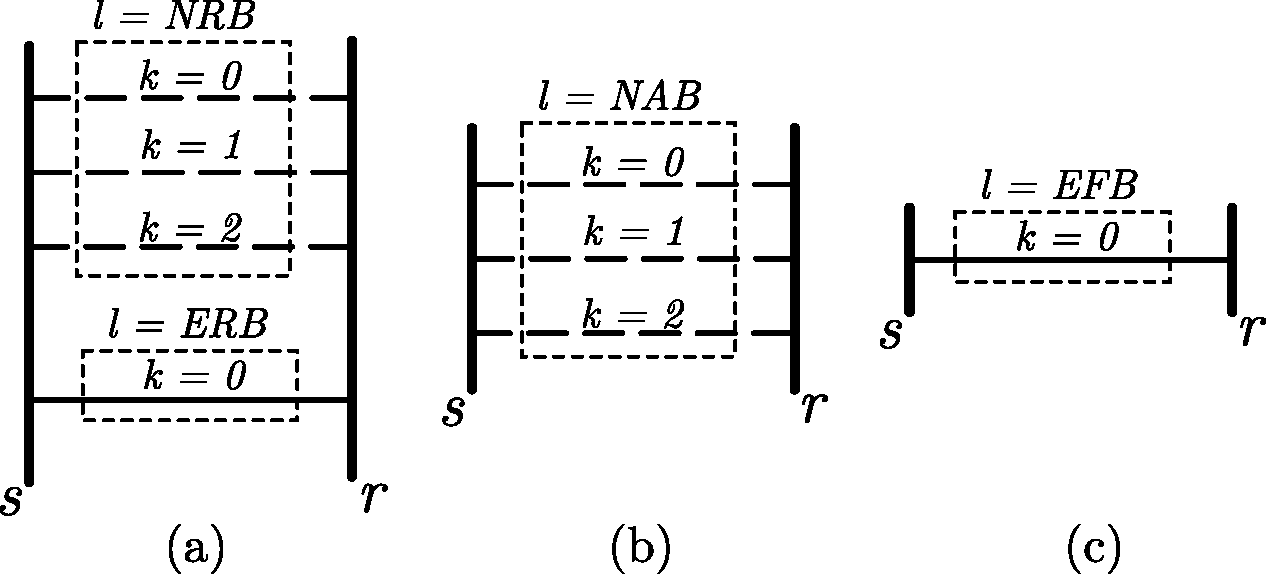
\includegraphics[width=0.8\textwidth]{cap2/ramos.pdf}
%     \\\vspace{1em}Fonte: Proprio Autor
%     \label{fig:ramos}
% \end{figure}

Note que entre dois nós, pode haver mais de um tipo de condutor. Este caso ocorre apenas para os ramos que podem ser substituíveis, visto que há o conjunto de condutores existentes ($ERF$) e novos ($NRF$). Nos outros tipos de ramos há apenas um tipo de condutor, seja novo para ser incluído ($NAF$) ou existente fixo ($EFF$). Os ramos para inclusão não estão fisicamente no sistema de distribuição antes da expansão e podem ser incluídos durante a expansão. Já os ramos existentes fixos estão previamente no sistema de distribuição e não podem sofrer alterações durante a execução do plano de expansão.

Do ponto de vista da modelagem matemática, não há diferença entre ramos e condutores, visto que todos os ramos/condutores são indexados nas mesmas variáveis. Nesta modelagem, todos os ramos/condutores estão conectados no sistema de distribuição e a variável  $y^l_{srkt}$ é responsável por "acionar" \; esses condutores. A solução do modelo retorna quais condutores serão "acionados"  \; (abstração de escolhidos) para a conexão de nós em cada estágio do plano de expansão.

De forma análoga, a abstração de acionamento é modelada também para a construção de subestações, instalação de novos transformadores e geradores distribuídos. Este tipo de modelagem permite a utilização de variáveis binárias em que 0 significa que o equipamento não será instalado e 1 significa que será instalado.

Este modelo também utiliza a linearização do comportamento do sistema de distribuição proposta por \citeonline{Haffner2008} que avalia o sistema de distribuição pela injeção de corrente de cargas, transformadores e geradores distribuídos. Esta linearização é uma versão adaptada do modelo de sistemas de transmissão e pressupõem que: todas as correntes possuem o mesmo fator de potência e a diferença de tensão entre os dois nós é igual a diferença do módulo de tensão entre eles. 
Nas subseções a seguir serão descritos os equacionamentos matemáticos do modelo, explicando a função objetivo, restrições e as alterações que foram implementadas durante o andamento desta pesquisa.

\subsection{Função objetivo}
\label{sec:fobj}

A função objetivo do modelo de \ac{PESD} utilizado é expressada nas equações \eqref{eq:fobj} e \eqref{eq:descriFobj}, nas quais representam o valor presente do custo total do plano de expansão. Essa função objetivo assume que os custos de investimentos são amortizados para cada estágio do planejamento e todos os equipamentos instalados são utilizados até o final de suas vidas úteis e substituídos por outro idêntico. Também considera-se que cada estágio tem duração de um ano ao assumir uma taxa de juros anual. Esse mesmo tipo de formulação é utilizada nos trabalhos de \citeonline{Lotero2011}, \citeonline{MunozDelgado2015}  e \citeonline{7462292}.
\begin{equation}
    \text{min     } c^{TPV}
    \label{eq:fobj}
\end{equation}
\begin{align}
     c^{TPV}  = & \sum_{t\in T} \left[ \frac{(i +i)^{-t}}{i} c^I_t + (i +i)^{-t} (c^M_t + c^E_t+ c^R_t)\right] 
       +\frac{(i +i)^{-n_T}}{i} (c^M_{n_T}  + c^E_{n_T} + c^R_{n_T})
     \label{eq:descriFobj}
\end{align}

Como pode ser visto, o modelo não utiliza energia não suprida em seu equacionamento. Esta escolha de modelagem força o modelo a sempre atender todas as cargas do plano e reduz o espaço de busca por uma solução. 
Cada custo considerado é expresso nas equações de \eqref{eq:invest} a \eqref{eq:perdas}, nas quais, cada item de investimento, manutenção, energia e perdas possui custos fixos associados a sua classe.

Cada custo de investimento possui fatores de conversão para o \ac{VPL}, conforme a indicado a seguir: $RR^l = (i(1+i)^{\eta^l})/((1+i)^{\eta^l} - 1), \forall l \in \{NFB, NAB\}$; $RR^{NT} = (i(1+i)^{\eta^{NT}})/((1+i)^{\eta^{NT}} - 1)$;
$RR^{DG}_p = (i(1+i)^{\eta^{DG}_p})/((1+i)^{\eta^{DG}_p} - 1)$; $RR^{SS} = (i(1+i)^{\eta^{SS}})/((1+i)^{\eta^{SS}} - 1)$. Estes fatores de conversão consideram que ao final da vida útil de cada equipamento, ele será substituído por outro idêntico até o fim do horizonte de planejamento.

Em \eqref{eq:invest} o custo com investimento para cada estágio é formulado. Os investimentos que podem ser realizados são: substituição ou adição de novas linhas, expansão de subestações existentes e adição de novas, instalação de novos transformadores nas subestações e instalação de geradores distribuídos.

% Diferente do modelo de \citeonline{MunozDelgado2015}, são considerados apenas geradores distribuídos despacháveis. Esta consideração é realizada devido a necessidade da empresa distribuidora poder controlar a potência injetada de cada gerador distribuído e assim ter uma segurança sobre a operação do sistema no contexto de \ac{HC}. Outro motivo é devido ao modelo original não lidar com o comportamento estocástico de geradores distribuídos de fontes renováveis e, na opinião do autor, isto acaba sendo uma aproximação que pode ocasionar outros problemas durante a operação do sistema de distribuição planejado. Por outro lado, formulações que consideram o comportamento estocástico de geradores distribuídos de fontes renováveis costumam aumentar consideravelmente a quantidade de variáveis de decisão e restrições, dificultando assim a resolução do problema de \ac{PESD}, como pode ser visto no trabalho de \citeonline{Asensio2018}.

\begin{align}
     c^I_t  = & \sum_{l\in \{NRB, NAB\}} RR^l  \sum_{k\in K^l} \sum_{(s,r)\in \Upsilon^l}C^{I,l}_k \ell_{sr}x^l_{srkt}
     + RR^{SS}  \sum_{s \in \Omega^{SS}} C^{I,SS}_k x^{SS}_{st} \nonumber\\
     &+ RR^{NT}  \sum_{k\in K^{NT}} \sum_{s \in \Omega^{SS}}  C^{I,NT}_k x^{NT}_{st}
     +\sum_{p\in P}  RR^{DG}_p \sum_{k\in K^{DG}_p} \sum_{s \in \Omega^{DG}_p} C^{I,DG}_{pk} pf\overline{G}^{DG}_{pk} x^{DG}_{pskt};\nonumber\\ &\forall t \in T
     \label{eq:invest}
\end{align}

Em \eqref{eq:manu} descreve-se os custos com a manutenção de cada elemento utilizado no sistema de distribuição. Da mesma forma que o equacionamento dos investimentos, cada elemento utilizado possui o custo fixo de manutenção. 

\begin{align}
     c^M_t  = & \sum_{l\in L}  \sum_{k\in K^l} \sum_{(s,r)\in \Upsilon^l} C^{M,l}_k (y^l_{srkt} + y^l_{rskt})
     + \sum_{tr \in TR} \sum_{k\in K^{tr}} \sum_{s \in \Omega^{SS}} C^{M,tr}_k y^{tr}_{skt}\nonumber\\
     &+ \sum_{p\in P} \sum_{k\in K^{DG}_p}\sum_{s \in \Omega^{DG}_p} C^{M,DG}_{pk} y^{DG}_{pskt}; \; \; \forall t \in T
     \label{eq:manu}
\end{align}

Em \eqref{eq:energia} apresenta-se o custo com produção de energia.\footnote{Durante as simulações realizadas para a implementação do modelo base do problema de \ac{PESD}, foi observado que a consideração do custo de produção de energia causa alguns problemas de convergência para a solução ótima do modelo ao se utilizar a estratégia de \textit{gap} relativo (ou tolerância absoluta relativa) no algoritmo de Branch \& Bound.
Ao se utilizar um gap de 0,1\% (a fim de se aproximar da solução ótima do problema) os custos com energia se mantém próximos à solução de 1\% reportada no artigo original, porém, os outros custos, opções de investimento e a topologia do sistema de distribuição são completamente diferentes e o tempo computacional aumenta exponencialmente com a redução do valor de gap. Isto ocorre devido aos custos de produção de energia serem mais de 85\% dos custos totais das soluções encontradas durante as simulações. Por outro lado, não considerar os custos de produção de energia torna indiferente uma das maiores vantagens de geradores distribuídos baseados em eólico e solar: não haver custos de geração, apenas manutenção. Desta forma, foi decidido manter este custo com produção de energia.}, seja da compra de energia provinda da transmissão, seja pela geração distribuída instalada

\begin{align}
    c^E_t  =
    \sum_{b \in B} \Delta_b pf\bigg[
    \sum_{tr \in TR} \sum_{k \in K^{tr}} \sum_{s \in \Omega^{SS}}
    C^{SS}_b g^{tr}_{sktbh} + 
    \sum_{p \in P}\sum_{k \in K^{DG}_p} \sum_{s \in \Omega^{DG}_p} C^{E, \;DG}_{pk}  g^{DG}_{psktbh}\bigg]; \nonumber\; \;\\ \forall t \in T, h=E 
    \label{eq:energia}
\end{align}
 

Em \eqref{eq:perdas} são equacionadas as perdas relacionadas aos transformadores e linhas utilizadas. Como pode-se observar há dois fatores quadráticos no problema e segundo \citeonline{Lotero2011} e \citeonline{MunozDelgado2015} a presença destes dois fatores pode causar dificuldades na busca por soluções do problema. 

\begin{align}
 c^R_t  =
\sum_{b \in B} C^{SS}_b \Delta_b pf \bigg[&\sum_{tr \in TR} \sum_{k \in K^{tr}} \sum_{s \in \Omega^{SS}} Z^{tr}_k (g^{tr}_{sktbh})^2  +\nonumber \\
&\sum_{l \in L} \sum_{k \in K^l} \sum_{(s, r) \in \Upsilon^l} Z^l \ell_{sr} (f^l_{srktbh} + f^l_{rsktbh})^2
\bigg]; \; \; \forall t \in T, h=E 
\label{eq:perdas}
\end{align}

Desta forma, é demonstrada  a seguir a estratégia utilizada para a linearização dos termos quadráticos. 

\subsubsection*{Linearização das perdas}

Os termos quadráticos são linearizados conforme descrito e utilizado por \citeonline{Gonen1981, Lotero2011, MunozDelgado2015}. Esta estratégia utiliza a linearização por partes e mais detalhes podem ser vistos em \citeonline{Gonen1981}. Desta forma a equação \eqref{eq:perdas} é substituída pelas equações de \eqref{eq:perdas_lin} a \eqref{eq:perdas_lin2}. No modelo proposto, o parâmetros da linearização são definidos como: $M^{l}_{k\nu} = (2\nu - 1)Z^l_k \overline{F}^l_k/n_\nu$; $M^{tr}_{k\nu} = (2\nu - 1)Z^{tr}_k\overline{G}^{tr}_k/n_\nu$; $ A^l_{k\nu} = \overline{F}^l_k/n_\nu$; $A^{tr}_{k,\nu} = \overline{G}^{tr}_k/n_\nu$.

\begin{align}
 c^R_t  =
   \sum_{b \in B} C^{SS}_b \Delta_b pf \bigg[&\sum_{tr \in TR} \sum_{k \in K^{tr}} \sum_{s \in \Omega^{SS}}
   \sum_{\nu = 1}^{n_\nu}
   M^{tr}_{k\nu} \delta^{tr}_{sktb\nu} +\nonumber \\
    &\sum_{l \in L} \sum_{k \in K^l} \sum_{(s, r) \in \Upsilon^l}
    \sum_{\nu = 1}^{n_\nu}
    \ell_{sr}M^{l}_{k\nu} (\delta^l_{srktb\nu} + \delta^l_{rsktb\nu})
    \bigg]; \; \; \forall t \in T
    \label{eq:perdas_lin}
\end{align}
\begin{align}
    &g^{tr}_{sktbh} = \sum_{\nu = 1}^{n_\nu}\delta^{tr}_{sktb\nu}; \; \; \forall tr \in TR, \forall s \in \Omega^{SS}, \forall k \in K^{tr}, \forall t \in T, \forall b \in B, h=E\\
    &\delta^{tr}_{sktb\nu} \leq A^{tr}_{k,\nu}; \; \; \forall tr \in TR, \forall s \in \Omega^{SS}, \forall k \in K^{tr}, \forall t \in T, \forall b \in B, \forall \nu \in \{1,...,n_\nu\}\\
    &f^l_{srktbh} = \sum_{\nu = 1}^{n_\nu}\delta^l_{srktb\nu}; \; \;\forall l \in L, \forall s \in \Omega^N, \forall r \in \Omega^l_s, \forall k \in K^l, \forall t \in T, \forall b \in B, h=E\\
    &\delta^l_{srktb\nu} \leq A^l_{k\nu}; \; \;\forall l \in L, \forall s \in \Omega^N, \forall r \in \Omega^l_s, \forall k \in K^l, \forall t \in T, \forall b \in B , \forall \nu \in \{1,...,n_\nu\}
    \label{eq:perdas_lin2}
\end{align}

\subsection{Restrições de comportamento do sistema e limites operacionais}

Neste conjunto de restrições, é definido o comportamento do sistema de distribuição ao uso das linhas, transformadores e geradores distribuídos instalados. Também são definidos os limites operacionais em regime permanente: tensão, ampacidade de condutores, corrente de injeção de transformadores e de geradores distribuídos.

Em \eqref{eq:lim_tensao} define-se os limites de tensão em cada barramento do sistema. Observa-se que, em todo caso, as tensões nos nós do sistema de distribuição devem permanecer dentro dos limites operacionais e que as tensões dos nós são definidos como uma variável de decisão real do problema de \ac{PESD}.
\begin{align}
    \underline{V} \leq v_{stbh} \leq \overline{V}; \; \;& \forall s \in \Omega^N, \forall t \in T, \forall b \in B, \forall h \in H
    \label{eq:lim_tensao}
\end{align}


Já de \eqref{eq:amp} até \eqref{eq:lim_rw} são definidos os limites operacionais das linhas, transformadores e geradores distribuídos. Diferente do modelo original, as restrições de injeção de corrente dos transformadores e geradores distribuídos existem para todos os nós do sistema de distribuição.

\begin{align}
   f^{l}_{srktbh} \leq y^l_{srkt} \overline{F}^l_k; \; \; &\forall l \in L, \forall r \in \Omega^N, \forall s \in \Omega^{l}_r, \forall k \in K^{l}, \forall t \in T, \forall b \in B, \forall h \in H
   \label{eq:amp}
\end{align}
\begin{align}%Restrição alterada:   A variáveis de injeção do trafo possui limites para todas as barras
   g^{tr}_{sktbh} \leq y^{tr}_{skt} \overline{G}^{tr}_k; \; \; &\forall tr \in TR, \forall b \in B, \forall t \in T,  \forall s \in \Omega^{N}, \forall k \in K^{tr}, \forall h \in H
   \label{eq:ijec}
\end{align}
\begin{align}%Restrição alterada:   A variáveis de injeção de DG possui limites para todas as barras
   g^{DG}_{psktbh} \leq y^{DG}_{pskt}\overline{G}^{DG}_{pk}; \; \; &\forall p \in D,  \forall s \in \Omega^{N}, \forall k \in K^{DG}_p, \forall t \in T, \forall b \in B, \forall h \in H
   \label{eq:lim_dg}
\end{align}
\begin{align}
   g^{DG}_{psktbh} =  & \;y^{DG}_{pskt} \alpha^{RW}_h \text{ min} \left( \overline{G}^{DG}_{pk}, G^{RW}_{psktb} \right); \nonumber\\&\forall p \in RW,  \forall s \in \Omega^{N}, \forall k \in K^{DG}_p, \forall t \in T, \forall b \in B, \forall h \in H
   \label{eq:lim_rw}
\end{align}

Observe que a equação \eqref{eq:lim_rw} é uma adição em relação ao modelo original e que não há um limite de injeção de corrente relacionado às cargas do sistema. Este limite de injeção foi retirado devido ao objetivo de identificar a capacidade de acomodação de geradores distribuídos. Já a equação \eqref{eq:lim_rw} foi inserida pois o modelo proposto neste trabalho não considera que geradores renováveis podem ser despachados. Por outro lado, considera que há cenários (representados por $\alpha^{RW}_h$). Estes cenários podem considerar, por exemplo, $\alpha^{RW}_h = 0$, indicando que não há geração renovável no cenários $h$ (caso de intermitências nas fontes de energia).

Por fim, são descritas as equações do comportamento do sistema de distribuição, na qual, \eqref{eq:corrent_balanc} está relacionada à lei de Kirchhoff das correntes e \eqref{eq:tensao} descreve o comportamento da tensão ao longo dos alimentadores. Observa-se que esta formulação só é possível devido às suposições do modelo relacionadas ao fator de potência e diferença de tensão descritas anteriormente.
\begin{align}
    \sum_{l \in L}\sum_{k \in K^{l}} \sum_{r \in \Omega^l_s} (f^{l}_{srktbh} - f^{l}_{rsktbh}) =
    \sum_{tr \in TR} \sum_{k \in K^{tr}} g^{tr}_{sktbh} + \sum_{p\in P} \sum_{k \in K^{DG}_p} g^{DG}_{psktbh} - \mu_bD_{st};  \nonumber\\
    \forall s \in \Omega^N, \forall t \in T, \forall b \in B, \forall h \in H
    \label{eq:corrent_balanc}
\end{align}
\begin{align}
&y^l_{srkt}[Z^l_{k}\ell_{sr}f^l_{srktbh} - (v_{stbh} - v_{rtbh})] = 0; \nonumber\\
&\forall l \in L, \forall r \in \Omega^N, \forall s \in \Omega^{l}_r, \forall k \in K^{l}, \forall t \in T, \forall h \in H
\label{eq:tensao}
\end{align}

Entretanto, \eqref{eq:tensao} não é linear devido à multiplicação entre duas variáveis. Este problema pode ser solucionado utilizando a linearização por disjunção (\textit{Big M}) descrita a seguir.

\subsubsection*{Linearização da equação de diferença de tensão}

Esta linearização ativa e desativa uma restrição dado uma variável de decisão binária. Desta forma, \eqref{eq:tensao} pode ser substituída por \eqref{eq:tensao1} e \eqref{eq:tensao2}. Este tipo de linearização é conhecido por gerar alguns problemas de convergência no uso de métodos de solução de programação linear inteira-mista. Porém, em \citeonline{Confiability_Munoz} é relatado que assumindo $M = \overline{V} -  \underline{V}$ não é observado problemas de convergência.
\begin{align}
&- Z^l_{k}\ell_{sr}f^l_{srktbh} + (v_{stbh} - v_{rtbh}) \leq  M(1 - y^l_{srkt}); \nonumber\\
&\forall l \in L, \forall r \in \Omega^N, \forall s \in \Omega^{l}_r, \forall k \in K^{l}, \forall t \in T, \forall b \in B, \forall h \in H
 \label{eq:tensao1}\\
&Z^l_{k}\ell_{sr}f^l_{srktbh} - (v_{stbh} - v_{rtbh}) \leq  M(1 - y^l_{srkt}); \nonumber\\
&\forall l \in L, \forall r \in \Omega^N, \forall s \in \Omega^{l}_r, \forall k \in K^{l}, \forall t \in T, \forall b \in B, \forall h \in H
\label{eq:tensao2}
\end{align}

\subsubsection*{Restrições de domínio adicionadas ao modelo}

Em \eqref{eq:volt_sub} são descritas as tensões fixas dos nós de subestações que possuem transformadores.
\begin{align}
v_{stbh} = V^{SS} \sum_{tr \in TR}\sum_{k \in K^{tr}} y^{tr}_{skt} ; \; \;& \forall s \in \Omega^{SS}, \forall t \in T, \forall b \in B, \forall h \in H
\label{eq:volt_sub}
\end{align}

De \eqref{eq:dom1} até \eqref{eq:dom3} é descrita a não utilização de geradores distribuídos e transformadores em barramentos não permitidos\footnote{A notação \textbf{S}$_1\setminus$\textbf{S}$_2$ significa: O conjunto \textbf{S}$_1$ com exceção dos elementos no conjunto \textbf{S}$_2$.}.

\begin{align}
    y^{DG}_{pskt} = 0; \;\; \forall p \in P, \forall s \in \Omega^N \setminus \Omega^{DG}_p , \forall k \in K^{DG}_p, \forall t \in T
\label{eq:dom1}\\
    y^{tr}_{skt} = 0; \;\; \forall tr \in TR,  \forall s \in \Omega^N \setminus \Omega^{SS} , \forall k \in K^{tr}, \forall t \in T
\label{eq:dom2}\\
    y^{ET}_{skt} = 0; \;\; \forall s \in \Omega^{SSN} , \forall k \in K^{ET}, \forall t \in T
\label{eq:dom3}
\end{align}


\subsection{Restrições lógicas e de investimento}

Para o planejamento correto dos equipamentos instalados, as restrições lógicas são descritas abaixo.

As restrições de \eqref{eq:inv_feeder} até \eqref{eq:inv_trafo} descrevem que no máximo um tipo de investimento em linhas, subestações, transformadores e geradores distribuídos, respectivamente podem ser usados por vez.
\begin{equation}
    \sum_{t \in T} \sum_{k \in K^l} x^l_{srkt} \leq 1; \; \forall l \in \{NRB, NAB\}, \forall (s,r) \in \Upsilon^l
    \label{eq:inv_feeder}
\end{equation}
\begin{equation}
    \sum_{t \in T} x^{SS}_{st} \leq 1; \; \forall s \in \Omega^{SS}
    \label{eq:inv_sub}
\end{equation}
\begin{equation}
    \sum_{t \in T} \sum_{k \in K^{NT}} x^{NT}_{skt} \leq 1; \; \forall s \in \Omega^{SS}
    \label{eq:inv_trafo}
\end{equation}
\begin{equation}
    \sum_{t \in T} \sum_{k \in K^{DG}_p} x^{DG}_{pskt} \leq 1; \; \forall p \in P, \forall s \in \Omega^{DG}_p
    \label{eq:inv_DG}
\end{equation}

Em \eqref{eq:inv_trafo_sub} descreve-se a relação entre investimento de novos transformadores e novas subestações de forma que ao se criar uma nova subestação, deve-se investir também em um transformador na mesma.
\begin{equation}
    x^{NT}_{st} \leq \sum_{\tau =1}^t x^{SS}_{s\tau}; \; \forall s \in \Omega^{SS}, \forall k \in K^{NT}, \forall t \in T
    \label{eq:inv_trafo_sub}
\end{equation}

As restrições de \eqref{eq:feeder_eff} a \eqref{eq:feeder_sub} descrevem, respectivamente: ramos fixos que não podem ser alterados, ramos que podem ser substituídos ou adicionados devem ser utilizados caso haja investimento, linhas que podem ser substituídas não permanecem após novos investimentos nas mesmas (são substituídas). Diferente do modelo original, este modelo não permite troca de alimentador após uma decisão de investimento. Isto força o modelo de antemão decidir ramos que não passarão por alterações nos outros estágios, diminuindo o espaço soluções e permitindo uma melhor convergência. Estas restrições seguem a mesma modelagem utilizada no trabalho de \citeonline{Asensio2018}.
\begin{align}%Restrição corrigida. #Ref: DOI: 10.1109/TSG.2016.2560339
    y^{EFB}_{srkt} + y^{EFB}_{rskt} =  1; \; \; \forall (s,r) \in \Upsilon^{EFB},  \forall k \in K^{EFB}, \forall t \in T
    \label{eq:feeder_eff}\\
 %Restrição corrigida. #Ref: DOI: 10.1109/TSG.2016.2560339
    y^{l}_{srkt} + y^{l}_{rskt} = \sum_{\tau = 1}^{t} x^l_{srk\tau}; \; \; \forall l \in \{NRB, NAB\}, \forall (s,r) \in \Upsilon^{l},  \forall k \in K^{l}, \forall t \in T
    \label{eq:feeder_new}\\
 %Restrição corrigida. #Ref: DOI: 10.1109/TSG.2016.2560339
    y^{ERB}_{srkt} + y^{ERB}_{rskt} =  1 - \sum_{\tau = 1}^{t}\sum_{k \in K^{NFB}} x^{NRB}_{srk\tau}; \; \; \forall (s,r) \in \Upsilon^{ERB},  \forall k \in K^{ERB}, \forall t \in T
    \label{eq:feeder_sub}
\end{align}

Por fim, as restrições de \eqref{eq:trafo_new1} a \eqref{eq:DG_new1} descrevem a relação entre uma decisão de investimento e a utilização de transformadores e geradores distribuídos, respectivamente.
\begin{equation}
    y^{NT}_{skt} \leq \sum_{\tau = 1}^{t} x^{NT}_{sk\tau}; \; \forall s \in \Omega^{SS}, \forall k \in K^{NT}, \forall t \in T
    \label{eq:trafo_new1}
\end{equation}
\begin{equation}
    y^{DG}_{pskt} \leq \sum_{\tau = 1}^{t} x^{DG}_{psk\tau}; \; \forall p \in P,  \forall s \in \Omega^{DG}_p, \forall k \in K^{DG}_p, \forall t \in T
    \label{eq:DG_new1}
\end{equation}

\subsubsection*{Restrições de Investimento}

Sobre os investimentos, a restrição \eqref{eq:orca_lim} descreve que todos os investimentos realizados em um determinado estágio do \ac{PESD} não podem ultrapassar o limite estabelecido pelo parâmetro de orçamento $IB_t$.
\begin{align}
\sum_{s \in \Omega^{SS}} C^{I,SS}_{k} x^{SS}_{st} + \sum_{k \in K^{NT}} \sum_{s \in \Omega^{SS}} C^{I,NT}_{k} x^{NT}_{skt} +
\sum_{l\in \{NFB,NAB\}} \sum_{k \in K^l} \sum_{(s,r) \in \Upsilon^l} C^{I,l}_{k} \ell_{sr}x^l_{srkt} +\nonumber\\
\sum_{p\in P}\sum_{k\in K^{DG}_p} \sum_{s \in \Omega^{DG}_p} C^{I,DG}_{pk} pf\overline{G}^{DG}_{pk} x^{DG}_{pskt} \leq IB_t; \; \;\forall t \in T
\label{eq:orca_lim}
\end{align}

\subsubsection*{Restrições de domínio adicionadas ao modelo}

Da mesma forma que anteriormente, a restrição \eqref{eq:trafo_domin} foi adicionada no modelo e descreve que no máximo um tipo de transformador deve ser utilizado nos barramentos que já possuem subestações.
\begin{align}
    \sum_{tr \in TR} \sum_{k \in K^{tr}} y^{tr}_{skt} \leq 1 ; \;\; \forall s \in \Omega^{SSE} , \forall t \in T
    \label{eq:trafo_domin}
\end{align}

\subsection{Restrições de radialidade}

De forma que o sistema de distribuição planejado seja radial ao final do plano, as restrições \eqref{eq:radi1} e \eqref{eq:radi2} são utilizadas. Estas restrições são as mesmas utilizadas inicialmente por \citeonline{Haffner2008}, porém, conforme discutido em \citeonline{Lotero2011} elas são necessárias mas não são suficientes para a radialidade na presença de geradores distribuídos.
\begin{align}
    \sum_{l \in L}\sum_{s \in \Omega^l_r}\sum_{k \in K^l} y^l_{srkt} = 1; \forall r \in \Omega^{LN}_t, \forall t \in T
    \label{eq:radi1}
\end{align}
\begin{align}
    \sum_{l \in L}\sum_{s \in \Omega^l_r}\sum_{k \in K^l} y^l_{srkt} \leq 1; \forall r \in \Omega^{N} \setminus \Omega^{LN}_t, \forall t \in T
    \label{eq:radi2}
\end{align}

\subsubsection*{Restrições de radialidade propostas}

No trabalho de \citeonline{MunozDelgado2015}, se utiliza a estratégia de injeções de corrente fictícias nos barramentos em que podem ser instalados geradores distribuídos, evitando possíveis ilhamentos. Entretanto, estas restrições de radialidade adicionais utilizavam pressupostos (como o de substituição de ramos já planejados) que não fazem parte do modelo proposto nesta tese.  Por tanto, é proposta as restrições de \eqref{eq:radi3} até \eqref{eq:radi4} para lidar com a radialidade.

\begin{align}
    \sum_{r \in \Omega^S_s} \widetilde{f}_{srt} - \widetilde{f}_{srt} = \widetilde{g}_{st}^{SS} - \widetilde{d}_{st};\;\; \forall s \in \Omega^N, \forall t \in T
    \label{eq:radi3}
\end{align}
\begin{align}
     \widetilde{f}_{srt} \leq n_{DG} \sum_{l\in L} \sum_{k \in K^l} y^l_{srkt};\;\; \forall s \in \Omega^N, \forall r \in \Omega^S_s, \forall t \in T
\end{align}
\begin{align}
     \widetilde{g}_{st}^{SS} \leq n_{DG}\sum_{tr\in TR} \sum_{k \in K^{tr}} y^{tr}_{skt};\;\; \forall s \in \Omega^{SS}, \forall t \in T
\end{align}
\begin{align}
     \widetilde{g}_{st}^{SS} = 0;\;\; \forall s \in \Omega^{N} \setminus \Omega^{SS}, \forall t \in T
\end{align}
\begin{align}
     \widetilde{d}_{st} = \sum_{p \in D} \sum_{k \in K^p} y^{DG}_{pskt};\;\; \forall s \in \Omega^N, \forall t \in T
     \label{eq:radi4}
\end{align}

Observe que estas restrições criam uma demanda fictícia onde há geradores distribuídos despacháveis, forçando que haja fluxo de corrente fictício entre os ramos, gerados por algum nó que há um transformador. Desta forma, é evitado que haja um nó ilhado. Nós que possuem geradores distribuídos renováveis, não podem criar nós ilhados, pois um dos cenários que deve ser avaliado ($\alpha^{RW}$) em \eqref{eq:corrent_balanc} deve ser o cenário de não geração devido as intermitências das fontes de energia.

\subsection{Restrições de domínio}


Para facilitar a reprodutibilidade do modelo utilizado, seguem abaixo as restrições de domínio.

\subsubsection*{Variáveis reais}

As restrições de \eqref{eq:dom_ctpv} a \eqref{eq:dom_ci} descrevem o domínio das variáveis de custos.
\begin{align}
    &c^{TPV} \geq 0 \label{eq:dom_ctpv}\\
    &c^E_t \geq 0; \; \;\forall t \in T \\
    &c^M_t \geq 0; \; \;\forall t \in T \\
    &c^R_t \geq 0; \; \;\forall t \in T \\
    &c^I_t \geq 0; \; \;\forall t \in T \label{eq:dom_ci}
\end{align}

Já as restrições \eqref{eq:dom_corr} e \eqref{eq:dom_corr_fict} descrevem o domínio das variáveis de corrente entre nós reais e fictícias.
\begin{align}
f^l_{srktbh} \geq 0; \; \;\forall l \in L, \forall s \in \Omega^N, \forall r \in \Omega^l_s, \forall k \in K^l, \forall t \in T, \forall b \in B , \forall h \in H \label{eq:dom_corr}\\
\widetilde{f}_{srt} \geq 0; \; \;\forall s \in \Omega^N, \forall r \in \Omega^S_s, \forall t \in T, \forall b \in B
\label{eq:dom_corr_fict}
\end{align}

As restrições de \eqref{eq:dom_gdg} a \eqref{eq:dom_gss} descrevem respectivamente o domínio das variáveis de injeção de corrente dos geradores distribuídos, transformadores e de subestação fictícia.
\begin{align}
&g^{DG}_{psktbh} \geq 0; \; \; \forall p \in P, \forall s \in \Omega^N, \forall k \in K^{DG}, \forall t \in T, \forall b \in B , \forall h \in H \label{eq:dom_gdg}\\
&g^{tr}_{sktbh} \geq 0; \; \; \forall tr \in TR, \forall s \in \Omega^N, \forall k \in K^{tr}, \forall t \in T, \forall b \in B , \forall h \in H \\
&\widetilde{g}^{SS}_{st} \geq 0; \; \; \forall s \in \Omega^N, \forall t \in T, \label{eq:dom_gss}\\
&\widetilde{d}_{st} \geq 0; \; \; \forall s \in \Omega^N, \forall t \in T 
\end{align}

Por fim, a restrição \eqref{eq:dom_volt} descreve o domínio das variáveis de tensão nodal.
\begin{equation}
    v_{stbh} \geq 0; \; \; \forall s \in \Omega^N, \forall t \in T, \forall b \in B , \forall h \in H \label{eq:dom_volt}
\end{equation}

\subsubsection*{Variáveis inteiras}

Em relação às variáveis de utilização dos equipamentos, as restrições de \eqref{eq:dom_linha} a \eqref{eq:dom_dg} descrevem respectivamente sobre o domínio dos equipamentos: linhas, transformadores e geradores distribuídos.
\begin{align}
    &y^l_{srkt} \in \{0, 1\}; \; \; \forall l \in L, \forall s \in \Omega^N, \forall r \in \Omega^l_s, \forall k \in K^l, \forall t \in T \label{eq:dom_linha}\\
    &y^{tr}_{skt} \in \{0, 1\}; \; \; \forall tr \in TR, \forall s \in \Omega^{N}, \forall k \in K^{TR}, \forall t \in T\\
    &y^{DG}_{pskt} \in \{0, 1\}; \; \; \forall p \in P, \forall s \in \Omega^{N}, \forall k \in K^{DG}_p, \forall t \in T \label{eq:dom_dg}
\end{align}

Já em relação às variáveis de investimento dos equipamentos, as restrições de \eqref{eq:dom_inv_linha} a \eqref{eq:dom_inv_dg} descrevem respectivamente sobre o domínio dos equipamentos: linhas, transformadores, expansão de subestações e geradores distribuídos.
\begin{align}
    &x^l_{srkt} \in \{0, 1\}; \; \; \forall l \in \{NRB, NAB\}, \forall s \in \Omega^N, \forall r \in \Omega^l_s, \forall k \in K^l, \forall t \in T \label{eq:dom_inv_linha}\\
    &x^{NT}_{skt} \in \{0, 1\}; \; \; \forall s \in \Omega^{SS}, \forall k \in K^{NT}, \forall t \in T\\
    &x^{SS}_{st} \in \{0, 1\}; \; \; \forall s \in \Omega^{SS}, \forall t \in T\\
    &x^{DG}_{pskt} \in \{0, 1\}; \; \; \forall p \in P, \forall s \in \Omega^{DG}_p, \forall k \in K^{DG}_p, \forall t \in T \label{eq:dom_inv_dg}
\end{align}

\subsubsection*{Variáveis reais de linearização}

Por fim, as restrições \eqref{eq:dom_lin_perdas1} e \eqref{eq:dom_lin_perdas2} descrevem o domínio das variáveis de linearização das perdas.
\begin{align}
    &\delta^l_{srktb\nu} \geq 0 \; \; \forall l \in L, \forall s \in \Omega^N, \forall r \in \Omega^l_s, \forall k \in K^l, \forall t \in T, \forall b \in B, \forall \nu \in \{1, ..., n_\nu \} \label{eq:dom_lin_perdas1}\\
    &\delta^{tr}_{sktb\nu} \geq 0 \; \; \forall tr \in TR, \forall s \in \Omega^{SS}, \forall k \in K^{TR}, \forall t \in T, \forall b \in B, \forall \nu \in \{1, ..., n_\nu \} \label{eq:dom_lin_perdas2}
\end{align}

\newpage
\subsection{Vantagens e desvantagens do modelo base}

Observa-se que o modelo base utilizado neste trabalho não representa exatamente o comportamento de sistemas de distribuição devido às linearizações realizadas. Por outro lado, este modelo é linear inteiro-misto e este tipo de modelagem matemática já possui métodos bem consolidados e softwares para a solução bem otimizados. A fim de validar o modelo utilizado, uma versão simplificada foi utilizada na publicação do artigo \cite{9281945} que investiga o modelo de planejamento base sob a perspectiva de uma grande número de alternativas de condutores (primeira página disponível no Apêndice \ref{sec:paperPESD}), este modelo base também auxiliou nas contribuições feitas em \cite{9916750}.

Tanto \citeonline{Haffner2008} quanto \citeonline{MunozDelgado2015} argumentam que a representação aproximada das equações que regem o comportamento de sistemas de distribuição é suficiente do ponto de vista de \ac{PESD}, no qual, muitas vezes é elevado o nível de incerteza relacionado tanto a alguns parâmetros de entrada (níveis de carregamento, preços, etc.) quanto a alguns parâmetros de saída do problema (tensões, correntes, perdas, etc.). Além desta incerteza, muitas vezes a empresa distribuidora necessita apenas de um valor estimado dos custos do \ac{PESD} para uma tomada de decisão mais estratégica para o modelo de negócio.

De todo modo, vale ressaltar que o modelo apresentado neste trabalho possui um comportamento otimista em relação ao real comportamento que o sistema de distribuição irá apresentar após a execução do plano e que nem todos os problemas observados em sistemas de distribuição são considerados. Desta forma, recomenda-se utilizar este modelo como uma estimativa inicial dos custos de investimento relacionados ao problema de \ac{PESD}. Para uma avaliação mais concreta sobre o sistema de distribuição final, outros estudos são necessários para a tomada de decisão final, como por exemplo a avaliação do desequilíbrio de tensão, alocação de dispositivos de proteção, dispositivos de regulação de tensão, medidores e estrutura de monitoramento, entre outros.

Portanto, a escolha deste modelo para a utilização tanto no problema de \ac{PESD} quanto para a avaliação do \ac{HC} é justificada tanto pela facilidade de implementação do modelo em softwares de alto desempenho, quanto pelo o contexto e objetivos no qual este trabalho se encontra. No próximo capítulo, aprofundamentos nos conceitos de \ac{HC} e sua integração neste modelo serão apresentados.
\chapter{Capacidade de Acomodação de Recursos Energéticos Distribuídos}

Neste capítulo, são apresentados os principais conceitos e aspectos de \ac{HC}. Inicialmente é apresentado brevemente o contexto em que este conceito se aplica em sistemas de distribuição, na qual a presença de geradores distribuídos já é uma realidade e há uma perspectiva de aumento nos anos seguintes. Em seguida, este contexto é confrontado com a dificuldade de se mensurar a capacidade que sistemas de distribuição têm de acomodar novos geradores distribuídos e como este problema se relaciona com o \ac{PESD}. Desta forma, são apresentadas as principais abordagens encontradas na literatura para identificar, mensurar e melhorar o valor de \ac{HC}, bem como as considerações realizadas para tal. Por fim, é apresentada a proposta de integração de um indicador de \ac{HC} no modelo de \ac{PESD} abordado no capítulo anterior.

Esta proposta é baseada no espelhamento das restrições de comportamento do sistema de distribuição do modelo base, no qual cria-se novas variáveis para as tensões nodais, fluxo de corrente nos ramos e injeção de corrente dos transformadores e geradores distribuídos. A partir deste espalhamento cada nó recebe a nova variável que representa a injeção de corrente de futuros recursos energéticos distribuídos. Por fim, é adicionado na função objetivo base um novo parâmetro que busca maximizar o valor da soma destas novas injeções. Desta forma, e no mesmo modelo, é possível avaliar tanto o custo com o \ac{PESD}, quanto o \ac{HC} de cada nó e do sistema por inteiro. Por outro lado, algumas limitações podem ser observadas no modelo de modo que uma análise numérica destas limitações se torna necessária. Esta análise é realizada no próximo capítulo deste trabalho, porém, alguns levantamentos e possíveis problemas já são abordados neste. 

Ao final deste capítulo, espera-se que o contexto atual em que os sistemas de distribuição se encontram e a problemática relacionada à grande presença de geradores distribuídos esteja clara, bem como a proposta de integração do problema de \ac{PESD} e da métrica adotada para o \ac{HC}.


\section{Conceitos sobre a capacidade de acomodação}


O problema da integração de recursos energéticos distribuídos em sistemas de distribuição vem sendo discutido desde o surgimento destes geradores. Atualmente, observa-se que há uma tendência de tornar o sistema de distribuição mais controlável, principalmente devido aos problemas causados pelas intermitências das fontes renováveis destes geradores. Esta tendência se traduz no conceito de \textit{smart grid} que pode ser definido como um sistema altamente observável por meio de medições e controlável remotamente (incluindo de forma autônoma) através dos mais diversos dispositivos instalados. Por outro lado,  segundo \citeonline{Tuballa2016710}, observa-se que muitas tecnologias relacionadas ao conceito de \textit{smart grid} ainda estão em fase de pesquisa e desenvolvimento e, principalmente em países em desenvolvimento, este conceito pode levar alguns anos (até décadas) para ser amplamente adotado. 

Neste contexto de transição, surge o conceito de capacidade de acomodação de recursos energéticos distribuídos (\ac{HC}), no qual é um indicador de alta abstração do sistema de distribuição que demonstra a quantidade e potência máxima de recursos energéticos distribuídos que podem ser instalados. Ao utilizar este indicador, os engenheiros de planejamento da empresa distribuidora e outros investidores podem avaliar a disponibilidade de novos investimentos sem a necessidade de grandes alterações no sistema de distribuição, tornando estas tomadas de decisões mais claras e objetivas.

Além de avaliar o indicador, também é possível realizar alterações no sistema de distribuição com o objetivo de melhorar este indicador. Estas alterações podem fazer parte do plano de \ac{PESD}, alterando a topologia do sistema, alocação de novos dispositivos ou alterações da proteção do sistema de distribuição. Por outro lado, a melhoria do indicador também pode fazer parte da operação, utilizando chaves para alterações topológicas, chaveamento de banco de capacitores, controlando geradores distribuídos despacháveis ou sistemas de armazenamento de energia. Desta forma, pode-se afirmar que qualquer alteração no sistema de distribuição pode melhorar ou piorar o indicador de \ac{HC}, seja de uma forma temporária, durante a operação, ou permanente através do \ac{PESD}.

De modo geral, a figura \ref{fig:hc} demonstra a curva de desempenho de um sistema de distribuição com e sem melhoria do \ac{HC}. Pode-se observar que até certo valor de penetração de recursos energéticos distribuídos o sistema de distribuição possui uma operação aceitável, porém com o aumento da penetração a operação do sistema passa a não ser aceitável, violando algum limite operacional ou de equipamentos. 


\begin{figure}[ht]
 	\centering
    \caption{Curva de desempenho de um sistema de distribuição em relação à penetração de geradores distribuídos e sua capacidade de acomodação antes e depois de uma melhoria.}
    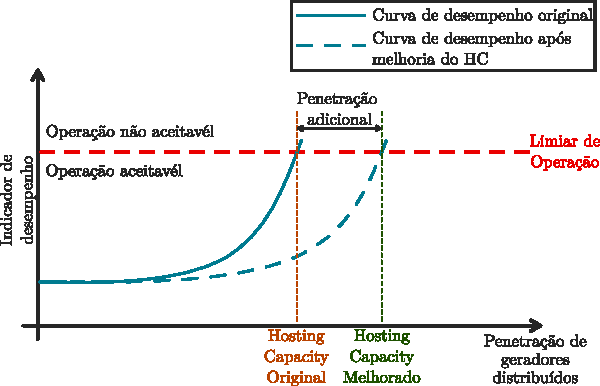
\includegraphics[width=0.8\textwidth]{cap3/HC.pdf}\\
    Fonte: Adaptado de \citeonline{HCStateArt}
    \label{fig:hc}
\end{figure}

A forma de obter o valor de \ac{HC} varia de acordo com a metodologia adotada. Para \citeonline{smith2012stochastic}, em seu relatório para o Electric Power Research Institute, o \ac{HC} pode ser definido através de violação de tensão, carregamento de linhas, dispositivos de proteção, qualidade de energia e controle. Já para \citeonline{palmintier2016path}, em seu relatório para o Departamento de Energia dos Estados Unidos, o \ac{HC} é a capacidade de instalação de novos recursos energéticos distribuídos de um sistema de distribuição sem alteração topológica, instalação de novos dispositivos ou recondutoramento. 


De qualquer forma, podemos definir duas classes de \ac{HC}, o global e o local. O \ac{HC} local é capacidade máxima que uma região ou barramento do sistema possui de instalação de novos recursos energéticos distribuídos. O \ac{HC} global é capacidade máxima que um sistema de distribuição, como um todo, possui de instalação de novos recursos energéticos distribuídos. 
Estes novos recursos energéticos distribuídos, geralmente buscam obter alguma vantagem financeira, seja por serviços ancilares para o sistema de distribuição, seja por redução dos custos com energia elétrica de outras empresas, há também a utilização para arbitragem, porém, geralmente sistemas de armazenamento de energia são mais recomendados nesta operação.
No Brasil, os serviços ancilares ainda não são regulamentados e, portanto, os novos recursos energéticos distribuídos, geralmente buscam redução de custos com energia elétrica ou venda de energia em mercados livres.
Desta forma, o termo \ac{HC} vem sendo amplamente utilizado como forma de indicar quanto um sistema de distribuição pode hospedar recursos energéticos distribuídos não ancilares.

Este crescimento na penetração de recursos energéticos distribuídos não ancilares, vem se tornando uma das principais preocupações das empresas distribuidoras, visto que a presença desses geradores causam diversas perturbações na qualidade de energia, operação e segurança do sistema de distribuição. Segundo o trabalho de \citeonline{HCStateArt}, estima-se um aumento de 58\% nos custos da operação dos sistemas, sendo que 55\% deles atingirão seus limites operacionais nos próximos 10 anos, caso esse crescimento de recursos energéticos distribuídos se mantenha.

Vale salientar que  a empresa distribuidora raramente pode prever a futura existência de recursos energéticos distribuídos de outras empresas em seu sistema de distribuição durante a fase de planejamento. Porém, é de grande importância que a empresa distribuidora possua uma estimativa do valor de \ac{HC} do seu sistema durante esta fase, pois, este indicador ajuda a demonstrar a viabilidade de novos investimentos de outras empresas em seu sistema de distribuição. 

Dentro deste contexto, as empresas distribuidoras vêm realizando diversos esforços para mensurar e para melhorar o valor de HC de seus sistemas de distribuição. E estes esforços se traduzem também nos trabalhos acadêmicos que têm demonstrado interesse neste tema, como será apresentado a seguir.

\section{Capacidade de acomodação na literatura acadêmica}

Segundo \citeonline{en10091325}, o conceito de HC foi inicialmente cunhado por André Even em Março de 2004 durante discussões no projeto EU-DEEP project. Em artigos acadêmicos, este conceito é primeiramente encontrado em \citeonline{Bollen2005} ao descrever os problemas de qualidade de energia relacionados à inserção de recursos energéticos distribuídos em sistemas de distribuição. Segundo \citeonline{Bollen2005} o cálculo de HC deve ser realizado para diversos fenômenos da operação e planejamento e que este valor não é fixo e depende também da estrutura do sistema de distribuição. Neste mesmo artigo o autor apresenta que há um possível \textit{trade-off} entre os custos de investimento no sistema de distribuição e a melhoria do valor de HC. Apesar desta afirmação, o autor se ateve aos problemas de qualidade da energia, descrevendo algumas formas de calcular o HC para os problemas de qualidade da tensão e de harmônicas.

Entretanto, o termo HC e sua análise só obteve adesão considerável por parte da literatura acadêmica a partir de 2014. Um indicador desta adesão pode ser vista na figura \ref{fig:scopus} que demonstra o número de artigos em revistas científicas indexados no sistema Scopus da Elsevier (um dos maiores indexadores de trabalhos acadêmicos do mundo) durante o período de 2005 a 2020 utilizando a query:

\vspace{-1pt}
\noindent\textit{TITLE-ABS-KEY ( "Hosting Capacity" )  AND  PUBYEAR  >  2004  AND  PUBYEAR  <  2021  AND  ( LIMIT-TO ( SUBJAREA ,  "ENGI" )  OR  LIMIT-TO ( SUBJAREA ,  "ENER" ) )  AND  ( LIMIT-TO ( DOCTYPE ,  "ar" ) )}


\begin{figure}[ht]
 	\centering
    \caption{Quantidade de artigos indexados no sistema Scopus da Elsevier durante o período de 2006 a 2020 (entre 2005 e 2009 não houve artigos).}
    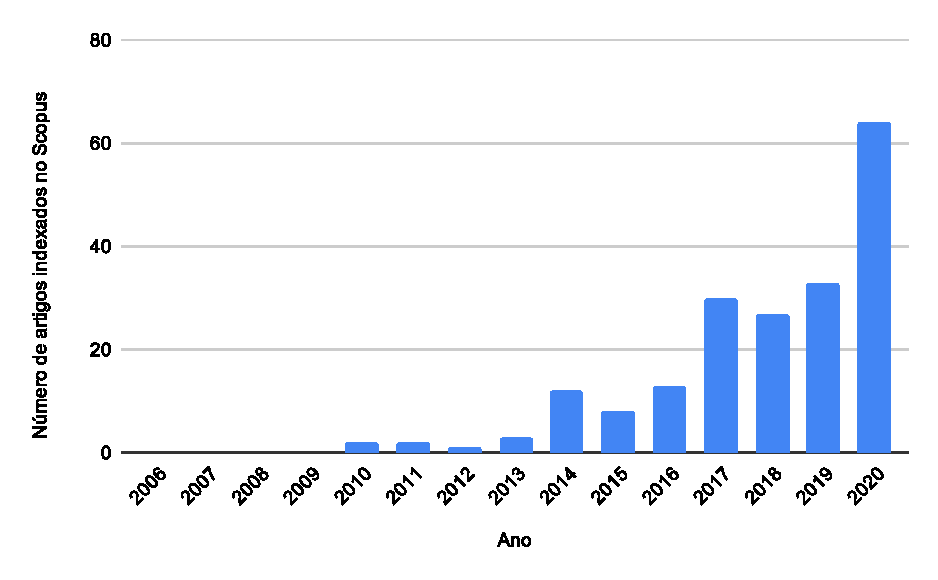
\includegraphics[width=0.8\textwidth]{cap3/chart.pdf}\\
    Fonte: Adaptado de \citeonline{scopus}
    \label{fig:scopus}
\end{figure}

Uma tese sobre esta adesão tardia ocorreu devido ao consenso acadêmico anterior de que a empresa distribuidora teria um grande poder de decisão relacionado a localização, potência instalada e operação de recursos energéticos distribuídos no sistema de distribuição. Este consenso acadêmico da época levou diversos trabalhos acadêmicos até os dias atuais a considerarem que a empresa distribuidora pode decidir o melhor planejamento destes geradores. Curiosamente, uma síntese do estado da arte destes tipos de trabalhos foi publicada por \citeonline{6307952} um ano antes de uma maior adesão acadêmica do termo HC. Atualmente, pode-se afirmar que a empresa distribuidora atua muito mais como um limitador da quantidade e potência de recursos energéticos distribuídos no sistema de distribuição do que um operador destes geradores, com exceção dos geradores com objetivos ancilares.


Outra hipótese sobre esta adesão ter ocorrido a partir de 2014 foi o crescimento de recursos energéticos distribuídos de fontes renováveis em sistemas de distribuição da Europa desde 2004, causados pelos incentivos fiscais e financeiros realizados na \citeonline{eurotstat}.

Nesta revisão da literatura, apenas os trabalhos que lidam diretamente com \ac{HC} foram incluídos, visto que, com a popularização do termo, muitos trabalhos apresentam a melhoria do \ac{HC} como um efeito secundário em relação ao real objetivo do trabalho. Dentre os trabalhos que abordam o conceito de \ac{HC}, podemos dividir estes trabalhos nos seguintes tópicos abaixo que serão explicados a seguir:

\begin{itemize}
    \item formas de mensurar e avaliar a capacidade de acomodação;
    \item medidas de melhoria da capacidade de acomodação por integração do controle da operação dos recursos energéticos distribuídos;
    \item medidas de melhoria da capacidade de acomodação por controle de outros dispositivos no sistema de distribuição.
\end{itemize}
\vfill 

\subsection{Formas de mensurar e avaliar a capacidade de acomodação}

Neste tópico, os trabalhos discutem aspectos sobre quais fatores devem ser considerados ao se avaliar o valor de \ac{HC} de um sistema de distribuição de forma prática, seja durante a operação ou para o planejamento.

Dentre estes trabalhos, está incluso o trabalho de \citeonline{Bollen2005} que discute os como mensurar os impactos de geradores distribuídos na qualidade da energia. Já o trabalho de \citeonline{PAPAIOANNOU2014141} descreve uma metodologia analítica para identificar a melhor localização de um gerador distribuído em um sistema de distribuição de baixa tensão. No trabalho de \citeonline{SANTOS2015199} são descritos os impactos nos componentes harmônicos com o aumento da presença de geradores distribuídos baseados em inversores e propõem uma metodologia para definir o \ac{HC} do sistema de distribuição deste ponto de vista. 

Partindo de um outro ponto de vista, o trabalho de \citeonline{en8031760} descreve o impacto de carregadores de veículos elétricos em sistemas de distribuição de baixa tensão e aplica o conceito de \ac{HC} para este novo tipo de dispositivo no sistema de distribuição. No mesmo tópico de avaliar novos recursos distribuídos, o trabalho de \citeonline{7155600} avalia o comportamento de recursos distribuídos de baixo impacto ambiental em sistemas de distribuição de baixa tensão e indica que as avaliações realizadas podem ser utilizadas na avaliação do  \ac{HC}.

O trabalho de \citeonline{7219464} utilizou a mesma estratégia de analisar o comportamento, só que aplicado a geradores distribuídos, para determinar diversas correlações entre a potência, localização e \ac{HC} em sistemas de distribuição e propor uma metodologia simples para avaliar o \ac{HC} de sistemas de distribuição.

O trabalho de \citeonline{en10091325} realiza uma discussão sobre o conceito de \ac{HC} para o planejamento de sistemas de distribuição, nele uma análise para os piores casos de sobretensão e subtensão é realizada e uma discussão sobre os outros problemas são relacionados aos problemas de tensão discutidos. Por fim, é salientado que dados sobre outros recursos distribuídos são necessários para uma análise mais profunda sobre este conceito.

No trabalho de \citeonline{7723860} avalia-se o caso de geradores distribuídos fotovoltaicos e descreve um modelo para estimar o HC utilizando simulação de Monte Carlo para considerar o comportamento estocástico destes geradores. Utilizando uma estratégia parecida, o trabalho de \citeonline{7913608} propõe a determinação do HC através de risco associado devido às incertezas de geradores distribuídos renováveis. Já no trabalho de \citeonline{8270364} foi desenvolvida a mesma estratégia para verificar os riscos relacionados ao HC de geradores distribuídos fotovoltaicos em 50 mil sistemas de distribuição de baixa tensão e foi identificado um comportamento log-normal no risco de violação dos indicadores de HC.  O trabalho de  \citeonline{7763786} baseia-se nos dados obtidos via simulação de sistemas de distribuição ativos para determinar de forma robusta o valor de HC através de otimização linear.


Por outro lado, o trabalho de \citeonline{8325320} realiza uma linearização do problema de HC para desenvolver um método de avaliação do valor através da proposição de um \textit{framework} probabilístico que considera as incertezas da geração distribuída. Em \citeonline{ALTURKI2018350} é proposto outro modelo linearizado para determinar o valor de HC de um sistema de distribuição, segundo os autores, os resultados são obtidos mais rapidamente porém com um pequeno erro. Já no trabalho de \citeonline{Sousa2020}, uma margem prática de estimar o valor de HC é proposta para sistemas de distribuição de baixa tensão com geradores distribuídos fotovoltaicos com inversores inteligentes.

Analisando veículos elétricos, o trabalho de \citeonline{7817888} descreve o conceito de região "carregável", na qual descreve a quantidade de demanda de carregamento de veículos elétricos que um sistema de distribuição pode acomodar em um determinado momento. Esta análise é realizada através de otimização considerando que a empresa distribuidora pode atrasar um carregamento. 

Já o conceito de HC dinâmico foi melhor desenvolvido no trabalho de \citeonline{en12132576} que descreve que um sistema de distribuição possui três níveis de HC: pior, o médio e o melhor, estes valores variam no tempo e no local de estudo. Para esta avaliação, foi verificado o impacto das distorções harmônicas e variação de tensão causados por geradores distribuídos fotovoltaicos.

\subsection{Medidas de melhoria da capacidade de acomodação por integração do controle da operação dos geradores distribuídos} \label{hc_review_control_dg}

Neste tópico, são descritos os métodos que pressupõem um controle sobre o recurso energético distribuído por parte da empresa distribuidora, seja pela utilização de inversores distribuídos inteligentes ou por contratos com os donos dos geradores.

Dentro deste conceito, podemos elencar o trabalho de \citeonline{CALDERARO201464} que descreve uma estratégia de gerenciamento de geradores distribuídos de fontes renováveis através do controle da potência ativa e reativa evitando que estes geradores sejam desconectados por limites de tensão, em seus resultados é observado que um gerenciamento desses recursos poderiam aumentar a capacidade de acomodação do sistema de distribuição. Na mesma direção, o trabalho de \citeonline{6744682} descreve uma estratégia de gerenciamento ativo para melhorar a capacidade de acomodação de geradores eólicos em sistemas de distribuição através da redução da energia gerada, mudança de taps de reguladores e geração de energia reativa, o autor obteve resultados que demonstravam que um gerenciamento destes geradores e de outros dispositivos no sistema de distribuição podem aumentar a capacidade de acomodação de geradores distribuídos. 

Outra estratégia utilizando gerenciamento ativo do sistema de distribuição é proposta por \citeonline{Quijano2017}, no qual busca minimizar as perdas do sistema de distribuição enquanto maximiza a capacidade de injeção de potência dos geradores distribuídos instalados. Unindo estes controles com a possibilidade de recondutoramento, o trabalho de \citeonline{8678766} já propõe uma avaliação estocástica via simulação de Monte Carlo para melhoria do HC de geradores distribuídos fotovoltaicos. 


O trabalho de \citeonline{7534843} explora os aspectos de planejamento multiestágio da alocação de geradores distribuídos no sistema de distribuição com o objetivo de maximizar o valor de HC. Esse planejamento passa pela coordenação probabilística da operação entre os geradores distribuídos, sistemas de armazenamento de energia e dispositivos de geração de potência reativa, neste trabalho também é observado um modelo de planejamento linear diferente dos modelos propostos no problema do \ac{PESD}. Já no trabalho de \citeonline{RABIEE2017417} é proposta a maximização do HC através da otimização da operação de grandes usinas de geração eólica. O trabalho de \citeonline{en12193610} desenvolve um planejamento integrado entre o sistema de transmissão e o valor esperado de HC de sistemas de distribuição ligados à transmissão.

O trabalho de \citeonline{COLLINS2015464} descreve a eficácia do controle de potência ativa e reativa de geradores distribuídos baseados em inversores para a melhoria do HC do ponto de vista de sobre tensão.  Já \citeonline{HU2016264} descreve uma coordenação entre \acp{OLCT} e inversores de geradores distribuídos fotovoltaicos para o gerenciamento de sistemas de distribuição desbalanceados e descreve em seus resultados que esta coordenação eleva consideravelmente o valor de HC. No trabalho de \citeonline{8046055} é utilizado técnicas de gestão ativa do sistema de distribuição para avaliar um valor robusto de HC através de otimização linear inteira-mista. 

Uma análise da sensibilidade de sistemas de distribuição a geradores distribuídos fotovoltaicos foi realizado no trabalho de \citeonline{7784836}, no qual, também propõem que avaliação do HC passa por um modelo de otimização que define as variáveis de controle de sistemas de distribuição ativas (chaveamento de banco de capacitores, reguladores de tensão, alteração na topologia e controle dos inversores dos geradores).

Um estudo mais aprofundado do impacto da possibilidade de controle dos geradores distribuídos baseados em inversores foi realizado por \citeonline{8895828}. Os resultados apontam para uma melhoria considerável no valor de HC quando há a possibilidade de controle de potência ativa e reativa destes geradores.
\vfill

\subsection{Medidas de melhoria do HC por controle de outros dispositivos no sistema de distribuição}

Nesta seção estão descritos os métodos e trabalhos que propõe a melhoria do HC através apenas do controle de outros dispositivos no sistema de distribuição, seja em um contexto de \textit{smart grids} ou não.


O trabalho de \citeonline{6818426} é um dos primeiros trabalhos que parte do problema clássico de reconfiguração do sistema de distribuição para a melhoria do HC. Este trabalho baseia-se na premissa da existência de chaveamento remoto e é baseado no modelo de fluxo de potência ótimo. O conceito de HC é definido pelos limites de tensão em estado permanente e limites térmicos das linhas de distribuição, os autores salientam que o trabalho está inserido no contexto de planejamento da operação pois o problema exigiu um poder computacional e tempo considerável. Baseado no mesmo problema, \citeonline{8279492} propõe a utilização de um algoritmo de decisão \textit{fuzzy} e métodos meta-heurísticos de otimização para determinar uma boa reconfiguração. Já no trabalho de \citeonline{en13205446}, \textit{soft open points} são adicionados no problema de reconfiguração através de um problema de otimização multiobjetivo que busca minimizar perdas enquanto maximiza o valor de HC.

Já o trabalho de \citeonline{7426863} descreve a utilização de \ac{OLCT} e de compensadores de potência reativa estáticos para avaliar o HC considerando que estes chaveamentos são realizados pela empresa distribuidora durante o planejamento da operação. Seguindo a discussão de utilização de novos dispositivos, o trabalho de \citeonline{LONG2016427} propõe a utilização de \textit{soft open points} para aliviar o carregamento das linhas e problemas com sobretensão e, assim, melhorar o HC. Já o trabalho de \citeonline{7317829} descreve uma estratégia utilizando o \ac{OLCT}, banco de capacitores e um sistema de monitoramento aplicado a sistemas de distribuição de baixa tensão para melhoria do HC. 


Através de mecanismos de resposta da demanda no contexto de \textit{smart grids}, o trabalho de \citeonline{SOROUDI2017316} busca obter um equilíbrio entre as perdas do sistema de distribuição e melhoria do valor de HC, este problema é modelado na forma de otimização bi-objetiva não linear. Já avaliando apenas compensadores de potência reativa estáticos, o trabalho de \citeonline{XU2019952} propõe um planejamento ótimo da alocação e operação desses dispositivos e identifica que há uma melhoria significativa do HC para geradores distribuídos fotovoltaicos. Por outro lado, o trabalho de \citeonline{8481391} já propõe um controle adaptativo destes dispositivos baseando-se no conceito de HC dinâmico. Já um gerenciamento das cargas em sistemas de distribuição de baixa tensão baseado em programação linear é proposto por \citeonline{Bakhtiari2020}, no qual poucos dados compartilhados entre os consumidores e a empresa de distribuição são necessários.

Através de aspectos práticos (como por exemplo, rebalanceamento de cargas nas fases do sistema), o trabalho de \citeonline{Wong2017} propõe diversas medidas que podem ser adotadas antes de necessariamente aplicar conceitos de \textit{smart grids} em sistemas de distribuição de baixa tensão para melhorar o HC. Já no trabalho de \citeonline{8360415} através da análise dos resultados obtidos por uma otimização meta-heurística, é proposto um índice prático para o recondutoramento de linhas de distribuição para melhoria do valor de HC.

Analisando os problemas relacionados às componentes harmônicas, o trabalho de \citeonline{SAKAR201774} descreve como filtros passivos podem ser utilizados para a melhoria do valor de HC na presença de muitos geradores distribuídos fotovoltaicos.

\subsection{Análise da literatura acadêmica}

Durante esta revisão da literatura acadêmica sobre o assunto, observou-se que muitos trabalhos que tratam sobre a definição de HC avaliam o problema sobre os indicadores de tensão em regime permanente e limites operacionais das linhas de distribuição, sobre uma perspectiva estocástica que considera o comportamento tanto da carga quanto das fontes de energia dos recursos energéticos distribuídos. Baseado nos estudos desenvolvidos durante esta análise, uma forma de estimar os impactos da tensão em regime permanente dos recursos energéticos distribuídos foi desenvolvido e publicado em \cite{MONTEIRO2023109190}, a primeira página deste artigo pode ser vista no Apêndice \ref{sec:paperDER}. 

Pode-se observar que muitos trabalhos estão relacionados com um conceito de HC dinâmico que pode ser melhorado através da gestão ou planejamento da operação dos sistemas de distribuição. É observado também uma constante preocupação com os sistemas de distribuição de baixa tensão, visto que muitos não possuem quaisquer tipo de controle ou poucos dados e, desta forma, predominam métodos aproximados de avaliação do HC.

Outro fator relevante observado é a presença de inversores inteligentes que permitem que a empresa distribuidora controle pelo menos a injeção de potência reativa dos geradores distribuídos baseados nestes inversores. Soma-se a isso o contexto de \textit{smart grid}, no qual a empresa também pode realizar diversos tipos de alterações no sistema de distribuição de forma remota e muitas vezes durante a própria operação.

Os trabalhos que lidam com o planejamento de sistemas de distribuição geralmente abordam apenas a operação, com alguns indicando a possibilidade de recondutoramento das linhas dos sistemas. Durante a análise bibliográfica realizada nesta pesquisa até o momento, não foram encontrados outros trabalhos que relacionam o \ac{PESD} com o valor de HC. Porém, em muitos trabalhos é possível observar que os autores indicam uma relação entre os custos com recondutoramento e instalação de novos equipamentos (típico do problema do \ac{PESD})  com a melhoria do valor de HC do sistema de distribuição.


Por fim, observa-se também que há diferentes modelos para avaliar e melhorar o valor de HC e que alguns deles optam por utilizar modelos linearizados do comportamento do sistema de distribuição. O fato de haver pouca literatura que relaciona o problema de PESD com HC e os modelos lineares observados na literatura foram cruciais para a decisão de basear-se no modelo apresentado anteriormente para obter o valor de HC dos sistemas de distribuição resultados do PESD, conforme descrito na próxima seção.

\section{Modelo de otimização para capacidade de acomodação}

Conforme discutido na seção anterior, ainda não há um consenso sobre quais indicadores devem ser utilizados para a definição do valor de \ac{HC} de um sistema de distribuição. Isso se torna mais evidente quando observamos que não foram encontrados trabalhos que relacionam o problema de \ac{PESD} com \ac{HC}. Porém, é observado na literatura que muitos modelos partem do princípio que, no mínimo, os indicadores de HC devem incluir os limites operacionais de tensão e os limites de ampacidade do sistema de distribuição.

De qualquer modo, neste trabalho definimos que o valor de \ac{HC} é a maior quantidade de potência produzida ou demandada por recursos energéticos distribuídos não operados pela empresa distribuidora que pode ser injetada ao longo dos estágios, independentemente do nível de carregamento do sistema de distribuição, referentes aos indicadores de limites de tensão, balanço de potência e os limites de operacionais dos outros ativos instalados.

No modelo de \ac{PESD} base utilizado neste trabalho, estes indicadores já estão inclusos no modelo. Por outro lado, não é possível avaliar o valor de HC apenas com os conjuntos de restrições já existentes, pois não há qualquer forma de calcular o máximo valor de potência que pode ser injetada. 

Ao analisar os modelos de otimização encontrados na literatura, muitos "simulam"\; a alocação de recursos energéticos distribuídos no sistema de distribuição e buscam maximizar a potência instalada destes recursos. Observamos que esta estratégia, sem a adição de novas restrições, impacta diretamente nos custos com investimentos e, portanto, na função objetivo do problema, descaracterizando o objetivo de minimizar os custos de investimento no sistema de distribuição.

Logo, é desejável obter um modelo que consiga mensurar o valor de HC do sistema de distribuição planejado sem descaracterizar o objetivo maior do problema de \ac{PESD} (redução de custos).  Expandindo este objetivo para um \ac{PESD} multiestágio com níveis de carregamento, surgem outras questões:
\begin{itemize}
\item Como "simular"\; o impacto de recursos energéticos distribuídos que ainda não estão no sistema? 
\item Deve-se avaliar o HC apenas para o último estágio? 
\item Se não, cada estágio terá um valor de HC diferente? 
\item Deve-se considerar um HC dinâmico, visto que o modelo base também utiliza níveis de carregamento do sistema?
\end{itemize}

Estas questões são os alvos de discussões sobre o modelo proposto ainda durante a redação deste trabalho. De qualquer modo, optou-se por unificar todas estas questões em apenas um único modelo, porém, recomenda-se que outras formas de abordá-las devem ser fonte de investigações em futuros trabalhos.

A "simulação"\; do impacto de novos recursos energéticos distribuídos é realizado por um espelhamento do comportamento do sistema de distribuição planejado. Este espelhamento é feito utilizando a mesma estrutura das equações de comportamento do sistema de distribuição do modelo base com as mesmas variáveis binárias de uso das linhas e transformadores, porém, utilizando novas variáveis para representar as tensões, corrente nos ramos e injeção de corrente na presença dos novos recursos energéticos distribuídos. As incertezas referentes aos geradores distribuídos renováveis são demonstradas pelos parâmetros $\alpha^{HC}_u$ e $\alpha^{RW}_h$, tanto no modelo de \ac{PESD}, quanto no modelo de \ac{HC}.  Uma ilustração desta estratégia é apresentada na figura \ref{fig:model_hc}.

\begin{figure}[ht]
 	\centering
    \caption{Estratégia utilizada para "simular"\; novos recursos energéticos distribuídos no modelo de PESD.}
    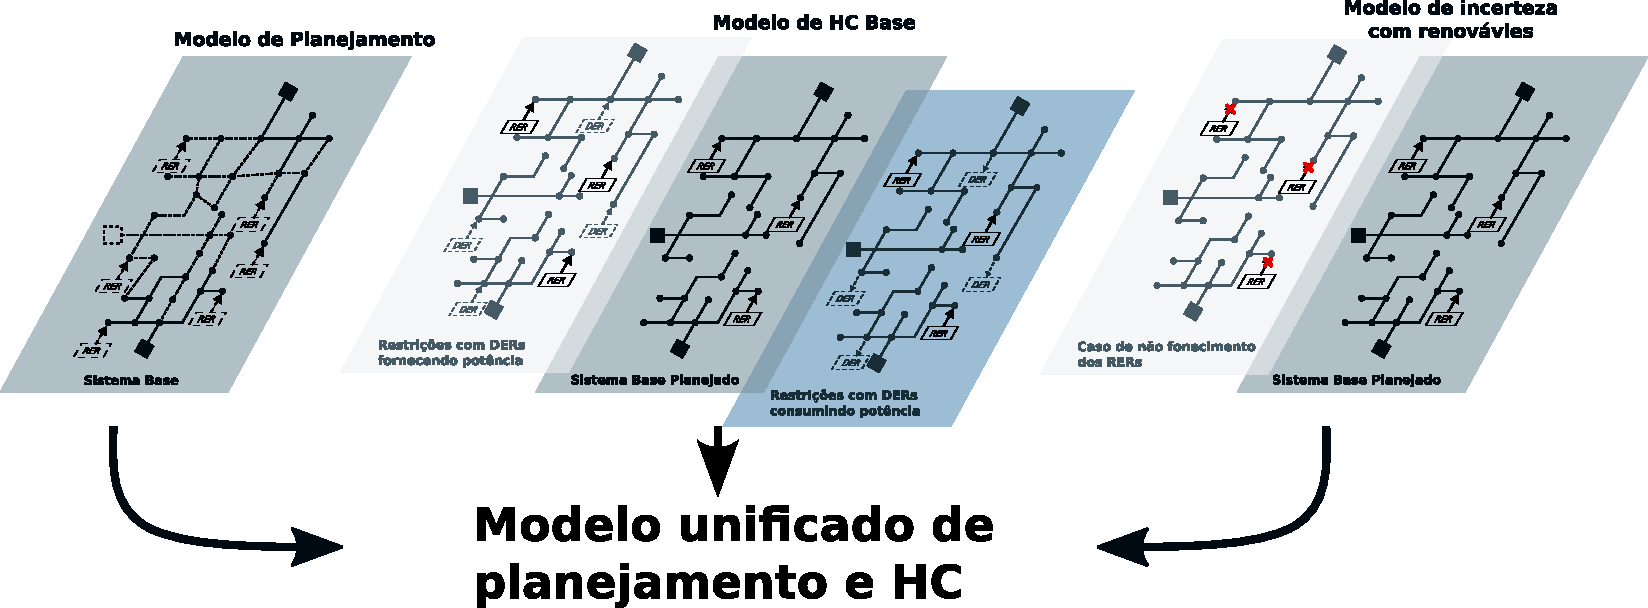
\includegraphics[width=1\textwidth]{cap3/modelo-new.pdf}\\
    Fonte: Próprio autor
    \label{fig:model_hc}
\end{figure}

Optou-se por avaliar o valor do \ac{HC} através do menor valor de injeções de corrente dos recursos energéticos distribuídos em cada estágio. Observa-se que esta proposição assume que cada estágio terá seu valor de \ac{HC}, porém, através da adição de novas restrições, impõe-se que a injeção de corrente deve no mínimo se manter igual durante a evolução dos estágios. 

Não é considerado um \ac{HC} dinâmico, devido ao autor deste trabalho compreender que esta avaliação é melhor feita durante o planejamento da operação, fugindo do escopo do \ac{PESD}. Por fim, considera-se que há um recurso energético distribuído em todos os barramentos do sistema de distribuição que possuem carga, porém, estes recursos só existem nas novas restrições adicionadas.

Também não é considerado o comportamento estocástico de recursos energéticos renováveis assumindo que, durante o \ac{PESD}, a empresa distribuidora não tem conhecimento do tipo de recurso que será instalado. Esta proposição segue a mesma linha de considerar que a empresa distribuidora deve ser responsável por manter o sistema de distribuição operando com qualidade, não importando quais recursos e cargas estão instalados em seu sistema de distribuição. Por outro lado, esta consideração torna a estimativa do valor de  \ac{HC} bastante conservadora, abrindo diversas oportunidades de estudos de melhoria do \ac{HC} via planejamento da operação.

Por outro lado, são considerados cenários de \ac{HC}, nos quais, podem-se simular cenários onde a análise é feita apenas para geradores distribuídos, apenas para carregamento de veículos elétricos, ou para ambos (na forma de armazenadores de energia). Estes cenários são configurados pelo parâmetro $\alpha^{HC}_u$, no qual valores positivos são considerados como geração e negativos como carga.

Desta forma, a seguir são detalhadas as alterações e adições realizadas no modelo base do problema de \ac{PESD} para incluir a estimativa do valor de \ac{HC}.

\subsection{Função objetivo para capacidade de acomodação}

Conforme discutido na revisão bibliográfica, o valor de \ac{HC}  é definido como a máxima injeção possível de recursos energéticos distribuídos no sistema de distribuição. Porém, podemos considerar também um \ac{HC} local, como a máxima injeção possível de recursos energéticos em um nó do sistema de distribuição. De toda forma, foi escolhido neste modelo que todos os nós do sistema injetam a mesma quantidade de corrente ($J^{HC}_t$) no estágio $t$ e que o valor de \ac{HC} no estágio $t$ é a maximização deste valor. O valor de $J^{HC}_t$ também pode ser interpretado como a máxima corrente segura que pode ser injetada em qualquer um dos nós do sistema de distribuição. O indicador escolhido para o \ac{HC} para todos os estágios é a soma da injeção dos nós, conforme descrito em \eqref{eq:fobj_hc}. 
\begin{equation}
    \text{max.    } \sum_{t \in T} J^{HC}_t
    \label{eq:fobj_hc}
\end{equation}

Observe que este indicador é conservador  e deve ser interpretado como uma estimação da capacidade de acomodação dos nós do sistema de distribuição. Desta forma, após a decisão de quais investimentos serão realizados, novos estudos mais detalhados devem ser conduzidos a fim de obter um valor mais aproximado da realidade.


\subsection{Espelhamento do sistema de distribuição}

O espelhado do sistema de distribuição para "simular" os impactos do sistema de distribuição é realizado através da inclusão de novas restrições do comportamento do sistema. De \eqref{eq:lim_tensao_hc} até \eqref{eq:lim_dg_hc} são formulados, respectivamente, os limites operacionais das tensões, ampacidade de linhas, injeção de transformadores e de geradores distribuídos instalados na presença dos novos geradores distribuídos.
 \begin{align}
    \underline{V} \leq v_{stbhu}^{HC} \leq \overline{V}; \nonumber\\  \forall s \in \Omega^N, \forall t \in T, \forall b \in B, \forall h \in h, \forall u \in U
    \label{eq:lim_tensao_hc}\\
   f^{l, HC}_{srktbhu} \leq y^l_{srkt} \overline{F}^l_k;  \nonumber\\ \forall l \in L, \forall r \in \Omega^N, \forall s \in \Omega^{l}_r, \forall k \in K^{l}, \forall t \in T, \forall b \in B, \forall h \in h, \forall u \in U
   \label{eq:amp_hc}\\
   g^{tr, HC}_{sktbhu} \leq y^{tr}_{skt} \overline{G}^{tr}_k;  \nonumber\\ \forall tr \in TR, \forall b \in B, \forall t \in T,  \forall s \in \Omega^{N}, \forall k \in K^{tr}, \forall h \in h, \forall u \in U 
   \label{eq:ijec_hc}\\
   g^{DG,HC}_{psktbhu} \leq y^{DG}_{pskt}\overline{G}^{DG}_{pk};  \nonumber\\ \forall p \in D, \forall s \in \Omega^{DG}_p, \forall k \in K^{DG}_p, \forall t \in T, \forall b \in B, \forall h \in h, \forall u \in U\\
   g^{DG,HC}_{psktbhu} = g^{DG}_{psktbh}; \nonumber\\ \forall p \in RW, \forall s \in \Omega^{DG}_p, \forall k \in K^{DG}_p, \forall t \in T, \forall b \in B, \forall h \in h, \forall u \in U
   \label{eq:lim_dg_hc}
\end{align}

De \eqref{eq:corrent_balanc_hc} a \eqref{eq:tensao2_hc} é descrito o comportamento do sistema de distribuição na presença dos novos geradores distribuídos. Observe que em \eqref{eq:corrent_balanc_hc} a penetração dos novos recursos energéticos é adicionada como uma nova fonte de geração no barramento, impactando o fluxo de corrente nos ramos e, por sequência, nas tensões do sistema de distribuição formulado em \eqref{eq:tensao1_hc} e \eqref{eq:tensao2_hc}.
\begin{align}
    \sum_{l \in L}\sum_{k \in K^{l}} \sum_{r \in \Omega^l_s} (f^{l, HC}_{srktbhu} - f^{l, HC}_{rsktbhu}) = \alpha^{HC}_u g_{st}^{HC} + 
    \sum_{tr \in TR} \sum_{k \in K^{tr}} g^{tr, HC}_{sktbhu} \nonumber \\ + \sum_{p \in P}\sum_{k\in K^{DG}_p} g^{DG, HC}_{psktbhu} - \mu_bD_{st}; \nonumber\\
    \forall s \in \Omega^N, \forall t \in T, \forall b \in B, \forall h \in H, \forall u \in U
    \label{eq:corrent_balanc_hc}
\end{align}
\begin{align}
&- Z^l_{k}\ell_{sr}f^{l, HC}_{srktbhu} + (v_{stbhu}^{HC} - v_{rtbhu}^{HC}) \leq  M(1 - y^l_{srkt}); \nonumber\\
&\forall l \in L, \forall r \in \Omega^N, \forall s \in \Omega^{l}_r, \forall k \in K^{l}, \forall t \in T, \forall b \in B, \forall h \in H, \forall u \in U
 \label{eq:tensao1_hc}\\
&Z^l_{k}\ell_{sr}f^{l, HC}_{srktbhu} - (v_{stbhu}^{HC} - v_{rtbhu}^{HC}) \leq  M(1 - y^l_{srkt}); \nonumber\\
&\forall l \in L, \forall r \in \Omega^N, \forall s \in \Omega^{l}_r, \forall k \in K^{l}, \forall t \in T, \forall b \in B, \forall h \in H, \forall u \in U
\label{eq:tensao2_hc}
\end{align}

Por fim, a restrição \eqref{eq:volt_sub_hc} descreve o comportamento das tensões nos barramentos de subestação. Em \eqref{eq:hc_load} define que a corrente injetada deve ser a mesma em todos os nós. Em \eqref{eq:hc_no_sub} não permite a injeção de novos recursos distribuídos em barramentos sem cargas. Já em \eqref{eq:mantem_gera_tpcco_hc} garante que a injeção de corrente dos novos recursos seja no mínimo a mesma durante a evolução do \ac{PESD}.
\begin{align}
&v_{stbhu}^{HC} = V^{SS} \sum_{tr \in TR}\sum_{k \in K^{tr}} y^{tr}_{skt} ; \; \; \forall s \in \Omega^{SS}, \forall t \in T, \forall b \in B, \forall h \in H, \forall u \in U
\label{eq:volt_sub_hc}\\
&g^{HC}_{st} = J^{HC}_t;\; \; \forall t \in T, \forall s \in   \Omega^{LN}_t\label{eq:hc_load}\\
&g^{HC}_{st} = 0;\; \; \forall t \in T, \forall s \in   \Omega^{N}\setminus \Omega^{LN}_t\label{eq:hc_no_sub}\\
&J^{HC}_{t} \leq J^{HC}_{{t+1}}; \; \; \forall t \in \{1, 2, ..., n_{T} -1 \}
\label{eq:mantem_gera_tpcco_hc}
\end{align}

\vspace{-0.25cm}
\subsection{Restrições de domínio}

Para assegurar uma melhor reprodutibilidade do modelo proposto, segue de \eqref{eq:dom_corr_hc} a \eqref{eq:dom_j_hc} as restrições de domínio das variáveis adicionadas no modelo.
\begin{align}
&f^{l, HC}_{srktbhu} \geq 0; \; \;\forall l \in L, \forall s \in \Omega^N, \forall r \in \Omega^l_s, \forall k \in K^l, \forall t \in T, \forall b \in B , \forall h \in H, \forall u \in U \label{eq:dom_corr_hc}\\
&g^{DG, HC}_{sktbhu} \geq 0; \; \; \forall s \in \Omega^N, \forall k \in K^{DG}, \forall t \in T, \forall b \in B, \forall h \in H, \forall u \in U \label{eq:dom_gd_hc}\\
&g^{tr, HC}_{sktbhu} \geq 0; \; \; \forall tr \in TR, \forall s \in \Omega^N, \forall k \in K^{tr}, \forall t \in T, \forall b \in B, \forall h \in H, \forall u \in U\\
&g^{HC}_{st} \geq 0 ; \; \; \forall s \in \Omega^N, \forall t \in T \label{eq:dom_g_hc}\\
&J^{HC}_{t} \geq 0 ; \; \; \forall t \in T \label{eq:dom_j_hc}
\end{align}

\subsection{Limitações do modelo proposto}

Como o modelo base, o modelo proposto é linear inteiro-misto multiobjetivo, portanto, as mesmas limitações aplicadas ao modelo base aplicam-se a este. Do ponto de vista da estimativa do \ac{HC}, este modelo apresenta uma estimativa conservadora, tanto por assumir o não conhecimento dos geradores distribuídos que podem ser instalados, quanto por buscar maximizar o valor de \ac{HC} via injeção de corrente, dado que a potência depende tanto do valor da corrente, quanto do valor da tensão em cada barramento.

Outra limitação do modelo é considerar a mesma corrente simulada em todos os nós para estimar o \ac{HC}. Este fator, 
torna o modelo ainda mais conservador e não considera outros fatores como \ac{HC} locais diferentes para cada nó, nem leva em consideração outros indicadores de \ac{HC}. Entretanto, este modelo consegue integrar o \ac{PESD} com uma estimativa do \ac{HC}, o que, até o momento, não foram encontradas propostas semelhantes na literatura acadêmica. 

A seguir são demonstrados resultados numéricos dos modelos apresentados.

\chapter{Resultados numéricos}

Neste capítulo, apresenta-se o método numérico de solução do modelo apresentado neste trabalho, os recursos computacionais utilizados, os sistemas que foram testados e as soluções numéricas obtidas. 


Conforme apresentado nos capítulos anteriores, o modelo proposto nesta tese possui duas funções objetivo. A primeira busca minimizar o valor presente líquido dos custos de investimento, manutenção, perdas técnicas e com geração de energia ($c^{TPV}$). A segunda função objetivo busca maximizar a injeção de corrente considerada "segura"\; em quaisquer dos nós do sistema de distribuição ($J^{HC}_t$).

Entretanto, um dos objetivos desta tese é analisar os aspectos que relacionam o valor de \ac{HC} com os custos do \ac{PESD}. Portanto é necessário observar como as alterações no custo do \ac{PESD} impactam o valor de \ac{HC}. Para tal análise, foi escolhido identificar alguns dos \textit{pontos ótimos da Fronteira de Pareto}\footnote{Neste capítulo utiliza-se os seguintes conceitos como sinônimos: ponto ótimo da Fronteira de Pareto, solução ótima da Fronteira de Pareto, solução Pareto-ótima, ponto Pareto-ótimo} do modelo apresentado.

Para os leitores que não estão familiarizados com o conceito de Fronteira de Pareto em otimização ou com técnicas de solução de modelos multi-objetivos, recomenda-se a leitura do artigo de \citeonline{oliveira2010multiobjective}. Porém, de forma geral e resumida, os pontos ótimos da fronteira de Pareto de um modelo bi-objetivo linear inteiro misto, são soluções que satisfazem ambas as funções objetivo e que não há nenhuma outra solução que as \textit{domine}, ou seja, não há outra solução que melhore ainda mais uma das funções objetivos, sem necessariamente degradar a outra. 


\section{Método numérico de resolução}

Sabe-se que comumente é computacionalmente inviável (mesmo que teoricamente possível), obter todas as soluções Pareto-ótimas de modelos complexos. Portanto, métodos numéricos são aplicados para se obter as soluções numéricas Pareto-ótima destes modelos. Dentre várias opções possíveis, foi escolhido o método Hierárquico (também conhecido como Lexicográfico) em conjunto com o método $\epsilon$-restrito (também conhecido como \textit{trade-off}) para a busca de soluções Pareto-ótima do modelo apresentado. Detalhes teóricos, numéricos e específicos de cada método fogem do escopo desta tese, recomenda-se novamente o artigo de \citeonline{oliveira2010multiobjective} para uma introdução ao tema.

No modelo hierárquico, definiu-se que \ac{HC} possui uma hierarquia maior que o os custos do \ac{PESD}, ou seja, na resolução do modelo hierárquico, resolve-se primeiro a função objetivo de \ac{HC} e então fixa-se o valor de \ac{HC} e resolve-se o modelo para a função objetivo de custos do \ac{PESD}.

A figura \ref{fig:method} descreve a implementação destes métodos e como foi feita a integração entre o método Hierárquico com o $\epsilon$-restrito. Os parâmetros de entrada do método utilizado dependem de um valor inicial de $c^{TPV}$ (representada na figura \ref{fig:method} como $c^{TPV - HC}$) e de um valor de $\epsilon$. Estes valores são utilizados para decrementar o limite máximo de $c^{TPV}$ do modelo hierárquico, configurando assim, como um método $\epsilon$-restrito. Nesta abordagem, sugere-se um valor inicial de $c^{TPV - HC}$ grande o suficiente para que na primeira iteração o valor da função objetivo de \ac{HC} seja a maior possível. Nesta tese, utilizou-se $\epsilon = 450$ e $c^{TPV - HC} = 10^{10}$ como entrada para todas as análises.

\begin{figure}[ht]
 	\centering
    \caption{Abordagem para a resolução do modelo bi-objetivo.}
        \begin{tikzpicture}[node distance=2cm]
        \node (start) [startstop] {Início};
        \node (in1) [io, below of=start, xshift=-2.5cm] {Valor inicial de \\ $c^{TPV - HC}$};
        \node (in2) [io, right of=in1, xshift=2.5cm] {Valor de $\epsilon$};
        \node (pro1) [process, right of=start, xshift=5cm] {Resolva o modelo apenas \\ para $c^{TPV}$};
        \node (pro2) [process, below of=pro1] {$c^{TPV - MIN} \leftarrow c^{TPV}$};
        \node (dec1) [decision, below of=in2, yshift=-0.3cm] {$ c^{TPV - HC} - c^{TPV - MIN} > \epsilon$};
        \node (stop) [startstop, right of=dec1, xshift=4.5cm] {Fim};
        \node (pro3) [process, below of=dec1, yshift=-0.5cm] {Adicione nova restrição\\$c^{TPV} \leq c^{TPV - HC} - \epsilon$};
        \node (pro4) [process, below of=pro3] {Resolva o modelo bi-objetivo\\hierárquico};
        \node (out1) [io, right of=pro4, xshift=3.5cm] {Salve\\a solução};
        \node (pro5) [process, left of=pro4, xshift=-3.5cm] {$c^{TPV - HC} \leftarrow c^{TPV}$};
        \node (pro6) [process, above of=pro5] {Remova a restrição\\adicionada};
        \draw [arrow] (start) --  (in1);
        \draw [arrow] (start) -- (in2);
        \draw [arrow] (start) -- (pro1);
        \draw [arrow] (pro1) -- (pro2);
        \draw [arrow] (in1) -- (dec1);
        \draw [arrow] (in2) -- (dec1);
        \draw [arrow] (pro2) -- (dec1);
        \draw [arrow] (dec1) -- node[anchor=south] {Não} (stop);
        \draw [arrow] (dec1) -- node[anchor=east] {Sim} (pro3);
        \draw [arrow] (pro3) -- (pro4);
        \draw [arrow] (pro4) -- (out1);
        \draw [arrow] (pro4) -- (pro5);
        \draw [arrow] (pro5) -- (pro6);
        \draw [arrow] (pro6) |- (dec1);
        \end{tikzpicture}\\
    Fonte: Próprio autor
    \label{fig:method}
\end{figure}

Como todo método $\epsilon$-restrito, a abordagem utilizada possui as mesmas características. Isto significa que valores muito grandes de $\epsilon$ encontrará menos soluções Pareto-ótimas e, portanto, o algoritmo finalizará mais rápido. Já valores muito pequenos de $\epsilon$ encontrará mais soluções Pareto-ótimas, porém, o algoritmo levará mais tempo para finalizar. Teoricamente, com $\epsilon$ tendendo a zero, é possível obter todas as soluções Pareto-ótimas, apesar de ser inviável computacionalmente para modelos complexos.

\section{Recursos computacionais, código fonte e dados}

A implementação e resolução do modelo bi-objetivo foi realizada em um computador Intel i5-8400 com seis núcleos de até 4 GHz, 16 GB de memória RAM DDR4. O computador utilizado executa o sistema operacional Fedora Linux 38 com kernel Linux 6.4. Não foi utilizado processamento com placa de vídeo nesta implementação.

Os modelos e a abordagem de resolução foram implementados em linguagem Julia, uma linguagem de programação livre e de código aberto projetada para atender as demandas atuais de métodos numéricos e programação científica, apresentada no trabalho de \citeonline{Julia-2017}. Foi utilizado também o pacote JuMP para modelagem de problemas de otimização matemática,  apresentado no trabalho de \citeonline{DunningHuchetteLubin2017}. Para a solução do modelo foi utilizado o \textit{solver} Gurobi \cite{gurobi} sob a abstração do pacote Gurobi.jl \cite{gurobijl} em conjunto com o pacote JuMP. As versões de cada \textit{software} são encontradas na tabela \ref{tab:list_soft}.

\begin{table}[ht]
\centering
\caption{Lista de \textit{softwares} utilizados e suas respectivas versões}
\label{tab:list_soft}
\begin{tabular}{@{}lc@{}}
\toprule
\textit{Software} & Versão   \\ \midrule
Julia                              & 1.9.3    \\
JuMP                               & 1.14.0   \\
Gurobi.jl                          & 1.0.3    \\
Gurobi                             & 10.0.2 \\ \bottomrule
\end{tabular}
\\Fonte: Próprio autor
\end{table}

A linguagem, pacotes e \textit{solver} foram escolhidos devido a familiaridade que o autor deste trabalho possui com estes \textit{softwares}, porém, este modelo pode ser implementado em qualquer \textit{solver} de preferência. 

Para a resolução do modelo hierárquico, foi utilizado a abordagem built-in do \textit{solver} Gurobi, configurando a função objetivo de \ac{HC} para prioridade 10 e a função de custos do \ac{PESD} para prioridade 1.

Com o objetivo de fomentar a reprodutibilidade e inspeção dos resultados, todo o código fonte utilizado para a implementação, tanto do modelo base \cite{modelobase}, quanto para o modelo com \ac{HC} \cite{modelocomHC}, estão disponíveis em repositórios Git sob licença Apache v2.0 (uma licença de código aberto e permissiva tanto para cópia, modificação e distribuição). 

Durante a escrita desta tese, o autor trabalha para que os modelos possam ser utilizados como pacotes Julia para serem facilmente importados em trabalhos futuros.


\subsection{Dados de sistemas de distribuição utilizados}

Para demonstrar o modelo e a abordagem proposta, foram utilizados três sistemas baseados em sistemas de distribuição amplamente conhecidos na literatura. Foi necessário realizar alterações nos dados dos sistemas da literatura pois o modelo e a abordagem proposta escalam exponencialmente com o tamanho do modelo e com a quantidade de estágios. Esta desvantagem foi observada após vários meses de implementação, testes e melhoria do código para que fosse possível obter os resultados apresentados nesta tese. Vale ressaltar que as alterações realizadas foram principalmente na quantidade de estágios e nos limites de investimentos. Todos os parâmetros dos modelos podem ser encontrados no repositório Git em \cite{modelocomHC}\footnote{Foi decido não adicionar os dados das redes utilizadas no corpo de texto desta tese, pois, o autor acredita que qualquer forma de reprodução e inspeção das informações contidas neste texto é melhor realizada com o acesso direto aos dados eletrônicos utilizados. Observa-se que a abordagem de prover acesso aos dados diretamente de forma eletrônica é a mesma utilizada em muitos trabalhos publicados atualmente na área de planejamento, veja \citeonline{Confiability_Munoz} e \citeonline{MunozDelgado2015}.}, para serem inspecionados em caso de dúvidas.

O primeiro é o sistema de distribuição de 24 nós que opera a 20 kV, com três estágios de 1 ano cada e uma demanda total máxima de 46,85 MVA no último estágio. Este sistema é baseado no sistema de 24 nós encontrado no trabalho de  \citeonline{MunozDelgado2015}.

O segundo é o sistema de distribuição de 54 nós que opera a 13.5 kV, com um estágio de 3 anos e uma demanda total máxima de 72 MVA. Este sistema é baseado no sistema de 54 nós encontrado no trabalho de  \citeonline{Confiability_Munoz}.

O terceiro é o sistema de distribuição de 138 nós que opera a 13.8 kV, com um estágio de 10 anos e uma demanda total máxima de 38,13 MVA. Este sistema é baseado no sistema de 138 nós encontrado no trabalho de \citeonline{MunozDelgado2015}.





\section{Resultados para o sistema de 24 nós}

Para o sistema de 24 nós, foram realizados três cenários de análise, o primeiro considerando apenas o \ac{HC} para geração distribuída, o segundo considerando o \ac{HC} apenas para veículos elétricos ou novas cargas e o terceiro considerando ambos. Estes cenários podem ser avaliados com a alteração dos parâmetros $\alpha^{HC}$, conforme descrito na seção anterior.

Ao executar a resolução do modelo bi-objetivo para apenas geração distribuída, obteve-se apenas duas soluções, uma com valor de 784 kVA de \ac{HC} e 250,33 milhões de dólares de $c^{TPV}$ e outra com 452 kVA de \ac{HC} e 250,298 milhões de dólares de $c^{TPV}$. Por outro lado, tanto para apenas veículos elétricos ou novas cargas quanto para ambos (veículos elétricos e geradores distribuídos), foram obtidas nove soluções com uma grande variação, tanto de \ac{HC}, quanto de $c^{TPV}$. A figura \ref{fig:24_pareto} apresenta as soluções obtidas, as opções de investimentos podem ser vistas também no Apêndice \ref{sec:tab24}.

\begin{figure}[ht]
 	\centering
    \caption{24 nós -- Soluções encontradas.}
    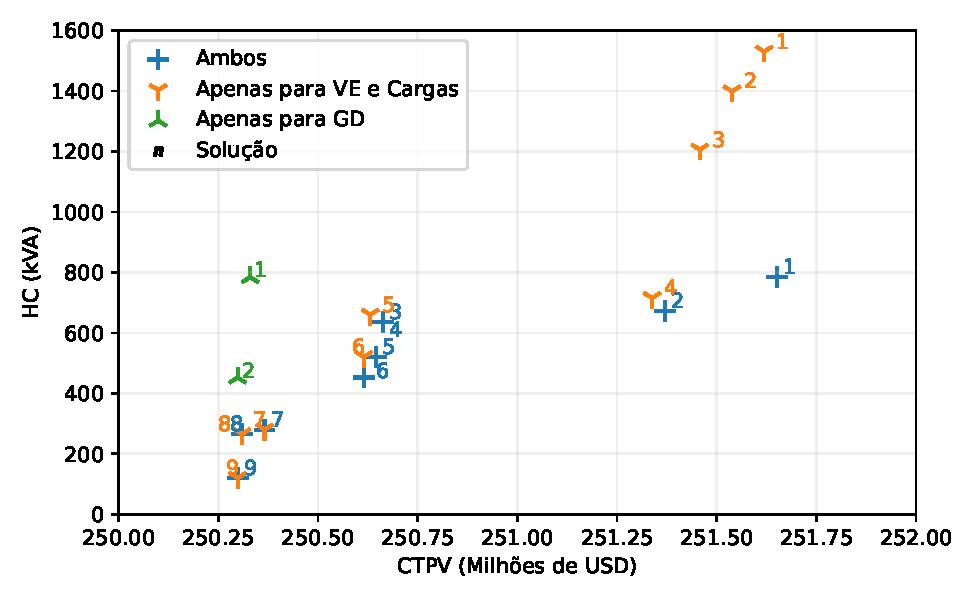
\includegraphics[width=0.8\textwidth]{cap4/resultados/24_pareto.pdf}\\
    \label{fig:24_pareto}
\end{figure}


Vale destacar como planejar o sistema de distribuição apenas visando minimizar os custos, impacta diretamente no valor de \ac{HC} do sistema de distribuição. Visando apenas custos para o cenários de ambos, chega-se a um valor de 120 kVA a um custo de 250,3 milhões de dólares. Já visando apenas \ac{HC} para o cenários de ambos, chega-se a um valor de 784 kVA a um custo de 251,65 milhões de dólares, aproximadamente uma relação de 492 kVA por milhão de dólares, em um investimento que na casa de um quarto de bilhão de dólares.


A discrepância de quantidades de soluções entre o cenário de apenas geradores distribuídos e os outros levantaram o questionamento da causa desta diferença. Inicialmente, foram testadas alterações no valor de pico das cargas e valores de cenários de carregamentos, porém, não foi encontrada nenhuma evidência que essas alterações impactaram diretamente a diferença de soluções entre os cenários avaliados. Desta forma, optou-se por investigar a fundo as soluções encontradas. A seguir, soluções pertinentes são discutidas para identificar o que impacta a relação entre \ac{HC} e $c^{TPV}$, bem como a quantidade de soluções encontradas.

\newpage
\subsection{Resultados para o sistema de 24 nós -- Apenas geração distribuída}

Como foram obtidas apenas duas soluções para o caso de apenas geração distribuída, facilmente podemos avaliar a diferença entre cada solução. Na figura \ref{fig:24_gen}, observa-se que esta diferença está relacionada apenas à localização de um gerador eólico instalado no sistema no último estágio.
Esta é a primeira evidência que a localização de geradores distribuídos podem impactar no valor de \ac{HC} em sistemas de distribuição. Porém, vale destacar que não houve diferença entre a localização de geradores distribuídos que podem ser operados pela empresa de distribuição (apresentados na figura \ref{fig:24_gen} como geradores convencionais "CX"), apenas geradores distribuídos renováveis impactaram no valor de \ac{HC} neste cenário.

Esta observação é enfatizada ao verificarmos na literatura todos os trabalhos que discutem como controlar e integrar estes tipos de geradores em sistemas de distribuição, conforme visto na seção \ref{hc_review_control_dg}.

Destaca-se também que esta observação ocorreu apenas após a adição dos cenários de geradores renováveis distribuídos (através do parâmetro $\alpha^{RW}$) no modelo base de otimização. Sem as mudanças propostas por este trabalho no modelo de \citeonline{MunozDelgado2015}, esta observação não se torna possível e o modelo retorna apenas uma solução de \ac{HC} para este cenário.
\newpage

\begin{figure}[H]
 	\centering
    \caption{24 nós -- Solução 1 e 2 para o caso de apenas GD. Em vermelho: apenas solução 1. Em verde: apenas solução 2.}
    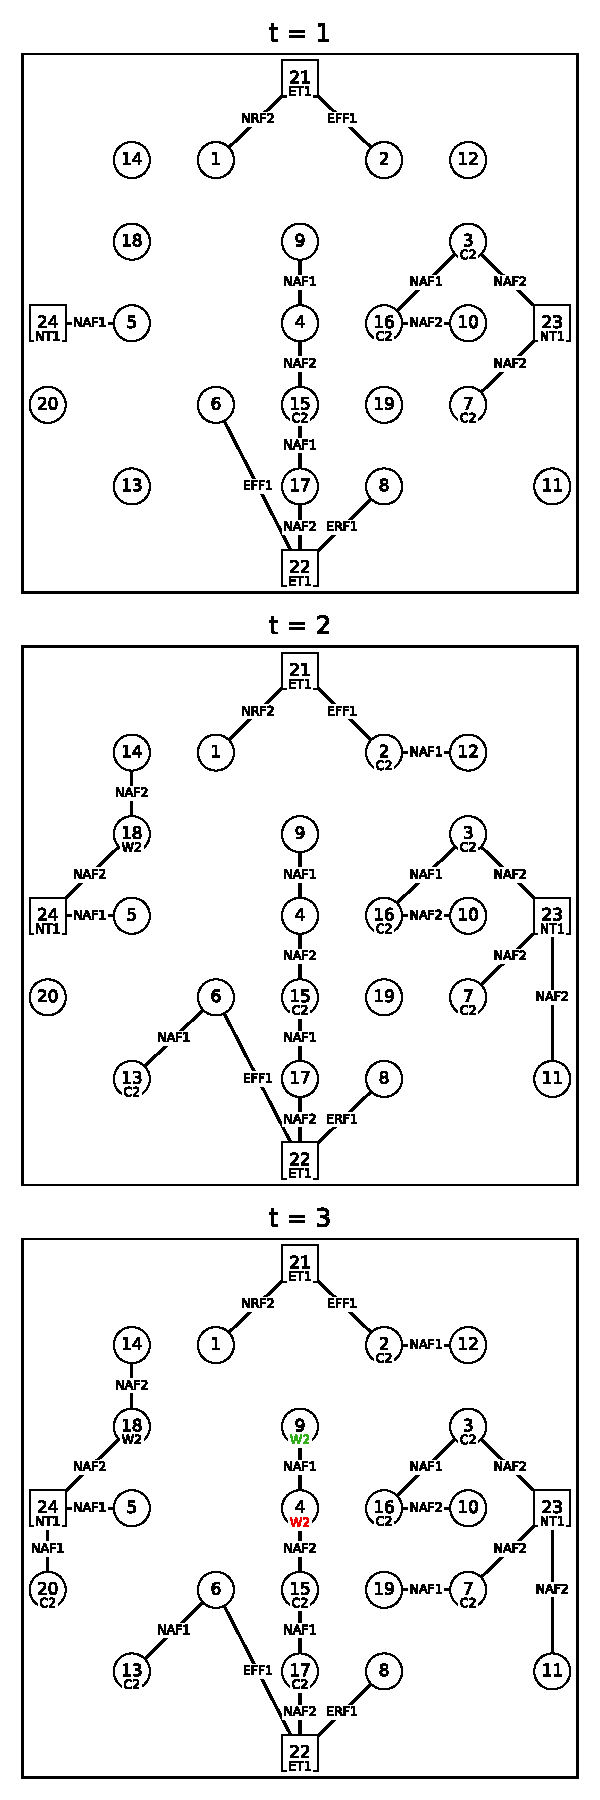
\includegraphics[width=0.5\textwidth]{cap4/resultados/24_gen2.pdf}\\
    \label{fig:24_gen}
\end{figure}

\subsection{Resultados para o sistema de 24 nós -- Apenas veículos elétricos ou cargas}

Neste cenário foram selecionadas quatro soluções (solução 1, 4, 5 e 9) das nove encontradas para serem avaliadas. Estas soluções foram escolhidas pois representam as maiores diferenças entre os valores de \ac{HC} e $c^{TPV}$.

Na figura \ref{fig:24_ev1_4}, é possível observar o que causou a diferença entre a solução 1 (1,3 MVA e 251,62 milhões de dólares) e a solução 4 (0,715 MVA e 251,34 milhões de dólares). Observa-se que esta diferença ocorre devido ao tipo de transformador utilizado em cada solução no nó 23. A solução 1 utiliza a alternativa 2 (um transformador de 15 MVA), já a solução 4 utiliza a alternativa 1 (um transformador de 12 MVA).

Note que mesmo com 3 MVA de capacidade do transformador instalado, a diferença entre os valores de \ac{HC} não foi 3 MVA. Isto ocorre, devido aos limites operacionais de tensão e carregamento do sistema e não apenas devido aos limites de capacidade do transformador e das linhas.  Isto demonstra que estes limites operacionais podem ser violados caso uma carga maior que as encontradas no valor de \ac{HC} deste cenário for instalada no sistema.

Outra característica importante é que não foram observadas mudanças de topologia entre estas duas soluções. O que evidencia que a escolha de transformadores causa um maior impacto no valor de \ac{HC} neste cenário do que mudanças topológicas.

Já na figura \ref{fig:24_ev5_9}, é possível observar o que causou a diferença entre a solução 5 (0,66 MVA e 250,63 milhões de dólares) e a solução 9 (0,12 MVA e 250,3 milhões de dólares). Nestas soluções já observam-se mudanças topológicas significativas, porém, também  observam-se diferentes alternativas de transformadores nó 23, bem como o estágio  de instalação de geradores distribuídos nos nós 2 e 15.

Curiosamente, entre a solução 1 (de maior \ac{HC} e maior $c^{TPV}$) e a solução 9 (de menor \ac{HC} e menor $c^{TPV}$), não há nenhuma diferença topológica. Entretanto, há diferença na construção de uma nova subestação com a instalação de um novo transformador no nó 22 e a alternativa da linha que liga os nós 15 e 17. Isto novamente evidencia que a escolha das alternativas de investimento tem um maior impacto do que a topologia do sistema.

\newpage
\begin{figure}[H]
 	\centering
    \caption{24 nós -- Solução 1 e 4 para o caso de apenas EV. Em vermelho: apenas solução 1. Em verde: apenas solução 4.}
    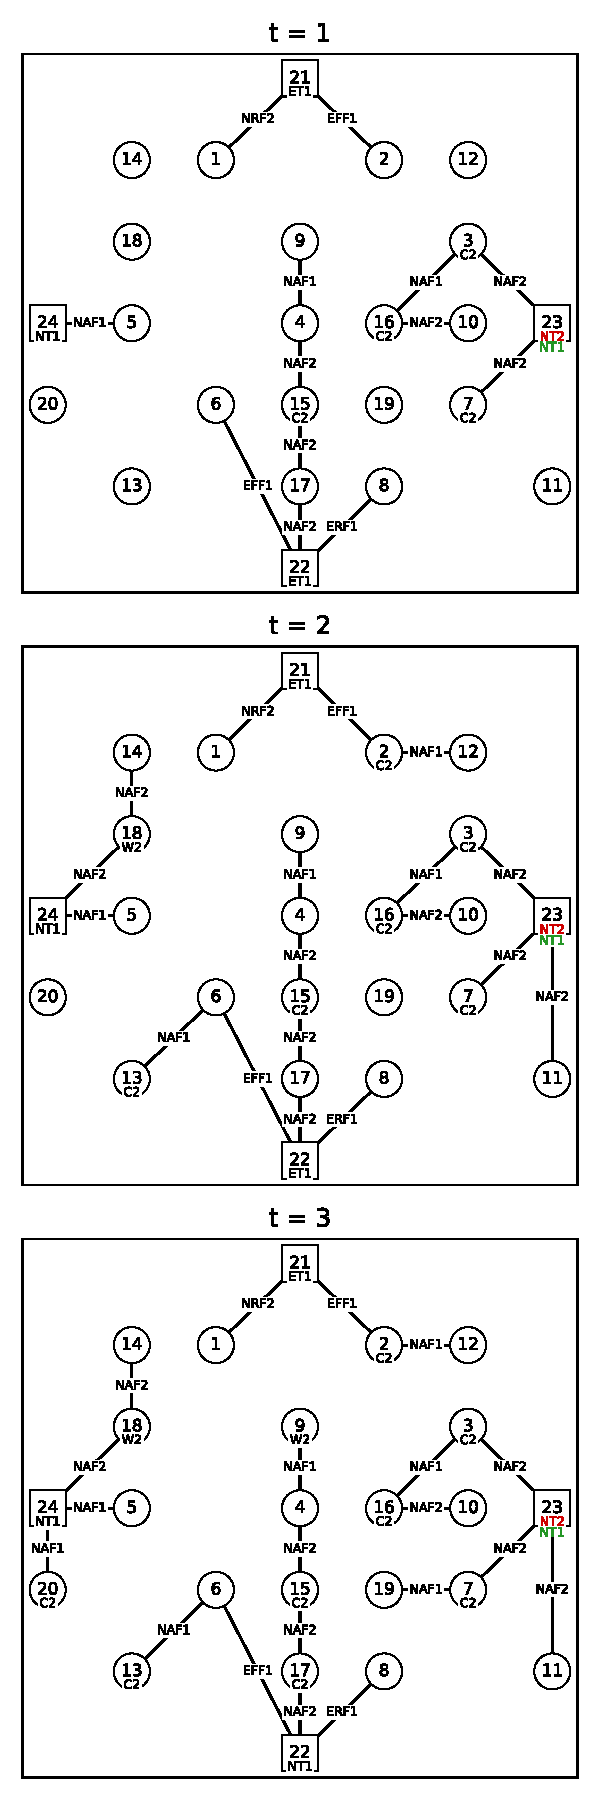
\includegraphics[width=0.5\textwidth]{cap4/resultados/24_ev1.pdf}\\
    \label{fig:24_ev1_4}
\end{figure}

\begin{figure}[H]%
\centering
\caption{24 nós -- Solução 5 e 9 para o caso de apenas EV. (a) Solução 5. (b) Solução 9.}
\begin{tabular}{cc}
    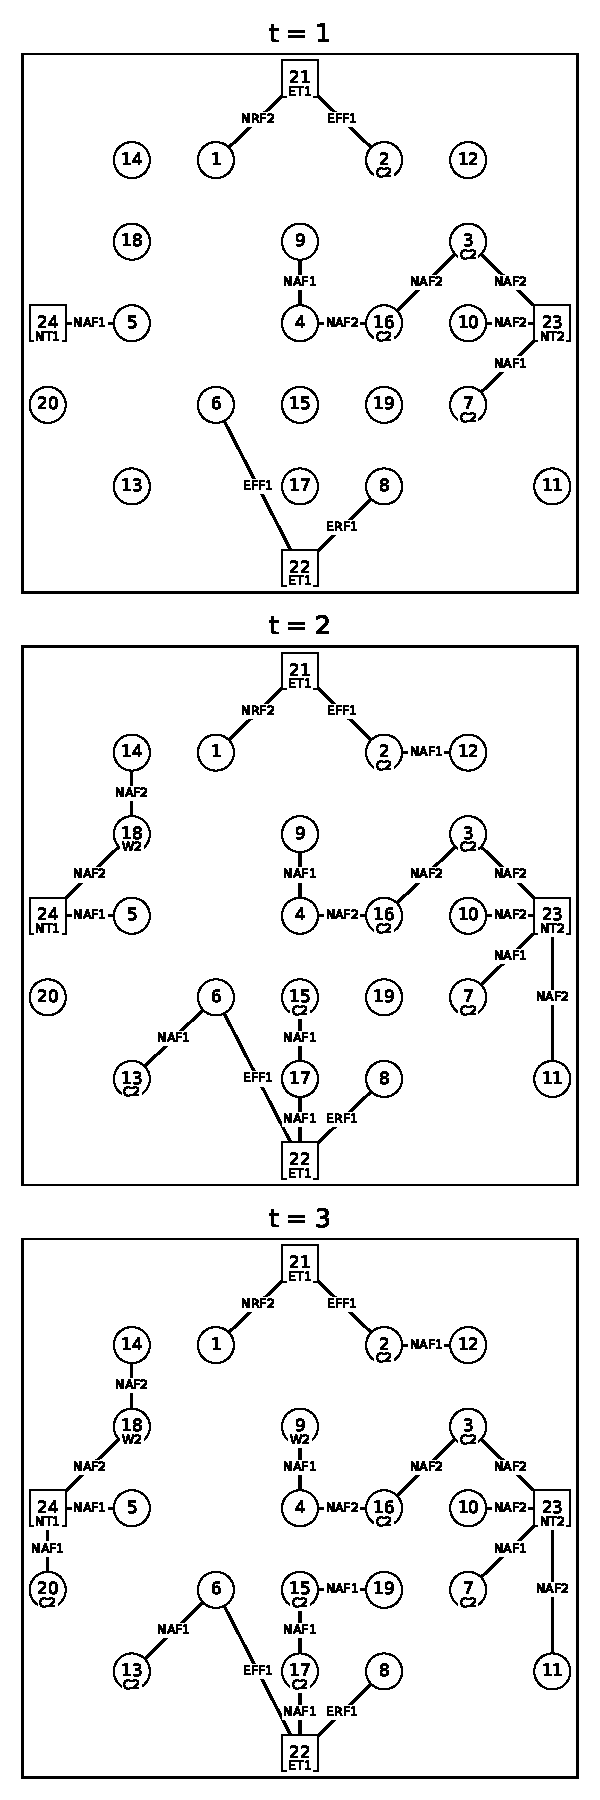
\includegraphics[width=0.49\columnwidth]{cap4/resultados/24_ev5.pdf} & 
    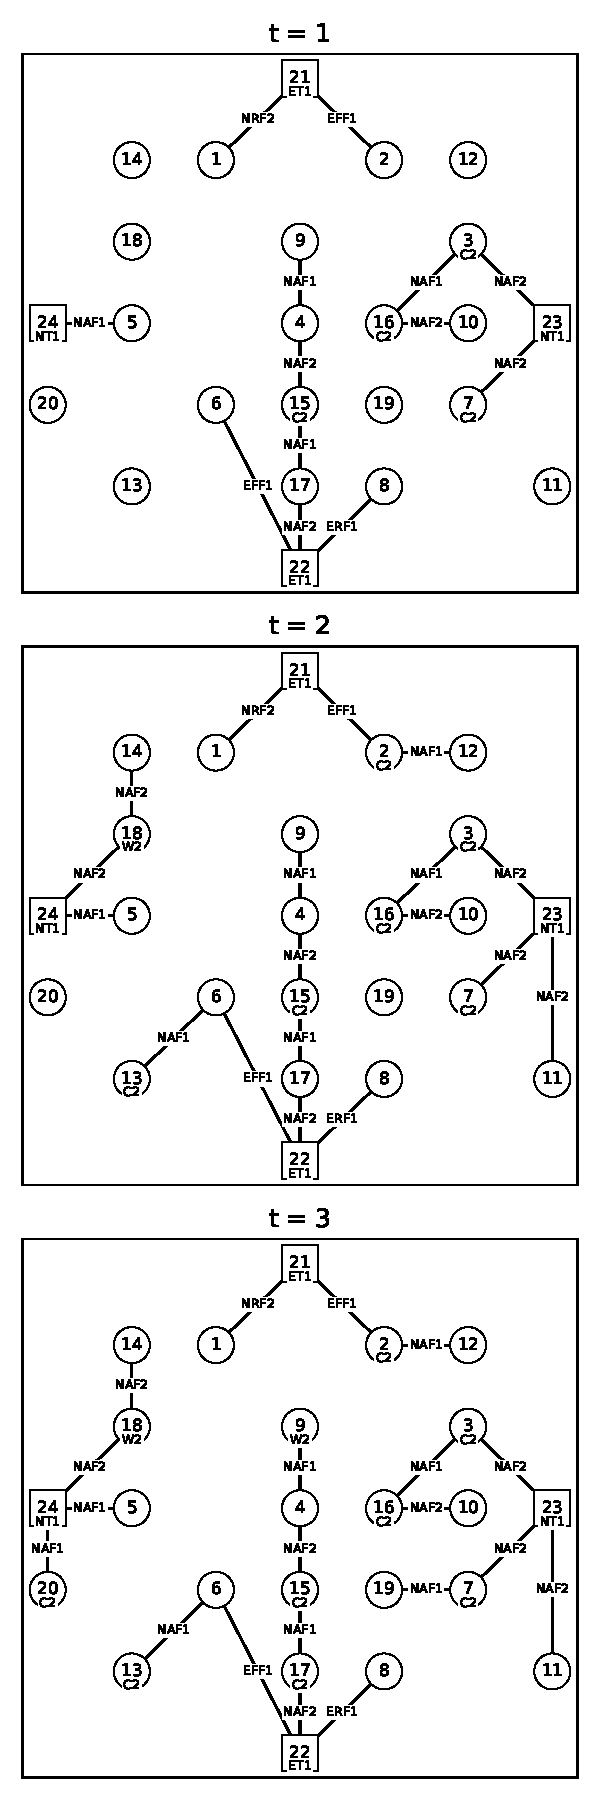
\includegraphics[width=0.49\columnwidth]{cap4/resultados/24_ev9.pdf} \\
    (a) & (b) 
\end{tabular}
\label{fig:24_ev5_9}
\end{figure}

\newpage
\subsection{Resultados para o sistema de 24 nós -- Ambos}

Neste cenário foram selecionadas três soluções (solução 1, 6 e 9) das nove encontradas para serem avaliadas. Estas soluções foram escolhidas pois representam as maiores diferenças entre os valores de \ac{HC} e $c^{TPV}$.


Na figura \ref{fig:24_both1_6} são apresentadas as soluções 1 (784 kVA e 251,65 milhões de dólares) e 6 (452,2 kVA e 250,61 milhões de dólares). Já na figura \ref{fig:24_both9} é apresentada a solução 9 (120 kVA e 250,3 milhões de dólares).

Observa-se uma grande diferença topológica entre as soluções 1 e 6, mas não entre 1 e 9. Indicando mais uma vez que neste sistema mudanças de topologias causam impactos menores, tanto no valor de \ac{HC} quanto nos custos do \ac{PESD}. Curiosamente, há uma grande diferença topológica entre as soluções 6 e 9 também, indicando que mudanças topológicas atuam como um ajuste fino nas soluções encontradas.

Por outro lado, observa-se também grandes diferenças nas opções de investimentos em todas as três soluções apresentadas. Destaca-se a localização do gerador eólico nos nós 4 e 9 nas soluções 1 e 9, bem como a construção de uma nova subestação no nó 22 com a instalação de um novo transformador nas mesmas soluções 1 e 9.

\subsection{Análise entre cenários para o sistema de 24 nós}

Pode-se observar que as diferenças topológicas não impactam tanto quanto as diferenças entre opções de investimentos, principalmente nas soluções em que há diferenças na instalação ou não de novos transformadores e construção de subestações. Entretanto, as soluções observadas neste sistema apresentam fortes evidências que as mudanças topológicas se comportam como um ajuste fino da localização da solução na fronteira de Pareto.

Foi observado também que há um impacto considerável no valor de \ac{HC} dependendo da localização de geradores distribuídos renováveis. Porém, esta localização pouco impacta nos custos do \ac{PESD}. Logo, uma análise mais profunda da localização e da operação destes geradores podem trazer benefícios consideráveis para o valor de \ac{HC} do sistema de distribuição.

Observou-se também que mesmo obtendo-se poucas soluções para o cenário de apenas geradores distribuídos, estas soluções apresentam uma seleção de alternativas e topologia muito semelhante às que são observadas nos outros cenários. O que indica que quanto mais soluções são observadas no cenário apenas de geradores distribuídos, muito mais soluções podem ser observadas nos outros cenários de análise.

\newpage
\begin{figure}[H]%
\centering
\caption{24 nós -- Solução 1 e 6 para o caso de ambos. (a) Solução 1. (b) Solução 6.}
\begin{tabular}{cc}
    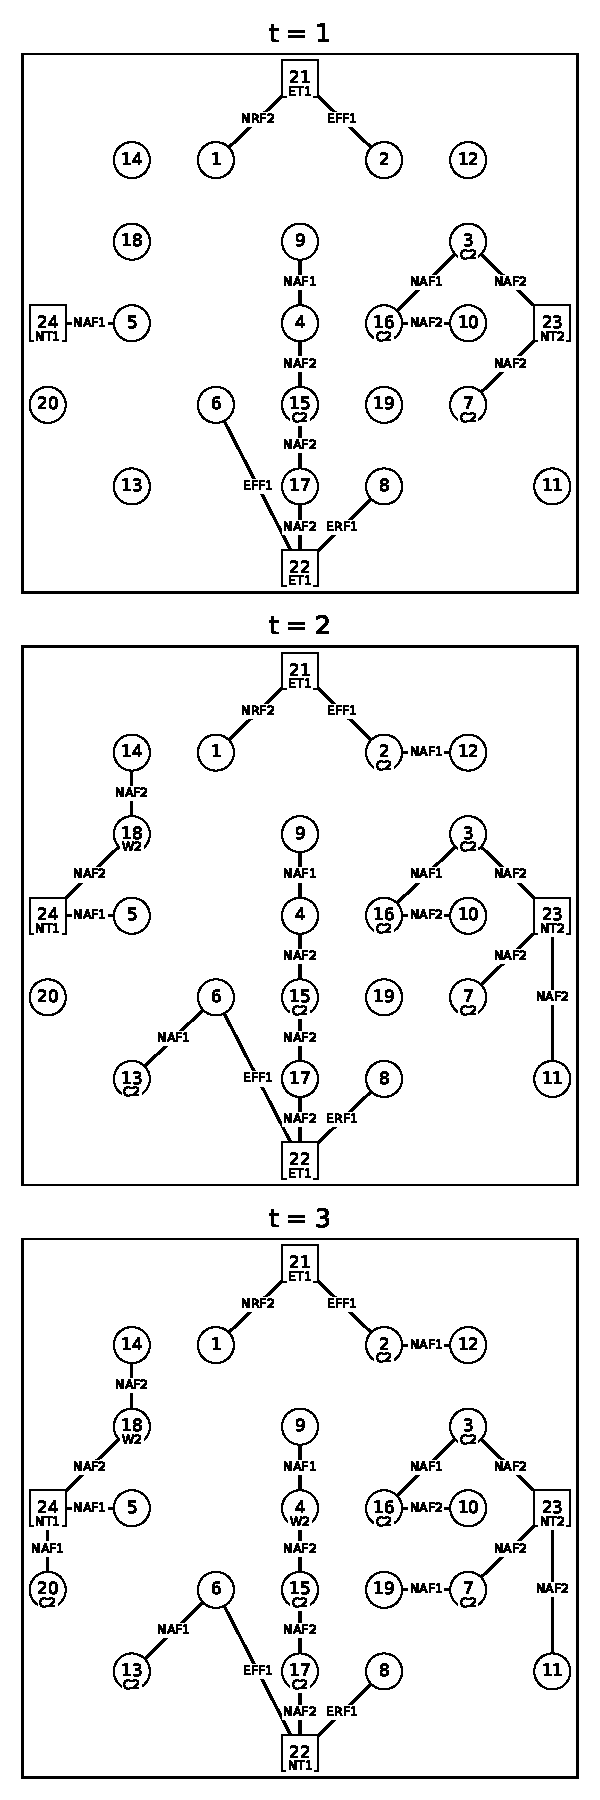
\includegraphics[width=0.49\columnwidth]{cap4/resultados/24_both1.pdf} & 
    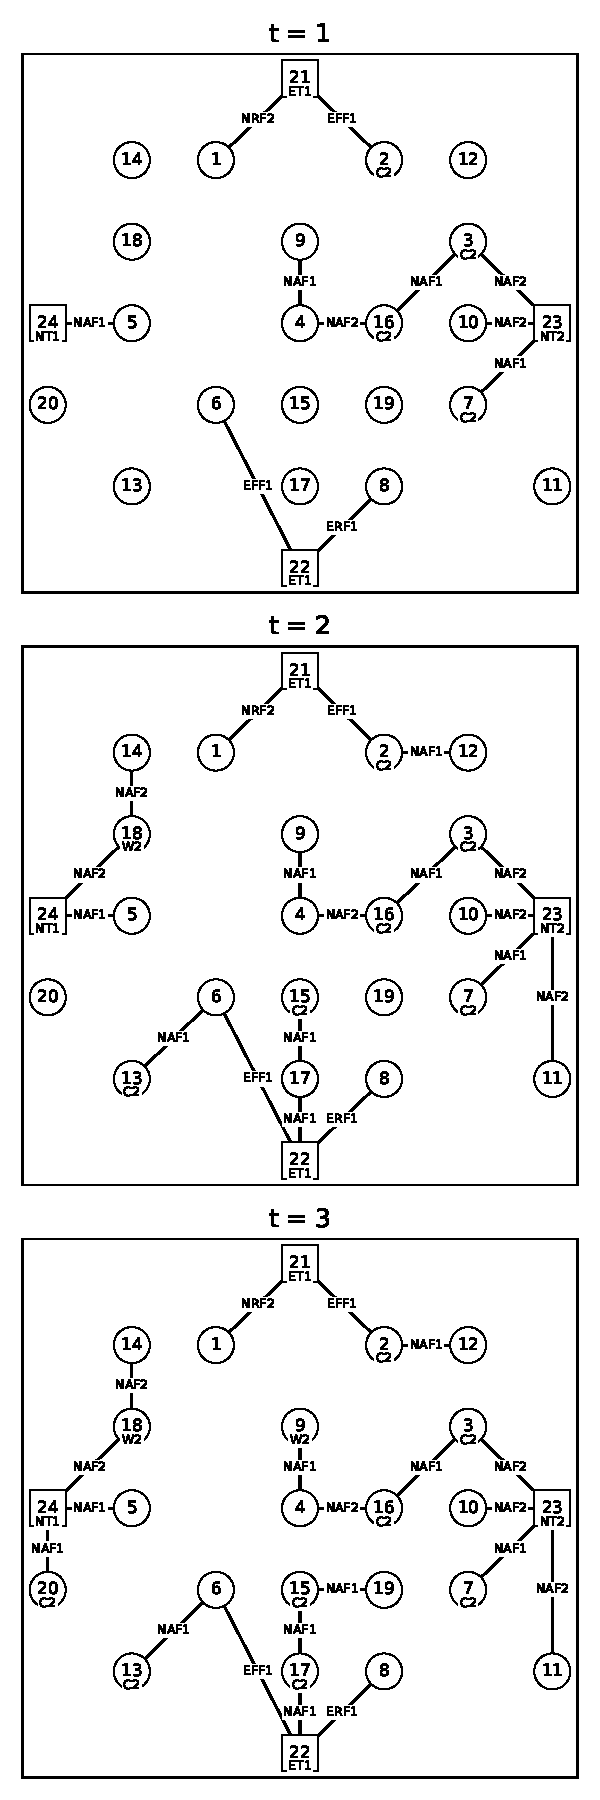
\includegraphics[width=0.49\columnwidth]{cap4/resultados/24_both6.pdf} \\
    (a) & (b) 
\end{tabular}
\label{fig:24_both1_6}
\end{figure}

\begin{figure}[H]
 	\centering
    \caption{24 nós -- Solução 9 para o caso de ambos.}
    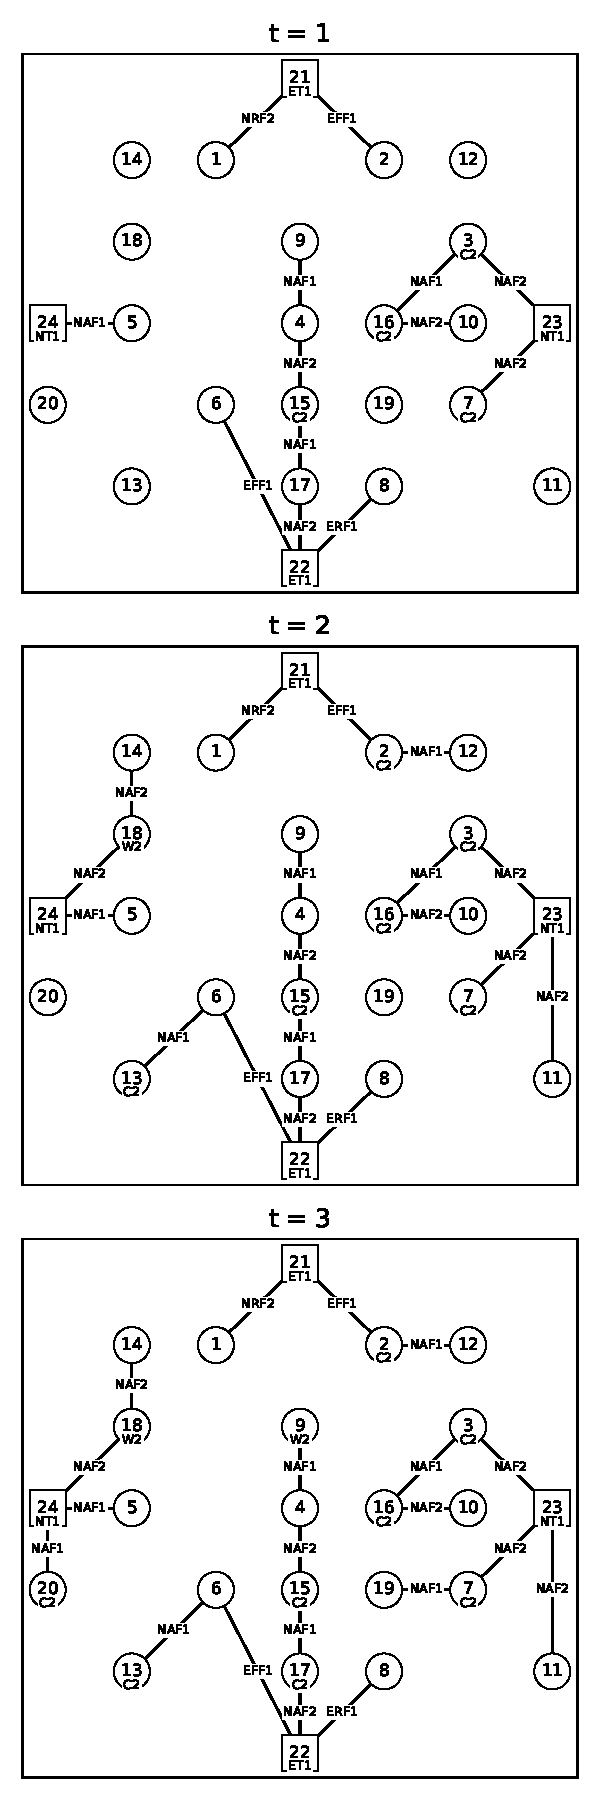
\includegraphics[width=0.5\textwidth]{cap4/resultados/24_both9.pdf}\\
    \label{fig:24_both9}
\end{figure}

\section{Resultados para o sistema de 54 nós}

Para o sistema de 54 nós, também foram realizados três cenários de análise, o primeiro considerando apenas o \ac{HC} para geração distribuída, o segundo considerando o \ac{HC} apenas para veículos elétricos ou novas cargas e o terceiro considerando ambos. Estes cenários foram avaliados com a alteração dos parâmetros $\alpha^{HC}$.

Ao executar a resolução do modelo bi-objetivo para apenas geração distribuída, obteve-se apenas uma solução, com valor de 128,8 kVA de \ac{HC} e 450,86 milhões de dólares de $c^{TPV}$. Por outro lado, tanto para apenas veículos elétricos ou novas cargas quanto para ambos (veículos elétricos e geradores distribuídos), foram obtidas quatro soluções entre 67,8 kVA a 32,3 kVA de \ac{HC} e 458,24 milhões de dólares a 450,86 milhões de dólares de $c^{TPV}$. A figura \ref{fig:54_pareto} apresenta as soluções obtidas, as opções de investimentos podem ser vistas também no Apêndice \ref{sec:tab54}. Vale salientar que o cenário de apenas veículos elétricos ou novas cargas e o cenário para ambos (geração distribuída e veículos elétricos ou novas cargas) apresentaram as mesmas soluções, tanto de investimentos quanto de topologia do sistema.
\vspace{-0.5cm}
\begin{figure}[h]
 	\centering
    \caption{54 nós -- Soluções encontradas.}
    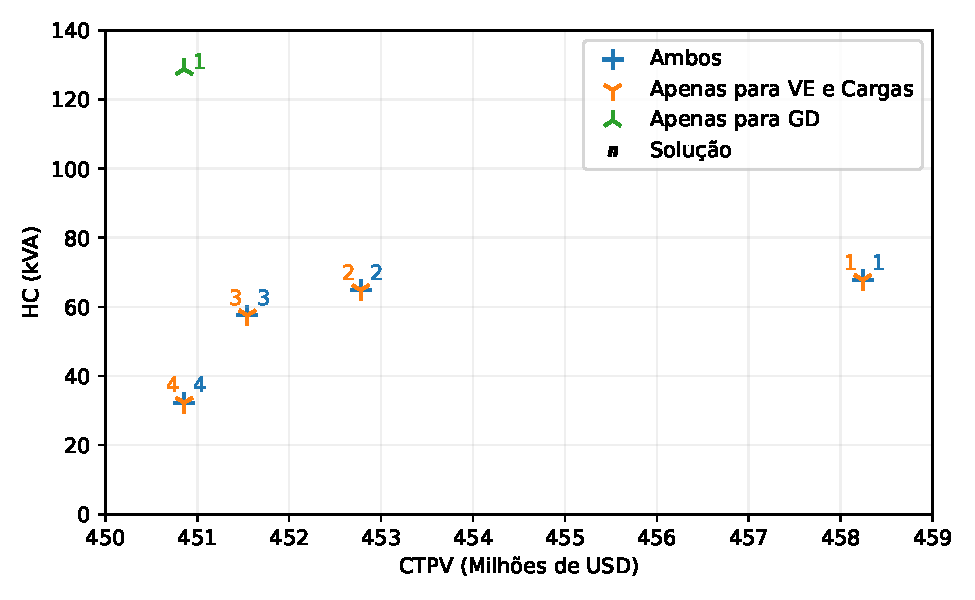
\includegraphics[width=0.8\textwidth]{cap4/resultados/54_pareto.pdf}\\
    \label{fig:54_pareto}
\end{figure}
\vspace{-0.8cm}

É possível observar o mesmo comportamento das soluções de uma relação direta entre o custo total do \ac{PESD} com o valor de \ac{HC} estimado para o sistema. Observa-se também uma relação de aproximadamente 4,81 kVA por milhão de dólares (no caso de ambos), um valor muito menor do qual foi encontrado do sistema de 24 nós, indicando que cada sistema de distribuição a ser planejado possui suas próprias características, porém, seguindo um mesmo comportamento de solução. 


Novamente foi observada uma discrepância de quantidades de soluções entre o cenário de apenas geradores distribuídos e os outros. Novamente, foram testadas alterações no valor de pico das cargas e valores de cenários de carregamentos, porém, não foi encontrada nenhuma evidência que essas alterações impactaram diretamente a diferença de soluções entre os cenários avaliados.

\subsection{Resultados para o sistema de 54 nós -- Apenas geração distribuída}
\vspace{-0.2cm}
Como foram obtidas apenas uma solução para o caso de apenas geração distribuída, facilmente pode-se avaliá-la. Na figura \ref{fig:54_gen}, observa-se que todas as barras que podem receber geradores distribuídos, foram instalados geradores distribuídos, inclusive, mais de um gerador distribuído por nó como, por exemplo, no nó 15, no qual foi instalado um gerador eólico e um gerador convencional. Isto indica que a solução encontrada busca manter controlada a operação do sistema de distribuição, pois apenas os geradores convencionais possuem a capacidade de controle de despacho.
Observa-se também que mesmo com todos os geradores instalados, novas subestações foram necessárias e que isso não causou tantos impactos no valor final de $c^{TPV}$ em relação às soluções encontradas nos outros cenários.
\vspace{-0.2cm}
\begin{figure}[H]
 	\centering
    \caption{54 nós -- Solução 1 para o caso de apenas geração.}
    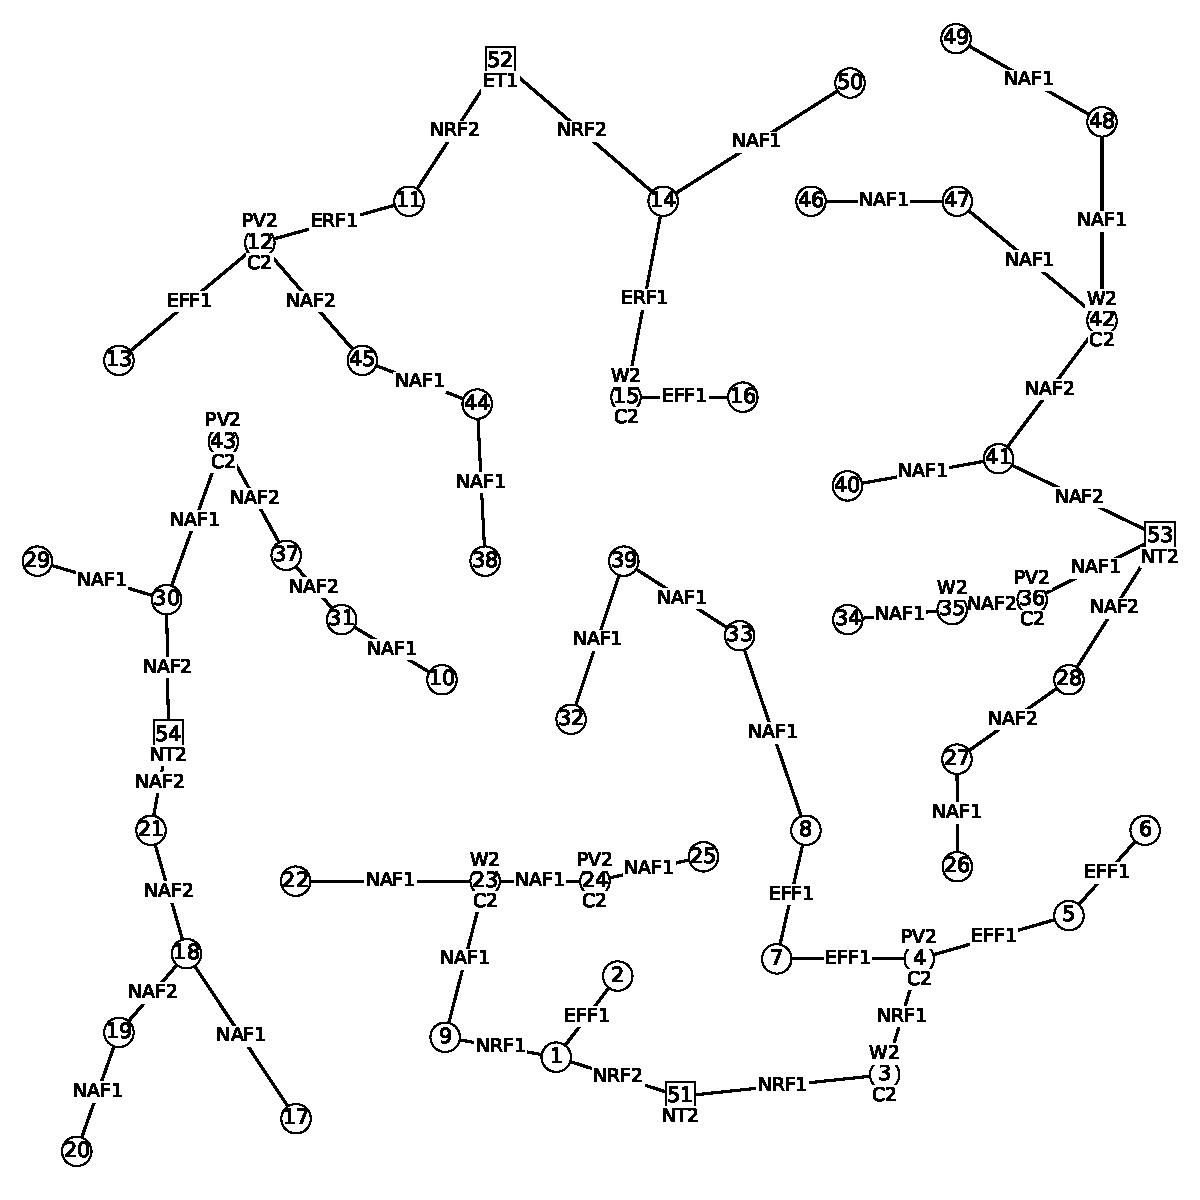
\includegraphics[width=1.02\textwidth]{cap4/resultados/54_bus_gen.pdf}\\
    \label{fig:54_gen}
\end{figure}


\subsection{Resultados para o sistema de 54 nós -- Ambos e apenas veículos elétricos ou cargas}

Como o cenários de ambos e apenas veículos elétricos ou cargas apresentaram as mesmas soluções, elas são apresentadas juntas nas figuras de \ref{fig:54_both1} a \ref{fig:54_both4}.

Observa-se na solução 1 (figura \ref{fig:54_both1}) que todos os nós que podem ter geradores distribuídos instalados, tiveram geradores instalados e que os mesmos geradores, subestações e transformadores foram instalados da mesma forma que a solução para apenas geração distribuída. Por outro lado, há uma diferença significativa na topologia do sistema de distribuição, isso ocorre devido a presença das novas cargas no sistema de distribuição no cenário de ambos e apenas veículos elétricos ou cargas que não ocorrem no cenário de apenas geradores elétricos.

\begin{figure}[h]
 	\centering
    \caption{54 nós -- Solução 1 para o caso de ambos e apenas veículos elétricos ou cargas.}
    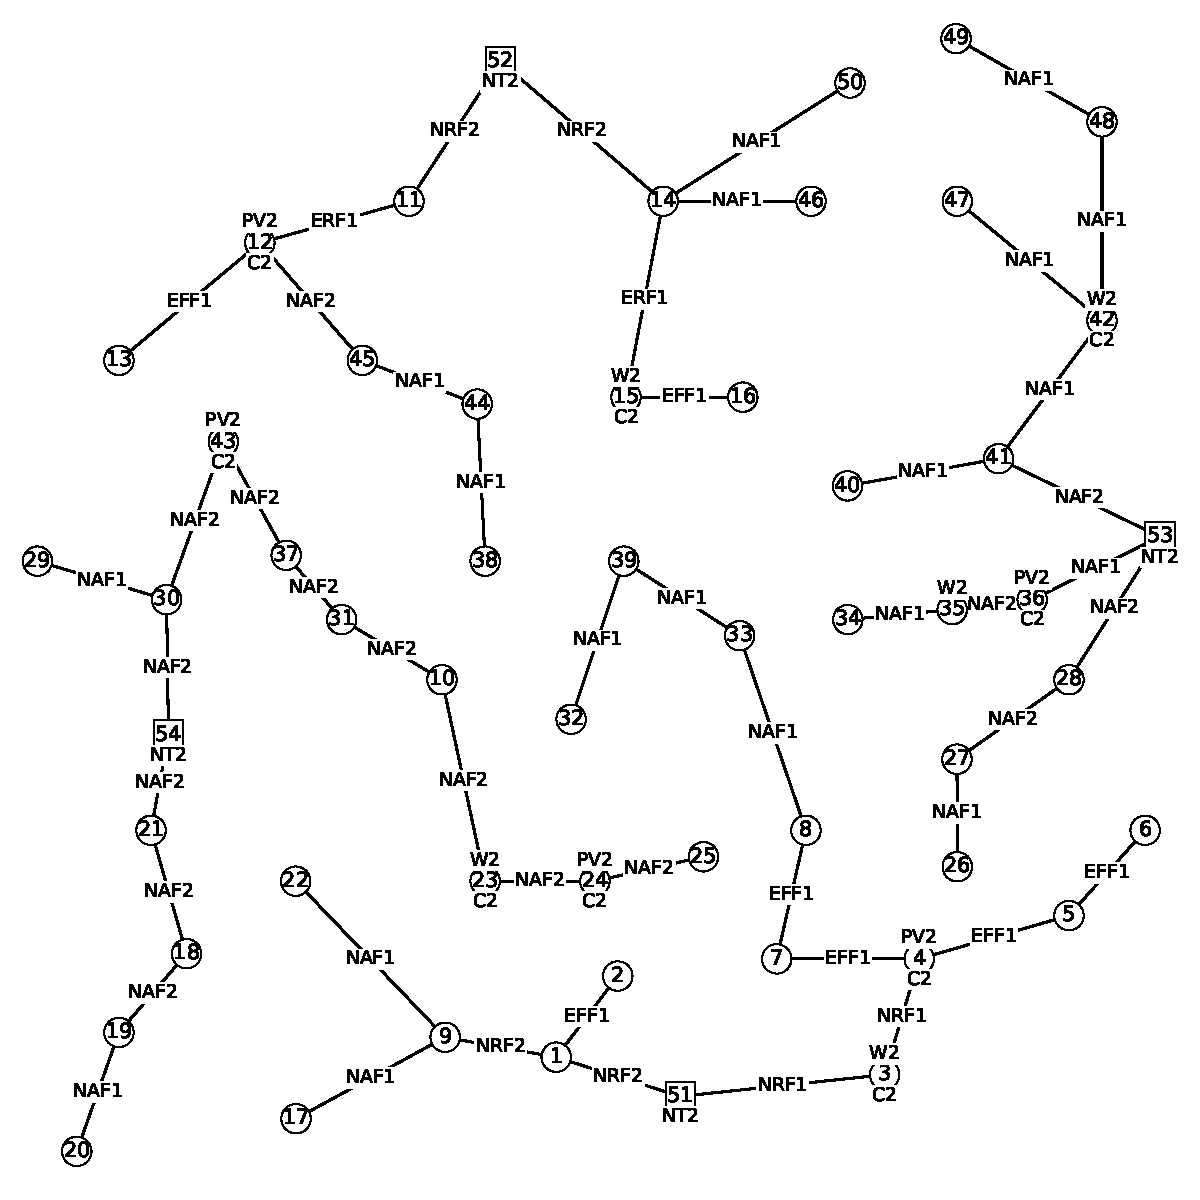
\includegraphics[width=1.02\textwidth]{cap4/resultados/54_bus_both1.pdf}\\
    \label{fig:54_both1}
\end{figure}


Já na solução 2 (figura \ref{fig:54_both2}) observou-se também que todos os nós que podem ter geradores tiveram estes instalados da mesma forma que as outras soluções apresentadas anteriormente. Por outro lado, com uma diferença significativa na topologia do sistema de distribuição. Curiosamente, apenas a topologia e a operação dos geradores convencionais foram diferentes entre as duas soluções. Este comportamento é observado também na solução 3 (figura \ref{fig:54_both3}), que não apresenta diferença entre os investimentos que não sejam relacionados a topologia e cabos de alimentadores.
\begin{figure}[h]
 	\centering
    \caption{54 nós -- Solução 2 para o caso de ambos e apenas veículos elétricos ou cargas.}
    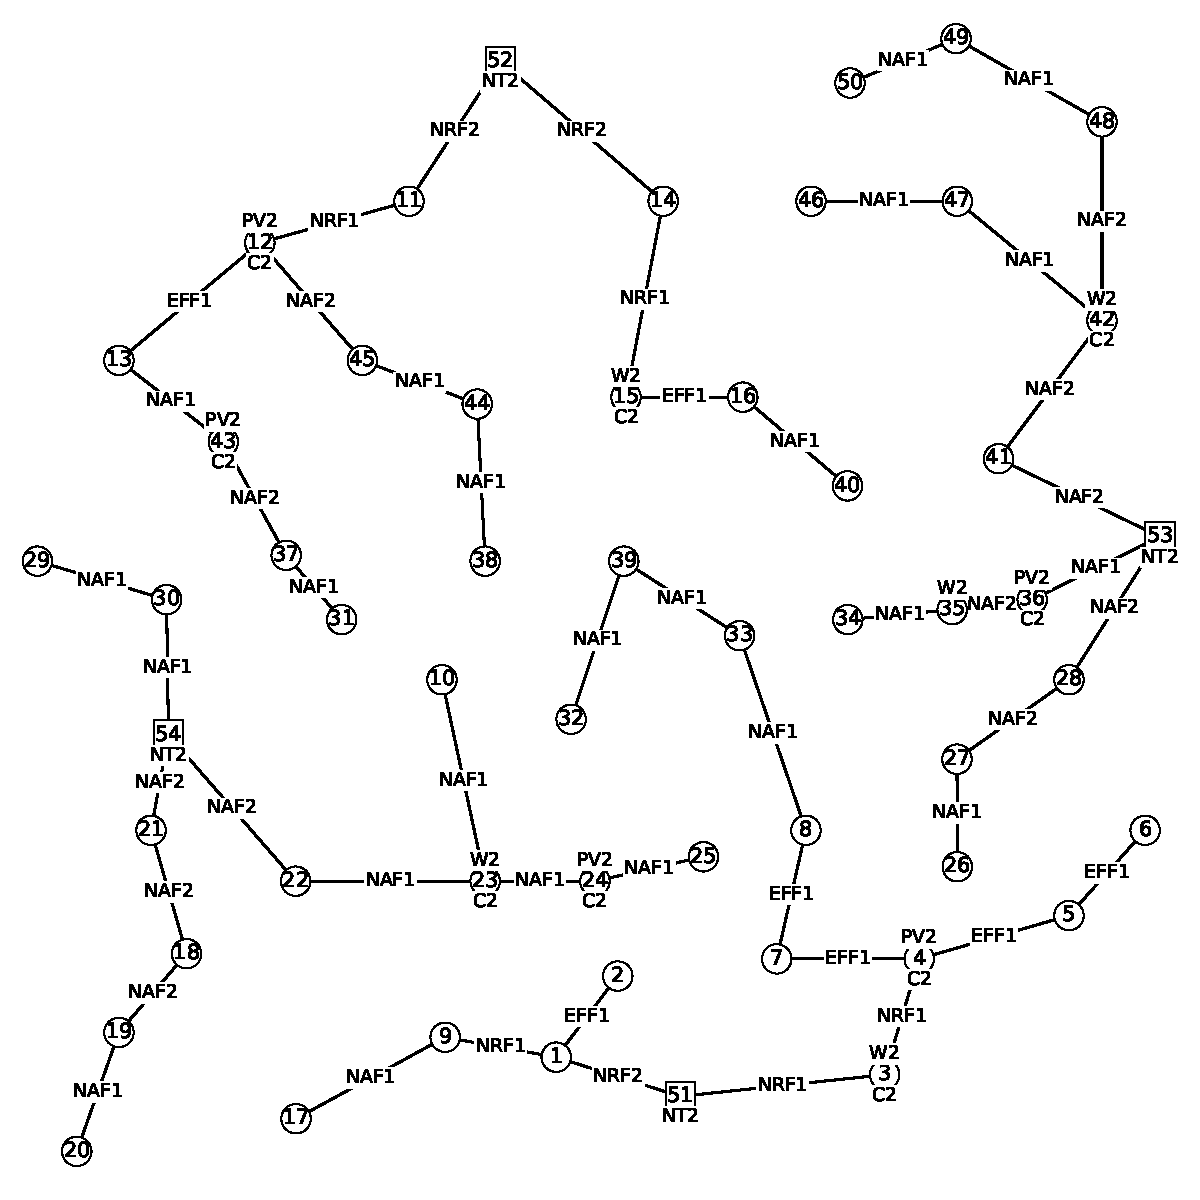
\includegraphics[width=1.02\textwidth]{cap4/resultados/54_bus_both2.pdf}\\
    \label{fig:54_both2}
\end{figure}

\begin{figure}[ht]
 	\centering
    \caption{54 nós -- Solução 3 para o caso de ambos e apenas veículos elétricos ou cargas.}
    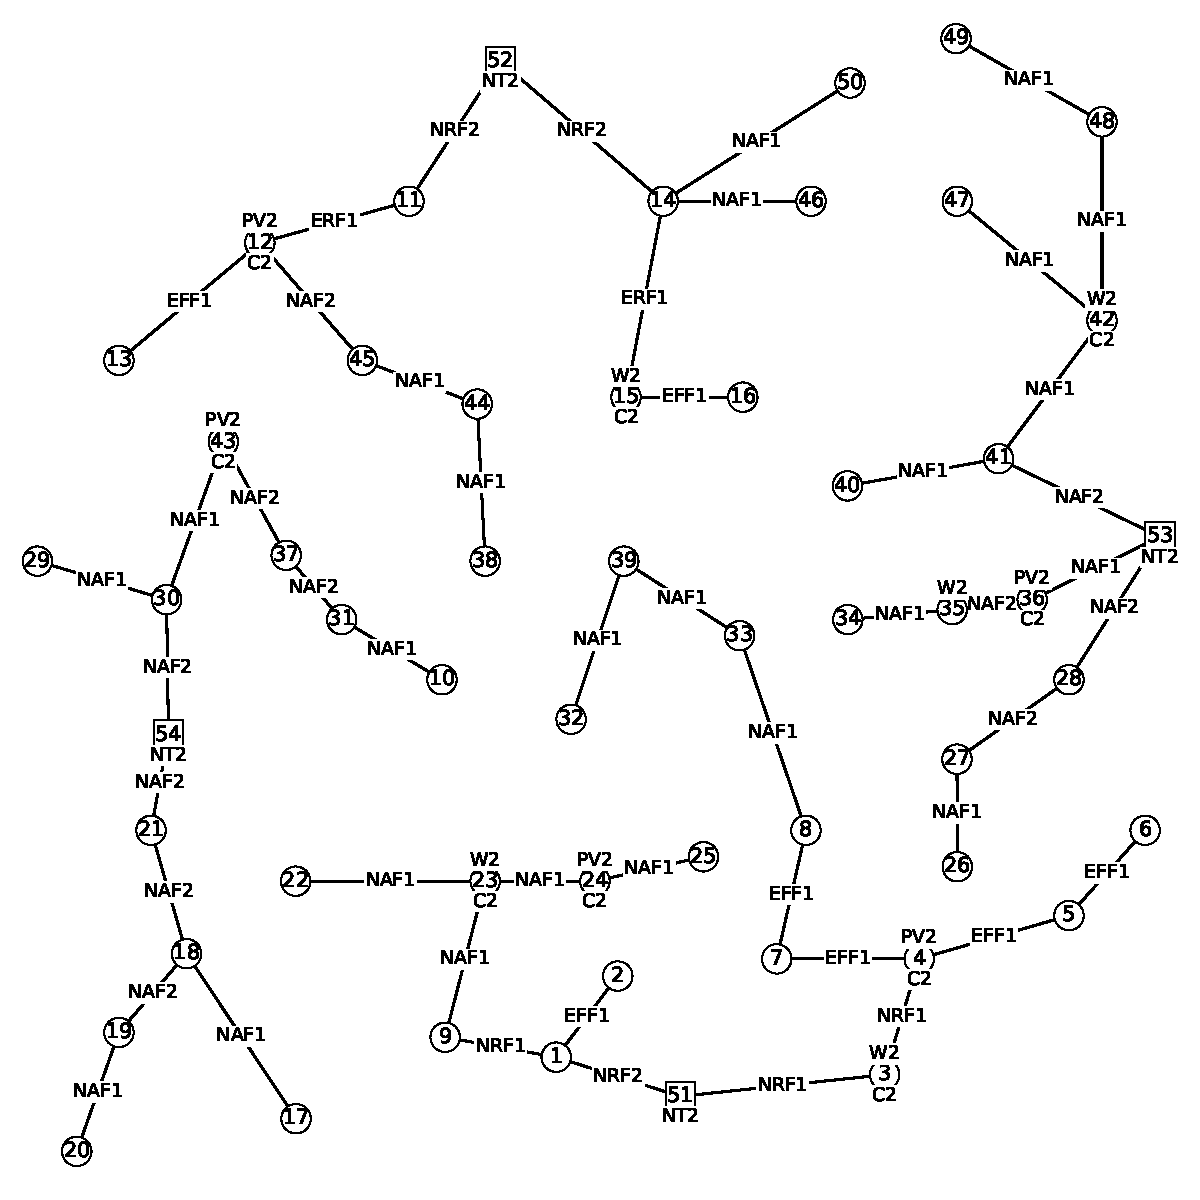
\includegraphics[width=1.02\textwidth]{cap4/resultados/54_bus_both3.pdf}\\
    \label{fig:54_both3}
\end{figure}

Observa-se, porém, que na solução 4 (figura \ref{fig:54_both4}) há uma diferença nas opções de investimentos que não a topologia/cabos. Nesta solução, não foi feito o investimento de construção da subestação e instalação de um novo transformador nó 52, o que impactou diretamente os valores de \ac{HC} e $c^{TPV}$. 

\subsection{Análise entre cenários para o sistema de 54 nós}

Diferente do que foi observado no sistema de 24 nós, neste, ocorreu um impacto significativo da topologia do sistema, visto que não foram encontradas outras soluções com outras opções de investimentos que poderiam gerar uma solução dominante durante as buscas dos pontos da fronteira de Pareto. Entretanto, as soluções encontradas para este sistema também indicam que o ajuste da topologia do sistema de distribuição se comporta como um ajuste fino dos pontos na fronteira de Pareto, visto que a mudança de transformador no nó 52 causa um grande impacto, tanto no valor de \ac{HC} quanto no valor de $c^{TPV}$.

Observou-se também, que nós com geradores renováveis também tiveram geradores convencionais instalados nos mesmos. Isto pode indicar que este sistema precisa de uma certa "estabilidade"\; na geração distribuída para manter os níveis de tensão adequados, bem como a capacidade de \ac{HC}.

Por fim, destaca-se a diferença de valor de \ac{HC} entre a solução para apenas geradores distribuídos e as soluções para ambos e apenas veículos elétricos ou cargas. Isto indica que este sistema é muito mais receptivo a instalação de novos geradores distribuídos do que novas cargas.

\begin{figure}[h]
 	\centering
    \caption{54 nós -- Solução 4 para o caso de ambos e apenas veículos elétricos ou cargas.}
    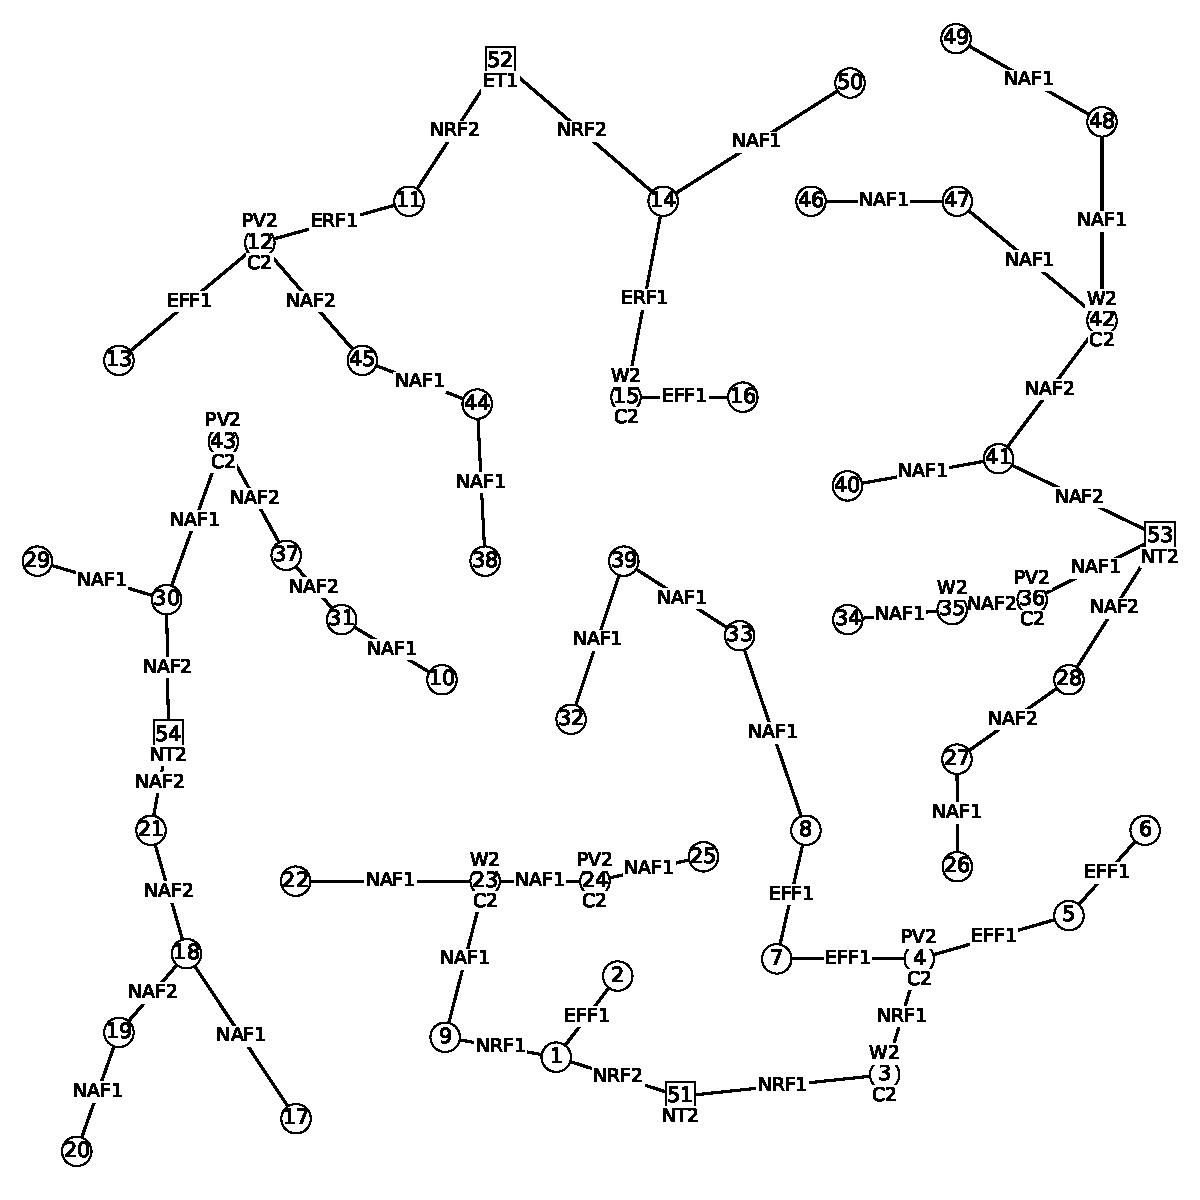
\includegraphics[width=1.02\textwidth]{cap4/resultados/54_bus_both4.pdf}\\
    \label{fig:54_both4}
\end{figure}

\newpage
\section{Resultados para o sistema de 138 nós}

Para o sistema de 138 nós, também foram realizados três cenários de análise, o primeiro considerando apenas o \ac{HC} para geração distribuída, o segundo considerando o \ac{HC} apenas para veículos elétricos ou novas cargas e o terceiro considerando ambos. Estes cenários foram avaliados com a alteração dos parâmetros $\alpha^{HC}$.

Diferente de todos os outros resultados obtidos, no sistema de 138 nós, foram encontradas 10 soluções para caso de apenas geração distribuída, 44 soluções para o caso de apenas veículos elétricos ou novas cargas e 34 soluções para o caso de ambos. Todas as opções de investimentos podem ser vistas no Apêndice \ref{sec:tab54}, as soluções foram enumeradas de forma que a solução com menor índice indica maior \ac{HC} e a solução com maior índice indica menor \ac{HC}, conforme a implementação apresentada na figura \ref{fig:method}.

A figura  \ref{fig:54_pareto} apresenta os pontos da fronteira de Pareto obtidas durante a resolução do modelo bi-objetivo em todos os três cenários de análise. Note que para o cenário de apenas geração distribuída o \ac{HC} varia entre 78,055 kVA ($c^{TPV}$ de 118,94 milhões de dólares) e  17,815 kVA ( $c^{TPV}$ de 117,07 milhões de dólares). Já para o caso de apenas veículos elétricos ou novas cargas o \ac{HC} varia entre 118,555 kVA ($c^{TPV}$ de 120,52 milhões de dólares) e 7,141 kVA ($c^{TPV}$ de 117,07 milhões de dólares). No caso de ambos o \ac{HC} varia entre 68,905 kVA ($c^{TPV}$ de 122,35 milhões de dólares) e 7,143 kVA ($c^{TPV}$ de 117,07 milhões de dólares).

\begin{figure}[h]
 	\centering
    \caption{138 nós -- Soluções encontradas.}
    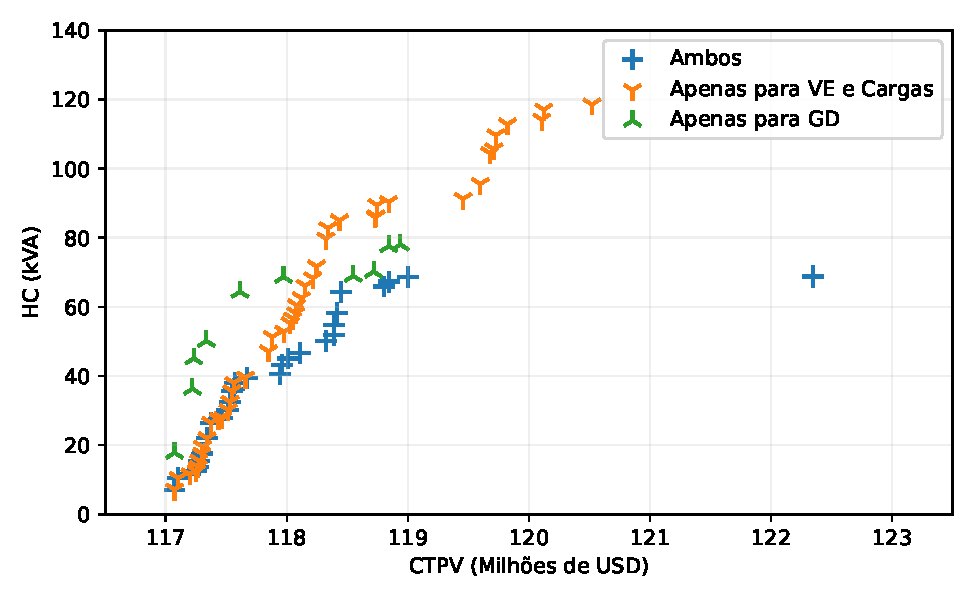
\includegraphics[width=0.8\textwidth]{cap4/resultados/138_pareto.pdf}\\
    \label{fig:138_pareto}
\end{figure}

É possível observar o mesmo comportamento das soluções de uma relação direta entre o custo total do \ac{PESD} com o valor de \ac{HC} estimado para o sistema. Observa-se também uma relação de aproximadamente 11,69 kVA por milhão de dólares, um valor muito menor do qual foi encontrado do sistema de 24 nós, porém na mesma magnitude do sistema de 54 nós. Isto reforça a hipótese de que cada sistema de distribuição a ser planejado possui suas próprias características, porém, seguindo um mesmo comportamento de solução. 

Apesar de ter sido obtido mais soluções para o caso de apenas geradores distribuídos, a mesma discrepância de quantidades de soluções entre o cenário de apenas geradores distribuídos e os outros foi observada. Novamente, foram testadas alterações no valor de pico das cargas e valores de cenários de carregamentos, porém, não foi encontrada nenhuma evidência que essas alterações impactaram diretamente a diferença de soluções entre os cenários avaliados.

Durante a escrita desta tese, não foi identificado uma boa forma de representar graficamente todas as diferenças entre as soluções e ainda assim apresentar o sistema final obtido através das soluções de investimentos encontradas em sistemas de distribuição grandes como o de 138 nós. Exemplos de trabalhos similares também sofrem do mesmo problema. Desta forma, a discussão dos resultados é apresentada pontuando investimentos e mudanças de topologias relevantes identificadas nas soluções. Caso seja necessário mais detalhes sobre as soluções, o autor indica a inspeção das tabelas no Apêndice \ref{sec:tab54} e o código fonte implementado, disponível em \cite{modelocomHC}.

\subsection{Resultados para o sistema de 138 nós -- Apenas geração distribuída}

No sistema de 138 nós observou-se que a melhoria de \ac{HC} ocorre através da instalação de geradores distribuídos e da topologia do sistema de distribuição. Não houve alterações nas opções de transformadores, nem a construção de novas subestações, sendo a construção da subestação e a instalação de transformador nos nós 138, 137 e 136 foram necessárias em todas as soluções encontradas.

Com relação a diferença de geradores distribuídos, a diferença entra a solução com maior \ac{HC} (solução 1) e a solução com menor \ac{HC} (solução 10) se dá pela alternativa de investimento nos geradores distribuídos convencionais dos nós 94 e 53 e pela instalação ou não de um gerador eólico (alternativa 2) no nó 52. Nos nós 94 e 53, a solução 1 opta por instalar geradores distribuídos convencionais com maior potência (alternativa 2) do que a solução 10. Já a solução 10 opta por instalar o gerador eólico no nó 52. Isto pode indicar que a operação dos geradores convencionais de maior capacidade trazem maior flexibilidade na operação, possibilitando um maior valor de \ac{HC}, enquanto a inserção de geradores renováveis sem um devido controle de sua operação pode prejudicar o valor de \ac{HC}, mesmo que reduzam os custos de operação.

Já analisando a mudança topológica entre a solução com maior \ac{HC} (solução 1) e a solução com menor \ac{HC} (solução 10), é possível observar que são sistemas diferentes, mas que possuem semelhanças. Isso é observado já que apenas quatro alimentadores são diferentes entre as soluções. A solução 1 interliga os nós: 104 ao 105, 44 ao 45, 111 ao 112, 114 ao 123, todos utilizando a alternativa 1. A solução 10 interliga os nós: 43 ao 52, 28 ao 29, 108 ao 138, 113 ao 114, todos utilizando a alternativa 1.

Durante a avaliação das soluções, foi observado apenas um caso em que a escolha de um condutor com mais ampacidade resultou em uma mudança de valor de \ac{HC}. Isto ocorre na diferença entre as soluções 7 e 8 no alimentador que interliga o nó 43 ao 52. Entretanto, a diferença entre as duas soluções também apresenta diferenças entre instalação de geradores convencionais e de topologia do sistema planejado.

De modo geral, observou-se que os geradores despacháveis melhoraram o valor de \ac{HC} neste sistema com este cenário de análise, bem como mudanças topológicas.

\subsection{Resultados para o sistema de 138 nós -- Apenas veículos elétricos e cargas}

No caso de apenas veículos elétricos e cargas as diferenças são mais evidentes, pois há tanto instalação geradores distribuídos diferentes, topologias diferentes, construção de novas subestações, instalação de novos transformadores e instalação de condutores com maior ampacidade.

Em relação aos geradores distribuídos instalados e comparando a solução com maior \ac{HC} (solução 1) e a solução com menor \ac{HC} (solução 44), é possível observar que possuem a mesma quantidade de geradores instalados. Porém, a solução 1 instala um gerador convencional com maior potência no nó 94 e outro no nó 133, enquanto a solução 10 instala um gerador convencional com menor potência no nó 94 e um gerador eólico no nó 52.

Destaca-se também a escolha da solução 1 de se construir novas subestações e transformadores nos nós 136 e 137 em relação a não opção pelos mesmos na solução 44. Por fim, vale observar que as topologias também são diferentes, porém com grande semelhanças entre eles, visto que apenas 7 alimentadores são diferentes entre a solução 1 e a solução 44.

Dentre as 44 soluções, pode-se observar que apenas 11 investimentos para aumentar a ampacidade de linhas foram são escolhidos se for avaliado a diferença entre as soluções par a par. A maioria destes investimentos ocorrem no alimentador que liga o nó 105 ao 122. Curiosamente, o observou-se também a escolha de se reduzir a ampacidade de um alimentador (mesmo com melhoria de \ac{HC}), especialmente entre os nós 43 e 52. Esta última observação pode ser explicada pela redução de corrente que flui pelos nós 43 e 52 com a mudança de topologia.

Da mesma forma que anteriormente, observou-se que geradores despacháveis melhoraram o valor de HC neste sistema com este cenário de análise, bem como mudanças topológicas.

\subsection{Resultados para o sistema de 138 nós -- Ambos}

Para o caso de ambos ocorrem as mesmas diferenças observados para o caso de apenas veículos elétricos e cargas, porém, é possível observar mais soluções que apresentam a decisão de aumentar a ampacidade de um dos condutores para elevar o valor de \ac{HC} em relação a solução vizinha. Neste caso de análise, observou-se a instalação de geradores distribuídos diferentes, topologias diferentes, construção de novas subestações, instalação de novos transformadores e instalação de condutores com maior ampacidade.

Da mesma forma que o caso de apenas veículos elétricos e cargas, a solução com maior \ac{HC} (solução 1) apresenta a escolha de mais geradores distribuídos convencionais, enquanto a solução com menor \ac{HC} (solução 34) opta por instalar mais geradores eólicos. Observou-se também a opção de se construir novas subestações e instalar novos transformadores nos nós 136 e 137 na solução 1 que não é observada na solução 34.

A decisão de aumentar a ampacidade das linhas foi mais evidente neste cenário de análise, principalmente nas primeiras soluções. Foi observado que a opção por condutores de maior ampacidade ocorreu como um ajuste ainda mais fino do valor de \ac{HC}, além do ajuste feito pelas mudanças de topologia.

E mais uma vez se observou que geradores despacháveis melhoraram o valor de HC neste sistema com este cenário de análise, bem como mudanças topológicas.



\subsection{Análise entre cenários para o sistema de 138 nós}

Neste sistema foi observado que ocorrem cenários em que mudanças topológicas causam um aumento significativo no valor do \ac{HC} enquanto há cenários em que as outras opções de investimentos causam maiores impactos neste indicador. Como este sistema é maior, levanta-se a hipótese de que quanto maior o sistema, maior a quantidade de soluções que podem ser encontradas na fronteira de Pareto. Por outro lado, é possível que esta quantidade maior de soluções seja possível devido às características topológicas e das opções de investimentos.

Observou-se que os geradores renováveis impactaram negativamente o valor de \ac{HC}. Esta observação pode ser explicada pois no modelo implementado, os geradores renováveis não são despacháveis, o que causa um "consumo" da banda de \ac{HC} disponível em uma determinada solução. Outra hipótese que pode ser levantada é que este sistema precisa de uma certa "estabilidade"\; na geração distribuída para manter os níveis de tensão adequados, bem como a capacidade de \ac{HC}.

Por fim, destaca-se a diferença de valor de \ac{HC} entre a solução para apenas geradores distribuídos e as soluções para ambos e apenas veículos elétricos ou cargas. Isto indica que este sistema é muito mais receptivo a instalação de novas cargas e veículos elétricos.

% \section{Estimativa da capacidade de hospedagem}

% A estimativa do valor de HC do sistema de distribuição é realizada em conjunto com o PESD e os valores de contribuição de cada nó para o valor total do HC em cada estágio pode ser vista na figura \ref{fig:result_hc}.

% Observa-se que o valor de HC vai aumentando com o passar dos estágios e que nem todos os nós do sistema contribuem para o valor de HC. Isto é esperado para os nós que não estão conectados ao sistema de distribuição, por outro lado, no segundo e terceiro estágio os nós 12 e 13 não contribuem para o valor de HC mesmo estando conectados e possuindo cargas. Isto nos leva a crer que há múltiplas soluções dos HC locais, porém o valor total estimado permanece o mesmo. Desta forma, observa-se que a estimativa do HC local não deve ser considerada como rígida, sendo necessário a avaliação do HC a cada solicitação de nova instalação de geradores distribuídos.


% A partir dos resultados de investimentos e custos, no qual foi observado uma grande quantidade de alocação dos geradores distribuídos operados pela empresa distribuidora, esperava-se que isto impactaria no valor de HC estimado. Porém, como estes geradores distribuídos são despacháveis o aumento da injeção de outros geradores distribuídos (estes já não controlados pela empresa distribuidora) são compensados com a redução de injeção de potência dos que já foram instalados. Este comportamento nos leva a perceber que os geradores distribuídos já alocados podem acabar em desuso com o crescimento da injeção de novos geradores distribuídos. 

% Desta forma, observa-se que há um típico comportamento de risco associado à instalação dos geradores distribuídos durante a expansão do sistema de distribuição, que envolve alocá-los para que, em um futuro próximo, talvez sejam subutilizados e não contribuindo para uma redução significativa no valor presente líquido dos custos totais, visto que a maior parte provém da expectativa de menor custos com produção de energia. 

% Por outro lado, a alocação destes geradores distribuídos operados pela empresa distribuidora, fornecem um certa segurança em relação a operação do sistema de distribuição. Visto que é garantido que todos os requisitos operacionais serão atendidos, com ou sem novos geradores distribuídos instalados.

% Vale observar que no modelo utilizado não está prevista a instalação de sistemas de armazenamento de energia, dos quais podem contribuir tanto para a operação do sistema de distribuição, quanto para a melhoria do valor de HC observado nos resultados obtidos.

% Levanta-se o questionamento sobre o HC de estações de veículos elétricos que, do ponto de vista do modelo utilizado, se comportam apenas como novas cargas no sistema de distribuição e poderá ser implementado neste modelo futuramente. Talvez, com a integração destas novas cargas o risco de desuso de geradores distribuídos instalados durante a expansão do sistema de distribuição pode deixar de se tornar relevante, principalmente pelo comportamento de grandes picos e vales na demanda que estas cargas causam.

% Por fim, não é possível deixar de observar que o modelo proposto já indica uma otimização multi-objetivo que relaciona os custos com o PESD com a melhoria do valor de HC. Espera-se que no futuro sejam implementadas rotinas para expressar esta relação. Por outro lado, a integração tanto do HC de estações de veículos elétricos quanto a alocação de sistemas de armazenamento de energia também podem auxiliar na identificação desta relação.


% ---
% Finaliza a parte no bookmark do PDF, para que se inicie o bookmark na raiz


\bookmarksetup{startatroot}% 
% ---

% ---
% Conclusão
% ---
\chapter{Considerações finais}
\label{consideraçao}

Nesta tese, apresentou-se uma proposta de modelo que integra o \ac{PESD} com a
estimativa do valor de \ac{HC} de recursos energéticos distribuídos. Este modelo
foi desenvolvido a partir de uma formulação baseada no modelo proposto por
\citeonline{MunozDelgado2015}.

Esta proposta baseou-se nos conceitos de \ac{HC} encontrados na literatura para
introduzi-lo no contexto de \ac{PESD}, formulando um novo modelo com uma nova
função objetivo e restrições a fim de estimar o valor de \ac{HC}. Esta
formulação envolve um espelhamento das restrições do comportamento do sistema de
distribuição, permitindo simular a presença de novos geradores distribuídos. A
integração entre o modelo de \ac{PESD} e o modelo proposto de \ac{HC} é
realizada através de uma modelagem bi-objetiva, que é solucionada utilizando a
união dos métodos de $\epsilon$-restrito e otimização hierárquica.

A eficácia da proposta é demonstrada através dos resultados obtidos a partir da
aplicação do modelo proposto em três sistemas teste baseados nos encontrados na
literatura. Os resultados apontam que o modelo bi-objetivo proposto resulta em
várias opções de decisões de investimento que demonstram a concorrência entre os
objetivos de redução de custos com sistema planejado e aumento do valor de
\ac{HC}. Além disso, foram observados que mudanças topológicas podem causar
impactos no valor de \ac{HC}, e que a relação entre os custos com o \ac{PESD} e
valor de \ac{HC} devem ser investigados caso-a-caso.

A principal contribuição dos modelos apresentados é a integração dos modelos
clássicos de \ac{PESD} com a estimativa do valor de \ac{HC}. A partir destes
modelos, também foi possível observar quantativamente a relação entre os custos
com o \ac{PESD} e a melhoria do valor de \ac{HC}. Observou-se que, até o momento
da escrita desta tese, não foram encontrados trabalhos acadêmicos similares que
demonstraram essa relação nem uma forma de estima-la.

Entretanto, há diversas oportunidades de melhoria no modelo apresentado nesta
tese. Um exemplo de melhoria seria a adição de uma análise mais estatística do
comportamento de cargas, geração renovável e avaliação do \ac{HC}, bem como a
inserção da modelagem de sistemas de armazenamento de energia durante a expansão
do sistema de distribuição. Portanto, na forma apresentada nesta tese, os
modelos devem ser interpretados como uma avaliação inicial de possíveis
soluções. Recomenda-se então que estas oportunidades sejam investigadas em
trabalhos futuros.

A seguir são apresentadas as publicações realizadas desde o início do doutorado.


\section{Publicações realizadas}

\noindent FILHO, SERGIO A. DE MORAIS ; \textbf{MONTEIRO, FELIPE M. DOS S.} ; VIEIRA, JOSE CARLOS M. ; ASADA, EDUARDO N. ; BICZKOWSKI, MAURICIO . Impact Index for Allocating Transportable Energy Storage Systems in Power Distribution Networks. In: \textit{2019 IEEE Milan PowerTech}, IEEE, 2019. 

\noindent Disponível em:
https://ieeexplore.ieee.org/document/8810675/

\vspace{1cm}
\noindent DE SOUZA, JONAS V. ; MOMESSO, ANTONIO E. C. ; \textbf{MONTEIRO, FELIPE M. DOS S.} ; OTTO, RODRIGO B. ; ASADA, EDUARDO N. . Intelligent Management of Battery System for Energy Arbitrage. In: \textit{2019 IEEE Milan PowerTech}, IEEE, 2019. 

\noindent Disponível em:
https://ieeexplore.ieee.org/document/8810805

\vspace{1cm}
\noindent  DE SOUZA, JONAS V. ; FARIA, WANDRY R. ; \textbf{MONTEIRO, FELIPE M. DOS S.} ; OTTO, RODRIGO B. ; BICZKOWSKI, MAURICIO ; ASADA, EDUARDO N. . Battery Energy Storage System Allocation in Distribution Systems for Power Loss and Operational Costs Reduction. In: \textit{2019 IEEE PES Innovative Smart Grid Technologies Conference Latin America (ISGT Latin America)}, IEEE, 2019.

\noindent Disponível em:
https://ieeexplore.ieee.org/document/8810805

\newpage
\vspace{1cm}
\noindent \textbf{MONTEIRO, F. M. DOS S.}; SOUZA. J. V.; ASADA, E. Multistage Distribution System Expansion Planning with many Alternatives of Conductors. In: \textit{ 2020 IEEE Power \& Energy Society General Meeting (PESGM)}. IEEE, 2020. 

\noindent Disponível em: https://ieeexplore.ieee.org/document/9281945

\vspace{1cm}
\noindent SOUZA. J. V.; \textbf{MONTEIRO, F. M. DOS S.};  ASADA, E.; OTTO, R.; BICZKOWSKI, M. Management of an Electrical Storage System for Joint Energy Arbitrage and Improvement of Voltage Profile. In: \textit{5th Workshop on Communication Networks and Power Systems (WCNPS 2020)}. IEEE, 2020. 

\noindent Disponível em:  https://ieeexplore.ieee.org/document/9263720


\vspace{1cm}
\noindent KUME, G.; MOMESSO, A.; \textbf{MONTEIRO, F.}; ASADA, E. Impedance-based Fault Location Error Analysis in Distribution Network with Distributed Generation. In: \textit{Anais do VIII Simpósio Brasileiro de Sistemas Elétricos}. SBA, 2020.

\noindent Disponível em: https://doi.org/10.48011/sbse.v1i1.2395


\vspace{1cm}
\noindent SOUZA. J. V.; \textbf{MONTEIRO, F. M. S.};  GODOY, P. T.; ASADA, E. Active distribution network expansion planning considering microgrid operation and reliability. In: \textit{ 2022 IEEE Power \& Energy Society General Meeting (PESGM)}. IEEE, 2022.

\noindent Disponível em:  https://ieeexplore.ieee.org/document/9916750



\vspace{1cm}
\noindent SOUZA. E. C.; \textbf{MONTEIRO, F. M. S.}; ASADA, E. Challenges of Developing Situational Awareness in Active Distribution Systems. In: \textit{Anais do XXIV Congresso Brasileiro de Automática}. SBA, 2022.

\noindent Disponível em:  https://sba.org.br/cba2022/anais-do-cba-2022/



\vspace{1cm}
\noindent \textbf{MONTEIRO, F. M. S.}; SOUZA. J. V.; ASADA, E. Analytical method to estimate the steady-state voltage impact of Non-Utility Distributed Energy Resources. \textit{Electric Power Systems Research (218)}. Elsevier, 2023.

\noindent Disponível em: https://doi.org/10.1016/j.epsr.2023.109190






\iffalse
\vspace{-0.5cm}


\section{Publicações realizadas desde o início do doutorado}

\noindent FILHO, SERGIO A. DE MORAIS ; \textbf{MONTEIRO, FELIPE M. DOS S.} ; VIEIRA, JOSE CARLOS M. ; ASADA, EDUARDO N. ; BICZKOWSKI, MAURICIO . Impact Index for Allocating Transportable Energy Storage Systems in Power Distribution Networks. In: 2019 IEEE Milan PowerTech, 2019, Milan. 2019 IEEE Milan PowerTech, 2019. p. 1. 

\noindent Disponível em:
https://ieeexplore.ieee.org/document/8810675/

\vspace{1cm}
\noindent DE SOUZA, JONAS V. ; MOMESSO, ANTONIO E. C. ; \textbf{MONTEIRO, FELIPE M. DOS S.} ; OTTO, RODRIGO B. ; ASADA, EDUARDO N. . Intelligent Management of Battery System for Energy Arbitrage. In: 2019 IEEE Milan PowerTech, 2019, Milan. 2019 IEEE Milan PowerTech, 2019. p. 1. 

\noindent Disponível em:
https://ieeexplore.ieee.org/document/8810805

\vspace{1cm}
\noindent  DE SOUZA, JONAS V. ; FARIA, WANDRY R. ; \textbf{MONTEIRO, FELIPE M. DOS S.} ; OTTO, RODRIGO B. ; BICZKOWSKI, MAURICIO ; ASADA, EDUARDO N. . Battery Energy Storage System Allocation in Distribution Systems for Power Loss and Operational Costs Reduction. In: 2019 IEEE PES Innovative Smart Grid Technologies Conference Latin America (ISGT Latin America), 2019, Gramado. 2019 IEEE PES Innovative Smart Grid Technologies Conference - Latin America (ISGT Latin America), 2019. p. 1. 

\noindent Disponível em:
https://ieeexplore.ieee.org/document/8810805

\vspace{1cm}
\noindent \textbf{MONTEIRO, F. M. DOS S.}; SOUZA. J. V.; ASADA, E. Multistage Distribution System Expansion Planning with many Alternatives of Conductors. In: \textit{ 2020 IEEE Power \& Energy Society General Meeting (PESGM)}. IEEE, 2020. 

\noindent Disponível em: https://ieeexplore.ieee.org/document/9281945

\vspace{1cm}
\noindent SOUZA. J. V.; \textbf{MONTEIRO, F. M. DOS S.};  ASADA, E.; OTTO, R.; BICZKOWSKI, M. Management of an Electrical Storage System for Joint Energy Arbitrage and Improvement of Voltage Profile. In: \textit{5th Workshop on Communication Networks and Power Systems (WCNPS 2020)}. IEEE, 2020. 

\noindent Disponível em:  https://ieeexplore.ieee.org/document/9263720
\newpage

\vspace{1cm}
\noindent KUME, G.; MOMESSO, A.; \textbf{MONTEIRO, F.}; ASADA, E. Impedance-based Fault Location Error Analysis in Distribution Network with Distributed Generation. In: \textit{Anais do VIII Simpósio Brasileiro de Sistemas Elétricos}. SBA, 2020.

\noindent Disponível em: https://sbse2020.galoa.com.br/


 \section{Publicações em desenvolvimento}
 
 \noindent \textbf{MONTEIRO, F. M. DOS S.}; SOUZA. J. V.; ASADA, E. Estimating the Impact of Non-Utility Distributed Energy Resources on Steady-state Voltage in Unmonitored Distribution Systems. \textit{IEEE Transactions on Sustainable Energy}. IEEE, 2021.

Este artigo apresenta uma proposta analítica da estimativa dos impactos na tensão que recursos energéticos distribuídos (incluindo geradores distribuídos). Este trabalho é resultados das simulações realizadas para entender como o sistema de distribuição se comporta com injeções de potência destes recursos. O artigo já foi desenvolvido e está em processo de correção.

\vspace{1cm}
\noindent \textbf{Hosting Capacity in Distribution Systems: Trends, Challenges, and Opportunities}
 
Este artigo será desenvolvido descrevendo as tendências observadas no levantamento bibliográfico deste trabalho. Espera-se publica-lo em um periódico acadêmico antes do término do doutorado.
 
\vspace{1cm}
\noindent \textbf{Estimating Hosting Capacity in Distribution Expansion Planning}

Este artigo será desenvolvido descrevendo o modelo proposto neste trabalho, após as correções e sugestões realizadas pela banca de avaliação desta qualificação. Espera-se publica-lo em um periódico acadêmico antes do término do doutorado.



\fi

% ----------------------------------------------------------
% ELEMENTOS PÓS-TEXTUAIS
% ----------------------------------------------------------
\postextual

% ----------------------------------------------------------
% Referências bibliográficas
% ----------------------------------------------------------
\bibliography{Referencias/refer.bib}

% ----------------------------------------------------------
% Glossário
% ----------------------------------------------------------
%
%\glossary

\begin{apendicesenv}
	% Imprime uma página indicando o início dos apêndices
	\partapendices
	% ----------------------------------------------------------
	% Incluir Apêndice
	% ----------------------------------------------------------
	
	
\chapter{Artigo sobre o modelo de planejamento}
\label{sec:paperPESD}
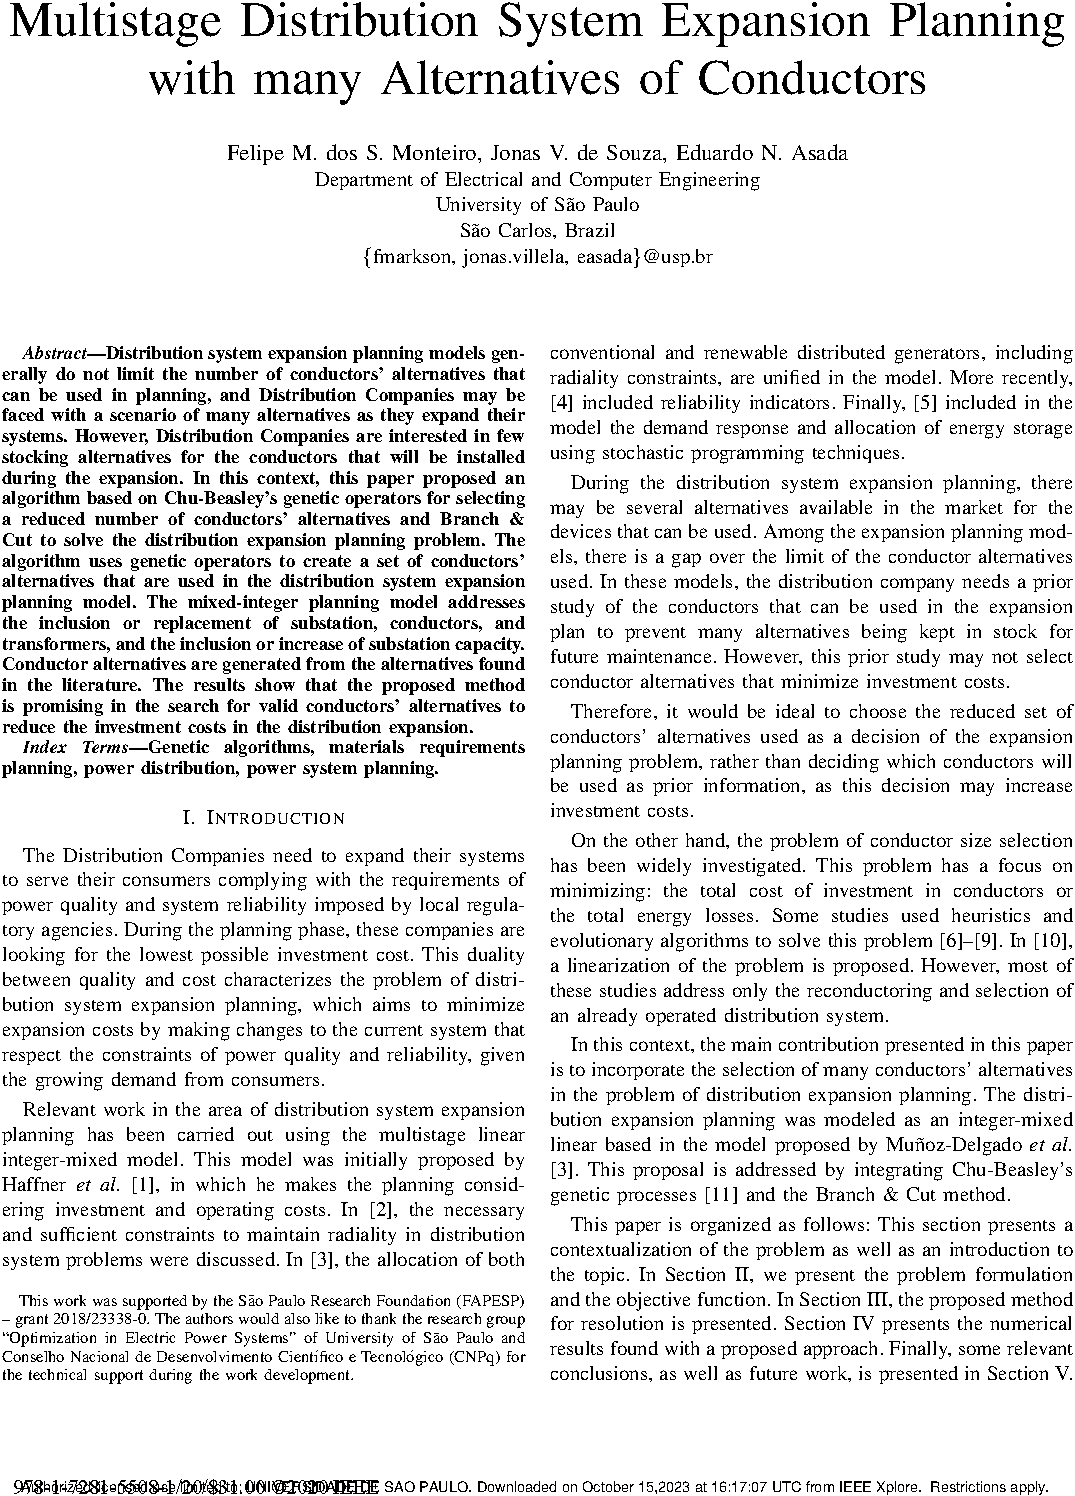
\includepdf[pages=1, scale=0.8]{Apendice/felipePaperPESD.pdf}

\chapter{Artigo sobre impactos de recursos energéticos distribuídos}
\label{sec:paperDER}
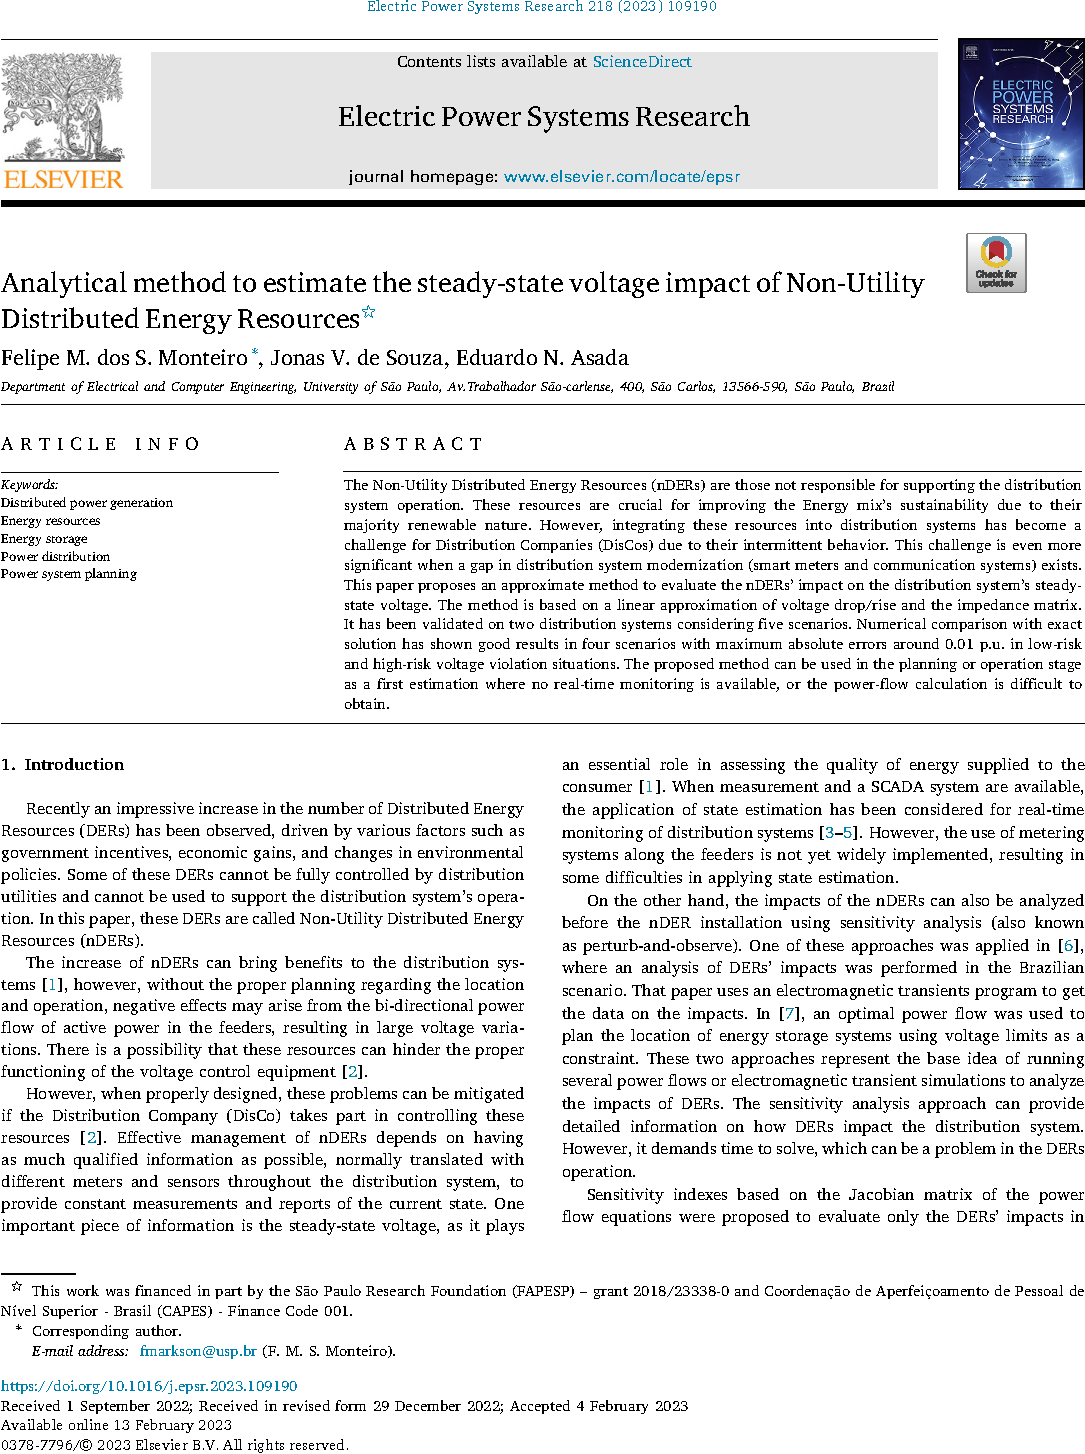
\includepdf[pages=-, scale=0.8]{Apendice/felipePaper-1.pdf}


\chapter{Tabelas com os resultados de investimentos para os sistemas utilizados}

\section{Sistema de 24 nós}
\label{sec:tab24}

\subsection{Apenas geração distribuída}
As tabelas \ref{tab:24gen1} e \ref{tab:24gen2} representam os investimentos das soluções do cenário de apenas geração distribuída no sistema de 24 nós.
\begin{table}[H]
\centering
\caption{Investimentos da solução 1 para o sistema de 24 nós para o caso de apenas geração distribuída.}
\label{tab:24gen1}
\resizebox{\textwidth}{!}{%
\begin{tabular}{cccccccccccc}
\toprule
Estágio & \multicolumn{4}{c}{Linhas} & \multicolumn{3}{c}{GDs} & \multicolumn{3}{c}{Transformadores} & Subestações \\
 & Categoria & Alternativa & Nó 1 & Nó 2 & Categoria & Alternativa & Nó & Categoria & Alternativa & Nó & Nó \\
\midrule
1 & NAF & 1 & 4 & 9 & C & 2 & 7 & 23 & NT & 1 & 24 \\
1 & NRF & 2 & 1 & 21 & C & 2 & 16 & 24 & NT & 1 & 23 \\
1 & NAF & 1 & 3 & 16 & C & 2 & 3 &  &  &  &  \\
1 & NAF & 2 & 4 & 15 & C & 2 & 15 &  &  &  &  \\
1 & NAF & 2 & 3 & 23 &  &  &  &  &  &  &  \\
1 & NAF & 2 & 17 & 22 &  &  &  &  &  &  &  \\
1 & NAF & 1 & 15 & 17 &  &  &  &  &  &  &  \\
1 & NAF & 1 & 5 & 24 &  &  &  &  &  &  &  \\
1 & NAF & 2 & 10 & 16 &  &  &  &  &  &  &  \\
1 & NAF & 2 & 7 & 23 &  &  &  &  &  &  &  \\
2 & NAF & 2 & 14 & 18 & W & 2 & 18 &  &  &  &  \\
2 & NAF & 1 & 2 & 12 & C & 2 & 13 &  &  &  &  \\
2 & NAF & 2 & 11 & 23 & C & 2 & 2 &  &  &  &  \\
2 & NAF & 1 & 6 & 13 &  &  &  &  &  &  &  \\
2 & NAF & 2 & 18 & 24 &  &  &  &  &  &  &  \\
3 & NAF & 1 & 7 & 19 & C & 2 & 17 &  &  &  &  \\
3 & NAF & 1 & 20 & 24 & W & 2 & 4 &  &  &  &  \\
3 &  &  &  &  & C & 2 & 20 &  &  &  &  \\
\bottomrule
\end{tabular}}
\\Fonte: Próprio autor
\end{table}


\begin{table}[H]
\centering
\caption{Investimentos da solução 2 para o sistema de 24 nós para o caso de apenas geração distribuída.}
\label{tab:24gen2}
\resizebox{\textwidth}{!}{%
\begin{tabular}{cccccccccccc}
\toprule
Estágio & \multicolumn{4}{c}{Linhas} & \multicolumn{3}{c}{GDs} & \multicolumn{3}{c}{Transformadores} & Subestações \\
 & Categoria & Alternativa & Nó 1 & Nó 2 & Categoria & Alternativa & Nó & Categoria & Alternativa & Nó & Nó \\
\midrule
1 & NAF & 1 & 4 & 9 & C & 2 & 7 & 23 & NT & 1 & 24 \\
1 & NRF & 2 & 1 & 21 & C & 2 & 16 & 24 & NT & 1 & 23 \\
1 & NAF & 1 & 3 & 16 & C & 2 & 3 &  &  &  &  \\
1 & NAF & 2 & 4 & 15 & C & 2 & 15 &  &  &  &  \\
1 & NAF & 2 & 3 & 23 &  &  &  &  &  &  &  \\
1 & NAF & 2 & 17 & 22 &  &  &  &  &  &  &  \\
1 & NAF & 1 & 15 & 17 &  &  &  &  &  &  &  \\
1 & NAF & 1 & 5 & 24 &  &  &  &  &  &  &  \\
1 & NAF & 2 & 10 & 16 &  &  &  &  &  &  &  \\
1 & NAF & 2 & 7 & 23 &  &  &  &  &  &  &  \\
2 & NAF & 2 & 14 & 18 & W & 2 & 18 &  &  &  &  \\
2 & NAF & 1 & 2 & 12 & C & 2 & 13 &  &  &  &  \\
2 & NAF & 2 & 11 & 23 & C & 2 & 2 &  &  &  &  \\
2 & NAF & 1 & 6 & 13 &  &  &  &  &  &  &  \\
2 & NAF & 2 & 18 & 24 &  &  &  &  &  &  &  \\
3 & NAF & 1 & 7 & 19 & C & 2 & 17 &  &  &  &  \\
3 & NAF & 1 & 20 & 24 & C & 2 & 20 &  &  &  &  \\
3 &  &  &  &  & W & 2 & 9 &  &  &  &  \\
\bottomrule
\end{tabular}}
\\Fonte: Próprio autor
\end{table}




\subsection{Apenas veículos elétricos ou cargas}
As tabelas de \ref{tab:24ev1} a \ref{tab:24ev9} representam os investimentos das soluções do cenário de apenas veículos elétricos ou cargas no sistema de 24 nós.
\begin{table}[H]
\centering
\caption{Investimentos da solução 1 para o sistema de 24 nós para o caso de apenas veículos elétricos ou cargas.}
\label{tab:24ev1}
\resizebox{\textwidth}{!}{%
\begin{tabular}{cccccccccccc}
\toprule
Estágio & \multicolumn{4}{c}{Linhas} & \multicolumn{3}{c}{GDs} & \multicolumn{3}{c}{Transformadores} & Subestações \\
 & Categoria & Alternativa & Nó 1 & Nó 2 & Categoria & Alternativa & Nó & Categoria & Alternativa & Nó & Nó \\
\midrule
1 & NAF & 1 & 4 & 9 & C & 2 & 7 & 23 & NT & 2 & 24 \\
1 & NRF & 2 & 1 & 21 & C & 2 & 16 & 24 & NT & 1 & 23 \\
1 & NAF & 1 & 3 & 16 & C & 2 & 3 &  &  &  &  \\
1 & NAF & 2 & 4 & 15 & C & 2 & 15 &  &  &  &  \\
1 & NAF & 2 & 3 & 23 &  &  &  &  &  &  &  \\
1 & NAF & 2 & 17 & 22 &  &  &  &  &  &  &  \\
1 & NAF & 1 & 5 & 24 &  &  &  &  &  &  &  \\
1 & NAF & 2 & 15 & 17 &  &  &  &  &  &  &  \\
1 & NAF & 2 & 10 & 16 &  &  &  &  &  &  &  \\
1 & NAF & 2 & 7 & 23 &  &  &  &  &  &  &  \\
2 & NAF & 2 & 14 & 18 & W & 2 & 18 & 22 &  &  &  \\
2 & NAF & 1 & 2 & 12 & C & 2 & 13 &  &  &  &  \\
2 & NAF & 2 & 11 & 23 & C & 2 & 2 &  &  &  &  \\
2 & NAF & 1 & 6 & 13 &  &  &  &  &  &  &  \\
2 & NAF & 2 & 18 & 24 &  &  &  &  &  &  &  \\
3 & NAF & 1 & 7 & 19 & C & 2 & 17 &  & NT & 1 & 22 \\
3 & NAF & 1 & 20 & 24 & C & 2 & 20 &  &  &  &  \\
3 &  &  &  &  & W & 2 & 9 &  &  &  &  \\
\bottomrule
\end{tabular}}
\\Fonte: Próprio autor
\end{table}


\begin{table}[H]
\centering
\caption{Investimentos da solução 2 para o sistema de 24 nós para o caso de apenas veículos elétricos ou cargas.}
\label{tab:24ev2}
\resizebox{\textwidth}{!}{%
\begin{tabular}{cccccccccccc}
\toprule
Estágio & \multicolumn{4}{c}{Linhas} & \multicolumn{3}{c}{GDs} & \multicolumn{3}{c}{Transformadores} & Subestações \\
 & Categoria & Alternativa & Nó 1 & Nó 2 & Categoria & Alternativa & Nó & Categoria & Alternativa & Nó & Nó \\
\midrule
1 & NRF & 2 & 1 & 21 & C & 2 & 7 & 23 & NT & 1 & 24 \\
1 & NAF & 1 & 1 & 9 & C & 2 & 16 & 24 & NT & 1 & 23 \\
1 & NAF & 2 & 11 & 23 & C & 2 & 3 & 21 &  &  &  \\
1 & NAF & 2 & 14 & 18 & C & 2 & 2 &  &  &  &  \\
1 & NAF & 1 & 5 & 24 &  &  &  &  &  &  &  \\
1 & NAF & 1 & 2 & 3 &  &  &  &  &  &  &  \\
1 & NAF & 2 & 4 & 16 &  &  &  &  &  &  &  \\
1 & NAF & 1 & 7 & 23 &  &  &  &  &  &  &  \\
1 & NAF & 1 & 10 & 16 &  &  &  &  &  &  &  \\
1 & NAF & 2 & 10 & 23 &  &  &  &  &  &  &  \\
1 & NAF & 1 & 17 & 22 &  &  &  &  &  &  &  \\
2 & NAF & 2 & 18 & 24 & C & 2 & 15 &  & NT & 1 & 21 \\
2 & NAF & 1 & 2 & 12 & W & 2 & 18 &  &  &  &  \\
2 & NAF & 1 & 15 & 17 & C & 2 & 13 &  &  &  &  \\
2 & NAF & 1 & 6 & 13 &  &  &  &  &  &  &  \\
3 & NAF & 1 & 20 & 24 & C & 2 & 17 &  &  &  &  \\
3 & NAF & 1 & 15 & 19 & C & 2 & 20 &  &  &  &  \\
3 &  &  &  &  & W & 2 & 9 &  &  &  &  \\
\bottomrule
\end{tabular}}
\\Fonte: Próprio autor
\end{table}


\begin{table}[H]
\centering
\caption{Investimentos da solução 3 para o sistema de 24 nós para o caso de apenas veículos elétricos ou cargas.}
\label{tab:24ev3}
\resizebox{\textwidth}{!}{%
\begin{tabular}{cccccccccccc}
\toprule
Estágio & \multicolumn{4}{c}{Linhas} & \multicolumn{3}{c}{GDs} & \multicolumn{3}{c}{Transformadores} & Subestações \\
 & Categoria & Alternativa & Nó 1 & Nó 2 & Categoria & Alternativa & Nó & Categoria & Alternativa & Nó & Nó \\
\midrule
1 & NRF & 2 & 1 & 21 & C & 2 & 7 & 23 & NT & 1 & 24 \\
1 & NAF & 1 & 1 & 9 & C & 2 & 16 & 24 & NT & 1 & 23 \\
1 & NAF & 1 & 5 & 24 & C & 2 & 3 &  &  &  &  \\
1 & NAF & 1 & 2 & 3 & C & 2 & 2 &  &  &  &  \\
1 & NAF & 2 & 4 & 16 &  &  &  &  &  &  &  \\
1 & NAF & 1 & 7 & 23 &  &  &  &  &  &  &  \\
1 & NAF & 1 & 10 & 16 &  &  &  &  &  &  &  \\
1 & NAF & 2 & 10 & 23 &  &  &  &  &  &  &  \\
2 & NAF & 1 & 6 & 13 & C & 2 & 15 & 21 &  &  &  \\
2 & NAF & 1 & 17 & 22 & W & 2 & 18 &  &  &  &  \\
2 & NAF & 2 & 14 & 18 & C & 2 & 13 &  &  &  &  \\
2 & NAF & 2 & 18 & 24 &  &  &  &  &  &  &  \\
2 & NAF & 1 & 2 & 12 &  &  &  &  &  &  &  \\
2 & NAF & 1 & 15 & 17 &  &  &  &  &  &  &  \\
2 & NAF & 2 & 11 & 23 &  &  &  &  &  &  &  \\
3 & NAF & 1 & 20 & 24 & C & 2 & 17 &  & NT & 1 & 21 \\
3 & NAF & 1 & 15 & 19 & C & 2 & 20 &  &  &  &  \\
3 &  &  &  &  & W & 2 & 9 &  &  &  &  \\
\bottomrule
\end{tabular}}
\\Fonte: Próprio autor
\end{table}


\begin{table}[H]
\centering
\caption{Investimentos da solução 4 para o sistema de 24 nós para o caso de apenas veículos elétricos ou cargas.}
\label{tab:24ev4}
\resizebox{\textwidth}{!}{%
\begin{tabular}{cccccccccccc}
\toprule
Estágio & \multicolumn{4}{c}{Linhas} & \multicolumn{3}{c}{GDs} & \multicolumn{3}{c}{Transformadores} & Subestações \\
 & Categoria & Alternativa & Nó 1 & Nó 2 & Categoria & Alternativa & Nó & Categoria & Alternativa & Nó & Nó \\
\midrule
1 & NAF & 1 & 4 & 9 & C & 2 & 7 & 23 & NT & 1 & 24 \\
1 & NRF & 2 & 1 & 21 & C & 2 & 16 & 24 & NT & 1 & 23 \\
1 & NAF & 1 & 3 & 16 & C & 2 & 3 &  &  &  &  \\
1 & NAF & 2 & 4 & 15 & C & 2 & 15 &  &  &  &  \\
1 & NAF & 2 & 3 & 23 &  &  &  &  &  &  &  \\
1 & NAF & 2 & 17 & 22 &  &  &  &  &  &  &  \\
1 & NAF & 1 & 5 & 24 &  &  &  &  &  &  &  \\
1 & NAF & 2 & 15 & 17 &  &  &  &  &  &  &  \\
1 & NAF & 2 & 10 & 16 &  &  &  &  &  &  &  \\
1 & NAF & 2 & 7 & 23 &  &  &  &  &  &  &  \\
2 & NAF & 2 & 14 & 18 & W & 2 & 18 & 22 &  &  &  \\
2 & NAF & 1 & 2 & 12 & C & 2 & 13 &  &  &  &  \\
2 & NAF & 2 & 11 & 23 & C & 2 & 2 &  &  &  &  \\
2 & NAF & 1 & 6 & 13 &  &  &  &  &  &  &  \\
2 & NAF & 2 & 18 & 24 &  &  &  &  &  &  &  \\
3 & NAF & 1 & 7 & 19 & C & 2 & 17 &  & NT & 1 & 22 \\
3 & NAF & 1 & 20 & 24 & C & 2 & 20 &  &  &  &  \\
3 &  &  &  &  & W & 2 & 9 &  &  &  &  \\
\bottomrule
\end{tabular}}
\\Fonte: Próprio autor
\end{table}


\begin{table}[H]
\centering
\caption{Investimentos da solução 5 para o sistema de 24 nós para o caso de apenas veículos elétricos ou cargas.}
\label{tab:24ev5}
\resizebox{\textwidth}{!}{%
\begin{tabular}{cccccccccccc}
\toprule
Estágio & \multicolumn{4}{c}{Linhas} & \multicolumn{3}{c}{GDs} & \multicolumn{3}{c}{Transformadores} & Subestações \\
 & Categoria & Alternativa & Nó 1 & Nó 2 & Categoria & Alternativa & Nó & Categoria & Alternativa & Nó & Nó \\
\midrule
1 & NAF & 1 & 4 & 9 & C & 2 & 7 & 23 & NT & 2 & 24 \\
1 & NRF & 2 & 1 & 21 & C & 2 & 16 & 24 & NT & 1 & 23 \\
1 & NAF & 2 & 3 & 23 & C & 2 & 3 &  &  &  &  \\
1 & NAF & 2 & 3 & 16 & C & 2 & 2 &  &  &  &  \\
1 & NAF & 1 & 5 & 24 &  &  &  &  &  &  &  \\
1 & NAF & 2 & 4 & 16 &  &  &  &  &  &  &  \\
1 & NAF & 1 & 7 & 23 &  &  &  &  &  &  &  \\
1 & NAF & 2 & 10 & 23 &  &  &  &  &  &  &  \\
2 & NAF & 2 & 14 & 18 & C & 2 & 15 &  &  &  &  \\
2 & NAF & 2 & 18 & 24 & W & 2 & 18 &  &  &  &  \\
2 & NAF & 1 & 2 & 12 & C & 2 & 13 &  &  &  &  \\
2 & NAF & 2 & 11 & 23 &  &  &  &  &  &  &  \\
2 & NAF & 1 & 15 & 17 &  &  &  &  &  &  &  \\
2 & NAF & 1 & 17 & 22 &  &  &  &  &  &  &  \\
2 & NAF & 1 & 6 & 13 &  &  &  &  &  &  &  \\
3 & NAF & 1 & 20 & 24 & C & 2 & 17 &  &  &  &  \\
3 & NAF & 1 & 15 & 19 & C & 2 & 20 &  &  &  &  \\
3 &  &  &  &  & W & 2 & 9 &  &  &  &  \\
\bottomrule
\end{tabular}}
\\Fonte: Próprio autor
\end{table}


\begin{table}[H]
\centering
\caption{Investimentos da solução 6 para o sistema de 24 nós para o caso de apenas veículos elétricos ou cargas.}
\label{tab:24ev6}
\resizebox{\textwidth}{!}{%
\begin{tabular}{cccccccccccc}
\toprule
Estágio & \multicolumn{4}{c}{Linhas} & \multicolumn{3}{c}{GDs} & \multicolumn{3}{c}{Transformadores} & Subestações \\
 & Categoria & Alternativa & Nó 1 & Nó 2 & Categoria & Alternativa & Nó & Categoria & Alternativa & Nó & Nó \\
\midrule
1 & NAF & 1 & 4 & 9 & C & 2 & 7 & 23 & NT & 2 & 24 \\
1 & NRF & 2 & 1 & 21 & C & 2 & 16 & 24 & NT & 1 & 23 \\
1 & NAF & 1 & 3 & 16 & C & 2 & 3 &  &  &  &  \\
1 & NAF & 2 & 3 & 23 & C & 2 & 2 &  &  &  &  \\
1 & NAF & 1 & 5 & 24 &  &  &  &  &  &  &  \\
1 & NAF & 2 & 4 & 16 &  &  &  &  &  &  &  \\
1 & NAF & 1 & 7 & 23 &  &  &  &  &  &  &  \\
1 & NAF & 2 & 10 & 23 &  &  &  &  &  &  &  \\
2 & NAF & 2 & 14 & 18 & C & 2 & 15 &  &  &  &  \\
2 & NAF & 2 & 18 & 24 & W & 2 & 18 &  &  &  &  \\
2 & NAF & 1 & 2 & 12 & C & 2 & 13 &  &  &  &  \\
2 & NAF & 2 & 11 & 23 &  &  &  &  &  &  &  \\
2 & NAF & 1 & 15 & 17 &  &  &  &  &  &  &  \\
2 & NAF & 1 & 17 & 22 &  &  &  &  &  &  &  \\
2 & NAF & 1 & 6 & 13 &  &  &  &  &  &  &  \\
3 & NAF & 1 & 20 & 24 & C & 2 & 17 &  &  &  &  \\
3 & NAF & 1 & 15 & 19 & C & 2 & 20 &  &  &  &  \\
3 &  &  &  &  & W & 2 & 9 &  &  &  &  \\
\bottomrule
\end{tabular}}
\\Fonte: Próprio autor
\end{table}


\begin{table}[H]
\centering
\caption{Investimentos da solução 7 para o sistema de 24 nós para o caso de apenas veículos elétricos ou cargas.}
\label{tab:24ev7}
\resizebox{\textwidth}{!}{%
\begin{tabular}{cccccccccccc}
\toprule
Estágio & \multicolumn{4}{c}{Linhas} & \multicolumn{3}{c}{GDs} & \multicolumn{3}{c}{Transformadores} & Subestações \\
 & Categoria & Alternativa & Nó 1 & Nó 2 & Categoria & Alternativa & Nó & Categoria & Alternativa & Nó & Nó \\
\midrule
1 & NAF & 1 & 4 & 9 & C & 2 & 7 & 23 & NT & 1 & 24 \\
1 & NRF & 2 & 1 & 21 & C & 2 & 16 & 24 & NT & 1 & 23 \\
1 & NAF & 1 & 3 & 16 & C & 2 & 3 &  &  &  &  \\
1 & NAF & 2 & 15 & 19 & C & 2 & 15 &  &  &  &  \\
1 & NAF & 2 & 3 & 23 &  &  &  &  &  &  &  \\
1 & NAF & 2 & 17 & 22 &  &  &  &  &  &  &  \\
1 & NAF & 1 & 5 & 24 &  &  &  &  &  &  &  \\
1 & NAF & 2 & 15 & 17 &  &  &  &  &  &  &  \\
1 & NAF & 1 & 7 & 19 &  &  &  &  &  &  &  \\
1 & NAF & 2 & 4 & 16 &  &  &  &  &  &  &  \\
1 & NAF & 2 & 10 & 23 &  &  &  &  &  &  &  \\
2 & NAF & 2 & 14 & 18 & W & 2 & 18 &  &  &  &  \\
2 & NAF & 2 & 18 & 24 & C & 2 & 13 &  &  &  &  \\
2 & NAF & 1 & 2 & 12 & C & 2 & 2 &  &  &  &  \\
2 & NAF & 2 & 11 & 23 &  &  &  &  &  &  &  \\
2 & NAF & 1 & 6 & 13 &  &  &  &  &  &  &  \\
3 & NAF & 1 & 20 & 24 & C & 2 & 17 &  &  &  &  \\
3 &  &  &  &  & C & 2 & 20 &  &  &  &  \\
3 &  &  &  &  & W & 2 & 9 &  &  &  &  \\
\bottomrule
\end{tabular}}
\\Fonte: Próprio autor
\end{table}


\begin{table}[H]
\centering
\caption{Investimentos da solução 8 para o sistema de 24 nós para o caso de apenas veículos elétricos ou cargas.}
\label{tab:24ev8}
\resizebox{\textwidth}{!}{%
\begin{tabular}{cccccccccccc}
\toprule
Estágio & \multicolumn{4}{c}{Linhas} & \multicolumn{3}{c}{GDs} & \multicolumn{3}{c}{Transformadores} & Subestações \\
 & Categoria & Alternativa & Nó 1 & Nó 2 & Categoria & Alternativa & Nó & Categoria & Alternativa & Nó & Nó \\
\midrule
1 & NAF & 1 & 4 & 9 & C & 2 & 7 & 23 & NT & 1 & 24 \\
1 & NRF & 2 & 1 & 21 & C & 2 & 16 & 24 & NT & 1 & 23 \\
1 & NAF & 1 & 3 & 16 & C & 2 & 3 &  &  &  &  \\
1 & NAF & 2 & 4 & 15 & C & 2 & 15 &  &  &  &  \\
1 & NAF & 2 & 3 & 23 &  &  &  &  &  &  &  \\
1 & NAF & 2 & 17 & 22 &  &  &  &  &  &  &  \\
1 & NAF & 1 & 5 & 24 &  &  &  &  &  &  &  \\
1 & NAF & 2 & 15 & 17 &  &  &  &  &  &  &  \\
1 & NAF & 2 & 10 & 16 &  &  &  &  &  &  &  \\
1 & NAF & 2 & 7 & 23 &  &  &  &  &  &  &  \\
2 & NAF & 2 & 14 & 18 & W & 2 & 18 &  &  &  &  \\
2 & NAF & 1 & 2 & 12 & C & 2 & 13 &  &  &  &  \\
2 & NAF & 2 & 11 & 23 & C & 2 & 2 &  &  &  &  \\
2 & NAF & 1 & 6 & 13 &  &  &  &  &  &  &  \\
2 & NAF & 2 & 18 & 24 &  &  &  &  &  &  &  \\
3 & NAF & 1 & 7 & 19 & C & 2 & 17 &  &  &  &  \\
3 & NAF & 1 & 20 & 24 & C & 2 & 20 &  &  &  &  \\
3 &  &  &  &  & W & 2 & 9 &  &  &  &  \\
\bottomrule
\end{tabular}}
\\Fonte: Próprio autor
\end{table}


\begin{table}[H]
\centering
\caption{Investimentos da solução 9 para o sistema de 24 nós para o caso de apenas veículos elétricos ou cargas.}
\label{tab:24ev9}
\resizebox{\textwidth}{!}{%
\begin{tabular}{cccccccccccc}
\toprule
Estágio & \multicolumn{4}{c}{Linhas} & \multicolumn{3}{c}{GDs} & \multicolumn{3}{c}{Transformadores} & Subestações \\
 & Categoria & Alternativa & Nó 1 & Nó 2 & Categoria & Alternativa & Nó & Categoria & Alternativa & Nó & Nó \\
\midrule
1 & NAF & 1 & 4 & 9 & C & 2 & 7 & 23 & NT & 1 & 24 \\
1 & NRF & 2 & 1 & 21 & C & 2 & 16 & 24 & NT & 1 & 23 \\
1 & NAF & 1 & 3 & 16 & C & 2 & 3 &  &  &  &  \\
1 & NAF & 2 & 4 & 15 & C & 2 & 15 &  &  &  &  \\
1 & NAF & 2 & 3 & 23 &  &  &  &  &  &  &  \\
1 & NAF & 2 & 17 & 22 &  &  &  &  &  &  &  \\
1 & NAF & 1 & 15 & 17 &  &  &  &  &  &  &  \\
1 & NAF & 1 & 5 & 24 &  &  &  &  &  &  &  \\
1 & NAF & 2 & 10 & 16 &  &  &  &  &  &  &  \\
1 & NAF & 2 & 7 & 23 &  &  &  &  &  &  &  \\
2 & NAF & 2 & 14 & 18 & W & 2 & 18 &  &  &  &  \\
2 & NAF & 1 & 2 & 12 & C & 2 & 13 &  &  &  &  \\
2 & NAF & 2 & 11 & 23 & C & 2 & 2 &  &  &  &  \\
2 & NAF & 1 & 6 & 13 &  &  &  &  &  &  &  \\
2 & NAF & 2 & 18 & 24 &  &  &  &  &  &  &  \\
3 & NAF & 1 & 7 & 19 & C & 2 & 17 &  &  &  &  \\
3 & NAF & 1 & 20 & 24 & C & 2 & 20 &  &  &  &  \\
3 &  &  &  &  & W & 2 & 9 &  &  &  &  \\
\bottomrule
\end{tabular}}
\\Fonte: Próprio autor
\end{table}




\subsection{Ambos}
As tabelas de \ref{tab:24both1} a \ref{tab:24both9} representam os investimentos das soluções do cenário de ambos no sistema de 24 nós.
\begin{table}[H]
\centering
\caption{Investimentos da solução 1 para o sistema de 24 nós para o caso de ambos.}
\label{tab:24both1}
\resizebox{\textwidth}{!}{%
\begin{tabular}{cccccccccccc}
\toprule
Estágio & \multicolumn{4}{c}{Linhas} & \multicolumn{3}{c}{GDs} & \multicolumn{3}{c}{Transformadores} & Subestações \\
 & Categoria & Alternativa & Nó 1 & Nó 2 & Categoria & Alternativa & Nó & Categoria & Alternativa & Nó & Nó \\
\midrule
1 & NAF & 1 & 4 & 9 & C & 2 & 7 & 23 & NT & 2 & 24 \\
1 & NRF & 2 & 1 & 21 & C & 2 & 16 & 24 & NT & 1 & 23 \\
1 & NAF & 1 & 3 & 16 & C & 2 & 3 &  &  &  &  \\
1 & NAF & 2 & 4 & 15 & C & 2 & 15 &  &  &  &  \\
1 & NAF & 2 & 3 & 23 &  &  &  &  &  &  &  \\
1 & NAF & 2 & 17 & 22 &  &  &  &  &  &  &  \\
1 & NAF & 1 & 5 & 24 &  &  &  &  &  &  &  \\
1 & NAF & 2 & 15 & 17 &  &  &  &  &  &  &  \\
1 & NAF & 2 & 10 & 16 &  &  &  &  &  &  &  \\
1 & NAF & 2 & 7 & 23 &  &  &  &  &  &  &  \\
2 & NAF & 2 & 14 & 18 & W & 2 & 18 & 22 &  &  &  \\
2 & NAF & 1 & 2 & 12 & C & 2 & 13 &  &  &  &  \\
2 & NAF & 2 & 11 & 23 & C & 2 & 2 &  &  &  &  \\
2 & NAF & 1 & 6 & 13 &  &  &  &  &  &  &  \\
2 & NAF & 2 & 18 & 24 &  &  &  &  &  &  &  \\
3 & NAF & 1 & 7 & 19 & C & 2 & 17 &  & NT & 1 & 22 \\
3 & NAF & 1 & 20 & 24 & W & 2 & 4 &  &  &  &  \\
3 &  &  &  &  & C & 2 & 20 &  &  &  &  \\
\bottomrule
\end{tabular}}
\\Fonte: Próprio autor
\end{table}


\begin{table}[H]
\centering
\caption{Investimentos da solução 2 para o sistema de 24 nós para o caso de ambos.}
\label{tab:24both2}
\resizebox{\textwidth}{!}{%
\begin{tabular}{cccccccccccc}
\toprule
Estágio & \multicolumn{4}{c}{Linhas} & \multicolumn{3}{c}{GDs} & \multicolumn{3}{c}{Transformadores} & Subestações \\
 & Categoria & Alternativa & Nó 1 & Nó 2 & Categoria & Alternativa & Nó & Categoria & Alternativa & Nó & Nó \\
\midrule
1 & NAF & 1 & 4 & 9 & C & 2 & 7 & 23 & NT & 1 & 24 \\
1 & NRF & 2 & 1 & 21 & C & 2 & 16 & 24 & NT & 1 & 23 \\
1 & NAF & 1 & 3 & 16 & C & 2 & 3 &  &  &  &  \\
1 & NAF & 2 & 4 & 15 & C & 2 & 15 &  &  &  &  \\
1 & NAF & 2 & 3 & 23 &  &  &  &  &  &  &  \\
1 & NAF & 2 & 17 & 22 &  &  &  &  &  &  &  \\
1 & NAF & 1 & 5 & 24 &  &  &  &  &  &  &  \\
1 & NAF & 2 & 15 & 17 &  &  &  &  &  &  &  \\
1 & NAF & 2 & 10 & 16 &  &  &  &  &  &  &  \\
1 & NAF & 2 & 7 & 23 &  &  &  &  &  &  &  \\
2 & NAF & 2 & 14 & 18 & W & 2 & 18 & 22 &  &  &  \\
2 & NAF & 1 & 2 & 12 & C & 2 & 13 &  &  &  &  \\
2 & NAF & 2 & 11 & 23 & C & 2 & 2 &  &  &  &  \\
2 & NAF & 1 & 6 & 13 &  &  &  &  &  &  &  \\
2 & NAF & 2 & 18 & 24 &  &  &  &  &  &  &  \\
3 & NAF & 1 & 7 & 19 & C & 2 & 17 &  & NT & 1 & 22 \\
3 & NAF & 1 & 20 & 24 & W & 2 & 4 &  &  &  &  \\
3 &  &  &  &  & C & 2 & 20 &  &  &  &  \\
\bottomrule
\end{tabular}}
\\Fonte: Próprio autor
\end{table}


\begin{table}[H]
\centering
\caption{Investimentos da solução 3 para o sistema de 24 nós para o caso de ambos.}
\label{tab:24both3}
\resizebox{\textwidth}{!}{%
\begin{tabular}{cccccccccccc}
\toprule
Estágio & \multicolumn{4}{c}{Linhas} & \multicolumn{3}{c}{GDs} & \multicolumn{3}{c}{Transformadores} & Subestações \\
 & Categoria & Alternativa & Nó 1 & Nó 2 & Categoria & Alternativa & Nó & Categoria & Alternativa & Nó & Nó \\
\midrule
1 & NAF & 1 & 4 & 9 & C & 2 & 7 & 23 & NT & 2 & 24 \\
1 & NRF & 2 & 1 & 21 & C & 2 & 16 & 24 & NT & 1 & 23 \\
1 & NAF & 2 & 3 & 23 & C & 2 & 3 &  &  &  &  \\
1 & NAF & 2 & 3 & 16 & C & 2 & 2 &  &  &  &  \\
1 & NAF & 1 & 5 & 24 &  &  &  &  &  &  &  \\
1 & NAF & 2 & 4 & 16 &  &  &  &  &  &  &  \\
1 & NAF & 1 & 7 & 23 &  &  &  &  &  &  &  \\
1 & NAF & 2 & 10 & 23 &  &  &  &  &  &  &  \\
2 & NAF & 2 & 14 & 18 & C & 2 & 15 &  &  &  &  \\
2 & NAF & 2 & 18 & 24 & W & 2 & 18 &  &  &  &  \\
2 & NAF & 1 & 20 & 24 & C & 2 & 13 &  &  &  &  \\
2 & NAF & 1 & 2 & 12 &  &  &  &  &  &  &  \\
2 & NAF & 2 & 11 & 23 &  &  &  &  &  &  &  \\
2 & NAF & 1 & 15 & 17 &  &  &  &  &  &  &  \\
2 & NAF & 1 & 17 & 22 &  &  &  &  &  &  &  \\
2 & NAF & 1 & 6 & 13 &  &  &  &  &  &  &  \\
3 & NAF & 1 & 15 & 19 & C & 2 & 17 &  &  &  &  \\
3 &  &  &  &  & W & 2 & 4 &  &  &  &  \\
3 &  &  &  &  & C & 2 & 20 &  &  &  &  \\
\bottomrule
\end{tabular}}
\\Fonte: Próprio autor
\end{table}


\begin{table}[H]
\centering
\caption{Investimentos da solução 4 para o sistema de 24 nós para o caso de ambos.}
\label{tab:24both4}
\resizebox{\textwidth}{!}{%
\begin{tabular}{cccccccccccc}
\toprule
Estágio & \multicolumn{4}{c}{Linhas} & \multicolumn{3}{c}{GDs} & \multicolumn{3}{c}{Transformadores} & Subestações \\
 & Categoria & Alternativa & Nó 1 & Nó 2 & Categoria & Alternativa & Nó & Categoria & Alternativa & Nó & Nó \\
\midrule
1 & NAF & 1 & 4 & 9 & C & 2 & 7 & 23 & NT & 2 & 24 \\
1 & NRF & 2 & 1 & 21 & C & 2 & 16 & 24 & NT & 1 & 23 \\
1 & NAF & 2 & 3 & 23 & C & 2 & 3 &  &  &  &  \\
1 & NAF & 2 & 3 & 16 & C & 2 & 2 &  &  &  &  \\
1 & NAF & 1 & 5 & 24 &  &  &  &  &  &  &  \\
1 & NAF & 2 & 4 & 16 &  &  &  &  &  &  &  \\
1 & NAF & 1 & 7 & 23 &  &  &  &  &  &  &  \\
1 & NAF & 2 & 10 & 23 &  &  &  &  &  &  &  \\
2 & NAF & 2 & 14 & 18 & C & 2 & 15 &  &  &  &  \\
2 & NAF & 2 & 18 & 24 & W & 2 & 18 &  &  &  &  \\
2 & NAF & 1 & 2 & 12 & C & 2 & 13 &  &  &  &  \\
2 & NAF & 2 & 11 & 23 &  &  &  &  &  &  &  \\
2 & NAF & 1 & 15 & 17 &  &  &  &  &  &  &  \\
2 & NAF & 1 & 17 & 22 &  &  &  &  &  &  &  \\
2 & NAF & 1 & 6 & 13 &  &  &  &  &  &  &  \\
3 & NAF & 1 & 20 & 24 & C & 2 & 17 &  &  &  &  \\
3 & NAF & 1 & 15 & 19 & W & 2 & 4 &  &  &  &  \\
3 &  &  &  &  & C & 2 & 20 &  &  &  &  \\
\bottomrule
\end{tabular}}
\\Fonte: Próprio autor
\end{table}


\begin{table}[H]
\centering
\caption{Investimentos da solução 5 para o sistema de 24 nós para o caso de ambos.}
\label{tab:24both5}
\resizebox{\textwidth}{!}{%
\begin{tabular}{cccccccccccc}
\toprule
Estágio & \multicolumn{4}{c}{Linhas} & \multicolumn{3}{c}{GDs} & \multicolumn{3}{c}{Transformadores} & Subestações \\
 & Categoria & Alternativa & Nó 1 & Nó 2 & Categoria & Alternativa & Nó & Categoria & Alternativa & Nó & Nó \\
\midrule
1 & NAF & 1 & 4 & 9 & C & 2 & 7 & 23 & NT & 2 & 24 \\
1 & NRF & 2 & 1 & 21 & C & 2 & 16 & 24 & NT & 1 & 23 \\
1 & NAF & 1 & 3 & 16 & C & 2 & 3 &  &  &  &  \\
1 & NAF & 2 & 3 & 23 & C & 2 & 2 &  &  &  &  \\
1 & NAF & 1 & 5 & 24 &  &  &  &  &  &  &  \\
1 & NAF & 2 & 4 & 16 &  &  &  &  &  &  &  \\
1 & NAF & 1 & 7 & 23 &  &  &  &  &  &  &  \\
1 & NAF & 2 & 10 & 23 &  &  &  &  &  &  &  \\
2 & NAF & 2 & 14 & 18 & C & 2 & 15 &  &  &  &  \\
2 & NAF & 2 & 18 & 24 & W & 2 & 18 &  &  &  &  \\
2 & NAF & 1 & 2 & 12 & C & 2 & 13 &  &  &  &  \\
2 & NAF & 2 & 11 & 23 &  &  &  &  &  &  &  \\
2 & NAF & 1 & 15 & 17 &  &  &  &  &  &  &  \\
2 & NAF & 1 & 17 & 22 &  &  &  &  &  &  &  \\
2 & NAF & 1 & 6 & 13 &  &  &  &  &  &  &  \\
3 & NAF & 1 & 20 & 24 & C & 2 & 17 &  &  &  &  \\
3 & NAF & 1 & 15 & 19 & W & 2 & 4 &  &  &  &  \\
3 &  &  &  &  & C & 2 & 20 &  &  &  &  \\
\bottomrule
\end{tabular}}
\\Fonte: Próprio autor
\end{table}


\begin{table}[H]
\centering
\caption{Investimentos da solução 6 para o sistema de 24 nós para o caso de ambos.}
\label{tab:24both6}
\resizebox{\textwidth}{!}{%
\begin{tabular}{cccccccccccc}
\toprule
Estágio & \multicolumn{4}{c}{Linhas} & \multicolumn{3}{c}{GDs} & \multicolumn{3}{c}{Transformadores} & Subestações \\
 & Categoria & Alternativa & Nó 1 & Nó 2 & Categoria & Alternativa & Nó & Categoria & Alternativa & Nó & Nó \\
\midrule
1 & NAF & 1 & 4 & 9 & C & 2 & 7 & 23 & NT & 2 & 24 \\
1 & NRF & 2 & 1 & 21 & C & 2 & 16 & 24 & NT & 1 & 23 \\
1 & NAF & 1 & 3 & 16 & C & 2 & 3 &  &  &  &  \\
1 & NAF & 2 & 3 & 23 & C & 2 & 2 &  &  &  &  \\
1 & NAF & 1 & 5 & 24 &  &  &  &  &  &  &  \\
1 & NAF & 2 & 4 & 16 &  &  &  &  &  &  &  \\
1 & NAF & 1 & 7 & 23 &  &  &  &  &  &  &  \\
1 & NAF & 2 & 10 & 23 &  &  &  &  &  &  &  \\
2 & NAF & 2 & 14 & 18 & C & 2 & 15 &  &  &  &  \\
2 & NAF & 2 & 18 & 24 & W & 2 & 18 &  &  &  &  \\
2 & NAF & 1 & 2 & 12 & C & 2 & 13 &  &  &  &  \\
2 & NAF & 2 & 11 & 23 &  &  &  &  &  &  &  \\
2 & NAF & 1 & 15 & 17 &  &  &  &  &  &  &  \\
2 & NAF & 1 & 17 & 22 &  &  &  &  &  &  &  \\
2 & NAF & 1 & 6 & 13 &  &  &  &  &  &  &  \\
3 & NAF & 1 & 20 & 24 & C & 2 & 17 &  &  &  &  \\
3 & NAF & 1 & 15 & 19 & C & 2 & 20 &  &  &  &  \\
3 &  &  &  &  & W & 2 & 9 &  &  &  &  \\
\bottomrule
\end{tabular}}
\\Fonte: Próprio autor
\end{table}


\begin{table}[H]
\centering
\caption{Investimentos da solução 7 para o sistema de 24 nós para o caso de ambos.}
\label{tab:24both7}
\resizebox{\textwidth}{!}{%
\begin{tabular}{cccccccccccc}
\toprule
Estágio & \multicolumn{4}{c}{Linhas} & \multicolumn{3}{c}{GDs} & \multicolumn{3}{c}{Transformadores} & Subestações \\
 & Categoria & Alternativa & Nó 1 & Nó 2 & Categoria & Alternativa & Nó & Categoria & Alternativa & Nó & Nó \\
\midrule
1 & NAF & 1 & 4 & 9 & C & 2 & 7 & 23 & NT & 1 & 24 \\
1 & NRF & 2 & 1 & 21 & C & 2 & 16 & 24 & NT & 1 & 23 \\
1 & NAF & 1 & 3 & 16 & C & 2 & 3 &  &  &  &  \\
1 & NAF & 2 & 15 & 19 & C & 2 & 15 &  &  &  &  \\
1 & NAF & 2 & 3 & 23 &  &  &  &  &  &  &  \\
1 & NAF & 2 & 17 & 22 &  &  &  &  &  &  &  \\
1 & NAF & 1 & 5 & 24 &  &  &  &  &  &  &  \\
1 & NAF & 2 & 15 & 17 &  &  &  &  &  &  &  \\
1 & NAF & 1 & 7 & 19 &  &  &  &  &  &  &  \\
1 & NAF & 2 & 4 & 16 &  &  &  &  &  &  &  \\
1 & NAF & 2 & 10 & 23 &  &  &  &  &  &  &  \\
2 & NAF & 2 & 14 & 18 & W & 2 & 18 &  &  &  &  \\
2 & NAF & 2 & 18 & 24 & C & 2 & 13 &  &  &  &  \\
2 & NAF & 1 & 2 & 12 & C & 2 & 2 &  &  &  &  \\
2 & NAF & 2 & 11 & 23 &  &  &  &  &  &  &  \\
2 & NAF & 1 & 6 & 13 &  &  &  &  &  &  &  \\
3 & NAF & 1 & 20 & 24 & C & 2 & 17 &  &  &  &  \\
3 &  &  &  &  & C & 2 & 20 &  &  &  &  \\
3 &  &  &  &  & W & 2 & 9 &  &  &  &  \\
\bottomrule
\end{tabular}}
\\Fonte: Próprio autor
\end{table}


\begin{table}[H]
\centering
\caption{Investimentos da solução 8 para o sistema de 24 nós para o caso de ambos.}
\label{tab:24both8}
\resizebox{\textwidth}{!}{%
\begin{tabular}{cccccccccccc}
\toprule
Estágio & \multicolumn{4}{c}{Linhas} & \multicolumn{3}{c}{GDs} & \multicolumn{3}{c}{Transformadores} & Subestações \\
 & Categoria & Alternativa & Nó 1 & Nó 2 & Categoria & Alternativa & Nó & Categoria & Alternativa & Nó & Nó \\
\midrule
1 & NAF & 1 & 4 & 9 & C & 2 & 7 & 23 & NT & 1 & 24 \\
1 & NRF & 2 & 1 & 21 & C & 2 & 16 & 24 & NT & 1 & 23 \\
1 & NAF & 1 & 3 & 16 & C & 2 & 3 &  &  &  &  \\
1 & NAF & 2 & 4 & 15 & C & 2 & 15 &  &  &  &  \\
1 & NAF & 2 & 3 & 23 &  &  &  &  &  &  &  \\
1 & NAF & 2 & 17 & 22 &  &  &  &  &  &  &  \\
1 & NAF & 1 & 5 & 24 &  &  &  &  &  &  &  \\
1 & NAF & 2 & 15 & 17 &  &  &  &  &  &  &  \\
1 & NAF & 2 & 10 & 16 &  &  &  &  &  &  &  \\
1 & NAF & 2 & 7 & 23 &  &  &  &  &  &  &  \\
2 & NAF & 2 & 14 & 18 & W & 2 & 18 &  &  &  &  \\
2 & NAF & 1 & 2 & 12 & C & 2 & 13 &  &  &  &  \\
2 & NAF & 2 & 11 & 23 & C & 2 & 2 &  &  &  &  \\
2 & NAF & 1 & 6 & 13 &  &  &  &  &  &  &  \\
2 & NAF & 2 & 18 & 24 &  &  &  &  &  &  &  \\
3 & NAF & 1 & 7 & 19 & C & 2 & 17 &  &  &  &  \\
3 & NAF & 1 & 20 & 24 & C & 2 & 20 &  &  &  &  \\
3 &  &  &  &  & W & 2 & 9 &  &  &  &  \\
\bottomrule
\end{tabular}}
\\Fonte: Próprio autor
\end{table}


\begin{table}[H]
\centering
\caption{Investimentos da solução 9 para o sistema de 24 nós para o caso de ambos.}
\label{tab:24both9}
\resizebox{\textwidth}{!}{%
\begin{tabular}{cccccccccccc}
\toprule
Estágio & \multicolumn{4}{c}{Linhas} & \multicolumn{3}{c}{GDs} & \multicolumn{3}{c}{Transformadores} & Subestações \\
 & Categoria & Alternativa & Nó 1 & Nó 2 & Categoria & Alternativa & Nó & Categoria & Alternativa & Nó & Nó \\
\midrule
1 & NAF & 1 & 4 & 9 & C & 2 & 7 & 23 & NT & 1 & 24 \\
1 & NRF & 2 & 1 & 21 & C & 2 & 16 & 24 & NT & 1 & 23 \\
1 & NAF & 1 & 3 & 16 & C & 2 & 3 &  &  &  &  \\
1 & NAF & 2 & 4 & 15 & C & 2 & 15 &  &  &  &  \\
1 & NAF & 2 & 3 & 23 &  &  &  &  &  &  &  \\
1 & NAF & 2 & 17 & 22 &  &  &  &  &  &  &  \\
1 & NAF & 1 & 15 & 17 &  &  &  &  &  &  &  \\
1 & NAF & 1 & 5 & 24 &  &  &  &  &  &  &  \\
1 & NAF & 2 & 10 & 16 &  &  &  &  &  &  &  \\
1 & NAF & 2 & 7 & 23 &  &  &  &  &  &  &  \\
2 & NAF & 2 & 14 & 18 & W & 2 & 18 &  &  &  &  \\
2 & NAF & 1 & 2 & 12 & C & 2 & 13 &  &  &  &  \\
2 & NAF & 2 & 11 & 23 & C & 2 & 2 &  &  &  &  \\
2 & NAF & 1 & 6 & 13 &  &  &  &  &  &  &  \\
2 & NAF & 2 & 18 & 24 &  &  &  &  &  &  &  \\
3 & NAF & 1 & 7 & 19 & C & 2 & 17 &  &  &  &  \\
3 & NAF & 1 & 20 & 24 & C & 2 & 20 &  &  &  &  \\
3 &  &  &  &  & W & 2 & 9 &  &  &  &  \\
\bottomrule
\end{tabular}}
\\Fonte: Próprio autor
\end{table}




\newpage
\section{Sistema de 54 nós}
\label{sec:tab54}

\subsection{Apenas geração distribuída}
As tabelas \ref{tab:54gen1} representa os investimentos da solução do cenário de apenas geração distribuída no sistema de 54 nós.
\begin{table}[H]
\centering
\caption{Investimentos da solução 1 para o sistema de 54 nós para o caso de apenas geração distribuída.}
\label{tab:54gen1}
\resizebox{\textwidth}{!}{%
\begin{tabular}{ccccccccccc}
\toprule
\multicolumn{4}{c}{Linhas} & \multicolumn{3}{c}{GDs} & \multicolumn{3}{c}{Transformadores} & Subestações \\
Categoria & Alternativa & Nó 1 & Nó 2 & Categoria & Alternativa & Nó & Categoria & Alternativa & Nó & Nó \\
\midrule
NAF & 1 & 44 & 45 & C & 2 & 23 & NT & 2 & 53 & 53 \\
NAF & 2 & 27 & 28 & W & 2 & 3 & NT & 2 & 51 & 51 \\
NAF & 1 & 26 & 27 & C & 2 & 43 & NT & 2 & 54 & 54 \\
NAF & 2 & 35 & 36 & C & 2 & 12 &  &  &  &  \\
NAF & 2 & 18 & 19 & C & 2 & 42 &  &  &  &  \\
NAF & 1 & 42 & 48 & C & 2 & 24 &  &  &  &  \\
NRF & 2 & 14 & 52 & C & 2 & 4 &  &  &  &  \\
NAF & 1 & 32 & 39 & C & 2 & 3 &  &  &  &  \\
NAF & 1 & 42 & 47 & W & 2 & 23 &  &  &  &  \\
NAF & 1 & 36 & 53 & C & 2 & 15 &  &  &  &  \\
NAF & 1 & 10 & 31 & W & 2 & 42 &  &  &  &  \\
NAF & 1 & 34 & 35 & PV & 2 & 12 &  &  &  &  \\
NAF & 1 & 8 & 33 & W & 2 & 15 &  &  &  &  \\
NRF & 2 & 11 & 52 & PV & 2 & 24 &  &  &  &  \\
NAF & 1 & 30 & 43 & C & 2 & 36 &  &  &  &  \\
NAF & 1 & 17 & 18 & PV & 2 & 36 &  &  &  &  \\
NAF & 1 & 38 & 44 & W & 2 & 35 &  &  &  &  \\
NAF & 1 & 22 & 23 & PV & 2 & 4 &  &  &  &  \\
NAF & 2 & 28 & 53 & PV & 2 & 43 &  &  &  &  \\
NAF & 1 & 23 & 24 &  &  &  &  &  &  &  \\
NAF & 2 & 37 & 43 &  &  &  &  &  &  &  \\
NAF & 1 & 29 & 30 &  &  &  &  &  &  &  \\
NAF & 2 & 21 & 54 &  &  &  &  &  &  &  \\
NRF & 1 & 3 & 4 &  &  &  &  &  &  &  \\
NRF & 1 & 1 & 9 &  &  &  &  &  &  &  \\
NRF & 1 & 3 & 51 &  &  &  &  &  &  &  \\
NAF & 2 & 41 & 53 &  &  &  &  &  &  &  \\
NAF & 1 & 46 & 47 &  &  &  &  &  &  &  \\
NAF & 1 & 14 & 50 &  &  &  &  &  &  &  \\
NRF & 2 & 1 & 51 &  &  &  &  &  &  &  \\
NAF & 2 & 31 & 37 &  &  &  &  &  &  &  \\
NAF & 2 & 30 & 54 &  &  &  &  &  &  &  \\
NAF & 1 & 24 & 25 &  &  &  &  &  &  &  \\
NAF & 1 & 40 & 41 &  &  &  &  &  &  &  \\
NAF & 2 & 12 & 45 &  &  &  &  &  &  &  \\
NAF & 1 & 19 & 20 &  &  &  &  &  &  &  \\
NAF & 1 & 48 & 49 &  &  &  &  &  &  &  \\
NAF & 2 & 41 & 42 &  &  &  &  &  &  &  \\
NAF & 1 & 9 & 23 &  &  &  &  &  &  &  \\
NAF & 2 & 18 & 21 &  &  &  &  &  &  &  \\
NAF & 1 & 33 & 39 &  &  &  &  &  &  &  \\
\bottomrule
\end{tabular}}
\\Fonte: Próprio autor
\end{table}




\subsection{Apenas veículos elétricos ou cargas}
As tabelas de \ref{tab:54ev1} a \ref{tab:54ev4} representam os investimentos das soluções do cenário de apenas veículos elétricos ou cargas no sistema de 54 nós.
\begin{table}[H]
\centering
\caption{Investimentos da solução 1 para o sistema de 54 nós para o caso de apenas veículos elétricos ou cargas.}
\label{tab:54ev1}
\resizebox{\textwidth}{!}{%
\begin{tabular}{ccccccccccc}
\toprule
\multicolumn{4}{c}{Linhas} & \multicolumn{3}{c}{GDs} & \multicolumn{3}{c}{Transformadores} & Subestações \\
Categoria & Alternativa & Nó 1 & Nó 2 & Categoria & Alternativa & Nó & Categoria & Alternativa & Nó & Nó \\
\midrule
NAF & 1 & 44 & 45 & C & 2 & 23 & NT & 2 & 52 & 53 \\
NAF & 2 & 27 & 28 & W & 2 & 3 & NT & 2 & 53 & 51 \\
NAF & 1 & 26 & 27 & C & 2 & 43 & NT & 2 & 51 & 54 \\
NAF & 2 & 35 & 36 & C & 2 & 12 & NT & 2 & 54 & 52 \\
NAF & 1 & 14 & 46 & C & 2 & 42 &  &  &  &  \\
NAF & 2 & 18 & 19 & C & 2 & 24 &  &  &  &  \\
NAF & 2 & 30 & 43 & C & 2 & 4 &  &  &  &  \\
NAF & 1 & 42 & 48 & C & 2 & 3 &  &  &  &  \\
NRF & 2 & 14 & 52 & W & 2 & 23 &  &  &  &  \\
NAF & 1 & 32 & 39 & C & 2 & 15 &  &  &  &  \\
NAF & 1 & 42 & 47 & W & 2 & 42 &  &  &  &  \\
NAF & 1 & 36 & 53 & PV & 2 & 12 &  &  &  &  \\
NAF & 1 & 34 & 35 & W & 2 & 15 &  &  &  &  \\
NAF & 1 & 8 & 33 & PV & 2 & 24 &  &  &  &  \\
NRF & 2 & 11 & 52 & C & 2 & 36 &  &  &  &  \\
NAF & 2 & 10 & 23 & PV & 2 & 36 &  &  &  &  \\
NAF & 1 & 38 & 44 & W & 2 & 35 &  &  &  &  \\
NAF & 1 & 9 & 17 & PV & 2 & 4 &  &  &  &  \\
NAF & 1 & 9 & 22 & PV & 2 & 43 &  &  &  &  \\
NAF & 2 & 28 & 53 &  &  &  &  &  &  &  \\
NAF & 2 & 37 & 43 &  &  &  &  &  &  &  \\
NAF & 1 & 29 & 30 &  &  &  &  &  &  &  \\
NAF & 1 & 41 & 42 &  &  &  &  &  &  &  \\
NAF & 2 & 21 & 54 &  &  &  &  &  &  &  \\
NRF & 1 & 3 & 4 &  &  &  &  &  &  &  \\
NRF & 1 & 3 & 51 &  &  &  &  &  &  &  \\
NAF & 2 & 41 & 53 &  &  &  &  &  &  &  \\
NAF & 2 & 23 & 24 &  &  &  &  &  &  &  \\
NAF & 1 & 14 & 50 &  &  &  &  &  &  &  \\
NAF & 2 & 24 & 25 &  &  &  &  &  &  &  \\
NRF & 2 & 1 & 51 &  &  &  &  &  &  &  \\
NAF & 2 & 31 & 37 &  &  &  &  &  &  &  \\
NAF & 2 & 30 & 54 &  &  &  &  &  &  &  \\
NAF & 1 & 40 & 41 &  &  &  &  &  &  &  \\
NAF & 2 & 12 & 45 &  &  &  &  &  &  &  \\
NAF & 1 & 19 & 20 &  &  &  &  &  &  &  \\
NAF & 2 & 10 & 31 &  &  &  &  &  &  &  \\
NAF & 1 & 48 & 49 &  &  &  &  &  &  &  \\
NRF & 2 & 1 & 9 &  &  &  &  &  &  &  \\
NAF & 2 & 18 & 21 &  &  &  &  &  &  &  \\
NAF & 1 & 33 & 39 &  &  &  &  &  &  &  \\
\bottomrule
\end{tabular}}
\\Fonte: Próprio autor
\end{table}


\begin{table}[H]
\centering
\caption{Investimentos da solução 2 para o sistema de 54 nós para o caso de apenas veículos elétricos ou cargas.}
\label{tab:54ev2}
\resizebox{\textwidth}{!}{%
\begin{tabular}{ccccccccccc}
\toprule
\multicolumn{4}{c}{Linhas} & \multicolumn{3}{c}{GDs} & \multicolumn{3}{c}{Transformadores} & Subestações \\
Categoria & Alternativa & Nó 1 & Nó 2 & Categoria & Alternativa & Nó & Categoria & Alternativa & Nó & Nó \\
\midrule
NAF & 1 & 44 & 45 & C & 2 & 23 & NT & 2 & 52 & 53 \\
NAF & 2 & 27 & 28 & W & 2 & 3 & NT & 2 & 53 & 51 \\
NRF & 1 & 11 & 12 & C & 2 & 43 & NT & 2 & 51 & 54 \\
NAF & 1 & 26 & 27 & C & 2 & 12 & NT & 2 & 54 & 52 \\
NAF & 2 & 35 & 36 & C & 2 & 42 &  &  &  &  \\
NAF & 2 & 18 & 19 & C & 2 & 24 &  &  &  &  \\
NAF & 1 & 16 & 40 & C & 2 & 4 &  &  &  &  \\
NRF & 2 & 14 & 52 & C & 2 & 3 &  &  &  &  \\
NAF & 1 & 32 & 39 & W & 2 & 23 &  &  &  &  \\
NAF & 1 & 10 & 23 & C & 2 & 15 &  &  &  &  \\
NAF & 1 & 42 & 47 & W & 2 & 42 &  &  &  &  \\
NAF & 1 & 36 & 53 & PV & 2 & 12 &  &  &  &  \\
NAF & 1 & 34 & 35 & W & 2 & 15 &  &  &  &  \\
NAF & 1 & 8 & 33 & PV & 2 & 24 &  &  &  &  \\
NRF & 2 & 11 & 52 & C & 2 & 36 &  &  &  &  \\
NAF & 1 & 31 & 37 & PV & 2 & 36 &  &  &  &  \\
NAF & 1 & 38 & 44 & W & 2 & 35 &  &  &  &  \\
NAF & 1 & 9 & 17 & PV & 2 & 4 &  &  &  &  \\
NAF & 1 & 30 & 54 & PV & 2 & 43 &  &  &  &  \\
NAF & 1 & 22 & 23 &  &  &  &  &  &  &  \\
NAF & 2 & 28 & 53 &  &  &  &  &  &  &  \\
NAF & 1 & 23 & 24 &  &  &  &  &  &  &  \\
NAF & 1 & 13 & 43 &  &  &  &  &  &  &  \\
NAF & 2 & 37 & 43 &  &  &  &  &  &  &  \\
NAF & 1 & 29 & 30 &  &  &  &  &  &  &  \\
NAF & 2 & 21 & 54 &  &  &  &  &  &  &  \\
NRF & 1 & 3 & 4 &  &  &  &  &  &  &  \\
NRF & 1 & 1 & 9 &  &  &  &  &  &  &  \\
NRF & 1 & 3 & 51 &  &  &  &  &  &  &  \\
NAF & 2 & 41 & 53 &  &  &  &  &  &  &  \\
NAF & 1 & 46 & 47 &  &  &  &  &  &  &  \\
NAF & 2 & 22 & 54 &  &  &  &  &  &  &  \\
NRF & 2 & 1 & 51 &  &  &  &  &  &  &  \\
NAF & 1 & 24 & 25 &  &  &  &  &  &  &  \\
NAF & 2 & 42 & 48 &  &  &  &  &  &  &  \\
NAF & 2 & 12 & 45 &  &  &  &  &  &  &  \\
NAF & 1 & 19 & 20 &  &  &  &  &  &  &  \\
NRF & 1 & 14 & 15 &  &  &  &  &  &  &  \\
NAF & 1 & 48 & 49 &  &  &  &  &  &  &  \\
NAF & 1 & 49 & 50 &  &  &  &  &  &  &  \\
NAF & 2 & 41 & 42 &  &  &  &  &  &  &  \\
NAF & 2 & 18 & 21 &  &  &  &  &  &  &  \\
NAF & 1 & 33 & 39 &  &  &  &  &  &  &  \\
\bottomrule
\end{tabular}}
\\Fonte: Próprio autor
\end{table}


\begin{table}[H]
\centering
\caption{Investimentos da solução 3 para o sistema de 54 nós para o caso de apenas veículos elétricos ou cargas.}
\label{tab:54ev3}
\resizebox{\textwidth}{!}{%
\begin{tabular}{ccccccccccc}
\toprule
\multicolumn{4}{c}{Linhas} & \multicolumn{3}{c}{GDs} & \multicolumn{3}{c}{Transformadores} & Subestações \\
Categoria & Alternativa & Nó 1 & Nó 2 & Categoria & Alternativa & Nó & Categoria & Alternativa & Nó & Nó \\
\midrule
NAF & 1 & 44 & 45 & C & 2 & 23 & NT & 2 & 52 & 53 \\
NAF & 2 & 27 & 28 & W & 2 & 3 & NT & 2 & 53 & 51 \\
NAF & 1 & 26 & 27 & C & 2 & 43 & NT & 2 & 51 & 54 \\
NAF & 2 & 35 & 36 & C & 2 & 12 & NT & 2 & 54 & 52 \\
NAF & 1 & 14 & 46 & C & 2 & 42 &  &  &  &  \\
NAF & 2 & 18 & 19 & C & 2 & 24 &  &  &  &  \\
NAF & 1 & 42 & 48 & C & 2 & 4 &  &  &  &  \\
NRF & 2 & 14 & 52 & C & 2 & 3 &  &  &  &  \\
NAF & 1 & 32 & 39 & W & 2 & 23 &  &  &  &  \\
NAF & 1 & 42 & 47 & C & 2 & 15 &  &  &  &  \\
NAF & 1 & 36 & 53 & W & 2 & 42 &  &  &  &  \\
NAF & 1 & 10 & 31 & PV & 2 & 12 &  &  &  &  \\
NAF & 1 & 34 & 35 & W & 2 & 15 &  &  &  &  \\
NAF & 1 & 8 & 33 & PV & 2 & 24 &  &  &  &  \\
NRF & 2 & 11 & 52 & C & 2 & 36 &  &  &  &  \\
NAF & 1 & 30 & 43 & PV & 2 & 36 &  &  &  &  \\
NAF & 1 & 17 & 18 & W & 2 & 35 &  &  &  &  \\
NAF & 1 & 38 & 44 & PV & 2 & 4 &  &  &  &  \\
NAF & 1 & 22 & 23 & PV & 2 & 43 &  &  &  &  \\
NAF & 2 & 28 & 53 &  &  &  &  &  &  &  \\
NAF & 1 & 23 & 24 &  &  &  &  &  &  &  \\
NAF & 2 & 37 & 43 &  &  &  &  &  &  &  \\
NAF & 1 & 29 & 30 &  &  &  &  &  &  &  \\
NAF & 1 & 41 & 42 &  &  &  &  &  &  &  \\
NAF & 2 & 21 & 54 &  &  &  &  &  &  &  \\
NRF & 1 & 3 & 4 &  &  &  &  &  &  &  \\
NRF & 1 & 1 & 9 &  &  &  &  &  &  &  \\
NRF & 1 & 3 & 51 &  &  &  &  &  &  &  \\
NAF & 2 & 41 & 53 &  &  &  &  &  &  &  \\
NAF & 1 & 14 & 50 &  &  &  &  &  &  &  \\
NRF & 2 & 1 & 51 &  &  &  &  &  &  &  \\
NAF & 2 & 31 & 37 &  &  &  &  &  &  &  \\
NAF & 2 & 30 & 54 &  &  &  &  &  &  &  \\
NAF & 1 & 24 & 25 &  &  &  &  &  &  &  \\
NAF & 1 & 40 & 41 &  &  &  &  &  &  &  \\
NAF & 2 & 12 & 45 &  &  &  &  &  &  &  \\
NAF & 1 & 19 & 20 &  &  &  &  &  &  &  \\
NAF & 1 & 48 & 49 &  &  &  &  &  &  &  \\
NAF & 1 & 9 & 23 &  &  &  &  &  &  &  \\
NAF & 2 & 18 & 21 &  &  &  &  &  &  &  \\
NAF & 1 & 33 & 39 &  &  &  &  &  &  &  \\
\bottomrule
\end{tabular}}
\\Fonte: Próprio autor
\end{table}


\begin{table}[H]
\centering
\caption{Investimentos da solução 4 para o sistema de 54 nós para o caso de apenas veículos elétricos ou cargas.}
\label{tab:54ev4}
\resizebox{\textwidth}{!}{%
\begin{tabular}{ccccccccccc}
\toprule
\multicolumn{4}{c}{Linhas} & \multicolumn{3}{c}{GDs} & \multicolumn{3}{c}{Transformadores} & Subestações \\
Categoria & Alternativa & Nó 1 & Nó 2 & Categoria & Alternativa & Nó & Categoria & Alternativa & Nó & Nó \\
\midrule
NAF & 1 & 44 & 45 & C & 2 & 23 & NT & 2 & 53 & 53 \\
NAF & 2 & 27 & 28 & W & 2 & 3 & NT & 2 & 51 & 51 \\
NAF & 1 & 26 & 27 & C & 2 & 43 & NT & 2 & 54 & 54 \\
NAF & 2 & 35 & 36 & C & 2 & 12 &  &  &  &  \\
NAF & 2 & 18 & 19 & C & 2 & 42 &  &  &  &  \\
NAF & 1 & 42 & 48 & C & 2 & 24 &  &  &  &  \\
NRF & 2 & 14 & 52 & C & 2 & 4 &  &  &  &  \\
NAF & 1 & 32 & 39 & C & 2 & 3 &  &  &  &  \\
NAF & 1 & 42 & 47 & W & 2 & 23 &  &  &  &  \\
NAF & 1 & 36 & 53 & C & 2 & 15 &  &  &  &  \\
NAF & 1 & 10 & 31 & W & 2 & 42 &  &  &  &  \\
NAF & 1 & 34 & 35 & PV & 2 & 12 &  &  &  &  \\
NAF & 1 & 8 & 33 & W & 2 & 15 &  &  &  &  \\
NRF & 2 & 11 & 52 & PV & 2 & 24 &  &  &  &  \\
NAF & 1 & 30 & 43 & C & 2 & 36 &  &  &  &  \\
NAF & 1 & 17 & 18 & PV & 2 & 36 &  &  &  &  \\
NAF & 1 & 38 & 44 & W & 2 & 35 &  &  &  &  \\
NAF & 1 & 22 & 23 & PV & 2 & 4 &  &  &  &  \\
NAF & 2 & 28 & 53 & PV & 2 & 43 &  &  &  &  \\
NAF & 1 & 23 & 24 &  &  &  &  &  &  &  \\
NAF & 2 & 37 & 43 &  &  &  &  &  &  &  \\
NAF & 1 & 29 & 30 &  &  &  &  &  &  &  \\
NAF & 2 & 21 & 54 &  &  &  &  &  &  &  \\
NRF & 1 & 3 & 4 &  &  &  &  &  &  &  \\
NRF & 1 & 1 & 9 &  &  &  &  &  &  &  \\
NRF & 1 & 3 & 51 &  &  &  &  &  &  &  \\
NAF & 2 & 41 & 53 &  &  &  &  &  &  &  \\
NAF & 1 & 46 & 47 &  &  &  &  &  &  &  \\
NAF & 1 & 14 & 50 &  &  &  &  &  &  &  \\
NRF & 2 & 1 & 51 &  &  &  &  &  &  &  \\
NAF & 2 & 31 & 37 &  &  &  &  &  &  &  \\
NAF & 2 & 30 & 54 &  &  &  &  &  &  &  \\
NAF & 1 & 24 & 25 &  &  &  &  &  &  &  \\
NAF & 1 & 40 & 41 &  &  &  &  &  &  &  \\
NAF & 2 & 12 & 45 &  &  &  &  &  &  &  \\
NAF & 1 & 19 & 20 &  &  &  &  &  &  &  \\
NAF & 1 & 48 & 49 &  &  &  &  &  &  &  \\
NAF & 2 & 41 & 42 &  &  &  &  &  &  &  \\
NAF & 1 & 9 & 23 &  &  &  &  &  &  &  \\
NAF & 2 & 18 & 21 &  &  &  &  &  &  &  \\
NAF & 1 & 33 & 39 &  &  &  &  &  &  &  \\
\bottomrule
\end{tabular}}
\\Fonte: Próprio autor
\end{table}




\subsection{Ambos}
As tabelas de \ref{tab:54both1} a \ref{tab:54both4} representam os investimentos das soluções do cenário de ambos no sistema de 54 nós.
\begin{table}[H]
\centering
\caption{Investimentos da solução 1 para o sistema de 54 nós para o caso de ambos.}
\label{tab:54both1}
\resizebox{\textwidth}{!}{%
\begin{tabular}{ccccccccccc}
\toprule
\multicolumn{4}{c}{Linhas} & \multicolumn{3}{c}{GDs} & \multicolumn{3}{c}{Transformadores} & Subestações \\
Categoria & Alternativa & Nó 1 & Nó 2 & Categoria & Alternativa & Nó & Categoria & Alternativa & Nó & Nó \\
\midrule
NAF & 1 & 44 & 45 & C & 2 & 23 & NT & 2 & 52 & 53 \\
NAF & 2 & 27 & 28 & W & 2 & 3 & NT & 2 & 53 & 51 \\
NAF & 1 & 26 & 27 & C & 2 & 43 & NT & 2 & 51 & 54 \\
NAF & 2 & 35 & 36 & C & 2 & 12 & NT & 2 & 54 & 52 \\
NAF & 1 & 14 & 46 & C & 2 & 42 &  &  &  &  \\
NAF & 2 & 18 & 19 & C & 2 & 24 &  &  &  &  \\
NAF & 2 & 30 & 43 & C & 2 & 4 &  &  &  &  \\
NAF & 1 & 42 & 48 & C & 2 & 3 &  &  &  &  \\
NRF & 2 & 14 & 52 & W & 2 & 23 &  &  &  &  \\
NAF & 1 & 32 & 39 & C & 2 & 15 &  &  &  &  \\
NAF & 1 & 42 & 47 & W & 2 & 42 &  &  &  &  \\
NAF & 1 & 36 & 53 & PV & 2 & 12 &  &  &  &  \\
NAF & 1 & 34 & 35 & W & 2 & 15 &  &  &  &  \\
NAF & 1 & 8 & 33 & PV & 2 & 24 &  &  &  &  \\
NRF & 2 & 11 & 52 & C & 2 & 36 &  &  &  &  \\
NAF & 2 & 10 & 23 & PV & 2 & 36 &  &  &  &  \\
NAF & 1 & 38 & 44 & W & 2 & 35 &  &  &  &  \\
NAF & 1 & 9 & 17 & PV & 2 & 4 &  &  &  &  \\
NAF & 1 & 9 & 22 & PV & 2 & 43 &  &  &  &  \\
NAF & 2 & 28 & 53 &  &  &  &  &  &  &  \\
NAF & 2 & 37 & 43 &  &  &  &  &  &  &  \\
NAF & 1 & 29 & 30 &  &  &  &  &  &  &  \\
NAF & 1 & 41 & 42 &  &  &  &  &  &  &  \\
NAF & 2 & 21 & 54 &  &  &  &  &  &  &  \\
NRF & 1 & 3 & 4 &  &  &  &  &  &  &  \\
NRF & 1 & 3 & 51 &  &  &  &  &  &  &  \\
NAF & 2 & 41 & 53 &  &  &  &  &  &  &  \\
NAF & 2 & 23 & 24 &  &  &  &  &  &  &  \\
NAF & 1 & 14 & 50 &  &  &  &  &  &  &  \\
NAF & 2 & 24 & 25 &  &  &  &  &  &  &  \\
NRF & 2 & 1 & 51 &  &  &  &  &  &  &  \\
NAF & 2 & 31 & 37 &  &  &  &  &  &  &  \\
NAF & 2 & 30 & 54 &  &  &  &  &  &  &  \\
NAF & 1 & 40 & 41 &  &  &  &  &  &  &  \\
NAF & 2 & 12 & 45 &  &  &  &  &  &  &  \\
NAF & 1 & 19 & 20 &  &  &  &  &  &  &  \\
NAF & 2 & 10 & 31 &  &  &  &  &  &  &  \\
NAF & 1 & 48 & 49 &  &  &  &  &  &  &  \\
NRF & 2 & 1 & 9 &  &  &  &  &  &  &  \\
NAF & 2 & 18 & 21 &  &  &  &  &  &  &  \\
NAF & 1 & 33 & 39 &  &  &  &  &  &  &  \\
\bottomrule
\end{tabular}}
\\Fonte: Próprio autor
\end{table}


\begin{table}[H]
\centering
\caption{Investimentos da solução 2 para o sistema de 54 nós para o caso de ambos.}
\label{tab:54both2}
\resizebox{\textwidth}{!}{%
\begin{tabular}{ccccccccccc}
\toprule
\multicolumn{4}{c}{Linhas} & \multicolumn{3}{c}{GDs} & \multicolumn{3}{c}{Transformadores} & Subestações \\
Categoria & Alternativa & Nó 1 & Nó 2 & Categoria & Alternativa & Nó & Categoria & Alternativa & Nó & Nó \\
\midrule
NAF & 1 & 44 & 45 & C & 2 & 23 & NT & 2 & 52 & 53 \\
NAF & 2 & 27 & 28 & W & 2 & 3 & NT & 2 & 53 & 51 \\
NRF & 1 & 11 & 12 & C & 2 & 43 & NT & 2 & 51 & 54 \\
NAF & 1 & 26 & 27 & C & 2 & 12 & NT & 2 & 54 & 52 \\
NAF & 2 & 35 & 36 & C & 2 & 42 &  &  &  &  \\
NAF & 2 & 18 & 19 & C & 2 & 24 &  &  &  &  \\
NAF & 1 & 16 & 40 & C & 2 & 4 &  &  &  &  \\
NRF & 2 & 14 & 52 & C & 2 & 3 &  &  &  &  \\
NAF & 1 & 32 & 39 & W & 2 & 23 &  &  &  &  \\
NAF & 1 & 10 & 23 & C & 2 & 15 &  &  &  &  \\
NAF & 1 & 42 & 47 & W & 2 & 42 &  &  &  &  \\
NAF & 1 & 36 & 53 & PV & 2 & 12 &  &  &  &  \\
NAF & 1 & 34 & 35 & W & 2 & 15 &  &  &  &  \\
NAF & 1 & 8 & 33 & PV & 2 & 24 &  &  &  &  \\
NRF & 2 & 11 & 52 & C & 2 & 36 &  &  &  &  \\
NAF & 1 & 31 & 37 & PV & 2 & 36 &  &  &  &  \\
NAF & 1 & 38 & 44 & W & 2 & 35 &  &  &  &  \\
NAF & 1 & 9 & 17 & PV & 2 & 4 &  &  &  &  \\
NAF & 1 & 30 & 54 & PV & 2 & 43 &  &  &  &  \\
NAF & 1 & 22 & 23 &  &  &  &  &  &  &  \\
NAF & 2 & 28 & 53 &  &  &  &  &  &  &  \\
NAF & 1 & 23 & 24 &  &  &  &  &  &  &  \\
NAF & 1 & 13 & 43 &  &  &  &  &  &  &  \\
NAF & 2 & 37 & 43 &  &  &  &  &  &  &  \\
NAF & 1 & 29 & 30 &  &  &  &  &  &  &  \\
NAF & 2 & 21 & 54 &  &  &  &  &  &  &  \\
NRF & 1 & 3 & 4 &  &  &  &  &  &  &  \\
NRF & 1 & 1 & 9 &  &  &  &  &  &  &  \\
NRF & 1 & 3 & 51 &  &  &  &  &  &  &  \\
NAF & 2 & 41 & 53 &  &  &  &  &  &  &  \\
NAF & 1 & 46 & 47 &  &  &  &  &  &  &  \\
NAF & 2 & 22 & 54 &  &  &  &  &  &  &  \\
NRF & 2 & 1 & 51 &  &  &  &  &  &  &  \\
NAF & 1 & 24 & 25 &  &  &  &  &  &  &  \\
NAF & 2 & 42 & 48 &  &  &  &  &  &  &  \\
NAF & 2 & 12 & 45 &  &  &  &  &  &  &  \\
NAF & 1 & 19 & 20 &  &  &  &  &  &  &  \\
NRF & 1 & 14 & 15 &  &  &  &  &  &  &  \\
NAF & 1 & 48 & 49 &  &  &  &  &  &  &  \\
NAF & 1 & 49 & 50 &  &  &  &  &  &  &  \\
NAF & 2 & 41 & 42 &  &  &  &  &  &  &  \\
NAF & 2 & 18 & 21 &  &  &  &  &  &  &  \\
NAF & 1 & 33 & 39 &  &  &  &  &  &  &  \\
\bottomrule
\end{tabular}}
\\Fonte: Próprio autor
\end{table}


\begin{table}[H]
\centering
\caption{Investimentos da solução 3 para o sistema de 54 nós para o caso de ambos.}
\label{tab:54both3}
\resizebox{\textwidth}{!}{%
\begin{tabular}{ccccccccccc}
\toprule
\multicolumn{4}{c}{Linhas} & \multicolumn{3}{c}{GDs} & \multicolumn{3}{c}{Transformadores} & Subestações \\
Categoria & Alternativa & Nó 1 & Nó 2 & Categoria & Alternativa & Nó & Categoria & Alternativa & Nó & Nó \\
\midrule
NAF & 1 & 44 & 45 & C & 2 & 23 & NT & 2 & 52 & 53 \\
NAF & 2 & 27 & 28 & W & 2 & 3 & NT & 2 & 53 & 51 \\
NAF & 1 & 26 & 27 & C & 2 & 43 & NT & 2 & 51 & 54 \\
NAF & 2 & 35 & 36 & C & 2 & 12 & NT & 2 & 54 & 52 \\
NAF & 1 & 14 & 46 & C & 2 & 42 &  &  &  &  \\
NAF & 2 & 18 & 19 & C & 2 & 24 &  &  &  &  \\
NAF & 1 & 42 & 48 & C & 2 & 4 &  &  &  &  \\
NRF & 2 & 14 & 52 & C & 2 & 3 &  &  &  &  \\
NAF & 1 & 32 & 39 & W & 2 & 23 &  &  &  &  \\
NAF & 1 & 42 & 47 & C & 2 & 15 &  &  &  &  \\
NAF & 1 & 36 & 53 & W & 2 & 42 &  &  &  &  \\
NAF & 1 & 10 & 31 & PV & 2 & 12 &  &  &  &  \\
NAF & 1 & 34 & 35 & W & 2 & 15 &  &  &  &  \\
NAF & 1 & 8 & 33 & PV & 2 & 24 &  &  &  &  \\
NRF & 2 & 11 & 52 & C & 2 & 36 &  &  &  &  \\
NAF & 1 & 30 & 43 & PV & 2 & 36 &  &  &  &  \\
NAF & 1 & 17 & 18 & W & 2 & 35 &  &  &  &  \\
NAF & 1 & 38 & 44 & PV & 2 & 4 &  &  &  &  \\
NAF & 1 & 22 & 23 & PV & 2 & 43 &  &  &  &  \\
NAF & 2 & 28 & 53 &  &  &  &  &  &  &  \\
NAF & 1 & 23 & 24 &  &  &  &  &  &  &  \\
NAF & 2 & 37 & 43 &  &  &  &  &  &  &  \\
NAF & 1 & 29 & 30 &  &  &  &  &  &  &  \\
NAF & 1 & 41 & 42 &  &  &  &  &  &  &  \\
NAF & 2 & 21 & 54 &  &  &  &  &  &  &  \\
NRF & 1 & 3 & 4 &  &  &  &  &  &  &  \\
NRF & 1 & 1 & 9 &  &  &  &  &  &  &  \\
NRF & 1 & 3 & 51 &  &  &  &  &  &  &  \\
NAF & 2 & 41 & 53 &  &  &  &  &  &  &  \\
NAF & 1 & 14 & 50 &  &  &  &  &  &  &  \\
NRF & 2 & 1 & 51 &  &  &  &  &  &  &  \\
NAF & 2 & 31 & 37 &  &  &  &  &  &  &  \\
NAF & 2 & 30 & 54 &  &  &  &  &  &  &  \\
NAF & 1 & 24 & 25 &  &  &  &  &  &  &  \\
NAF & 1 & 40 & 41 &  &  &  &  &  &  &  \\
NAF & 2 & 12 & 45 &  &  &  &  &  &  &  \\
NAF & 1 & 19 & 20 &  &  &  &  &  &  &  \\
NAF & 1 & 48 & 49 &  &  &  &  &  &  &  \\
NAF & 1 & 9 & 23 &  &  &  &  &  &  &  \\
NAF & 2 & 18 & 21 &  &  &  &  &  &  &  \\
NAF & 1 & 33 & 39 &  &  &  &  &  &  &  \\
\bottomrule
\end{tabular}}
\\Fonte: Próprio autor
\end{table}


\begin{table}[H]
\centering
\caption{Investimentos da solução 4 para o sistema de 54 nós para o caso de ambos.}
\label{tab:54both4}
\resizebox{\textwidth}{!}{%
\begin{tabular}{ccccccccccc}
\toprule
\multicolumn{4}{c}{Linhas} & \multicolumn{3}{c}{GDs} & \multicolumn{3}{c}{Transformadores} & Subestações \\
Categoria & Alternativa & Nó 1 & Nó 2 & Categoria & Alternativa & Nó & Categoria & Alternativa & Nó & Nó \\
\midrule
NAF & 1 & 44 & 45 & C & 2 & 23 & NT & 2 & 53 & 53 \\
NAF & 2 & 27 & 28 & W & 2 & 3 & NT & 2 & 51 & 51 \\
NAF & 1 & 26 & 27 & C & 2 & 43 & NT & 2 & 54 & 54 \\
NAF & 2 & 35 & 36 & C & 2 & 12 &  &  &  &  \\
NAF & 2 & 18 & 19 & C & 2 & 42 &  &  &  &  \\
NAF & 1 & 42 & 48 & C & 2 & 24 &  &  &  &  \\
NRF & 2 & 14 & 52 & C & 2 & 4 &  &  &  &  \\
NAF & 1 & 32 & 39 & C & 2 & 3 &  &  &  &  \\
NAF & 1 & 42 & 47 & W & 2 & 23 &  &  &  &  \\
NAF & 1 & 36 & 53 & C & 2 & 15 &  &  &  &  \\
NAF & 1 & 10 & 31 & W & 2 & 42 &  &  &  &  \\
NAF & 1 & 34 & 35 & PV & 2 & 12 &  &  &  &  \\
NAF & 1 & 8 & 33 & W & 2 & 15 &  &  &  &  \\
NRF & 2 & 11 & 52 & PV & 2 & 24 &  &  &  &  \\
NAF & 1 & 30 & 43 & C & 2 & 36 &  &  &  &  \\
NAF & 1 & 17 & 18 & PV & 2 & 36 &  &  &  &  \\
NAF & 1 & 38 & 44 & W & 2 & 35 &  &  &  &  \\
NAF & 1 & 22 & 23 & PV & 2 & 4 &  &  &  &  \\
NAF & 2 & 28 & 53 & PV & 2 & 43 &  &  &  &  \\
NAF & 1 & 23 & 24 &  &  &  &  &  &  &  \\
NAF & 2 & 37 & 43 &  &  &  &  &  &  &  \\
NAF & 1 & 29 & 30 &  &  &  &  &  &  &  \\
NAF & 2 & 21 & 54 &  &  &  &  &  &  &  \\
NRF & 1 & 3 & 4 &  &  &  &  &  &  &  \\
NRF & 1 & 1 & 9 &  &  &  &  &  &  &  \\
NRF & 1 & 3 & 51 &  &  &  &  &  &  &  \\
NAF & 2 & 41 & 53 &  &  &  &  &  &  &  \\
NAF & 1 & 46 & 47 &  &  &  &  &  &  &  \\
NAF & 1 & 14 & 50 &  &  &  &  &  &  &  \\
NRF & 2 & 1 & 51 &  &  &  &  &  &  &  \\
NAF & 2 & 31 & 37 &  &  &  &  &  &  &  \\
NAF & 2 & 30 & 54 &  &  &  &  &  &  &  \\
NAF & 1 & 24 & 25 &  &  &  &  &  &  &  \\
NAF & 1 & 40 & 41 &  &  &  &  &  &  &  \\
NAF & 2 & 12 & 45 &  &  &  &  &  &  &  \\
NAF & 1 & 19 & 20 &  &  &  &  &  &  &  \\
NAF & 1 & 48 & 49 &  &  &  &  &  &  &  \\
NAF & 2 & 41 & 42 &  &  &  &  &  &  &  \\
NAF & 1 & 9 & 23 &  &  &  &  &  &  &  \\
NAF & 2 & 18 & 21 &  &  &  &  &  &  &  \\
NAF & 1 & 33 & 39 &  &  &  &  &  &  &  \\
\bottomrule
\end{tabular}}
\\Fonte: Próprio autor
\end{table}




\newpage
\section{Sistema de 138 nós}
\label{sec:tab138}

\subsection{Apenas geração distribuída}
As tabelas de \ref{tab:138gen1} a \ref{tab:138gen10} representam os investimentos das soluções do cenário de apenas geração distribuída no sistema de 138 nós.
\begin{table}[H]
\centering
\caption{Investimentos da solução 1 para o sistema de 138 nós para o caso de apenas geração distribuída.}
\label{tab:138gen1}
\resizebox{\textwidth}{!}{%
\begin{tabular}{ccccccccccc}
\toprule
\multicolumn{4}{c}{Linhas} & \multicolumn{3}{c}{GDs} & \multicolumn{3}{c}{Transformadores} & Subestações \\
Categoria & Alternativa & Nó 1 & Nó 2 & Categoria & Alternativa & Nó & Categoria & Alternativa & Nó & Nó \\
\midrule
NAF & 1 & 99 & 100 & W & 2 & 31 & NT & 1 & 138 & 138 \\
NAF & 1 & 108 & 122 & C & 2 & 28 &  &  &  &  \\
NAF & 1 & 97 & 99 & C & 1 & 117 &  &  &  &  \\
NAF & 1 & 132 & 133 & C & 2 & 53 &  &  &  &  \\
NAF & 1 & 108 & 109 & C & 2 & 38 &  &  &  &  \\
NAF & 1 & 114 & 123 & W & 2 & 122 &  &  &  &  \\
NAF & 1 & 116 & 117 & C & 2 & 64 &  &  &  &  \\
NAF & 1 & 95 & 96 & C & 2 & 126 &  &  &  &  \\
NAF & 1 & 107 & 125 & C & 2 & 10 &  &  &  &  \\
NAF & 1 & 62 & 63 & C & 2 & 108 &  &  &  &  \\
NAF & 1 & 44 & 45 & C & 2 & 94 &  &  &  &  \\
NAF & 1 & 97 & 98 &  &  &  &  &  &  &  \\
NAF & 1 & 102 & 103 &  &  &  &  &  &  &  \\
NAF & 1 & 130 & 138 &  &  &  &  &  &  &  \\
NAF & 1 & 133 & 134 &  &  &  &  &  &  &  \\
NAF & 1 & 53 & 54 &  &  &  &  &  &  &  \\
NAF & 1 & 30 & 113 &  &  &  &  &  &  &  \\
NAF & 1 & 106 & 107 &  &  &  &  &  &  &  \\
NAF & 1 & 61 & 62 &  &  &  &  &  &  &  \\
NAF & 1 & 78 & 79 &  &  &  &  &  &  &  \\
NAF & 1 & 115 & 116 &  &  &  &  &  &  &  \\
NAF & 1 & 94 & 110 &  &  &  &  &  &  &  \\
NAF & 1 & 100 & 128 &  &  &  &  &  &  &  \\
NAF & 1 & 15 & 120 &  &  &  &  &  &  &  \\
NAF & 1 & 104 & 105 &  &  &  &  &  &  &  \\
NAF & 1 & 112 & 113 &  &  &  &  &  &  &  \\
NAF & 1 & 87 & 88 &  &  &  &  &  &  &  \\
NAF & 1 & 103 & 138 &  &  &  &  &  &  &  \\
NAF & 1 & 105 & 122 &  &  &  &  &  &  &  \\
NAF & 1 & 96 & 97 &  &  &  &  &  &  &  \\
NAF & 1 & 47 & 48 &  &  &  &  &  &  &  \\
NAF & 1 & 111 & 112 &  &  &  &  &  &  &  \\
NAF & 1 & 134 & 135 &  &  &  &  &  &  &  \\
NAF & 1 & 109 & 110 &  &  &  &  &  &  &  \\
NAF & 1 & 117 & 118 &  &  &  &  &  &  &  \\
\bottomrule
\end{tabular}}
\\Fonte: Próprio autor
\end{table}


\begin{table}[H]
\centering
\caption{Investimentos da solução 2 para o sistema de 138 nós para o caso de apenas geração distribuída.}
\label{tab:138gen2}
\resizebox{\textwidth}{!}{%
\begin{tabular}{ccccccccccc}
\toprule
\multicolumn{4}{c}{Linhas} & \multicolumn{3}{c}{GDs} & \multicolumn{3}{c}{Transformadores} & Subestações \\
Categoria & Alternativa & Nó 1 & Nó 2 & Categoria & Alternativa & Nó & Categoria & Alternativa & Nó & Nó \\
\midrule
NAF & 1 & 99 & 100 & C & 2 & 28 & NT & 1 & 138 & 138 \\
NAF & 1 & 108 & 122 & C & 1 & 117 &  &  &  &  \\
NAF & 1 & 97 & 99 & C & 2 & 38 &  &  &  &  \\
NAF & 1 & 132 & 133 & W & 2 & 122 &  &  &  &  \\
NAF & 1 & 108 & 109 & C & 2 & 64 &  &  &  &  \\
NAF & 1 & 114 & 123 & C & 2 & 126 &  &  &  &  \\
NAF & 1 & 116 & 117 & C & 2 & 10 &  &  &  &  \\
NAF & 1 & 95 & 96 & C & 2 & 108 &  &  &  &  \\
NAF & 1 & 107 & 125 & C & 1 & 53 &  &  &  &  \\
NAF & 1 & 62 & 63 & C & 2 & 94 &  &  &  &  \\
NAF & 1 & 44 & 45 &  &  &  &  &  &  &  \\
NAF & 1 & 94 & 106 &  &  &  &  &  &  &  \\
NAF & 1 & 97 & 98 &  &  &  &  &  &  &  \\
NAF & 1 & 102 & 103 &  &  &  &  &  &  &  \\
NAF & 1 & 130 & 138 &  &  &  &  &  &  &  \\
NAF & 1 & 133 & 134 &  &  &  &  &  &  &  \\
NAF & 1 & 53 & 54 &  &  &  &  &  &  &  \\
NAF & 1 & 30 & 113 &  &  &  &  &  &  &  \\
NAF & 1 & 61 & 62 &  &  &  &  &  &  &  \\
NAF & 1 & 78 & 79 &  &  &  &  &  &  &  \\
NAF & 1 & 115 & 116 &  &  &  &  &  &  &  \\
NAF & 1 & 94 & 110 &  &  &  &  &  &  &  \\
NAF & 1 & 100 & 128 &  &  &  &  &  &  &  \\
NAF & 1 & 15 & 120 &  &  &  &  &  &  &  \\
NAF & 1 & 104 & 105 &  &  &  &  &  &  &  \\
NAF & 1 & 112 & 113 &  &  &  &  &  &  &  \\
NAF & 1 & 87 & 88 &  &  &  &  &  &  &  \\
NAF & 1 & 103 & 138 &  &  &  &  &  &  &  \\
NAF & 2 & 105 & 122 &  &  &  &  &  &  &  \\
NAF & 1 & 96 & 97 &  &  &  &  &  &  &  \\
NAF & 1 & 47 & 48 &  &  &  &  &  &  &  \\
NAF & 1 & 111 & 112 &  &  &  &  &  &  &  \\
NAF & 1 & 134 & 135 &  &  &  &  &  &  &  \\
NAF & 1 & 109 & 110 &  &  &  &  &  &  &  \\
NAF & 1 & 117 & 118 &  &  &  &  &  &  &  \\
\bottomrule
\end{tabular}}
\\Fonte: Próprio autor
\end{table}


\begin{table}[H]
\centering
\caption{Investimentos da solução 3 para o sistema de 138 nós para o caso de apenas geração distribuída.}
\label{tab:138gen3}
\resizebox{\textwidth}{!}{%
\begin{tabular}{ccccccccccc}
\toprule
\multicolumn{4}{c}{Linhas} & \multicolumn{3}{c}{GDs} & \multicolumn{3}{c}{Transformadores} & Subestações \\
Categoria & Alternativa & Nó 1 & Nó 2 & Categoria & Alternativa & Nó & Categoria & Alternativa & Nó & Nó \\
\midrule
NAF & 1 & 99 & 100 & C & 2 & 28 & NT & 1 & 138 & 138 \\
NAF & 1 & 108 & 122 & C & 1 & 117 &  &  &  &  \\
NAF & 1 & 97 & 99 & C & 2 & 38 &  &  &  &  \\
NAF & 1 & 132 & 133 & W & 2 & 122 &  &  &  &  \\
NAF & 1 & 108 & 109 & C & 2 & 64 &  &  &  &  \\
NAF & 1 & 114 & 123 & C & 2 & 126 &  &  &  &  \\
NAF & 1 & 116 & 117 & C & 2 & 10 &  &  &  &  \\
NAF & 1 & 95 & 96 & C & 2 & 108 &  &  &  &  \\
NAF & 1 & 62 & 63 & C & 1 & 53 &  &  &  &  \\
NAF & 1 & 44 & 45 & C & 2 & 94 &  &  &  &  \\
NAF & 1 & 94 & 106 &  &  &  &  &  &  &  \\
NAF & 1 & 97 & 98 &  &  &  &  &  &  &  \\
NAF & 1 & 102 & 103 &  &  &  &  &  &  &  \\
NAF & 1 & 130 & 138 &  &  &  &  &  &  &  \\
NAF & 1 & 133 & 134 &  &  &  &  &  &  &  \\
NAF & 1 & 53 & 54 &  &  &  &  &  &  &  \\
NAF & 1 & 30 & 113 &  &  &  &  &  &  &  \\
NAF & 1 & 106 & 107 &  &  &  &  &  &  &  \\
NAF & 1 & 61 & 62 &  &  &  &  &  &  &  \\
NAF & 1 & 78 & 79 &  &  &  &  &  &  &  \\
NAF & 1 & 115 & 116 &  &  &  &  &  &  &  \\
NAF & 1 & 94 & 110 &  &  &  &  &  &  &  \\
NAF & 1 & 100 & 128 &  &  &  &  &  &  &  \\
NAF & 1 & 15 & 120 &  &  &  &  &  &  &  \\
NAF & 1 & 104 & 105 &  &  &  &  &  &  &  \\
NAF & 1 & 112 & 113 &  &  &  &  &  &  &  \\
NAF & 1 & 87 & 88 &  &  &  &  &  &  &  \\
NAF & 1 & 103 & 138 &  &  &  &  &  &  &  \\
NAF & 2 & 105 & 122 &  &  &  &  &  &  &  \\
NAF & 1 & 96 & 97 &  &  &  &  &  &  &  \\
NAF & 1 & 47 & 48 &  &  &  &  &  &  &  \\
NAF & 1 & 111 & 112 &  &  &  &  &  &  &  \\
NAF & 1 & 134 & 135 &  &  &  &  &  &  &  \\
NAF & 1 & 109 & 110 &  &  &  &  &  &  &  \\
NAF & 1 & 117 & 118 &  &  &  &  &  &  &  \\
\bottomrule
\end{tabular}}
\\Fonte: Próprio autor
\end{table}


\begin{table}[H]
\centering
\caption{Investimentos da solução 4 para o sistema de 138 nós para o caso de apenas geração distribuída.}
\label{tab:138gen4}
\resizebox{\textwidth}{!}{%
\begin{tabular}{ccccccccccc}
\toprule
\multicolumn{4}{c}{Linhas} & \multicolumn{3}{c}{GDs} & \multicolumn{3}{c}{Transformadores} & Subestações \\
Categoria & Alternativa & Nó 1 & Nó 2 & Categoria & Alternativa & Nó & Categoria & Alternativa & Nó & Nó \\
\midrule
NAF & 1 & 99 & 100 & W & 2 & 31 & NT & 1 & 138 & 138 \\
NAF & 1 & 108 & 122 & C & 2 & 28 &  &  &  &  \\
NAF & 1 & 97 & 99 & C & 1 & 117 &  &  &  &  \\
NAF & 1 & 132 & 133 & C & 2 & 38 &  &  &  &  \\
NAF & 1 & 114 & 123 & W & 2 & 122 &  &  &  &  \\
NAF & 1 & 116 & 117 & C & 2 & 64 &  &  &  &  \\
NAF & 1 & 95 & 96 & C & 2 & 126 &  &  &  &  \\
NAF & 1 & 107 & 125 & C & 2 & 10 &  &  &  &  \\
NAF & 1 & 62 & 63 & C & 2 & 108 &  &  &  &  \\
NAF & 1 & 44 & 45 & C & 1 & 53 &  &  &  &  \\
NAF & 1 & 94 & 106 & C & 2 & 94 &  &  &  &  \\
NAF & 1 & 97 & 98 &  &  &  &  &  &  &  \\
NAF & 1 & 102 & 103 &  &  &  &  &  &  &  \\
NAF & 1 & 130 & 138 &  &  &  &  &  &  &  \\
NAF & 1 & 133 & 134 &  &  &  &  &  &  &  \\
NAF & 1 & 53 & 54 &  &  &  &  &  &  &  \\
NAF & 1 & 30 & 113 &  &  &  &  &  &  &  \\
NAF & 1 & 106 & 107 &  &  &  &  &  &  &  \\
NAF & 1 & 61 & 62 &  &  &  &  &  &  &  \\
NAF & 1 & 78 & 79 &  &  &  &  &  &  &  \\
NAF & 1 & 115 & 116 &  &  &  &  &  &  &  \\
NAF & 1 & 94 & 110 &  &  &  &  &  &  &  \\
NAF & 1 & 100 & 128 &  &  &  &  &  &  &  \\
NAF & 1 & 15 & 120 &  &  &  &  &  &  &  \\
NAF & 1 & 104 & 105 &  &  &  &  &  &  &  \\
NAF & 1 & 112 & 113 &  &  &  &  &  &  &  \\
NAF & 1 & 87 & 88 &  &  &  &  &  &  &  \\
NAF & 1 & 103 & 138 &  &  &  &  &  &  &  \\
NAF & 2 & 105 & 122 &  &  &  &  &  &  &  \\
NAF & 1 & 96 & 97 &  &  &  &  &  &  &  \\
NAF & 1 & 47 & 48 &  &  &  &  &  &  &  \\
NAF & 1 & 111 & 112 &  &  &  &  &  &  &  \\
NAF & 1 & 134 & 135 &  &  &  &  &  &  &  \\
NAF & 1 & 109 & 110 &  &  &  &  &  &  &  \\
NAF & 1 & 117 & 118 &  &  &  &  &  &  &  \\
\bottomrule
\end{tabular}}
\\Fonte: Próprio autor
\end{table}


\begin{table}[H]
\centering
\caption{Investimentos da solução 5 para o sistema de 138 nós para o caso de apenas geração distribuída.}
\label{tab:138gen5}
\resizebox{\textwidth}{!}{%
\begin{tabular}{ccccccccccc}
\toprule
\multicolumn{4}{c}{Linhas} & \multicolumn{3}{c}{GDs} & \multicolumn{3}{c}{Transformadores} & Subestações \\
Categoria & Alternativa & Nó 1 & Nó 2 & Categoria & Alternativa & Nó & Categoria & Alternativa & Nó & Nó \\
\midrule
NAF & 1 & 99 & 100 & W & 2 & 31 & NT & 1 & 138 & 138 \\
NAF & 1 & 108 & 122 & C & 2 & 28 &  &  &  &  \\
NAF & 1 & 97 & 99 & C & 1 & 117 &  &  &  &  \\
NAF & 1 & 132 & 133 & C & 1 & 94 &  &  &  &  \\
NAF & 1 & 114 & 123 & C & 2 & 38 &  &  &  &  \\
NAF & 1 & 116 & 117 & W & 2 & 122 &  &  &  &  \\
NAF & 1 & 95 & 96 & C & 2 & 64 &  &  &  &  \\
NAF & 1 & 107 & 125 & C & 2 & 126 &  &  &  &  \\
NAF & 1 & 62 & 63 & C & 2 & 10 &  &  &  &  \\
NAF & 1 & 94 & 106 & C & 2 & 108 &  &  &  &  \\
NAF & 1 & 97 & 98 & C & 1 & 53 &  &  &  &  \\
NAF & 1 & 102 & 103 &  &  &  &  &  &  &  \\
NAF & 1 & 130 & 138 &  &  &  &  &  &  &  \\
NAF & 1 & 133 & 134 &  &  &  &  &  &  &  \\
NAF & 1 & 53 & 54 &  &  &  &  &  &  &  \\
NAF & 1 & 30 & 113 &  &  &  &  &  &  &  \\
NAF & 1 & 106 & 107 &  &  &  &  &  &  &  \\
NAF & 1 & 61 & 62 &  &  &  &  &  &  &  \\
NAF & 1 & 108 & 138 &  &  &  &  &  &  &  \\
NAF & 1 & 78 & 79 &  &  &  &  &  &  &  \\
NAF & 1 & 115 & 116 &  &  &  &  &  &  &  \\
NAF & 1 & 94 & 110 &  &  &  &  &  &  &  \\
NAF & 1 & 100 & 128 &  &  &  &  &  &  &  \\
NAF & 1 & 15 & 120 &  &  &  &  &  &  &  \\
NAF & 1 & 104 & 105 &  &  &  &  &  &  &  \\
NAF & 1 & 112 & 113 &  &  &  &  &  &  &  \\
NAF & 1 & 87 & 88 &  &  &  &  &  &  &  \\
NAF & 1 & 103 & 138 &  &  &  &  &  &  &  \\
NAF & 2 & 105 & 122 &  &  &  &  &  &  &  \\
NAF & 1 & 96 & 97 &  &  &  &  &  &  &  \\
NAF & 1 & 47 & 48 &  &  &  &  &  &  &  \\
NAF & 1 & 111 & 112 &  &  &  &  &  &  &  \\
NAF & 1 & 134 & 135 &  &  &  &  &  &  &  \\
NAF & 1 & 109 & 110 &  &  &  &  &  &  &  \\
NAF & 1 & 117 & 118 &  &  &  &  &  &  &  \\
\bottomrule
\end{tabular}}
\\Fonte: Próprio autor
\end{table}


\begin{table}[H]
\centering
\caption{Investimentos da solução 6 para o sistema de 138 nós para o caso de apenas geração distribuída.}
\label{tab:138gen6}
\resizebox{\textwidth}{!}{%
\begin{tabular}{ccccccccccc}
\toprule
\multicolumn{4}{c}{Linhas} & \multicolumn{3}{c}{GDs} & \multicolumn{3}{c}{Transformadores} & Subestações \\
Categoria & Alternativa & Nó 1 & Nó 2 & Categoria & Alternativa & Nó & Categoria & Alternativa & Nó & Nó \\
\midrule
NAF & 1 & 99 & 100 & W & 2 & 31 & NT & 1 & 138 & 138 \\
NAF & 1 & 108 & 122 & C & 2 & 28 &  &  &  &  \\
NAF & 1 & 97 & 99 & C & 1 & 117 &  &  &  &  \\
NAF & 1 & 132 & 133 & C & 1 & 94 &  &  &  &  \\
NAF & 1 & 28 & 29 & C & 2 & 38 &  &  &  &  \\
NAF & 1 & 114 & 123 & W & 2 & 122 &  &  &  &  \\
NAF & 1 & 116 & 117 & C & 2 & 64 &  &  &  &  \\
NAF & 1 & 95 & 96 & C & 2 & 126 &  &  &  &  \\
NAF & 1 & 107 & 125 & C & 2 & 10 &  &  &  &  \\
NAF & 1 & 62 & 63 & C & 2 & 108 &  &  &  &  \\
NAF & 1 & 94 & 106 & C & 1 & 53 &  &  &  &  \\
NAF & 1 & 97 & 98 &  &  &  &  &  &  &  \\
NAF & 1 & 102 & 103 &  &  &  &  &  &  &  \\
NAF & 1 & 130 & 138 &  &  &  &  &  &  &  \\
NAF & 1 & 133 & 134 &  &  &  &  &  &  &  \\
NAF & 1 & 53 & 54 &  &  &  &  &  &  &  \\
NAF & 1 & 106 & 107 &  &  &  &  &  &  &  \\
NAF & 1 & 61 & 62 &  &  &  &  &  &  &  \\
NAF & 1 & 108 & 138 &  &  &  &  &  &  &  \\
NAF & 1 & 78 & 79 &  &  &  &  &  &  &  \\
NAF & 1 & 115 & 116 &  &  &  &  &  &  &  \\
NAF & 1 & 94 & 110 &  &  &  &  &  &  &  \\
NAF & 1 & 100 & 128 &  &  &  &  &  &  &  \\
NAF & 1 & 15 & 120 &  &  &  &  &  &  &  \\
NAF & 1 & 104 & 105 &  &  &  &  &  &  &  \\
NAF & 1 & 112 & 113 &  &  &  &  &  &  &  \\
NAF & 1 & 87 & 88 &  &  &  &  &  &  &  \\
NAF & 1 & 103 & 138 &  &  &  &  &  &  &  \\
NAF & 2 & 105 & 122 &  &  &  &  &  &  &  \\
NAF & 1 & 96 & 97 &  &  &  &  &  &  &  \\
NAF & 1 & 47 & 48 &  &  &  &  &  &  &  \\
NAF & 1 & 111 & 112 &  &  &  &  &  &  &  \\
NAF & 1 & 134 & 135 &  &  &  &  &  &  &  \\
NAF & 1 & 109 & 110 &  &  &  &  &  &  &  \\
NAF & 1 & 117 & 118 &  &  &  &  &  &  &  \\
\bottomrule
\end{tabular}}
\\Fonte: Próprio autor
\end{table}


\begin{table}[H]
\centering
\caption{Investimentos da solução 7 para o sistema de 138 nós para o caso de apenas geração distribuída.}
\label{tab:138gen7}
\resizebox{\textwidth}{!}{%
\begin{tabular}{ccccccccccc}
\toprule
\multicolumn{4}{c}{Linhas} & \multicolumn{3}{c}{GDs} & \multicolumn{3}{c}{Transformadores} & Subestações \\
Categoria & Alternativa & Nó 1 & Nó 2 & Categoria & Alternativa & Nó & Categoria & Alternativa & Nó & Nó \\
\midrule
NAF & 1 & 99 & 100 & W & 2 & 31 & NT & 1 & 138 & 138 \\
NAF & 1 & 108 & 122 & C & 1 & 28 &  &  &  &  \\
NAF & 1 & 97 & 99 & C & 1 & 117 &  &  &  &  \\
NAF & 1 & 132 & 133 & C & 2 & 53 &  &  &  &  \\
NAF & 1 & 68 & 69 & C & 2 & 38 &  &  &  &  \\
NAF & 1 & 28 & 29 & W & 2 & 122 &  &  &  &  \\
NAF & 1 & 114 & 123 & C & 1 & 64 &  &  &  &  \\
NAF & 1 & 116 & 117 & C & 2 & 126 &  &  &  &  \\
NAF & 1 & 95 & 96 & C & 2 & 133 &  &  &  &  \\
NAF & 1 & 62 & 63 & W & 2 & 52 &  &  &  &  \\
NAF & 1 & 94 & 106 & C & 2 & 10 &  &  &  &  \\
NAF & 1 & 97 & 98 & C & 2 & 108 &  &  &  &  \\
NAF & 1 & 102 & 103 &  &  &  &  &  &  &  \\
NAF & 1 & 130 & 138 &  &  &  &  &  &  &  \\
NAF & 1 & 133 & 134 &  &  &  &  &  &  &  \\
NAF & 1 & 56 & 107 &  &  &  &  &  &  &  \\
NAF & 2 & 43 & 52 &  &  &  &  &  &  &  \\
NAF & 1 & 106 & 107 &  &  &  &  &  &  &  \\
NAF & 1 & 108 & 138 &  &  &  &  &  &  &  \\
NAF & 1 & 78 & 79 &  &  &  &  &  &  &  \\
NAF & 1 & 115 & 116 &  &  &  &  &  &  &  \\
NAF & 2 & 107 & 122 &  &  &  &  &  &  &  \\
NAF & 1 & 94 & 110 &  &  &  &  &  &  &  \\
NAF & 1 & 100 & 128 &  &  &  &  &  &  &  \\
NAF & 1 & 104 & 105 &  &  &  &  &  &  &  \\
NAF & 1 & 112 & 113 &  &  &  &  &  &  &  \\
NAF & 1 & 87 & 88 &  &  &  &  &  &  &  \\
NAF & 1 & 103 & 138 &  &  &  &  &  &  &  \\
NAF & 1 & 15 & 121 &  &  &  &  &  &  &  \\
NAF & 1 & 96 & 97 &  &  &  &  &  &  &  \\
NAF & 1 & 47 & 48 &  &  &  &  &  &  &  \\
NAF & 1 & 111 & 112 &  &  &  &  &  &  &  \\
NAF & 1 & 134 & 135 &  &  &  &  &  &  &  \\
NAF & 1 & 109 & 110 &  &  &  &  &  &  &  \\
NAF & 1 & 117 & 118 &  &  &  &  &  &  &  \\
\bottomrule
\end{tabular}}
\\Fonte: Próprio autor
\end{table}


\begin{table}[H]
\centering
\caption{Investimentos da solução 8 para o sistema de 138 nós para o caso de apenas geração distribuída.}
\label{tab:138gen8}
\resizebox{\textwidth}{!}{%
\begin{tabular}{ccccccccccc}
\toprule
\multicolumn{4}{c}{Linhas} & \multicolumn{3}{c}{GDs} & \multicolumn{3}{c}{Transformadores} & Subestações \\
Categoria & Alternativa & Nó 1 & Nó 2 & Categoria & Alternativa & Nó & Categoria & Alternativa & Nó & Nó \\
\midrule
NAF & 1 & 99 & 100 & W & 2 & 31 & NT & 1 & 138 & 138 \\
NAF & 1 & 108 & 122 & C & 2 & 28 &  &  &  &  \\
NAF & 1 & 97 & 99 & C & 1 & 117 &  &  &  &  \\
NAF & 1 & 132 & 133 & C & 2 & 53 &  &  &  &  \\
NAF & 1 & 28 & 29 & C & 2 & 38 &  &  &  &  \\
NAF & 1 & 114 & 123 & W & 2 & 122 &  &  &  &  \\
NAF & 1 & 116 & 117 & C & 2 & 64 &  &  &  &  \\
NAF & 1 & 95 & 96 & C & 2 & 126 &  &  &  &  \\
NAF & 1 & 62 & 63 & C & 2 & 10 &  &  &  &  \\
NAF & 1 & 94 & 106 & W & 2 & 52 &  &  &  &  \\
NAF & 1 & 97 & 98 & C & 2 & 108 &  &  &  &  \\
NAF & 1 & 102 & 103 &  &  &  &  &  &  &  \\
NAF & 1 & 130 & 138 &  &  &  &  &  &  &  \\
NAF & 1 & 133 & 134 &  &  &  &  &  &  &  \\
NAF & 1 & 56 & 107 &  &  &  &  &  &  &  \\
NAF & 1 & 30 & 113 &  &  &  &  &  &  &  \\
NAF & 1 & 106 & 107 &  &  &  &  &  &  &  \\
NAF & 1 & 61 & 62 &  &  &  &  &  &  &  \\
NAF & 1 & 43 & 52 &  &  &  &  &  &  &  \\
NAF & 1 & 108 & 138 &  &  &  &  &  &  &  \\
NAF & 1 & 78 & 79 &  &  &  &  &  &  &  \\
NAF & 1 & 115 & 116 &  &  &  &  &  &  &  \\
NAF & 2 & 107 & 122 &  &  &  &  &  &  &  \\
NAF & 1 & 94 & 110 &  &  &  &  &  &  &  \\
NAF & 1 & 100 & 128 &  &  &  &  &  &  &  \\
NAF & 1 & 15 & 120 &  &  &  &  &  &  &  \\
NAF & 1 & 104 & 105 &  &  &  &  &  &  &  \\
NAF & 1 & 112 & 113 &  &  &  &  &  &  &  \\
NAF & 1 & 87 & 88 &  &  &  &  &  &  &  \\
NAF & 1 & 103 & 138 &  &  &  &  &  &  &  \\
NAF & 1 & 96 & 97 &  &  &  &  &  &  &  \\
NAF & 1 & 47 & 48 &  &  &  &  &  &  &  \\
NAF & 1 & 134 & 135 &  &  &  &  &  &  &  \\
NAF & 1 & 109 & 110 &  &  &  &  &  &  &  \\
NAF & 1 & 117 & 118 &  &  &  &  &  &  &  \\
\bottomrule
\end{tabular}}
\\Fonte: Próprio autor
\end{table}


\begin{table}[H]
\centering
\caption{Investimentos da solução 9 para o sistema de 138 nós para o caso de apenas geração distribuída.}
\label{tab:138gen9}
\resizebox{\textwidth}{!}{%
\begin{tabular}{ccccccccccc}
\toprule
\multicolumn{4}{c}{Linhas} & \multicolumn{3}{c}{GDs} & \multicolumn{3}{c}{Transformadores} & Subestações \\
Categoria & Alternativa & Nó 1 & Nó 2 & Categoria & Alternativa & Nó & Categoria & Alternativa & Nó & Nó \\
\midrule
NAF & 1 & 99 & 100 & W & 2 & 31 & NT & 1 & 138 & 138 \\
NAF & 1 & 108 & 122 & C & 2 & 28 &  &  &  &  \\
NAF & 1 & 97 & 99 & C & 1 & 117 &  &  &  &  \\
NAF & 1 & 132 & 133 & C & 2 & 53 &  &  &  &  \\
NAF & 1 & 28 & 29 & C & 2 & 38 &  &  &  &  \\
NAF & 1 & 113 & 114 & W & 2 & 122 &  &  &  &  \\
NAF & 1 & 116 & 117 & C & 2 & 64 &  &  &  &  \\
NAF & 1 & 95 & 96 & C & 2 & 126 &  &  &  &  \\
NAF & 1 & 62 & 63 & C & 2 & 10 &  &  &  &  \\
NAF & 1 & 94 & 106 & W & 2 & 52 &  &  &  &  \\
NAF & 1 & 97 & 98 & C & 2 & 108 &  &  &  &  \\
NAF & 1 & 102 & 103 &  &  &  &  &  &  &  \\
NAF & 1 & 130 & 138 &  &  &  &  &  &  &  \\
NAF & 1 & 133 & 134 &  &  &  &  &  &  &  \\
NAF & 1 & 56 & 107 &  &  &  &  &  &  &  \\
NAF & 1 & 30 & 113 &  &  &  &  &  &  &  \\
NAF & 1 & 106 & 107 &  &  &  &  &  &  &  \\
NAF & 1 & 61 & 62 &  &  &  &  &  &  &  \\
NAF & 1 & 43 & 52 &  &  &  &  &  &  &  \\
NAF & 1 & 108 & 138 &  &  &  &  &  &  &  \\
NAF & 1 & 78 & 79 &  &  &  &  &  &  &  \\
NAF & 1 & 115 & 116 &  &  &  &  &  &  &  \\
NAF & 2 & 107 & 122 &  &  &  &  &  &  &  \\
NAF & 1 & 94 & 110 &  &  &  &  &  &  &  \\
NAF & 1 & 100 & 128 &  &  &  &  &  &  &  \\
NAF & 1 & 15 & 120 &  &  &  &  &  &  &  \\
NAF & 1 & 104 & 105 &  &  &  &  &  &  &  \\
NAF & 1 & 112 & 113 &  &  &  &  &  &  &  \\
NAF & 1 & 87 & 88 &  &  &  &  &  &  &  \\
NAF & 1 & 103 & 138 &  &  &  &  &  &  &  \\
NAF & 1 & 96 & 97 &  &  &  &  &  &  &  \\
NAF & 1 & 47 & 48 &  &  &  &  &  &  &  \\
NAF & 1 & 134 & 135 &  &  &  &  &  &  &  \\
NAF & 1 & 109 & 110 &  &  &  &  &  &  &  \\
NAF & 1 & 117 & 118 &  &  &  &  &  &  &  \\
\bottomrule
\end{tabular}}
\\Fonte: Próprio autor
\end{table}


\begin{table}[H]
\centering
\caption{Investimentos da solução 10 para o sistema de 138 nós para o caso de apenas geração distribuída.}
\label{tab:138gen10}
\resizebox{\textwidth}{!}{%
\begin{tabular}{ccccccccccc}
\toprule
\multicolumn{4}{c}{Linhas} & \multicolumn{3}{c}{GDs} & \multicolumn{3}{c}{Transformadores} & Subestações \\
Categoria & Alternativa & Nó 1 & Nó 2 & Categoria & Alternativa & Nó & Categoria & Alternativa & Nó & Nó \\
\midrule
NAF & 1 & 99 & 100 & W & 2 & 31 & NT & 1 & 138 & 138 \\
NAF & 1 & 108 & 122 & C & 2 & 28 &  &  &  &  \\
NAF & 1 & 97 & 99 & C & 1 & 117 &  &  &  &  \\
NAF & 1 & 132 & 133 & C & 1 & 94 &  &  &  &  \\
NAF & 1 & 108 & 109 & C & 2 & 38 &  &  &  &  \\
NAF & 1 & 28 & 29 & W & 2 & 122 &  &  &  &  \\
NAF & 1 & 113 & 114 & C & 2 & 64 &  &  &  &  \\
NAF & 1 & 116 & 117 & C & 2 & 126 &  &  &  &  \\
NAF & 1 & 95 & 96 & C & 2 & 10 &  &  &  &  \\
NAF & 1 & 107 & 125 & W & 2 & 52 &  &  &  &  \\
NAF & 1 & 62 & 63 & C & 1 & 53 &  &  &  &  \\
NAF & 1 & 97 & 98 & C & 2 & 108 &  &  &  &  \\
NAF & 1 & 102 & 103 &  &  &  &  &  &  &  \\
NAF & 1 & 130 & 138 &  &  &  &  &  &  &  \\
NAF & 1 & 133 & 134 &  &  &  &  &  &  &  \\
NAF & 1 & 53 & 54 &  &  &  &  &  &  &  \\
NAF & 1 & 30 & 113 &  &  &  &  &  &  &  \\
NAF & 1 & 106 & 107 &  &  &  &  &  &  &  \\
NAF & 1 & 61 & 62 &  &  &  &  &  &  &  \\
NAF & 1 & 43 & 52 &  &  &  &  &  &  &  \\
NAF & 1 & 108 & 138 &  &  &  &  &  &  &  \\
NAF & 1 & 78 & 79 &  &  &  &  &  &  &  \\
NAF & 1 & 115 & 116 &  &  &  &  &  &  &  \\
NAF & 1 & 94 & 110 &  &  &  &  &  &  &  \\
NAF & 1 & 100 & 128 &  &  &  &  &  &  &  \\
NAF & 1 & 15 & 120 &  &  &  &  &  &  &  \\
NAF & 1 & 112 & 113 &  &  &  &  &  &  &  \\
NAF & 1 & 87 & 88 &  &  &  &  &  &  &  \\
NAF & 1 & 103 & 138 &  &  &  &  &  &  &  \\
NAF & 1 & 105 & 122 &  &  &  &  &  &  &  \\
NAF & 1 & 96 & 97 &  &  &  &  &  &  &  \\
NAF & 1 & 47 & 48 &  &  &  &  &  &  &  \\
NAF & 1 & 134 & 135 &  &  &  &  &  &  &  \\
NAF & 1 & 109 & 110 &  &  &  &  &  &  &  \\
NAF & 1 & 117 & 118 &  &  &  &  &  &  &  \\
\bottomrule
\end{tabular}}
\\Fonte: Próprio autor
\end{table}




\subsection{Apenas veículos elétricos ou cargas}
As tabelas de \ref{tab:138ev1} a \ref{tab:138ev44} representam os investimentos das soluções do cenário de apenas veículos elétricos ou cargas no sistema de 138 nós.
\begin{table}[H]
\centering
\caption{Investimentos da solução 1 para o sistema de 138 nós para o caso de apenas veículos elétricos ou cargas.}
\label{tab:138ev1}
\resizebox{\textwidth}{!}{%
\begin{tabular}{ccccccccccc}
\toprule
\multicolumn{4}{c}{Linhas} & \multicolumn{3}{c}{GDs} & \multicolumn{3}{c}{Transformadores} & Subestações \\
Categoria & Alternativa & Nó 1 & Nó 2 & Categoria & Alternativa & Nó & Categoria & Alternativa & Nó & Nó \\
\midrule
NAF & 1 & 99 & 100 & W & 2 & 31 & NT & 1 & 138 & 137 \\
NAF & 1 & 108 & 122 & C & 2 & 28 & NT & 2 & 136 & 136 \\
NAF & 1 & 97 & 99 & C & 1 & 117 & NT & 2 & 137 & 138 \\
NAF & 1 & 132 & 133 & C & 2 & 38 &  &  &  &  \\
NAF & 1 & 68 & 69 & W & 2 & 122 &  &  &  &  \\
NAF & 1 & 108 & 109 & C & 2 & 64 &  &  &  &  \\
NAF & 1 & 28 & 29 & C & 2 & 126 &  &  &  &  \\
NAF & 1 & 114 & 123 & C & 2 & 133 &  &  &  &  \\
NAF & 1 & 116 & 117 & C & 2 & 10 &  &  &  &  \\
NAF & 1 & 95 & 96 & C & 1 & 53 &  &  &  &  \\
NAF & 1 & 62 & 63 & C & 2 & 108 &  &  &  &  \\
NAF & 1 & 94 & 106 & C & 2 & 94 &  &  &  &  \\
NAF & 1 & 97 & 98 &  &  &  &  &  &  &  \\
NAF & 1 & 102 & 103 &  &  &  &  &  &  &  \\
NAF & 1 & 130 & 138 &  &  &  &  &  &  &  \\
NAF & 1 & 133 & 134 &  &  &  &  &  &  &  \\
NAF & 1 & 53 & 54 &  &  &  &  &  &  &  \\
NAF & 1 & 106 & 107 &  &  &  &  &  &  &  \\
NAF & 1 & 61 & 62 &  &  &  &  &  &  &  \\
NRF & 1 & 17 & 136 &  &  &  &  &  &  &  \\
NAF & 1 & 108 & 138 &  &  &  &  &  &  &  \\
NAF & 1 & 78 & 79 &  &  &  &  &  &  &  \\
NAF & 1 & 115 & 116 &  &  &  &  &  &  &  \\
NAF & 1 & 94 & 110 &  &  &  &  &  &  &  \\
NAF & 1 & 100 & 128 &  &  &  &  &  &  &  \\
NAF & 1 & 104 & 105 &  &  &  &  &  &  &  \\
NAF & 1 & 112 & 113 &  &  &  &  &  &  &  \\
NAF & 1 & 87 & 88 &  &  &  &  &  &  &  \\
NAF & 1 & 103 & 138 &  &  &  &  &  &  &  \\
NAF & 2 & 105 & 122 &  &  &  &  &  &  &  \\
NAF & 1 & 96 & 97 &  &  &  &  &  &  &  \\
NAF & 1 & 47 & 48 &  &  &  &  &  &  &  \\
NAF & 1 & 111 & 112 &  &  &  &  &  &  &  \\
NAF & 1 & 134 & 135 &  &  &  &  &  &  &  \\
NAF & 1 & 109 & 110 &  &  &  &  &  &  &  \\
NAF & 1 & 117 & 118 &  &  &  &  &  &  &  \\
\bottomrule
\end{tabular}}
\\Fonte: Próprio autor
\end{table}


\begin{table}[H]
\centering
\caption{Investimentos da solução 2 para o sistema de 138 nós para o caso de apenas veículos elétricos ou cargas.}
\label{tab:138ev2}
\resizebox{\textwidth}{!}{%
\begin{tabular}{ccccccccccc}
\toprule
\multicolumn{4}{c}{Linhas} & \multicolumn{3}{c}{GDs} & \multicolumn{3}{c}{Transformadores} & Subestações \\
Categoria & Alternativa & Nó 1 & Nó 2 & Categoria & Alternativa & Nó & Categoria & Alternativa & Nó & Nó \\
\midrule
NAF & 1 & 99 & 100 & W & 2 & 31 & NT & 1 & 138 & 137 \\
NAF & 1 & 108 & 122 & C & 2 & 28 & NT & 2 & 136 & 136 \\
NAF & 1 & 97 & 99 & C & 1 & 133 & NT & 2 & 137 & 138 \\
NAF & 1 & 132 & 133 & C & 1 & 117 &  &  &  &  \\
NAF & 1 & 68 & 69 & C & 2 & 38 &  &  &  &  \\
NAF & 1 & 108 & 109 & W & 2 & 122 &  &  &  &  \\
NAF & 1 & 28 & 29 & C & 2 & 64 &  &  &  &  \\
NAF & 1 & 114 & 123 & C & 2 & 126 &  &  &  &  \\
NAF & 1 & 116 & 117 & C & 2 & 10 &  &  &  &  \\
NAF & 1 & 95 & 96 & C & 2 & 108 &  &  &  &  \\
NAF & 1 & 62 & 63 & C & 1 & 53 &  &  &  &  \\
NAF & 1 & 94 & 106 & C & 2 & 94 &  &  &  &  \\
NAF & 1 & 97 & 98 &  &  &  &  &  &  &  \\
NAF & 1 & 102 & 103 &  &  &  &  &  &  &  \\
NAF & 1 & 130 & 138 &  &  &  &  &  &  &  \\
NAF & 1 & 133 & 134 &  &  &  &  &  &  &  \\
NAF & 1 & 53 & 54 &  &  &  &  &  &  &  \\
NAF & 1 & 106 & 107 &  &  &  &  &  &  &  \\
NAF & 1 & 61 & 62 &  &  &  &  &  &  &  \\
NRF & 1 & 17 & 136 &  &  &  &  &  &  &  \\
NAF & 1 & 108 & 138 &  &  &  &  &  &  &  \\
NAF & 1 & 78 & 79 &  &  &  &  &  &  &  \\
NAF & 1 & 115 & 116 &  &  &  &  &  &  &  \\
NAF & 1 & 94 & 110 &  &  &  &  &  &  &  \\
NAF & 1 & 100 & 128 &  &  &  &  &  &  &  \\
NAF & 1 & 104 & 105 &  &  &  &  &  &  &  \\
NAF & 1 & 112 & 113 &  &  &  &  &  &  &  \\
NAF & 1 & 87 & 88 &  &  &  &  &  &  &  \\
NAF & 1 & 103 & 138 &  &  &  &  &  &  &  \\
NAF & 2 & 105 & 122 &  &  &  &  &  &  &  \\
NAF & 1 & 96 & 97 &  &  &  &  &  &  &  \\
NAF & 1 & 47 & 48 &  &  &  &  &  &  &  \\
NAF & 1 & 111 & 112 &  &  &  &  &  &  &  \\
NAF & 1 & 134 & 135 &  &  &  &  &  &  &  \\
NAF & 1 & 109 & 110 &  &  &  &  &  &  &  \\
NAF & 1 & 117 & 118 &  &  &  &  &  &  &  \\
\bottomrule
\end{tabular}}
\\Fonte: Próprio autor
\end{table}


\begin{table}[H]
\centering
\caption{Investimentos da solução 3 para o sistema de 138 nós para o caso de apenas veículos elétricos ou cargas.}
\label{tab:138ev3}
\resizebox{\textwidth}{!}{%
\begin{tabular}{ccccccccccc}
\toprule
\multicolumn{4}{c}{Linhas} & \multicolumn{3}{c}{GDs} & \multicolumn{3}{c}{Transformadores} & Subestações \\
Categoria & Alternativa & Nó 1 & Nó 2 & Categoria & Alternativa & Nó & Categoria & Alternativa & Nó & Nó \\
\midrule
NAF & 1 & 99 & 100 & W & 2 & 31 & NT & 1 & 138 & 137 \\
NAF & 1 & 108 & 122 & C & 2 & 28 & NT & 2 & 136 & 136 \\
NAF & 1 & 97 & 99 & C & 1 & 133 & NT & 2 & 137 & 138 \\
NAF & 1 & 132 & 133 & C & 1 & 117 &  &  &  &  \\
NAF & 1 & 68 & 69 & C & 2 & 38 &  &  &  &  \\
NAF & 1 & 108 & 109 & W & 2 & 122 &  &  &  &  \\
NAF & 1 & 28 & 29 & C & 2 & 64 &  &  &  &  \\
NAF & 1 & 114 & 123 & C & 2 & 126 &  &  &  &  \\
NAF & 1 & 116 & 117 & C & 2 & 10 &  &  &  &  \\
NAF & 1 & 95 & 96 & C & 2 & 108 &  &  &  &  \\
NAF & 1 & 107 & 125 & C & 1 & 53 &  &  &  &  \\
NAF & 1 & 62 & 63 & C & 2 & 94 &  &  &  &  \\
NAF & 1 & 94 & 106 &  &  &  &  &  &  &  \\
NAF & 1 & 97 & 98 &  &  &  &  &  &  &  \\
NAF & 1 & 102 & 103 &  &  &  &  &  &  &  \\
NAF & 1 & 130 & 138 &  &  &  &  &  &  &  \\
NAF & 1 & 133 & 134 &  &  &  &  &  &  &  \\
NAF & 1 & 53 & 54 &  &  &  &  &  &  &  \\
NAF & 1 & 61 & 62 &  &  &  &  &  &  &  \\
NAF & 1 & 108 & 138 &  &  &  &  &  &  &  \\
NRF & 1 & 17 & 136 &  &  &  &  &  &  &  \\
NAF & 1 & 78 & 79 &  &  &  &  &  &  &  \\
NAF & 1 & 115 & 116 &  &  &  &  &  &  &  \\
NAF & 1 & 94 & 110 &  &  &  &  &  &  &  \\
NAF & 1 & 100 & 128 &  &  &  &  &  &  &  \\
NAF & 1 & 104 & 105 &  &  &  &  &  &  &  \\
NAF & 1 & 112 & 113 &  &  &  &  &  &  &  \\
NAF & 1 & 87 & 88 &  &  &  &  &  &  &  \\
NAF & 1 & 103 & 138 &  &  &  &  &  &  &  \\
NAF & 2 & 105 & 122 &  &  &  &  &  &  &  \\
NAF & 1 & 96 & 97 &  &  &  &  &  &  &  \\
NAF & 1 & 47 & 48 &  &  &  &  &  &  &  \\
NAF & 1 & 111 & 112 &  &  &  &  &  &  &  \\
NAF & 1 & 134 & 135 &  &  &  &  &  &  &  \\
NAF & 1 & 109 & 110 &  &  &  &  &  &  &  \\
NAF & 1 & 117 & 118 &  &  &  &  &  &  &  \\
\bottomrule
\end{tabular}}
\\Fonte: Próprio autor
\end{table}


\begin{table}[H]
\centering
\caption{Investimentos da solução 4 para o sistema de 138 nós para o caso de apenas veículos elétricos ou cargas.}
\label{tab:138ev4}
\resizebox{\textwidth}{!}{%
\begin{tabular}{ccccccccccc}
\toprule
\multicolumn{4}{c}{Linhas} & \multicolumn{3}{c}{GDs} & \multicolumn{3}{c}{Transformadores} & Subestações \\
Categoria & Alternativa & Nó 1 & Nó 2 & Categoria & Alternativa & Nó & Categoria & Alternativa & Nó & Nó \\
\midrule
NAF & 1 & 99 & 100 & W & 2 & 31 & NT & 1 & 138 & 137 \\
NAF & 1 & 108 & 122 & C & 2 & 28 & NT & 2 & 136 & 136 \\
NAF & 1 & 97 & 99 & C & 1 & 133 & NT & 2 & 137 & 138 \\
NAF & 1 & 132 & 133 & C & 1 & 117 &  &  &  &  \\
NAF & 1 & 68 & 69 & C & 2 & 38 &  &  &  &  \\
NAF & 1 & 108 & 109 & W & 2 & 122 &  &  &  &  \\
NAF & 1 & 28 & 29 & C & 2 & 64 &  &  &  &  \\
NAF & 1 & 113 & 114 & C & 2 & 126 &  &  &  &  \\
NAF & 1 & 116 & 117 & C & 2 & 10 &  &  &  &  \\
NAF & 1 & 95 & 96 & C & 2 & 108 &  &  &  &  \\
NAF & 1 & 62 & 63 & C & 1 & 53 &  &  &  &  \\
NAF & 1 & 94 & 106 & C & 2 & 94 &  &  &  &  \\
NAF & 1 & 97 & 98 &  &  &  &  &  &  &  \\
NAF & 1 & 102 & 103 &  &  &  &  &  &  &  \\
NAF & 1 & 130 & 138 &  &  &  &  &  &  &  \\
NAF & 1 & 133 & 134 &  &  &  &  &  &  &  \\
NAF & 1 & 53 & 54 &  &  &  &  &  &  &  \\
NAF & 1 & 30 & 113 &  &  &  &  &  &  &  \\
NAF & 1 & 106 & 107 &  &  &  &  &  &  &  \\
NAF & 1 & 61 & 62 &  &  &  &  &  &  &  \\
NRF & 1 & 17 & 136 &  &  &  &  &  &  &  \\
NAF & 1 & 108 & 138 &  &  &  &  &  &  &  \\
NAF & 1 & 78 & 79 &  &  &  &  &  &  &  \\
NAF & 1 & 115 & 116 &  &  &  &  &  &  &  \\
NAF & 1 & 94 & 110 &  &  &  &  &  &  &  \\
NAF & 1 & 100 & 128 &  &  &  &  &  &  &  \\
NAF & 1 & 104 & 105 &  &  &  &  &  &  &  \\
NAF & 1 & 87 & 88 &  &  &  &  &  &  &  \\
NAF & 1 & 103 & 138 &  &  &  &  &  &  &  \\
NAF & 2 & 105 & 122 &  &  &  &  &  &  &  \\
NAF & 1 & 96 & 97 &  &  &  &  &  &  &  \\
NAF & 1 & 47 & 48 &  &  &  &  &  &  &  \\
NAF & 1 & 111 & 112 &  &  &  &  &  &  &  \\
NAF & 1 & 134 & 135 &  &  &  &  &  &  &  \\
NAF & 1 & 109 & 110 &  &  &  &  &  &  &  \\
NAF & 1 & 117 & 118 &  &  &  &  &  &  &  \\
\bottomrule
\end{tabular}}
\\Fonte: Próprio autor
\end{table}


\begin{table}[H]
\centering
\caption{Investimentos da solução 5 para o sistema de 138 nós para o caso de apenas veículos elétricos ou cargas.}
\label{tab:138ev5}
\resizebox{\textwidth}{!}{%
\begin{tabular}{ccccccccccc}
\toprule
\multicolumn{4}{c}{Linhas} & \multicolumn{3}{c}{GDs} & \multicolumn{3}{c}{Transformadores} & Subestações \\
Categoria & Alternativa & Nó 1 & Nó 2 & Categoria & Alternativa & Nó & Categoria & Alternativa & Nó & Nó \\
\midrule
NAF & 1 & 99 & 100 & W & 2 & 31 & NT & 1 & 138 & 137 \\
NAF & 1 & 108 & 122 & C & 2 & 28 & NT & 2 & 136 & 136 \\
NAF & 1 & 97 & 99 & C & 1 & 133 & NT & 2 & 137 & 138 \\
NAF & 1 & 132 & 133 & C & 1 & 117 &  &  &  &  \\
NAF & 1 & 68 & 69 & C & 2 & 38 &  &  &  &  \\
NAF & 1 & 108 & 109 & W & 2 & 122 &  &  &  &  \\
NAF & 1 & 28 & 29 & C & 2 & 64 &  &  &  &  \\
NAF & 1 & 113 & 114 & C & 2 & 126 &  &  &  &  \\
NAF & 1 & 116 & 117 & C & 2 & 10 &  &  &  &  \\
NAF & 1 & 95 & 96 & C & 2 & 108 &  &  &  &  \\
NAF & 1 & 62 & 63 & C & 1 & 53 &  &  &  &  \\
NAF & 1 & 94 & 106 & C & 2 & 94 &  &  &  &  \\
NAF & 1 & 97 & 98 &  &  &  &  &  &  &  \\
NAF & 1 & 102 & 103 &  &  &  &  &  &  &  \\
NAF & 1 & 130 & 138 &  &  &  &  &  &  &  \\
NAF & 1 & 133 & 134 &  &  &  &  &  &  &  \\
NAF & 1 & 53 & 54 &  &  &  &  &  &  &  \\
NAF & 1 & 30 & 113 &  &  &  &  &  &  &  \\
NAF & 1 & 106 & 107 &  &  &  &  &  &  &  \\
NAF & 1 & 61 & 62 &  &  &  &  &  &  &  \\
NRF & 1 & 17 & 136 &  &  &  &  &  &  &  \\
NAF & 1 & 108 & 138 &  &  &  &  &  &  &  \\
NAF & 1 & 78 & 79 &  &  &  &  &  &  &  \\
NAF & 1 & 115 & 116 &  &  &  &  &  &  &  \\
NAF & 1 & 94 & 110 &  &  &  &  &  &  &  \\
NAF & 1 & 100 & 128 &  &  &  &  &  &  &  \\
NAF & 1 & 104 & 105 &  &  &  &  &  &  &  \\
NAF & 1 & 112 & 113 &  &  &  &  &  &  &  \\
NAF & 1 & 87 & 88 &  &  &  &  &  &  &  \\
NAF & 1 & 103 & 138 &  &  &  &  &  &  &  \\
NAF & 2 & 105 & 122 &  &  &  &  &  &  &  \\
NAF & 1 & 96 & 97 &  &  &  &  &  &  &  \\
NAF & 1 & 47 & 48 &  &  &  &  &  &  &  \\
NAF & 1 & 134 & 135 &  &  &  &  &  &  &  \\
NAF & 1 & 109 & 110 &  &  &  &  &  &  &  \\
NAF & 1 & 117 & 118 &  &  &  &  &  &  &  \\
\bottomrule
\end{tabular}}
\\Fonte: Próprio autor
\end{table}


\begin{table}[H]
\centering
\caption{Investimentos da solução 6 para o sistema de 138 nós para o caso de apenas veículos elétricos ou cargas.}
\label{tab:138ev6}
\resizebox{\textwidth}{!}{%
\begin{tabular}{ccccccccccc}
\toprule
\multicolumn{4}{c}{Linhas} & \multicolumn{3}{c}{GDs} & \multicolumn{3}{c}{Transformadores} & Subestações \\
Categoria & Alternativa & Nó 1 & Nó 2 & Categoria & Alternativa & Nó & Categoria & Alternativa & Nó & Nó \\
\midrule
NAF & 1 & 99 & 100 & W & 2 & 31 & NT & 1 & 138 & 137 \\
NAF & 1 & 108 & 122 & C & 2 & 28 & NT & 2 & 136 & 136 \\
NAF & 1 & 97 & 99 & C & 1 & 133 & NT & 2 & 137 & 138 \\
NAF & 1 & 132 & 133 & C & 1 & 117 &  &  &  &  \\
NAF & 1 & 68 & 69 & C & 2 & 38 &  &  &  &  \\
NAF & 1 & 108 & 109 & W & 2 & 122 &  &  &  &  \\
NAF & 1 & 28 & 29 & C & 2 & 64 &  &  &  &  \\
NAF & 1 & 113 & 114 & C & 2 & 126 &  &  &  &  \\
NAF & 1 & 116 & 117 & C & 2 & 10 &  &  &  &  \\
NAF & 1 & 95 & 96 & C & 2 & 108 &  &  &  &  \\
NAF & 1 & 107 & 125 & C & 1 & 53 &  &  &  &  \\
NAF & 1 & 62 & 63 & C & 2 & 94 &  &  &  &  \\
NAF & 1 & 94 & 106 &  &  &  &  &  &  &  \\
NAF & 1 & 97 & 98 &  &  &  &  &  &  &  \\
NAF & 1 & 102 & 103 &  &  &  &  &  &  &  \\
NAF & 1 & 130 & 138 &  &  &  &  &  &  &  \\
NAF & 1 & 133 & 134 &  &  &  &  &  &  &  \\
NAF & 1 & 53 & 54 &  &  &  &  &  &  &  \\
NAF & 1 & 30 & 113 &  &  &  &  &  &  &  \\
NAF & 1 & 61 & 62 &  &  &  &  &  &  &  \\
NAF & 1 & 108 & 138 &  &  &  &  &  &  &  \\
NRF & 1 & 17 & 136 &  &  &  &  &  &  &  \\
NAF & 1 & 78 & 79 &  &  &  &  &  &  &  \\
NAF & 1 & 115 & 116 &  &  &  &  &  &  &  \\
NAF & 1 & 94 & 110 &  &  &  &  &  &  &  \\
NAF & 1 & 100 & 128 &  &  &  &  &  &  &  \\
NAF & 1 & 104 & 105 &  &  &  &  &  &  &  \\
NAF & 1 & 112 & 113 &  &  &  &  &  &  &  \\
NAF & 1 & 87 & 88 &  &  &  &  &  &  &  \\
NAF & 1 & 103 & 138 &  &  &  &  &  &  &  \\
NAF & 2 & 105 & 122 &  &  &  &  &  &  &  \\
NAF & 1 & 96 & 97 &  &  &  &  &  &  &  \\
NAF & 1 & 47 & 48 &  &  &  &  &  &  &  \\
NAF & 1 & 134 & 135 &  &  &  &  &  &  &  \\
NAF & 1 & 109 & 110 &  &  &  &  &  &  &  \\
NAF & 1 & 117 & 118 &  &  &  &  &  &  &  \\
\bottomrule
\end{tabular}}
\\Fonte: Próprio autor
\end{table}


\begin{table}[H]
\centering
\caption{Investimentos da solução 7 para o sistema de 138 nós para o caso de apenas veículos elétricos ou cargas.}
\label{tab:138ev7}
\resizebox{\textwidth}{!}{%
\begin{tabular}{ccccccccccc}
\toprule
\multicolumn{4}{c}{Linhas} & \multicolumn{3}{c}{GDs} & \multicolumn{3}{c}{Transformadores} & Subestações \\
Categoria & Alternativa & Nó 1 & Nó 2 & Categoria & Alternativa & Nó & Categoria & Alternativa & Nó & Nó \\
\midrule
NAF & 1 & 99 & 100 & W & 2 & 31 & NT & 1 & 138 & 137 \\
NAF & 1 & 108 & 122 & C & 2 & 28 & NT & 2 & 136 & 136 \\
NAF & 1 & 97 & 99 & C & 1 & 117 & NT & 2 & 137 & 138 \\
NAF & 1 & 132 & 133 & C & 2 & 38 &  &  &  &  \\
NAF & 1 & 68 & 69 & W & 2 & 122 &  &  &  &  \\
NAF & 1 & 108 & 109 & C & 2 & 64 &  &  &  &  \\
NAF & 1 & 28 & 29 & C & 2 & 126 &  &  &  &  \\
NAF & 1 & 113 & 114 & C & 2 & 10 &  &  &  &  \\
NAF & 1 & 116 & 117 & C & 2 & 108 &  &  &  &  \\
NAF & 1 & 95 & 96 & C & 1 & 53 &  &  &  &  \\
NAF & 1 & 107 & 125 & C & 2 & 94 &  &  &  &  \\
NAF & 1 & 62 & 63 &  &  &  &  &  &  &  \\
NAF & 1 & 94 & 106 &  &  &  &  &  &  &  \\
NAF & 1 & 97 & 98 &  &  &  &  &  &  &  \\
NAF & 1 & 102 & 103 &  &  &  &  &  &  &  \\
NAF & 1 & 130 & 138 &  &  &  &  &  &  &  \\
NAF & 1 & 133 & 134 &  &  &  &  &  &  &  \\
NAF & 1 & 53 & 54 &  &  &  &  &  &  &  \\
NAF & 1 & 30 & 113 &  &  &  &  &  &  &  \\
NAF & 1 & 61 & 62 &  &  &  &  &  &  &  \\
NAF & 1 & 108 & 138 &  &  &  &  &  &  &  \\
NRF & 1 & 17 & 136 &  &  &  &  &  &  &  \\
NAF & 1 & 78 & 79 &  &  &  &  &  &  &  \\
NAF & 1 & 115 & 116 &  &  &  &  &  &  &  \\
NAF & 1 & 94 & 110 &  &  &  &  &  &  &  \\
NAF & 1 & 100 & 128 &  &  &  &  &  &  &  \\
NAF & 1 & 104 & 105 &  &  &  &  &  &  &  \\
NAF & 1 & 112 & 113 &  &  &  &  &  &  &  \\
NAF & 1 & 87 & 88 &  &  &  &  &  &  &  \\
NAF & 1 & 103 & 138 &  &  &  &  &  &  &  \\
NAF & 2 & 105 & 122 &  &  &  &  &  &  &  \\
NAF & 1 & 96 & 97 &  &  &  &  &  &  &  \\
NAF & 1 & 47 & 48 &  &  &  &  &  &  &  \\
NAF & 1 & 134 & 135 &  &  &  &  &  &  &  \\
NAF & 1 & 109 & 110 &  &  &  &  &  &  &  \\
NAF & 1 & 117 & 118 &  &  &  &  &  &  &  \\
\bottomrule
\end{tabular}}
\\Fonte: Próprio autor
\end{table}


\begin{table}[H]
\centering
\caption{Investimentos da solução 8 para o sistema de 138 nós para o caso de apenas veículos elétricos ou cargas.}
\label{tab:138ev8}
\resizebox{\textwidth}{!}{%
\begin{tabular}{ccccccccccc}
\toprule
\multicolumn{4}{c}{Linhas} & \multicolumn{3}{c}{GDs} & \multicolumn{3}{c}{Transformadores} & Subestações \\
Categoria & Alternativa & Nó 1 & Nó 2 & Categoria & Alternativa & Nó & Categoria & Alternativa & Nó & Nó \\
\midrule
NAF & 1 & 99 & 100 & W & 2 & 31 & NT & 1 & 138 & 137 \\
NAF & 1 & 108 & 122 & C & 2 & 28 & NT & 2 & 136 & 136 \\
NAF & 1 & 97 & 99 & C & 1 & 117 & NT & 2 & 137 & 138 \\
NAF & 1 & 132 & 133 & C & 1 & 94 &  &  &  &  \\
NAF & 1 & 68 & 69 & C & 2 & 38 &  &  &  &  \\
NAF & 1 & 108 & 109 & W & 2 & 122 &  &  &  &  \\
NAF & 1 & 28 & 29 & C & 2 & 64 &  &  &  &  \\
NAF & 1 & 113 & 114 & C & 2 & 126 &  &  &  &  \\
NAF & 1 & 116 & 117 & C & 2 & 10 &  &  &  &  \\
NAF & 1 & 95 & 96 & C & 2 & 108 &  &  &  &  \\
NAF & 1 & 107 & 125 & C & 1 & 53 &  &  &  &  \\
NAF & 1 & 62 & 63 &  &  &  &  &  &  &  \\
NAF & 1 & 97 & 98 &  &  &  &  &  &  &  \\
NAF & 1 & 102 & 103 &  &  &  &  &  &  &  \\
NAF & 1 & 130 & 138 &  &  &  &  &  &  &  \\
NAF & 1 & 133 & 134 &  &  &  &  &  &  &  \\
NAF & 1 & 53 & 54 &  &  &  &  &  &  &  \\
NAF & 1 & 30 & 113 &  &  &  &  &  &  &  \\
NAF & 1 & 106 & 107 &  &  &  &  &  &  &  \\
NAF & 1 & 61 & 62 &  &  &  &  &  &  &  \\
NRF & 1 & 17 & 136 &  &  &  &  &  &  &  \\
NAF & 1 & 108 & 138 &  &  &  &  &  &  &  \\
NAF & 1 & 78 & 79 &  &  &  &  &  &  &  \\
NAF & 1 & 115 & 116 &  &  &  &  &  &  &  \\
NAF & 1 & 94 & 110 &  &  &  &  &  &  &  \\
NAF & 1 & 100 & 128 &  &  &  &  &  &  &  \\
NAF & 1 & 104 & 105 &  &  &  &  &  &  &  \\
NAF & 1 & 112 & 113 &  &  &  &  &  &  &  \\
NAF & 1 & 87 & 88 &  &  &  &  &  &  &  \\
NAF & 1 & 103 & 138 &  &  &  &  &  &  &  \\
NAF & 1 & 105 & 122 &  &  &  &  &  &  &  \\
NAF & 1 & 96 & 97 &  &  &  &  &  &  &  \\
NAF & 1 & 47 & 48 &  &  &  &  &  &  &  \\
NAF & 1 & 134 & 135 &  &  &  &  &  &  &  \\
NAF & 1 & 109 & 110 &  &  &  &  &  &  &  \\
NRF & 1 & 17 & 18 &  &  &  &  &  &  &  \\
NAF & 1 & 117 & 118 &  &  &  &  &  &  &  \\
\bottomrule
\end{tabular}}
\\Fonte: Próprio autor
\end{table}


\begin{table}[H]
\centering
\caption{Investimentos da solução 9 para o sistema de 138 nós para o caso de apenas veículos elétricos ou cargas.}
\label{tab:138ev9}
\resizebox{\textwidth}{!}{%
\begin{tabular}{ccccccccccc}
\toprule
\multicolumn{4}{c}{Linhas} & \multicolumn{3}{c}{GDs} & \multicolumn{3}{c}{Transformadores} & Subestações \\
Categoria & Alternativa & Nó 1 & Nó 2 & Categoria & Alternativa & Nó & Categoria & Alternativa & Nó & Nó \\
\midrule
NAF & 1 & 99 & 100 & W & 2 & 31 & NT & 1 & 138 & 138 \\
NAF & 1 & 108 & 122 & C & 2 & 28 & NT & 2 & 136 & 136 \\
NAF & 1 & 97 & 99 & C & 1 & 117 &  &  &  &  \\
NAF & 1 & 132 & 133 & C & 2 & 38 &  &  &  &  \\
NAF & 1 & 108 & 109 & W & 2 & 122 &  &  &  &  \\
NAF & 1 & 28 & 29 & C & 2 & 64 &  &  &  &  \\
NAF & 1 & 113 & 114 & C & 2 & 126 &  &  &  &  \\
NAF & 1 & 116 & 117 & C & 2 & 133 &  &  &  &  \\
NAF & 1 & 95 & 96 & C & 2 & 10 &  &  &  &  \\
NAF & 1 & 62 & 63 & C & 1 & 53 &  &  &  &  \\
NAF & 1 & 94 & 106 & C & 2 & 108 &  &  &  &  \\
NAF & 1 & 97 & 98 & C & 2 & 94 &  &  &  &  \\
NAF & 1 & 102 & 103 &  &  &  &  &  &  &  \\
NAF & 1 & 130 & 138 &  &  &  &  &  &  &  \\
NAF & 1 & 133 & 134 &  &  &  &  &  &  &  \\
NAF & 1 & 53 & 54 &  &  &  &  &  &  &  \\
NAF & 1 & 106 & 107 &  &  &  &  &  &  &  \\
NAF & 1 & 61 & 62 &  &  &  &  &  &  &  \\
NAF & 1 & 108 & 138 &  &  &  &  &  &  &  \\
NAF & 1 & 78 & 79 &  &  &  &  &  &  &  \\
NAF & 1 & 115 & 116 &  &  &  &  &  &  &  \\
NAF & 1 & 94 & 110 &  &  &  &  &  &  &  \\
NAF & 1 & 100 & 128 &  &  &  &  &  &  &  \\
NAF & 1 & 15 & 120 &  &  &  &  &  &  &  \\
NAF & 1 & 104 & 105 &  &  &  &  &  &  &  \\
NAF & 1 & 112 & 113 &  &  &  &  &  &  &  \\
NAF & 1 & 87 & 88 &  &  &  &  &  &  &  \\
NAF & 1 & 103 & 138 &  &  &  &  &  &  &  \\
NAF & 2 & 105 & 122 &  &  &  &  &  &  &  \\
NAF & 1 & 96 & 97 &  &  &  &  &  &  &  \\
NAF & 1 & 47 & 48 &  &  &  &  &  &  &  \\
NAF & 1 & 111 & 112 &  &  &  &  &  &  &  \\
NAF & 1 & 134 & 135 &  &  &  &  &  &  &  \\
NAF & 1 & 109 & 110 &  &  &  &  &  &  &  \\
NAF & 1 & 117 & 118 &  &  &  &  &  &  &  \\
\bottomrule
\end{tabular}}
\\Fonte: Próprio autor
\end{table}


\begin{table}[H]
\centering
\caption{Investimentos da solução 10 para o sistema de 138 nós para o caso de apenas veículos elétricos ou cargas.}
\label{tab:138ev10}
\resizebox{\textwidth}{!}{%
\begin{tabular}{ccccccccccc}
\toprule
\multicolumn{4}{c}{Linhas} & \multicolumn{3}{c}{GDs} & \multicolumn{3}{c}{Transformadores} & Subestações \\
Categoria & Alternativa & Nó 1 & Nó 2 & Categoria & Alternativa & Nó & Categoria & Alternativa & Nó & Nó \\
\midrule
NAF & 1 & 99 & 100 & W & 2 & 31 & NT & 1 & 138 & 138 \\
NAF & 1 & 108 & 122 & C & 2 & 28 & NT & 2 & 136 & 136 \\
NAF & 1 & 97 & 99 & C & 1 & 117 &  &  &  &  \\
NAF & 1 & 132 & 133 & C & 2 & 38 &  &  &  &  \\
NAF & 1 & 68 & 69 & W & 2 & 122 &  &  &  &  \\
NAF & 1 & 108 & 109 & C & 2 & 64 &  &  &  &  \\
NAF & 1 & 28 & 29 & C & 2 & 126 &  &  &  &  \\
NAF & 1 & 113 & 114 & C & 2 & 133 &  &  &  &  \\
NAF & 1 & 116 & 117 & C & 2 & 10 &  &  &  &  \\
NAF & 1 & 95 & 96 & C & 1 & 53 &  &  &  &  \\
NAF & 1 & 62 & 63 & C & 2 & 108 &  &  &  &  \\
NAF & 1 & 94 & 106 & C & 2 & 94 &  &  &  &  \\
NAF & 1 & 97 & 98 &  &  &  &  &  &  &  \\
NAF & 1 & 102 & 103 &  &  &  &  &  &  &  \\
NAF & 1 & 130 & 138 &  &  &  &  &  &  &  \\
NAF & 1 & 133 & 134 &  &  &  &  &  &  &  \\
NAF & 1 & 53 & 54 &  &  &  &  &  &  &  \\
NAF & 1 & 30 & 113 &  &  &  &  &  &  &  \\
NAF & 1 & 106 & 107 &  &  &  &  &  &  &  \\
NAF & 1 & 108 & 138 &  &  &  &  &  &  &  \\
NAF & 1 & 78 & 79 &  &  &  &  &  &  &  \\
NAF & 1 & 115 & 116 &  &  &  &  &  &  &  \\
NAF & 1 & 94 & 110 &  &  &  &  &  &  &  \\
NAF & 1 & 100 & 128 &  &  &  &  &  &  &  \\
NAF & 1 & 104 & 105 &  &  &  &  &  &  &  \\
NAF & 1 & 87 & 88 &  &  &  &  &  &  &  \\
NAF & 1 & 103 & 138 &  &  &  &  &  &  &  \\
NAF & 1 & 15 & 121 &  &  &  &  &  &  &  \\
NAF & 2 & 105 & 122 &  &  &  &  &  &  &  \\
NAF & 1 & 96 & 97 &  &  &  &  &  &  &  \\
NAF & 1 & 47 & 48 &  &  &  &  &  &  &  \\
NAF & 1 & 111 & 112 &  &  &  &  &  &  &  \\
NAF & 1 & 134 & 135 &  &  &  &  &  &  &  \\
NAF & 1 & 109 & 110 &  &  &  &  &  &  &  \\
NAF & 1 & 117 & 118 &  &  &  &  &  &  &  \\
\bottomrule
\end{tabular}}
\\Fonte: Próprio autor
\end{table}


\begin{table}[H]
\centering
\caption{Investimentos da solução 11 para o sistema de 138 nós para o caso de apenas veículos elétricos ou cargas.}
\label{tab:138ev11}
\resizebox{\textwidth}{!}{%
\begin{tabular}{ccccccccccc}
\toprule
\multicolumn{4}{c}{Linhas} & \multicolumn{3}{c}{GDs} & \multicolumn{3}{c}{Transformadores} & Subestações \\
Categoria & Alternativa & Nó 1 & Nó 2 & Categoria & Alternativa & Nó & Categoria & Alternativa & Nó & Nó \\
\midrule
NAF & 1 & 99 & 100 & W & 2 & 31 & NT & 1 & 138 & 138 \\
NAF & 1 & 108 & 122 & C & 2 & 28 & NT & 2 & 136 & 136 \\
NAF & 1 & 97 & 99 & C & 1 & 117 &  &  &  &  \\
NAF & 1 & 132 & 133 & C & 2 & 38 &  &  &  &  \\
NAF & 1 & 68 & 69 & W & 2 & 122 &  &  &  &  \\
NAF & 1 & 108 & 109 & C & 2 & 64 &  &  &  &  \\
NAF & 1 & 28 & 29 & C & 2 & 126 &  &  &  &  \\
NAF & 1 & 113 & 114 & C & 2 & 133 &  &  &  &  \\
NAF & 1 & 116 & 117 & C & 2 & 10 &  &  &  &  \\
NAF & 1 & 95 & 96 & C & 1 & 53 &  &  &  &  \\
NAF & 1 & 62 & 63 & C & 2 & 108 &  &  &  &  \\
NAF & 1 & 94 & 106 & C & 2 & 94 &  &  &  &  \\
NAF & 1 & 97 & 98 &  &  &  &  &  &  &  \\
NAF & 1 & 102 & 103 &  &  &  &  &  &  &  \\
NAF & 1 & 130 & 138 &  &  &  &  &  &  &  \\
NAF & 1 & 133 & 134 &  &  &  &  &  &  &  \\
NAF & 1 & 53 & 54 &  &  &  &  &  &  &  \\
NAF & 1 & 30 & 113 &  &  &  &  &  &  &  \\
NAF & 1 & 106 & 107 &  &  &  &  &  &  &  \\
NAF & 1 & 108 & 138 &  &  &  &  &  &  &  \\
NAF & 1 & 78 & 79 &  &  &  &  &  &  &  \\
NAF & 1 & 115 & 116 &  &  &  &  &  &  &  \\
NAF & 1 & 94 & 110 &  &  &  &  &  &  &  \\
NAF & 1 & 100 & 128 &  &  &  &  &  &  &  \\
NAF & 1 & 104 & 105 &  &  &  &  &  &  &  \\
NAF & 1 & 112 & 113 &  &  &  &  &  &  &  \\
NAF & 1 & 87 & 88 &  &  &  &  &  &  &  \\
NAF & 1 & 103 & 138 &  &  &  &  &  &  &  \\
NAF & 1 & 15 & 121 &  &  &  &  &  &  &  \\
NAF & 2 & 105 & 122 &  &  &  &  &  &  &  \\
NAF & 1 & 96 & 97 &  &  &  &  &  &  &  \\
NAF & 1 & 47 & 48 &  &  &  &  &  &  &  \\
NAF & 1 & 134 & 135 &  &  &  &  &  &  &  \\
NAF & 1 & 109 & 110 &  &  &  &  &  &  &  \\
NAF & 1 & 117 & 118 &  &  &  &  &  &  &  \\
\bottomrule
\end{tabular}}
\\Fonte: Próprio autor
\end{table}


\begin{table}[H]
\centering
\caption{Investimentos da solução 12 para o sistema de 138 nós para o caso de apenas veículos elétricos ou cargas.}
\label{tab:138ev12}
\resizebox{\textwidth}{!}{%
\begin{tabular}{ccccccccccc}
\toprule
\multicolumn{4}{c}{Linhas} & \multicolumn{3}{c}{GDs} & \multicolumn{3}{c}{Transformadores} & Subestações \\
Categoria & Alternativa & Nó 1 & Nó 2 & Categoria & Alternativa & Nó & Categoria & Alternativa & Nó & Nó \\
\midrule
NAF & 1 & 99 & 100 & W & 2 & 31 & NT & 1 & 138 & 138 \\
NAF & 1 & 108 & 122 & C & 2 & 28 & NT & 2 & 136 & 136 \\
NAF & 1 & 97 & 99 & C & 1 & 133 &  &  &  &  \\
NAF & 1 & 132 & 133 & C & 1 & 117 &  &  &  &  \\
NAF & 1 & 108 & 109 & C & 2 & 38 &  &  &  &  \\
NAF & 1 & 28 & 29 & W & 2 & 122 &  &  &  &  \\
NAF & 1 & 114 & 123 & C & 2 & 64 &  &  &  &  \\
NAF & 1 & 116 & 117 & C & 2 & 126 &  &  &  &  \\
NAF & 1 & 95 & 96 & C & 2 & 10 &  &  &  &  \\
NAF & 1 & 62 & 63 & C & 2 & 108 &  &  &  &  \\
NAF & 1 & 94 & 106 & C & 1 & 53 &  &  &  &  \\
NAF & 1 & 97 & 98 & C & 2 & 94 &  &  &  &  \\
NAF & 1 & 102 & 103 &  &  &  &  &  &  &  \\
NAF & 1 & 130 & 138 &  &  &  &  &  &  &  \\
NAF & 1 & 133 & 134 &  &  &  &  &  &  &  \\
NAF & 1 & 53 & 54 &  &  &  &  &  &  &  \\
NAF & 1 & 106 & 107 &  &  &  &  &  &  &  \\
NAF & 1 & 61 & 62 &  &  &  &  &  &  &  \\
NAF & 1 & 108 & 138 &  &  &  &  &  &  &  \\
NAF & 1 & 78 & 79 &  &  &  &  &  &  &  \\
NAF & 1 & 115 & 116 &  &  &  &  &  &  &  \\
NAF & 1 & 94 & 110 &  &  &  &  &  &  &  \\
NAF & 1 & 100 & 128 &  &  &  &  &  &  &  \\
NAF & 1 & 15 & 120 &  &  &  &  &  &  &  \\
NAF & 1 & 104 & 105 &  &  &  &  &  &  &  \\
NAF & 1 & 112 & 113 &  &  &  &  &  &  &  \\
NAF & 1 & 87 & 88 &  &  &  &  &  &  &  \\
NAF & 1 & 103 & 138 &  &  &  &  &  &  &  \\
NAF & 2 & 105 & 122 &  &  &  &  &  &  &  \\
NAF & 1 & 96 & 97 &  &  &  &  &  &  &  \\
NAF & 1 & 47 & 48 &  &  &  &  &  &  &  \\
NAF & 1 & 111 & 112 &  &  &  &  &  &  &  \\
NAF & 1 & 134 & 135 &  &  &  &  &  &  &  \\
NAF & 1 & 109 & 110 &  &  &  &  &  &  &  \\
NAF & 1 & 117 & 118 &  &  &  &  &  &  &  \\
\bottomrule
\end{tabular}}
\\Fonte: Próprio autor
\end{table}


\begin{table}[H]
\centering
\caption{Investimentos da solução 13 para o sistema de 138 nós para o caso de apenas veículos elétricos ou cargas.}
\label{tab:138ev13}
\resizebox{\textwidth}{!}{%
\begin{tabular}{ccccccccccc}
\toprule
\multicolumn{4}{c}{Linhas} & \multicolumn{3}{c}{GDs} & \multicolumn{3}{c}{Transformadores} & Subestações \\
Categoria & Alternativa & Nó 1 & Nó 2 & Categoria & Alternativa & Nó & Categoria & Alternativa & Nó & Nó \\
\midrule
NAF & 1 & 99 & 100 & W & 2 & 31 & NT & 1 & 138 & 138 \\
NAF & 1 & 108 & 122 & C & 2 & 28 & NT & 2 & 136 & 136 \\
NAF & 1 & 97 & 99 & C & 1 & 117 &  &  &  &  \\
NAF & 1 & 132 & 133 & C & 2 & 38 &  &  &  &  \\
NAF & 1 & 68 & 69 & W & 2 & 122 &  &  &  &  \\
NAF & 1 & 108 & 109 & C & 2 & 64 &  &  &  &  \\
NAF & 1 & 28 & 29 & C & 2 & 126 &  &  &  &  \\
NAF & 1 & 113 & 114 & C & 2 & 133 &  &  &  &  \\
NAF & 1 & 116 & 117 & C & 2 & 10 &  &  &  &  \\
NAF & 1 & 95 & 96 & C & 1 & 53 &  &  &  &  \\
NAF & 1 & 107 & 125 & C & 2 & 108 &  &  &  &  \\
NAF & 1 & 62 & 63 & C & 2 & 94 &  &  &  &  \\
NAF & 1 & 94 & 106 &  &  &  &  &  &  &  \\
NAF & 1 & 97 & 98 &  &  &  &  &  &  &  \\
NAF & 1 & 102 & 103 &  &  &  &  &  &  &  \\
NAF & 1 & 130 & 138 &  &  &  &  &  &  &  \\
NAF & 1 & 133 & 134 &  &  &  &  &  &  &  \\
NAF & 1 & 53 & 54 &  &  &  &  &  &  &  \\
NAF & 1 & 30 & 113 &  &  &  &  &  &  &  \\
NAF & 1 & 108 & 138 &  &  &  &  &  &  &  \\
NRF & 1 & 17 & 136 &  &  &  &  &  &  &  \\
NAF & 1 & 78 & 79 &  &  &  &  &  &  &  \\
NAF & 1 & 115 & 116 &  &  &  &  &  &  &  \\
NAF & 1 & 94 & 110 &  &  &  &  &  &  &  \\
NAF & 1 & 100 & 128 &  &  &  &  &  &  &  \\
NAF & 1 & 104 & 105 &  &  &  &  &  &  &  \\
NAF & 1 & 112 & 113 &  &  &  &  &  &  &  \\
NAF & 1 & 87 & 88 &  &  &  &  &  &  &  \\
NAF & 1 & 103 & 138 &  &  &  &  &  &  &  \\
NAF & 1 & 15 & 121 &  &  &  &  &  &  &  \\
NAF & 2 & 105 & 122 &  &  &  &  &  &  &  \\
NAF & 1 & 96 & 97 &  &  &  &  &  &  &  \\
NAF & 1 & 47 & 48 &  &  &  &  &  &  &  \\
NAF & 1 & 134 & 135 &  &  &  &  &  &  &  \\
NAF & 1 & 109 & 110 &  &  &  &  &  &  &  \\
NAF & 1 & 117 & 118 &  &  &  &  &  &  &  \\
\bottomrule
\end{tabular}}
\\Fonte: Próprio autor
\end{table}


\begin{table}[H]
\centering
\caption{Investimentos da solução 14 para o sistema de 138 nós para o caso de apenas veículos elétricos ou cargas.}
\label{tab:138ev14}
\resizebox{\textwidth}{!}{%
\begin{tabular}{ccccccccccc}
\toprule
\multicolumn{4}{c}{Linhas} & \multicolumn{3}{c}{GDs} & \multicolumn{3}{c}{Transformadores} & Subestações \\
Categoria & Alternativa & Nó 1 & Nó 2 & Categoria & Alternativa & Nó & Categoria & Alternativa & Nó & Nó \\
\midrule
NAF & 1 & 99 & 100 & W & 2 & 31 & NT & 1 & 138 & 138 \\
NAF & 1 & 108 & 122 & C & 2 & 28 & NT & 2 & 136 & 136 \\
NAF & 1 & 97 & 99 & C & 1 & 117 &  &  &  &  \\
NAF & 1 & 132 & 133 & C & 2 & 38 &  &  &  &  \\
NAF & 1 & 68 & 69 & W & 2 & 122 &  &  &  &  \\
NAF & 1 & 108 & 109 & C & 1 & 64 &  &  &  &  \\
NAF & 1 & 28 & 29 & C & 2 & 126 &  &  &  &  \\
NAF & 1 & 113 & 114 & C & 2 & 133 &  &  &  &  \\
NAF & 1 & 116 & 117 & C & 2 & 10 &  &  &  &  \\
NAF & 1 & 95 & 96 & C & 1 & 53 &  &  &  &  \\
NAF & 1 & 62 & 63 & C & 2 & 108 &  &  &  &  \\
NAF & 1 & 94 & 106 & C & 2 & 94 &  &  &  &  \\
NAF & 1 & 97 & 98 &  &  &  &  &  &  &  \\
NAF & 1 & 102 & 103 &  &  &  &  &  &  &  \\
NAF & 1 & 130 & 138 &  &  &  &  &  &  &  \\
NAF & 1 & 133 & 134 &  &  &  &  &  &  &  \\
NAF & 1 & 53 & 54 &  &  &  &  &  &  &  \\
NAF & 1 & 30 & 113 &  &  &  &  &  &  &  \\
NAF & 1 & 106 & 107 &  &  &  &  &  &  &  \\
NAF & 1 & 108 & 138 &  &  &  &  &  &  &  \\
NAF & 1 & 78 & 79 &  &  &  &  &  &  &  \\
NAF & 1 & 115 & 116 &  &  &  &  &  &  &  \\
NAF & 1 & 94 & 110 &  &  &  &  &  &  &  \\
NAF & 1 & 100 & 128 &  &  &  &  &  &  &  \\
NAF & 1 & 104 & 105 &  &  &  &  &  &  &  \\
NAF & 1 & 87 & 88 &  &  &  &  &  &  &  \\
NAF & 1 & 103 & 138 &  &  &  &  &  &  &  \\
NAF & 1 & 15 & 121 &  &  &  &  &  &  &  \\
NAF & 2 & 105 & 122 &  &  &  &  &  &  &  \\
NAF & 1 & 96 & 97 &  &  &  &  &  &  &  \\
NAF & 1 & 47 & 48 &  &  &  &  &  &  &  \\
NAF & 1 & 111 & 112 &  &  &  &  &  &  &  \\
NAF & 1 & 134 & 135 &  &  &  &  &  &  &  \\
NAF & 1 & 109 & 110 &  &  &  &  &  &  &  \\
NAF & 1 & 117 & 118 &  &  &  &  &  &  &  \\
\bottomrule
\end{tabular}}
\\Fonte: Próprio autor
\end{table}


\begin{table}[H]
\centering
\caption{Investimentos da solução 15 para o sistema de 138 nós para o caso de apenas veículos elétricos ou cargas.}
\label{tab:138ev15}
\resizebox{\textwidth}{!}{%
\begin{tabular}{ccccccccccc}
\toprule
\multicolumn{4}{c}{Linhas} & \multicolumn{3}{c}{GDs} & \multicolumn{3}{c}{Transformadores} & Subestações \\
Categoria & Alternativa & Nó 1 & Nó 2 & Categoria & Alternativa & Nó & Categoria & Alternativa & Nó & Nó \\
\midrule
NAF & 1 & 99 & 100 & W & 2 & 31 & NT & 1 & 138 & 138 \\
NAF & 1 & 108 & 122 & C & 2 & 28 & NT & 2 & 136 & 136 \\
NAF & 1 & 97 & 99 & C & 1 & 117 &  &  &  &  \\
NAF & 1 & 132 & 133 & C & 2 & 38 &  &  &  &  \\
NAF & 1 & 68 & 69 & W & 2 & 122 &  &  &  &  \\
NAF & 1 & 108 & 109 & C & 1 & 64 &  &  &  &  \\
NAF & 1 & 28 & 29 & C & 2 & 126 &  &  &  &  \\
NAF & 1 & 113 & 114 & C & 2 & 133 &  &  &  &  \\
NAF & 1 & 116 & 117 & C & 2 & 10 &  &  &  &  \\
NAF & 1 & 95 & 96 & C & 1 & 53 &  &  &  &  \\
NAF & 1 & 62 & 63 & C & 2 & 108 &  &  &  &  \\
NAF & 1 & 94 & 106 & C & 2 & 94 &  &  &  &  \\
NAF & 1 & 97 & 98 &  &  &  &  &  &  &  \\
NAF & 1 & 102 & 103 &  &  &  &  &  &  &  \\
NAF & 1 & 130 & 138 &  &  &  &  &  &  &  \\
NAF & 1 & 133 & 134 &  &  &  &  &  &  &  \\
NAF & 1 & 53 & 54 &  &  &  &  &  &  &  \\
NAF & 1 & 30 & 113 &  &  &  &  &  &  &  \\
NAF & 1 & 106 & 107 &  &  &  &  &  &  &  \\
NAF & 1 & 108 & 138 &  &  &  &  &  &  &  \\
NAF & 1 & 78 & 79 &  &  &  &  &  &  &  \\
NAF & 1 & 115 & 116 &  &  &  &  &  &  &  \\
NAF & 1 & 94 & 110 &  &  &  &  &  &  &  \\
NAF & 1 & 100 & 128 &  &  &  &  &  &  &  \\
NAF & 1 & 104 & 105 &  &  &  &  &  &  &  \\
NAF & 1 & 112 & 113 &  &  &  &  &  &  &  \\
NAF & 1 & 87 & 88 &  &  &  &  &  &  &  \\
NAF & 1 & 103 & 138 &  &  &  &  &  &  &  \\
NAF & 1 & 15 & 121 &  &  &  &  &  &  &  \\
NAF & 2 & 105 & 122 &  &  &  &  &  &  &  \\
NAF & 1 & 96 & 97 &  &  &  &  &  &  &  \\
NAF & 1 & 47 & 48 &  &  &  &  &  &  &  \\
NAF & 1 & 134 & 135 &  &  &  &  &  &  &  \\
NAF & 1 & 109 & 110 &  &  &  &  &  &  &  \\
NAF & 1 & 117 & 118 &  &  &  &  &  &  &  \\
\bottomrule
\end{tabular}}
\\Fonte: Próprio autor
\end{table}


\begin{table}[H]
\centering
\caption{Investimentos da solução 16 para o sistema de 138 nós para o caso de apenas veículos elétricos ou cargas.}
\label{tab:138ev16}
\resizebox{\textwidth}{!}{%
\begin{tabular}{ccccccccccc}
\toprule
\multicolumn{4}{c}{Linhas} & \multicolumn{3}{c}{GDs} & \multicolumn{3}{c}{Transformadores} & Subestações \\
Categoria & Alternativa & Nó 1 & Nó 2 & Categoria & Alternativa & Nó & Categoria & Alternativa & Nó & Nó \\
\midrule
NAF & 1 & 99 & 100 & W & 2 & 31 & NT & 1 & 138 & 138 \\
NAF & 1 & 108 & 122 & C & 2 & 28 & NT & 2 & 136 & 136 \\
NAF & 1 & 97 & 99 & C & 1 & 117 &  &  &  &  \\
NAF & 1 & 132 & 133 & C & 2 & 38 &  &  &  &  \\
NAF & 1 & 68 & 69 & W & 2 & 122 &  &  &  &  \\
NAF & 1 & 108 & 109 & C & 1 & 64 &  &  &  &  \\
NAF & 1 & 28 & 29 & C & 2 & 126 &  &  &  &  \\
NAF & 1 & 113 & 114 & C & 2 & 133 &  &  &  &  \\
NAF & 1 & 116 & 117 & C & 2 & 10 &  &  &  &  \\
NAF & 1 & 95 & 96 & C & 1 & 53 &  &  &  &  \\
NAF & 1 & 107 & 125 & C & 2 & 108 &  &  &  &  \\
NAF & 1 & 62 & 63 & C & 2 & 94 &  &  &  &  \\
NAF & 1 & 94 & 106 &  &  &  &  &  &  &  \\
NAF & 1 & 97 & 98 &  &  &  &  &  &  &  \\
NAF & 1 & 102 & 103 &  &  &  &  &  &  &  \\
NAF & 1 & 130 & 138 &  &  &  &  &  &  &  \\
NAF & 1 & 133 & 134 &  &  &  &  &  &  &  \\
NAF & 1 & 53 & 54 &  &  &  &  &  &  &  \\
NAF & 1 & 30 & 113 &  &  &  &  &  &  &  \\
NAF & 1 & 108 & 138 &  &  &  &  &  &  &  \\
NAF & 1 & 78 & 79 &  &  &  &  &  &  &  \\
NAF & 1 & 115 & 116 &  &  &  &  &  &  &  \\
NAF & 1 & 94 & 110 &  &  &  &  &  &  &  \\
NAF & 1 & 100 & 128 &  &  &  &  &  &  &  \\
NAF & 1 & 104 & 105 &  &  &  &  &  &  &  \\
NAF & 1 & 112 & 113 &  &  &  &  &  &  &  \\
NAF & 1 & 87 & 88 &  &  &  &  &  &  &  \\
NAF & 1 & 103 & 138 &  &  &  &  &  &  &  \\
NAF & 1 & 15 & 121 &  &  &  &  &  &  &  \\
NAF & 2 & 105 & 122 &  &  &  &  &  &  &  \\
NAF & 1 & 96 & 97 &  &  &  &  &  &  &  \\
NAF & 1 & 47 & 48 &  &  &  &  &  &  &  \\
NAF & 1 & 134 & 135 &  &  &  &  &  &  &  \\
NAF & 1 & 109 & 110 &  &  &  &  &  &  &  \\
NAF & 1 & 117 & 118 &  &  &  &  &  &  &  \\
\bottomrule
\end{tabular}}
\\Fonte: Próprio autor
\end{table}


\begin{table}[H]
\centering
\caption{Investimentos da solução 17 para o sistema de 138 nós para o caso de apenas veículos elétricos ou cargas.}
\label{tab:138ev17}
\resizebox{\textwidth}{!}{%
\begin{tabular}{ccccccccccc}
\toprule
\multicolumn{4}{c}{Linhas} & \multicolumn{3}{c}{GDs} & \multicolumn{3}{c}{Transformadores} & Subestações \\
Categoria & Alternativa & Nó 1 & Nó 2 & Categoria & Alternativa & Nó & Categoria & Alternativa & Nó & Nó \\
\midrule
NAF & 1 & 99 & 100 & W & 2 & 31 & NT & 1 & 138 & 138 \\
NAF & 1 & 108 & 122 & C & 2 & 28 & NT & 2 & 136 & 136 \\
NAF & 1 & 97 & 99 & C & 1 & 117 &  &  &  &  \\
NAF & 1 & 132 & 133 & C & 1 & 94 &  &  &  &  \\
NAF & 1 & 68 & 69 & C & 2 & 38 &  &  &  &  \\
NAF & 1 & 108 & 109 & W & 2 & 122 &  &  &  &  \\
NAF & 1 & 28 & 29 & C & 1 & 64 &  &  &  &  \\
NAF & 1 & 113 & 114 & C & 2 & 126 &  &  &  &  \\
NAF & 1 & 116 & 117 & C & 2 & 133 &  &  &  &  \\
NAF & 1 & 95 & 96 & C & 2 & 10 &  &  &  &  \\
NAF & 1 & 107 & 125 & C & 1 & 53 &  &  &  &  \\
NAF & 1 & 62 & 63 & C & 2 & 108 &  &  &  &  \\
NAF & 1 & 97 & 98 &  &  &  &  &  &  &  \\
NAF & 1 & 102 & 103 &  &  &  &  &  &  &  \\
NAF & 1 & 130 & 138 &  &  &  &  &  &  &  \\
NAF & 1 & 133 & 134 &  &  &  &  &  &  &  \\
NAF & 1 & 53 & 54 &  &  &  &  &  &  &  \\
NAF & 1 & 30 & 113 &  &  &  &  &  &  &  \\
NAF & 1 & 106 & 107 &  &  &  &  &  &  &  \\
NAF & 1 & 108 & 138 &  &  &  &  &  &  &  \\
NRF & 1 & 17 & 136 &  &  &  &  &  &  &  \\
NAF & 1 & 78 & 79 &  &  &  &  &  &  &  \\
NAF & 1 & 115 & 116 &  &  &  &  &  &  &  \\
NAF & 1 & 94 & 110 &  &  &  &  &  &  &  \\
NAF & 1 & 100 & 128 &  &  &  &  &  &  &  \\
NAF & 1 & 104 & 105 &  &  &  &  &  &  &  \\
NAF & 1 & 112 & 113 &  &  &  &  &  &  &  \\
NAF & 1 & 87 & 88 &  &  &  &  &  &  &  \\
NAF & 1 & 103 & 138 &  &  &  &  &  &  &  \\
NAF & 1 & 15 & 121 &  &  &  &  &  &  &  \\
NAF & 1 & 105 & 122 &  &  &  &  &  &  &  \\
NAF & 1 & 96 & 97 &  &  &  &  &  &  &  \\
NAF & 1 & 47 & 48 &  &  &  &  &  &  &  \\
NAF & 1 & 134 & 135 &  &  &  &  &  &  &  \\
NAF & 1 & 109 & 110 &  &  &  &  &  &  &  \\
NAF & 1 & 117 & 118 &  &  &  &  &  &  &  \\
\bottomrule
\end{tabular}}
\\Fonte: Próprio autor
\end{table}


\begin{table}[H]
\centering
\caption{Investimentos da solução 18 para o sistema de 138 nós para o caso de apenas veículos elétricos ou cargas.}
\label{tab:138ev18}
\resizebox{\textwidth}{!}{%
\begin{tabular}{ccccccccccc}
\toprule
\multicolumn{4}{c}{Linhas} & \multicolumn{3}{c}{GDs} & \multicolumn{3}{c}{Transformadores} & Subestações \\
Categoria & Alternativa & Nó 1 & Nó 2 & Categoria & Alternativa & Nó & Categoria & Alternativa & Nó & Nó \\
\midrule
NAF & 1 & 99 & 100 & W & 2 & 31 & NT & 1 & 138 & 138 \\
NAF & 1 & 108 & 122 & C & 2 & 28 & NT & 2 & 136 & 136 \\
NAF & 1 & 97 & 99 & C & 1 & 117 &  &  &  &  \\
NAF & 1 & 132 & 133 & C & 2 & 38 &  &  &  &  \\
NAF & 1 & 68 & 69 & W & 2 & 122 &  &  &  &  \\
NAF & 1 & 108 & 109 & C & 1 & 64 &  &  &  &  \\
NAF & 1 & 28 & 29 & C & 2 & 126 &  &  &  &  \\
NAF & 1 & 113 & 114 & C & 2 & 133 &  &  &  &  \\
NAF & 1 & 116 & 117 & C & 2 & 10 &  &  &  &  \\
NAF & 1 & 95 & 96 & C & 1 & 53 &  &  &  &  \\
NAF & 1 & 107 & 125 & C & 2 & 108 &  &  &  &  \\
NAF & 1 & 62 & 63 & C & 2 & 94 &  &  &  &  \\
NAF & 1 & 94 & 106 &  &  &  &  &  &  &  \\
NAF & 1 & 97 & 98 &  &  &  &  &  &  &  \\
NAF & 1 & 102 & 103 &  &  &  &  &  &  &  \\
NAF & 1 & 130 & 138 &  &  &  &  &  &  &  \\
NAF & 1 & 133 & 134 &  &  &  &  &  &  &  \\
NAF & 1 & 53 & 54 &  &  &  &  &  &  &  \\
NAF & 1 & 30 & 113 &  &  &  &  &  &  &  \\
NAF & 1 & 106 & 107 &  &  &  &  &  &  &  \\
NAF & 1 & 108 & 138 &  &  &  &  &  &  &  \\
NRF & 1 & 17 & 136 &  &  &  &  &  &  &  \\
NAF & 1 & 78 & 79 &  &  &  &  &  &  &  \\
NAF & 1 & 115 & 116 &  &  &  &  &  &  &  \\
NAF & 1 & 94 & 110 &  &  &  &  &  &  &  \\
NAF & 1 & 100 & 128 &  &  &  &  &  &  &  \\
NAF & 1 & 104 & 105 &  &  &  &  &  &  &  \\
NAF & 1 & 112 & 113 &  &  &  &  &  &  &  \\
NAF & 1 & 87 & 88 &  &  &  &  &  &  &  \\
NAF & 1 & 103 & 138 &  &  &  &  &  &  &  \\
NAF & 1 & 15 & 121 &  &  &  &  &  &  &  \\
NAF & 2 & 105 & 122 &  &  &  &  &  &  &  \\
NAF & 1 & 96 & 97 &  &  &  &  &  &  &  \\
NAF & 1 & 47 & 48 &  &  &  &  &  &  &  \\
NAF & 1 & 134 & 135 &  &  &  &  &  &  &  \\
NAF & 1 & 117 & 118 &  &  &  &  &  &  &  \\
\bottomrule
\end{tabular}}
\\Fonte: Próprio autor
\end{table}


\begin{table}[H]
\centering
\caption{Investimentos da solução 19 para o sistema de 138 nós para o caso de apenas veículos elétricos ou cargas.}
\label{tab:138ev19}
\resizebox{\textwidth}{!}{%
\begin{tabular}{ccccccccccc}
\toprule
\multicolumn{4}{c}{Linhas} & \multicolumn{3}{c}{GDs} & \multicolumn{3}{c}{Transformadores} & Subestações \\
Categoria & Alternativa & Nó 1 & Nó 2 & Categoria & Alternativa & Nó & Categoria & Alternativa & Nó & Nó \\
\midrule
NAF & 1 & 99 & 100 & W & 2 & 31 & NT & 1 & 138 & 138 \\
NAF & 1 & 108 & 122 & C & 2 & 28 & NT & 2 & 136 & 136 \\
NAF & 1 & 97 & 99 & C & 1 & 117 &  &  &  &  \\
NAF & 1 & 132 & 133 & C & 2 & 38 &  &  &  &  \\
NAF & 1 & 68 & 69 & W & 2 & 122 &  &  &  &  \\
NAF & 1 & 28 & 29 & C & 1 & 64 &  &  &  &  \\
NAF & 1 & 113 & 114 & C & 2 & 126 &  &  &  &  \\
NAF & 1 & 116 & 117 & C & 2 & 133 &  &  &  &  \\
NAF & 1 & 95 & 96 & C & 2 & 10 &  &  &  &  \\
NAF & 1 & 107 & 125 & C & 1 & 53 &  &  &  &  \\
NAF & 1 & 62 & 63 & C & 2 & 108 &  &  &  &  \\
NAF & 1 & 94 & 106 & C & 2 & 94 &  &  &  &  \\
NAF & 1 & 97 & 98 &  &  &  &  &  &  &  \\
NAF & 1 & 102 & 103 &  &  &  &  &  &  &  \\
NAF & 1 & 130 & 138 &  &  &  &  &  &  &  \\
NAF & 1 & 133 & 134 &  &  &  &  &  &  &  \\
NAF & 1 & 53 & 54 &  &  &  &  &  &  &  \\
NAF & 1 & 30 & 113 &  &  &  &  &  &  &  \\
NAF & 1 & 106 & 107 &  &  &  &  &  &  &  \\
NAF & 1 & 108 & 138 &  &  &  &  &  &  &  \\
NRF & 1 & 17 & 136 &  &  &  &  &  &  &  \\
NAF & 1 & 78 & 79 &  &  &  &  &  &  &  \\
NAF & 1 & 115 & 116 &  &  &  &  &  &  &  \\
NAF & 1 & 94 & 110 &  &  &  &  &  &  &  \\
NAF & 1 & 100 & 128 &  &  &  &  &  &  &  \\
NAF & 1 & 104 & 105 &  &  &  &  &  &  &  \\
NAF & 1 & 112 & 113 &  &  &  &  &  &  &  \\
NAF & 1 & 87 & 88 &  &  &  &  &  &  &  \\
NAF & 1 & 103 & 138 &  &  &  &  &  &  &  \\
NAF & 1 & 15 & 121 &  &  &  &  &  &  &  \\
NAF & 2 & 105 & 122 &  &  &  &  &  &  &  \\
NAF & 1 & 96 & 97 &  &  &  &  &  &  &  \\
NAF & 1 & 47 & 48 &  &  &  &  &  &  &  \\
NAF & 1 & 134 & 135 &  &  &  &  &  &  &  \\
NAF & 1 & 109 & 110 &  &  &  &  &  &  &  \\
NAF & 1 & 117 & 118 &  &  &  &  &  &  &  \\
\bottomrule
\end{tabular}}
\\Fonte: Próprio autor
\end{table}


\begin{table}[H]
\centering
\caption{Investimentos da solução 20 para o sistema de 138 nós para o caso de apenas veículos elétricos ou cargas.}
\label{tab:138ev20}
\resizebox{\textwidth}{!}{%
\begin{tabular}{ccccccccccc}
\toprule
\multicolumn{4}{c}{Linhas} & \multicolumn{3}{c}{GDs} & \multicolumn{3}{c}{Transformadores} & Subestações \\
Categoria & Alternativa & Nó 1 & Nó 2 & Categoria & Alternativa & Nó & Categoria & Alternativa & Nó & Nó \\
\midrule
NAF & 1 & 99 & 100 & W & 2 & 31 & NT & 1 & 138 & 138 \\
NAF & 1 & 108 & 122 & C & 2 & 28 & NT & 2 & 136 & 136 \\
NAF & 1 & 97 & 99 & C & 1 & 117 &  &  &  &  \\
NAF & 1 & 132 & 133 & C & 2 & 38 &  &  &  &  \\
NAF & 1 & 28 & 29 & W & 2 & 122 &  &  &  &  \\
NAF & 1 & 113 & 114 & C & 2 & 64 &  &  &  &  \\
NAF & 1 & 116 & 117 & C & 2 & 126 &  &  &  &  \\
NAF & 1 & 95 & 96 & C & 2 & 10 &  &  &  &  \\
NAF & 1 & 107 & 125 & C & 2 & 108 &  &  &  &  \\
NAF & 1 & 62 & 63 & C & 1 & 53 &  &  &  &  \\
NAF & 1 & 94 & 106 & C & 2 & 94 &  &  &  &  \\
NAF & 1 & 97 & 98 &  &  &  &  &  &  &  \\
NAF & 1 & 102 & 103 &  &  &  &  &  &  &  \\
NAF & 1 & 130 & 138 &  &  &  &  &  &  &  \\
NAF & 1 & 133 & 134 &  &  &  &  &  &  &  \\
NAF & 1 & 53 & 54 &  &  &  &  &  &  &  \\
NAF & 1 & 30 & 113 &  &  &  &  &  &  &  \\
NAF & 1 & 106 & 107 &  &  &  &  &  &  &  \\
NAF & 1 & 61 & 62 &  &  &  &  &  &  &  \\
NRF & 1 & 17 & 136 &  &  &  &  &  &  &  \\
NAF & 1 & 108 & 138 &  &  &  &  &  &  &  \\
NAF & 1 & 78 & 79 &  &  &  &  &  &  &  \\
NAF & 1 & 115 & 116 &  &  &  &  &  &  &  \\
NAF & 1 & 94 & 110 &  &  &  &  &  &  &  \\
NAF & 1 & 100 & 128 &  &  &  &  &  &  &  \\
NAF & 1 & 15 & 120 &  &  &  &  &  &  &  \\
NAF & 1 & 104 & 105 &  &  &  &  &  &  &  \\
NAF & 1 & 112 & 113 &  &  &  &  &  &  &  \\
NAF & 1 & 87 & 88 &  &  &  &  &  &  &  \\
NAF & 1 & 103 & 138 &  &  &  &  &  &  &  \\
NAF & 2 & 105 & 122 &  &  &  &  &  &  &  \\
NAF & 1 & 96 & 97 &  &  &  &  &  &  &  \\
NAF & 1 & 47 & 48 &  &  &  &  &  &  &  \\
NAF & 1 & 134 & 135 &  &  &  &  &  &  &  \\
NAF & 1 & 109 & 110 &  &  &  &  &  &  &  \\
NAF & 1 & 117 & 118 &  &  &  &  &  &  &  \\
\bottomrule
\end{tabular}}
\\Fonte: Próprio autor
\end{table}


\begin{table}[H]
\centering
\caption{Investimentos da solução 21 para o sistema de 138 nós para o caso de apenas veículos elétricos ou cargas.}
\label{tab:138ev21}
\resizebox{\textwidth}{!}{%
\begin{tabular}{ccccccccccc}
\toprule
\multicolumn{4}{c}{Linhas} & \multicolumn{3}{c}{GDs} & \multicolumn{3}{c}{Transformadores} & Subestações \\
Categoria & Alternativa & Nó 1 & Nó 2 & Categoria & Alternativa & Nó & Categoria & Alternativa & Nó & Nó \\
\midrule
NAF & 1 & 99 & 100 & W & 2 & 31 & NT & 1 & 138 & 138 \\
NAF & 1 & 108 & 122 & C & 2 & 28 & NT & 2 & 136 & 136 \\
NAF & 1 & 97 & 99 & C & 1 & 117 &  &  &  &  \\
NAF & 1 & 132 & 133 & C & 1 & 94 &  &  &  &  \\
NAF & 1 & 68 & 69 & C & 2 & 38 &  &  &  &  \\
NAF & 1 & 28 & 29 & W & 2 & 122 &  &  &  &  \\
NAF & 1 & 113 & 114 & C & 1 & 64 &  &  &  &  \\
NAF & 1 & 116 & 117 & C & 2 & 126 &  &  &  &  \\
NAF & 1 & 95 & 96 & C & 2 & 133 &  &  &  &  \\
NAF & 1 & 62 & 63 & W & 2 & 52 &  &  &  &  \\
NAF & 1 & 94 & 106 & C & 1 & 53 &  &  &  &  \\
NAF & 1 & 97 & 98 & C & 2 & 10 &  &  &  &  \\
NAF & 1 & 102 & 103 & C & 2 & 108 &  &  &  &  \\
NAF & 1 & 130 & 138 &  &  &  &  &  &  &  \\
NAF & 1 & 133 & 134 &  &  &  &  &  &  &  \\
NAF & 1 & 53 & 54 &  &  &  &  &  &  &  \\
NAF & 1 & 30 & 113 &  &  &  &  &  &  &  \\
NAF & 1 & 106 & 107 &  &  &  &  &  &  &  \\
NAF & 1 & 108 & 138 &  &  &  &  &  &  &  \\
NAF & 1 & 43 & 52 &  &  &  &  &  &  &  \\
NAF & 1 & 78 & 79 &  &  &  &  &  &  &  \\
NAF & 1 & 115 & 116 &  &  &  &  &  &  &  \\
NAF & 1 & 94 & 110 &  &  &  &  &  &  &  \\
NAF & 1 & 100 & 128 &  &  &  &  &  &  &  \\
NAF & 1 & 112 & 113 &  &  &  &  &  &  &  \\
NAF & 1 & 87 & 88 &  &  &  &  &  &  &  \\
NAF & 1 & 103 & 138 &  &  &  &  &  &  &  \\
NAF & 1 & 15 & 121 &  &  &  &  &  &  &  \\
NAF & 1 & 105 & 122 &  &  &  &  &  &  &  \\
NAF & 1 & 107 & 122 &  &  &  &  &  &  &  \\
NAF & 1 & 96 & 97 &  &  &  &  &  &  &  \\
NAF & 1 & 47 & 48 &  &  &  &  &  &  &  \\
NAF & 1 & 134 & 135 &  &  &  &  &  &  &  \\
NAF & 1 & 109 & 110 &  &  &  &  &  &  &  \\
NAF & 1 & 117 & 118 &  &  &  &  &  &  &  \\
\bottomrule
\end{tabular}}
\\Fonte: Próprio autor
\end{table}


\begin{table}[H]
\centering
\caption{Investimentos da solução 22 para o sistema de 138 nós para o caso de apenas veículos elétricos ou cargas.}
\label{tab:138ev22}
\resizebox{\textwidth}{!}{%
\begin{tabular}{ccccccccccc}
\toprule
\multicolumn{4}{c}{Linhas} & \multicolumn{3}{c}{GDs} & \multicolumn{3}{c}{Transformadores} & Subestações \\
Categoria & Alternativa & Nó 1 & Nó 2 & Categoria & Alternativa & Nó & Categoria & Alternativa & Nó & Nó \\
\midrule
NAF & 1 & 99 & 100 & W & 2 & 31 & NT & 1 & 138 & 138 \\
NAF & 1 & 108 & 122 & C & 2 & 28 & NT & 2 & 136 & 136 \\
NAF & 1 & 97 & 99 & C & 1 & 117 &  &  &  &  \\
NAF & 1 & 132 & 133 & C & 1 & 94 &  &  &  &  \\
NAF & 1 & 68 & 69 & C & 2 & 38 &  &  &  &  \\
NAF & 1 & 108 & 109 & W & 2 & 122 &  &  &  &  \\
NAF & 1 & 28 & 29 & C & 1 & 64 &  &  &  &  \\
NAF & 1 & 113 & 114 & C & 2 & 126 &  &  &  &  \\
NAF & 1 & 116 & 117 & C & 2 & 133 &  &  &  &  \\
NAF & 1 & 95 & 96 & W & 2 & 52 &  &  &  &  \\
NAF & 1 & 107 & 125 & C & 1 & 53 &  &  &  &  \\
NAF & 1 & 62 & 63 & C & 2 & 10 &  &  &  &  \\
NAF & 1 & 94 & 106 & C & 2 & 108 &  &  &  &  \\
NAF & 1 & 97 & 98 &  &  &  &  &  &  &  \\
NAF & 1 & 102 & 103 &  &  &  &  &  &  &  \\
NAF & 1 & 130 & 138 &  &  &  &  &  &  &  \\
NAF & 1 & 133 & 134 &  &  &  &  &  &  &  \\
NAF & 1 & 53 & 54 &  &  &  &  &  &  &  \\
NAF & 1 & 30 & 113 &  &  &  &  &  &  &  \\
NAF & 1 & 108 & 138 &  &  &  &  &  &  &  \\
NAF & 1 & 43 & 52 &  &  &  &  &  &  &  \\
NAF & 1 & 78 & 79 &  &  &  &  &  &  &  \\
NAF & 1 & 115 & 116 &  &  &  &  &  &  &  \\
NAF & 1 & 94 & 110 &  &  &  &  &  &  &  \\
NAF & 1 & 100 & 128 &  &  &  &  &  &  &  \\
NAF & 1 & 112 & 113 &  &  &  &  &  &  &  \\
NAF & 1 & 87 & 88 &  &  &  &  &  &  &  \\
NAF & 1 & 103 & 138 &  &  &  &  &  &  &  \\
NAF & 1 & 15 & 121 &  &  &  &  &  &  &  \\
NAF & 1 & 105 & 122 &  &  &  &  &  &  &  \\
NAF & 1 & 96 & 97 &  &  &  &  &  &  &  \\
NAF & 1 & 47 & 48 &  &  &  &  &  &  &  \\
NAF & 1 & 134 & 135 &  &  &  &  &  &  &  \\
NAF & 1 & 109 & 110 &  &  &  &  &  &  &  \\
NAF & 1 & 117 & 118 &  &  &  &  &  &  &  \\
\bottomrule
\end{tabular}}
\\Fonte: Próprio autor
\end{table}


\begin{table}[H]
\centering
\caption{Investimentos da solução 23 para o sistema de 138 nós para o caso de apenas veículos elétricos ou cargas.}
\label{tab:138ev23}
\resizebox{\textwidth}{!}{%
\begin{tabular}{ccccccccccc}
\toprule
\multicolumn{4}{c}{Linhas} & \multicolumn{3}{c}{GDs} & \multicolumn{3}{c}{Transformadores} & Subestações \\
Categoria & Alternativa & Nó 1 & Nó 2 & Categoria & Alternativa & Nó & Categoria & Alternativa & Nó & Nó \\
\midrule
NAF & 1 & 99 & 100 & W & 2 & 31 & NT & 1 & 138 & 138 \\
NAF & 1 & 108 & 122 & C & 2 & 28 & NT & 2 & 136 & 136 \\
NAF & 1 & 97 & 99 & C & 1 & 117 &  &  &  &  \\
NAF & 1 & 132 & 133 & C & 1 & 94 &  &  &  &  \\
NAF & 1 & 28 & 29 & C & 2 & 38 &  &  &  &  \\
NAF & 1 & 113 & 114 & W & 2 & 122 &  &  &  &  \\
NAF & 1 & 116 & 117 & C & 2 & 64 &  &  &  &  \\
NAF & 1 & 95 & 96 & C & 2 & 126 &  &  &  &  \\
NAF & 1 & 62 & 63 & C & 2 & 10 &  &  &  &  \\
NAF & 1 & 94 & 106 & W & 2 & 52 &  &  &  &  \\
NAF & 1 & 97 & 98 & C & 1 & 53 &  &  &  &  \\
NAF & 1 & 102 & 103 & C & 2 & 108 &  &  &  &  \\
NAF & 1 & 130 & 138 &  &  &  &  &  &  &  \\
NAF & 1 & 133 & 134 &  &  &  &  &  &  &  \\
NAF & 2 & 43 & 52 &  &  &  &  &  &  &  \\
NAF & 1 & 30 & 113 &  &  &  &  &  &  &  \\
NAF & 1 & 53 & 54 &  &  &  &  &  &  &  \\
NAF & 1 & 106 & 107 &  &  &  &  &  &  &  \\
NAF & 1 & 61 & 62 &  &  &  &  &  &  &  \\
NAF & 1 & 108 & 138 &  &  &  &  &  &  &  \\
NAF & 1 & 78 & 79 &  &  &  &  &  &  &  \\
NAF & 1 & 115 & 116 &  &  &  &  &  &  &  \\
NAF & 1 & 94 & 110 &  &  &  &  &  &  &  \\
NAF & 1 & 100 & 128 &  &  &  &  &  &  &  \\
NAF & 1 & 15 & 120 &  &  &  &  &  &  &  \\
NAF & 1 & 112 & 113 &  &  &  &  &  &  &  \\
NAF & 1 & 87 & 88 &  &  &  &  &  &  &  \\
NAF & 1 & 103 & 138 &  &  &  &  &  &  &  \\
NAF & 1 & 105 & 122 &  &  &  &  &  &  &  \\
NAF & 1 & 107 & 122 &  &  &  &  &  &  &  \\
NAF & 1 & 96 & 97 &  &  &  &  &  &  &  \\
NAF & 1 & 47 & 48 &  &  &  &  &  &  &  \\
NAF & 1 & 134 & 135 &  &  &  &  &  &  &  \\
NAF & 1 & 109 & 110 &  &  &  &  &  &  &  \\
NAF & 1 & 117 & 118 &  &  &  &  &  &  &  \\
\bottomrule
\end{tabular}}
\\Fonte: Próprio autor
\end{table}


\begin{table}[H]
\centering
\caption{Investimentos da solução 24 para o sistema de 138 nós para o caso de apenas veículos elétricos ou cargas.}
\label{tab:138ev24}
\resizebox{\textwidth}{!}{%
\begin{tabular}{ccccccccccc}
\toprule
\multicolumn{4}{c}{Linhas} & \multicolumn{3}{c}{GDs} & \multicolumn{3}{c}{Transformadores} & Subestações \\
Categoria & Alternativa & Nó 1 & Nó 2 & Categoria & Alternativa & Nó & Categoria & Alternativa & Nó & Nó \\
\midrule
NAF & 1 & 99 & 100 & W & 2 & 31 & NT & 1 & 138 & 138 \\
NAF & 1 & 108 & 122 & C & 2 & 28 & NT & 2 & 136 & 136 \\
NAF & 1 & 97 & 99 & C & 1 & 117 &  &  &  &  \\
NAF & 1 & 132 & 133 & C & 2 & 53 &  &  &  &  \\
NAF & 1 & 68 & 69 & C & 2 & 38 &  &  &  &  \\
NAF & 1 & 28 & 29 & W & 2 & 122 &  &  &  &  \\
NAF & 1 & 113 & 114 & C & 1 & 64 &  &  &  &  \\
NAF & 1 & 116 & 117 & C & 2 & 126 &  &  &  &  \\
NAF & 1 & 95 & 96 & C & 2 & 133 &  &  &  &  \\
NAF & 1 & 62 & 63 & W & 2 & 52 &  &  &  &  \\
NAF & 1 & 94 & 106 & C & 2 & 10 &  &  &  &  \\
NAF & 1 & 97 & 98 & C & 2 & 108 &  &  &  &  \\
NAF & 1 & 102 & 103 &  &  &  &  &  &  &  \\
NAF & 1 & 130 & 138 &  &  &  &  &  &  &  \\
NAF & 1 & 133 & 134 &  &  &  &  &  &  &  \\
NAF & 1 & 56 & 107 &  &  &  &  &  &  &  \\
NAF & 2 & 43 & 52 &  &  &  &  &  &  &  \\
NAF & 1 & 30 & 113 &  &  &  &  &  &  &  \\
NAF & 1 & 106 & 107 &  &  &  &  &  &  &  \\
NAF & 1 & 108 & 138 &  &  &  &  &  &  &  \\
NAF & 1 & 78 & 79 &  &  &  &  &  &  &  \\
NAF & 1 & 115 & 116 &  &  &  &  &  &  &  \\
NAF & 2 & 107 & 122 &  &  &  &  &  &  &  \\
NAF & 1 & 94 & 110 &  &  &  &  &  &  &  \\
NAF & 1 & 100 & 128 &  &  &  &  &  &  &  \\
NAF & 1 & 104 & 105 &  &  &  &  &  &  &  \\
NAF & 1 & 112 & 113 &  &  &  &  &  &  &  \\
NAF & 1 & 87 & 88 &  &  &  &  &  &  &  \\
NAF & 1 & 103 & 138 &  &  &  &  &  &  &  \\
NAF & 1 & 15 & 121 &  &  &  &  &  &  &  \\
NAF & 1 & 96 & 97 &  &  &  &  &  &  &  \\
NAF & 1 & 47 & 48 &  &  &  &  &  &  &  \\
NAF & 1 & 134 & 135 &  &  &  &  &  &  &  \\
NAF & 1 & 109 & 110 &  &  &  &  &  &  &  \\
NAF & 1 & 117 & 118 &  &  &  &  &  &  &  \\
\bottomrule
\end{tabular}}
\\Fonte: Próprio autor
\end{table}


\begin{table}[H]
\centering
\caption{Investimentos da solução 25 para o sistema de 138 nós para o caso de apenas veículos elétricos ou cargas.}
\label{tab:138ev25}
\resizebox{\textwidth}{!}{%
\begin{tabular}{ccccccccccc}
\toprule
\multicolumn{4}{c}{Linhas} & \multicolumn{3}{c}{GDs} & \multicolumn{3}{c}{Transformadores} & Subestações \\
Categoria & Alternativa & Nó 1 & Nó 2 & Categoria & Alternativa & Nó & Categoria & Alternativa & Nó & Nó \\
\midrule
NAF & 1 & 99 & 100 & W & 2 & 31 & NT & 1 & 138 & 138 \\
NAF & 1 & 108 & 122 & C & 2 & 28 & NT & 2 & 136 & 136 \\
NAF & 1 & 97 & 99 & C & 1 & 117 &  &  &  &  \\
NAF & 1 & 132 & 133 & C & 1 & 94 &  &  &  &  \\
NAF & 1 & 68 & 69 & C & 2 & 38 &  &  &  &  \\
NAF & 1 & 108 & 109 & W & 2 & 122 &  &  &  &  \\
NAF & 1 & 28 & 29 & C & 1 & 64 &  &  &  &  \\
NAF & 1 & 113 & 114 & C & 2 & 126 &  &  &  &  \\
NAF & 1 & 116 & 117 & C & 2 & 133 &  &  &  &  \\
NAF & 1 & 95 & 96 & W & 2 & 52 &  &  &  &  \\
NAF & 1 & 107 & 125 & C & 1 & 53 &  &  &  &  \\
NAF & 1 & 62 & 63 & C & 2 & 10 &  &  &  &  \\
NAF & 1 & 97 & 98 & C & 2 & 108 &  &  &  &  \\
NAF & 1 & 102 & 103 &  &  &  &  &  &  &  \\
NAF & 1 & 130 & 138 &  &  &  &  &  &  &  \\
NAF & 1 & 133 & 134 &  &  &  &  &  &  &  \\
NAF & 1 & 53 & 54 &  &  &  &  &  &  &  \\
NAF & 1 & 30 & 113 &  &  &  &  &  &  &  \\
NAF & 1 & 106 & 107 &  &  &  &  &  &  &  \\
NAF & 1 & 108 & 138 &  &  &  &  &  &  &  \\
NAF & 1 & 43 & 52 &  &  &  &  &  &  &  \\
NAF & 1 & 78 & 79 &  &  &  &  &  &  &  \\
NAF & 1 & 115 & 116 &  &  &  &  &  &  &  \\
NAF & 1 & 94 & 110 &  &  &  &  &  &  &  \\
NAF & 1 & 100 & 128 &  &  &  &  &  &  &  \\
NAF & 1 & 87 & 88 &  &  &  &  &  &  &  \\
NAF & 1 & 103 & 138 &  &  &  &  &  &  &  \\
NAF & 1 & 15 & 121 &  &  &  &  &  &  &  \\
NAF & 1 & 105 & 122 &  &  &  &  &  &  &  \\
NAF & 1 & 96 & 97 &  &  &  &  &  &  &  \\
NAF & 1 & 47 & 48 &  &  &  &  &  &  &  \\
NAF & 1 & 111 & 112 &  &  &  &  &  &  &  \\
NAF & 1 & 134 & 135 &  &  &  &  &  &  &  \\
NAF & 1 & 109 & 110 &  &  &  &  &  &  &  \\
NAF & 1 & 117 & 118 &  &  &  &  &  &  &  \\
\bottomrule
\end{tabular}}
\\Fonte: Próprio autor
\end{table}


\begin{table}[H]
\centering
\caption{Investimentos da solução 26 para o sistema de 138 nós para o caso de apenas veículos elétricos ou cargas.}
\label{tab:138ev26}
\resizebox{\textwidth}{!}{%
\begin{tabular}{ccccccccccc}
\toprule
\multicolumn{4}{c}{Linhas} & \multicolumn{3}{c}{GDs} & \multicolumn{3}{c}{Transformadores} & Subestações \\
Categoria & Alternativa & Nó 1 & Nó 2 & Categoria & Alternativa & Nó & Categoria & Alternativa & Nó & Nó \\
\midrule
NAF & 1 & 99 & 100 & W & 2 & 31 & NT & 1 & 138 & 138 \\
NAF & 1 & 108 & 122 & C & 2 & 28 & NT & 2 & 136 & 136 \\
NAF & 1 & 97 & 99 & C & 1 & 117 &  &  &  &  \\
NAF & 1 & 132 & 133 & C & 1 & 94 &  &  &  &  \\
NAF & 1 & 68 & 69 & C & 2 & 38 &  &  &  &  \\
NAF & 1 & 108 & 109 & W & 2 & 122 &  &  &  &  \\
NAF & 1 & 28 & 29 & C & 1 & 64 &  &  &  &  \\
NAF & 1 & 113 & 114 & C & 2 & 126 &  &  &  &  \\
NAF & 1 & 116 & 117 & C & 2 & 133 &  &  &  &  \\
NAF & 1 & 95 & 96 & W & 2 & 52 &  &  &  &  \\
NAF & 1 & 107 & 125 & C & 1 & 53 &  &  &  &  \\
NAF & 1 & 62 & 63 & C & 2 & 10 &  &  &  &  \\
NAF & 1 & 97 & 98 & C & 2 & 108 &  &  &  &  \\
NAF & 1 & 102 & 103 &  &  &  &  &  &  &  \\
NAF & 1 & 130 & 138 &  &  &  &  &  &  &  \\
NAF & 1 & 133 & 134 &  &  &  &  &  &  &  \\
NAF & 1 & 53 & 54 &  &  &  &  &  &  &  \\
NAF & 1 & 30 & 113 &  &  &  &  &  &  &  \\
NAF & 1 & 106 & 107 &  &  &  &  &  &  &  \\
NAF & 1 & 108 & 138 &  &  &  &  &  &  &  \\
NAF & 1 & 43 & 52 &  &  &  &  &  &  &  \\
NAF & 1 & 78 & 79 &  &  &  &  &  &  &  \\
NAF & 1 & 115 & 116 &  &  &  &  &  &  &  \\
NAF & 1 & 94 & 110 &  &  &  &  &  &  &  \\
NAF & 1 & 100 & 128 &  &  &  &  &  &  &  \\
NAF & 1 & 112 & 113 &  &  &  &  &  &  &  \\
NAF & 1 & 87 & 88 &  &  &  &  &  &  &  \\
NAF & 1 & 103 & 138 &  &  &  &  &  &  &  \\
NAF & 1 & 15 & 121 &  &  &  &  &  &  &  \\
NAF & 1 & 105 & 122 &  &  &  &  &  &  &  \\
NAF & 1 & 96 & 97 &  &  &  &  &  &  &  \\
NAF & 1 & 47 & 48 &  &  &  &  &  &  &  \\
NAF & 1 & 134 & 135 &  &  &  &  &  &  &  \\
NAF & 1 & 109 & 110 &  &  &  &  &  &  &  \\
NAF & 1 & 117 & 118 &  &  &  &  &  &  &  \\
\bottomrule
\end{tabular}}
\\Fonte: Próprio autor
\end{table}


\begin{table}[H]
\centering
\caption{Investimentos da solução 27 para o sistema de 138 nós para o caso de apenas veículos elétricos ou cargas.}
\label{tab:138ev27}
\resizebox{\textwidth}{!}{%
\begin{tabular}{ccccccccccc}
\toprule
\multicolumn{4}{c}{Linhas} & \multicolumn{3}{c}{GDs} & \multicolumn{3}{c}{Transformadores} & Subestações \\
Categoria & Alternativa & Nó 1 & Nó 2 & Categoria & Alternativa & Nó & Categoria & Alternativa & Nó & Nó \\
\midrule
NAF & 1 & 99 & 100 & W & 2 & 31 & NT & 1 & 138 & 138 \\
NAF & 1 & 108 & 122 & C & 2 & 28 & NT & 2 & 136 & 136 \\
NAF & 1 & 97 & 99 & C & 1 & 117 &  &  &  &  \\
NAF & 1 & 132 & 133 & C & 1 & 94 &  &  &  &  \\
NAF & 1 & 108 & 109 & C & 2 & 38 &  &  &  &  \\
NAF & 1 & 28 & 29 & W & 2 & 122 &  &  &  &  \\
NAF & 1 & 113 & 114 & C & 2 & 64 &  &  &  &  \\
NAF & 1 & 116 & 117 & C & 2 & 126 &  &  &  &  \\
NAF & 1 & 95 & 96 & C & 2 & 10 &  &  &  &  \\
NAF & 1 & 107 & 125 & W & 2 & 52 &  &  &  &  \\
NAF & 1 & 62 & 63 & C & 1 & 53 &  &  &  &  \\
NAF & 1 & 97 & 98 & C & 2 & 108 &  &  &  &  \\
NAF & 1 & 102 & 103 &  &  &  &  &  &  &  \\
NAF & 1 & 130 & 138 &  &  &  &  &  &  &  \\
NAF & 1 & 133 & 134 &  &  &  &  &  &  &  \\
NAF & 2 & 43 & 52 &  &  &  &  &  &  &  \\
NAF & 1 & 30 & 113 &  &  &  &  &  &  &  \\
NAF & 1 & 53 & 54 &  &  &  &  &  &  &  \\
NAF & 1 & 106 & 107 &  &  &  &  &  &  &  \\
NAF & 1 & 61 & 62 &  &  &  &  &  &  &  \\
NAF & 1 & 108 & 138 &  &  &  &  &  &  &  \\
NAF & 1 & 78 & 79 &  &  &  &  &  &  &  \\
NAF & 1 & 115 & 116 &  &  &  &  &  &  &  \\
NAF & 1 & 94 & 110 &  &  &  &  &  &  &  \\
NAF & 1 & 100 & 128 &  &  &  &  &  &  &  \\
NAF & 1 & 15 & 120 &  &  &  &  &  &  &  \\
NAF & 1 & 112 & 113 &  &  &  &  &  &  &  \\
NAF & 1 & 87 & 88 &  &  &  &  &  &  &  \\
NAF & 1 & 103 & 138 &  &  &  &  &  &  &  \\
NAF & 1 & 105 & 122 &  &  &  &  &  &  &  \\
NAF & 1 & 96 & 97 &  &  &  &  &  &  &  \\
NAF & 1 & 47 & 48 &  &  &  &  &  &  &  \\
NAF & 1 & 134 & 135 &  &  &  &  &  &  &  \\
NAF & 1 & 109 & 110 &  &  &  &  &  &  &  \\
NAF & 1 & 117 & 118 &  &  &  &  &  &  &  \\
\bottomrule
\end{tabular}}
\\Fonte: Próprio autor
\end{table}


\begin{table}[H]
\centering
\caption{Investimentos da solução 28 para o sistema de 138 nós para o caso de apenas veículos elétricos ou cargas.}
\label{tab:138ev28}
\resizebox{\textwidth}{!}{%
\begin{tabular}{ccccccccccc}
\toprule
\multicolumn{4}{c}{Linhas} & \multicolumn{3}{c}{GDs} & \multicolumn{3}{c}{Transformadores} & Subestações \\
Categoria & Alternativa & Nó 1 & Nó 2 & Categoria & Alternativa & Nó & Categoria & Alternativa & Nó & Nó \\
\midrule
NAF & 1 & 99 & 100 & W & 2 & 31 & NT & 1 & 138 & 138 \\
NAF & 1 & 108 & 122 & C & 2 & 28 &  &  &  &  \\
NAF & 1 & 97 & 99 & C & 1 & 117 &  &  &  &  \\
NAF & 1 & 132 & 133 & C & 2 & 38 &  &  &  &  \\
NAF & 1 & 68 & 69 & W & 2 & 122 &  &  &  &  \\
NAF & 1 & 108 & 109 & C & 1 & 64 &  &  &  &  \\
NAF & 1 & 28 & 29 & C & 2 & 126 &  &  &  &  \\
NAF & 1 & 113 & 114 & C & 2 & 133 &  &  &  &  \\
NAF & 1 & 116 & 117 & C & 2 & 10 &  &  &  &  \\
NAF & 1 & 95 & 96 & C & 1 & 53 &  &  &  &  \\
NAF & 1 & 62 & 63 & C & 2 & 108 &  &  &  &  \\
NAF & 1 & 94 & 106 & C & 2 & 94 &  &  &  &  \\
NAF & 1 & 97 & 98 &  &  &  &  &  &  &  \\
NAF & 1 & 102 & 103 &  &  &  &  &  &  &  \\
NAF & 1 & 130 & 138 &  &  &  &  &  &  &  \\
NAF & 1 & 133 & 134 &  &  &  &  &  &  &  \\
NAF & 1 & 53 & 54 &  &  &  &  &  &  &  \\
NAF & 1 & 30 & 113 &  &  &  &  &  &  &  \\
NAF & 1 & 106 & 107 &  &  &  &  &  &  &  \\
NAF & 1 & 108 & 138 &  &  &  &  &  &  &  \\
NAF & 1 & 78 & 79 &  &  &  &  &  &  &  \\
NAF & 1 & 115 & 116 &  &  &  &  &  &  &  \\
NAF & 1 & 94 & 110 &  &  &  &  &  &  &  \\
NAF & 1 & 100 & 128 &  &  &  &  &  &  &  \\
NAF & 1 & 104 & 105 &  &  &  &  &  &  &  \\
NAF & 1 & 87 & 88 &  &  &  &  &  &  &  \\
NAF & 1 & 103 & 138 &  &  &  &  &  &  &  \\
NAF & 1 & 15 & 121 &  &  &  &  &  &  &  \\
NAF & 2 & 105 & 122 &  &  &  &  &  &  &  \\
NAF & 1 & 96 & 97 &  &  &  &  &  &  &  \\
NAF & 1 & 47 & 48 &  &  &  &  &  &  &  \\
NAF & 1 & 111 & 112 &  &  &  &  &  &  &  \\
NAF & 1 & 134 & 135 &  &  &  &  &  &  &  \\
NAF & 1 & 109 & 110 &  &  &  &  &  &  &  \\
NAF & 1 & 117 & 118 &  &  &  &  &  &  &  \\
\bottomrule
\end{tabular}}
\\Fonte: Próprio autor
\end{table}


\begin{table}[H]
\centering
\caption{Investimentos da solução 29 para o sistema de 138 nós para o caso de apenas veículos elétricos ou cargas.}
\label{tab:138ev29}
\resizebox{\textwidth}{!}{%
\begin{tabular}{ccccccccccc}
\toprule
\multicolumn{4}{c}{Linhas} & \multicolumn{3}{c}{GDs} & \multicolumn{3}{c}{Transformadores} & Subestações \\
Categoria & Alternativa & Nó 1 & Nó 2 & Categoria & Alternativa & Nó & Categoria & Alternativa & Nó & Nó \\
\midrule
NAF & 1 & 99 & 100 & W & 2 & 31 & NT & 1 & 138 & 138 \\
NAF & 1 & 108 & 122 & C & 2 & 28 &  &  &  &  \\
NAF & 1 & 97 & 99 & C & 1 & 117 &  &  &  &  \\
NAF & 1 & 132 & 133 & C & 2 & 38 &  &  &  &  \\
NAF & 1 & 68 & 69 & W & 2 & 122 &  &  &  &  \\
NAF & 1 & 108 & 109 & C & 1 & 64 &  &  &  &  \\
NAF & 1 & 28 & 29 & C & 2 & 126 &  &  &  &  \\
NAF & 1 & 113 & 114 & C & 2 & 133 &  &  &  &  \\
NAF & 1 & 116 & 117 & C & 2 & 10 &  &  &  &  \\
NAF & 1 & 95 & 96 & C & 1 & 53 &  &  &  &  \\
NAF & 1 & 62 & 63 & C & 2 & 108 &  &  &  &  \\
NAF & 1 & 94 & 106 & C & 2 & 94 &  &  &  &  \\
NAF & 1 & 97 & 98 &  &  &  &  &  &  &  \\
NAF & 1 & 102 & 103 &  &  &  &  &  &  &  \\
NAF & 1 & 130 & 138 &  &  &  &  &  &  &  \\
NAF & 1 & 133 & 134 &  &  &  &  &  &  &  \\
NAF & 1 & 53 & 54 &  &  &  &  &  &  &  \\
NAF & 1 & 30 & 113 &  &  &  &  &  &  &  \\
NAF & 1 & 106 & 107 &  &  &  &  &  &  &  \\
NAF & 1 & 108 & 138 &  &  &  &  &  &  &  \\
NAF & 1 & 78 & 79 &  &  &  &  &  &  &  \\
NAF & 1 & 115 & 116 &  &  &  &  &  &  &  \\
NAF & 1 & 94 & 110 &  &  &  &  &  &  &  \\
NAF & 1 & 100 & 128 &  &  &  &  &  &  &  \\
NAF & 1 & 104 & 105 &  &  &  &  &  &  &  \\
NAF & 1 & 112 & 113 &  &  &  &  &  &  &  \\
NAF & 1 & 87 & 88 &  &  &  &  &  &  &  \\
NAF & 1 & 103 & 138 &  &  &  &  &  &  &  \\
NAF & 1 & 15 & 121 &  &  &  &  &  &  &  \\
NAF & 2 & 105 & 122 &  &  &  &  &  &  &  \\
NAF & 1 & 96 & 97 &  &  &  &  &  &  &  \\
NAF & 1 & 47 & 48 &  &  &  &  &  &  &  \\
NAF & 1 & 134 & 135 &  &  &  &  &  &  &  \\
NAF & 1 & 109 & 110 &  &  &  &  &  &  &  \\
NAF & 1 & 117 & 118 &  &  &  &  &  &  &  \\
\bottomrule
\end{tabular}}
\\Fonte: Próprio autor
\end{table}


\begin{table}[H]
\centering
\caption{Investimentos da solução 30 para o sistema de 138 nós para o caso de apenas veículos elétricos ou cargas.}
\label{tab:138ev30}
\resizebox{\textwidth}{!}{%
\begin{tabular}{ccccccccccc}
\toprule
\multicolumn{4}{c}{Linhas} & \multicolumn{3}{c}{GDs} & \multicolumn{3}{c}{Transformadores} & Subestações \\
Categoria & Alternativa & Nó 1 & Nó 2 & Categoria & Alternativa & Nó & Categoria & Alternativa & Nó & Nó \\
\midrule
NAF & 1 & 99 & 100 & W & 2 & 31 & NT & 1 & 138 & 138 \\
NAF & 1 & 108 & 122 & C & 2 & 28 &  &  &  &  \\
NAF & 1 & 97 & 99 & C & 1 & 117 &  &  &  &  \\
NAF & 1 & 132 & 133 & C & 2 & 38 &  &  &  &  \\
NAF & 1 & 68 & 69 & W & 2 & 122 &  &  &  &  \\
NAF & 1 & 108 & 109 & C & 1 & 64 &  &  &  &  \\
NAF & 1 & 28 & 29 & C & 2 & 126 &  &  &  &  \\
NAF & 1 & 113 & 114 & C & 2 & 133 &  &  &  &  \\
NAF & 1 & 116 & 117 & C & 2 & 10 &  &  &  &  \\
NAF & 1 & 95 & 96 & C & 1 & 53 &  &  &  &  \\
NAF & 1 & 107 & 125 & C & 2 & 108 &  &  &  &  \\
NAF & 1 & 62 & 63 & C & 2 & 94 &  &  &  &  \\
NAF & 1 & 94 & 106 &  &  &  &  &  &  &  \\
NAF & 1 & 97 & 98 &  &  &  &  &  &  &  \\
NAF & 1 & 102 & 103 &  &  &  &  &  &  &  \\
NAF & 1 & 130 & 138 &  &  &  &  &  &  &  \\
NAF & 1 & 133 & 134 &  &  &  &  &  &  &  \\
NAF & 1 & 53 & 54 &  &  &  &  &  &  &  \\
NAF & 1 & 30 & 113 &  &  &  &  &  &  &  \\
NAF & 1 & 108 & 138 &  &  &  &  &  &  &  \\
NAF & 1 & 78 & 79 &  &  &  &  &  &  &  \\
NAF & 1 & 115 & 116 &  &  &  &  &  &  &  \\
NAF & 1 & 94 & 110 &  &  &  &  &  &  &  \\
NAF & 1 & 100 & 128 &  &  &  &  &  &  &  \\
NAF & 1 & 104 & 105 &  &  &  &  &  &  &  \\
NAF & 1 & 112 & 113 &  &  &  &  &  &  &  \\
NAF & 1 & 87 & 88 &  &  &  &  &  &  &  \\
NAF & 1 & 103 & 138 &  &  &  &  &  &  &  \\
NAF & 1 & 15 & 121 &  &  &  &  &  &  &  \\
NAF & 2 & 105 & 122 &  &  &  &  &  &  &  \\
NAF & 1 & 96 & 97 &  &  &  &  &  &  &  \\
NAF & 1 & 47 & 48 &  &  &  &  &  &  &  \\
NAF & 1 & 134 & 135 &  &  &  &  &  &  &  \\
NAF & 1 & 109 & 110 &  &  &  &  &  &  &  \\
NAF & 1 & 117 & 118 &  &  &  &  &  &  &  \\
\bottomrule
\end{tabular}}
\\Fonte: Próprio autor
\end{table}


\begin{table}[H]
\centering
\caption{Investimentos da solução 31 para o sistema de 138 nós para o caso de apenas veículos elétricos ou cargas.}
\label{tab:138ev31}
\resizebox{\textwidth}{!}{%
\begin{tabular}{ccccccccccc}
\toprule
\multicolumn{4}{c}{Linhas} & \multicolumn{3}{c}{GDs} & \multicolumn{3}{c}{Transformadores} & Subestações \\
Categoria & Alternativa & Nó 1 & Nó 2 & Categoria & Alternativa & Nó & Categoria & Alternativa & Nó & Nó \\
\midrule
NAF & 1 & 99 & 100 & W & 2 & 31 & NT & 1 & 138 & 138 \\
NAF & 1 & 108 & 122 & C & 2 & 28 &  &  &  &  \\
NAF & 1 & 97 & 99 & C & 1 & 117 &  &  &  &  \\
NAF & 1 & 132 & 133 & C & 2 & 38 &  &  &  &  \\
NAF & 1 & 108 & 109 & W & 2 & 122 &  &  &  &  \\
NAF & 1 & 28 & 29 & C & 2 & 64 &  &  &  &  \\
NAF & 1 & 113 & 114 & C & 2 & 126 &  &  &  &  \\
NAF & 1 & 116 & 117 & C & 2 & 10 &  &  &  &  \\
NAF & 1 & 95 & 96 & C & 2 & 108 &  &  &  &  \\
NAF & 1 & 62 & 63 & C & 1 & 53 &  &  &  &  \\
NAF & 1 & 94 & 106 & C & 2 & 94 &  &  &  &  \\
NAF & 1 & 97 & 98 &  &  &  &  &  &  &  \\
NAF & 1 & 102 & 103 &  &  &  &  &  &  &  \\
NAF & 1 & 130 & 138 &  &  &  &  &  &  &  \\
NAF & 1 & 133 & 134 &  &  &  &  &  &  &  \\
NAF & 1 & 53 & 54 &  &  &  &  &  &  &  \\
NAF & 1 & 30 & 113 &  &  &  &  &  &  &  \\
NAF & 1 & 106 & 107 &  &  &  &  &  &  &  \\
NAF & 1 & 61 & 62 &  &  &  &  &  &  &  \\
NAF & 1 & 108 & 138 &  &  &  &  &  &  &  \\
NAF & 1 & 78 & 79 &  &  &  &  &  &  &  \\
NAF & 1 & 115 & 116 &  &  &  &  &  &  &  \\
NAF & 1 & 94 & 110 &  &  &  &  &  &  &  \\
NAF & 1 & 100 & 128 &  &  &  &  &  &  &  \\
NAF & 1 & 15 & 120 &  &  &  &  &  &  &  \\
NAF & 1 & 104 & 105 &  &  &  &  &  &  &  \\
NAF & 1 & 112 & 113 &  &  &  &  &  &  &  \\
NAF & 1 & 87 & 88 &  &  &  &  &  &  &  \\
NAF & 1 & 103 & 138 &  &  &  &  &  &  &  \\
NAF & 2 & 105 & 122 &  &  &  &  &  &  &  \\
NAF & 1 & 96 & 97 &  &  &  &  &  &  &  \\
NAF & 1 & 47 & 48 &  &  &  &  &  &  &  \\
NAF & 1 & 134 & 135 &  &  &  &  &  &  &  \\
NAF & 1 & 109 & 110 &  &  &  &  &  &  &  \\
NAF & 1 & 117 & 118 &  &  &  &  &  &  &  \\
\bottomrule
\end{tabular}}
\\Fonte: Próprio autor
\end{table}


\begin{table}[H]
\centering
\caption{Investimentos da solução 32 para o sistema de 138 nós para o caso de apenas veículos elétricos ou cargas.}
\label{tab:138ev32}
\resizebox{\textwidth}{!}{%
\begin{tabular}{ccccccccccc}
\toprule
\multicolumn{4}{c}{Linhas} & \multicolumn{3}{c}{GDs} & \multicolumn{3}{c}{Transformadores} & Subestações \\
Categoria & Alternativa & Nó 1 & Nó 2 & Categoria & Alternativa & Nó & Categoria & Alternativa & Nó & Nó \\
\midrule
NAF & 1 & 99 & 100 & W & 2 & 31 & NT & 1 & 138 & 138 \\
NAF & 1 & 108 & 122 & C & 2 & 28 &  &  &  &  \\
NAF & 1 & 97 & 99 & C & 1 & 117 &  &  &  &  \\
NAF & 1 & 132 & 133 & C & 2 & 38 &  &  &  &  \\
NAF & 1 & 108 & 109 & W & 2 & 122 &  &  &  &  \\
NAF & 1 & 28 & 29 & C & 2 & 64 &  &  &  &  \\
NAF & 1 & 113 & 114 & C & 2 & 126 &  &  &  &  \\
NAF & 1 & 116 & 117 & C & 2 & 10 &  &  &  &  \\
NAF & 1 & 95 & 96 & C & 2 & 108 &  &  &  &  \\
NAF & 1 & 107 & 125 & C & 1 & 53 &  &  &  &  \\
NAF & 1 & 62 & 63 & C & 2 & 94 &  &  &  &  \\
NAF & 1 & 94 & 106 &  &  &  &  &  &  &  \\
NAF & 1 & 97 & 98 &  &  &  &  &  &  &  \\
NAF & 1 & 102 & 103 &  &  &  &  &  &  &  \\
NAF & 1 & 130 & 138 &  &  &  &  &  &  &  \\
NAF & 1 & 133 & 134 &  &  &  &  &  &  &  \\
NAF & 1 & 53 & 54 &  &  &  &  &  &  &  \\
NAF & 1 & 30 & 113 &  &  &  &  &  &  &  \\
NAF & 1 & 61 & 62 &  &  &  &  &  &  &  \\
NAF & 1 & 108 & 138 &  &  &  &  &  &  &  \\
NAF & 1 & 78 & 79 &  &  &  &  &  &  &  \\
NAF & 1 & 115 & 116 &  &  &  &  &  &  &  \\
NAF & 1 & 94 & 110 &  &  &  &  &  &  &  \\
NAF & 1 & 100 & 128 &  &  &  &  &  &  &  \\
NAF & 1 & 15 & 120 &  &  &  &  &  &  &  \\
NAF & 1 & 104 & 105 &  &  &  &  &  &  &  \\
NAF & 1 & 112 & 113 &  &  &  &  &  &  &  \\
NAF & 1 & 87 & 88 &  &  &  &  &  &  &  \\
NAF & 1 & 103 & 138 &  &  &  &  &  &  &  \\
NAF & 2 & 105 & 122 &  &  &  &  &  &  &  \\
NAF & 1 & 96 & 97 &  &  &  &  &  &  &  \\
NAF & 1 & 47 & 48 &  &  &  &  &  &  &  \\
NAF & 1 & 134 & 135 &  &  &  &  &  &  &  \\
NAF & 1 & 109 & 110 &  &  &  &  &  &  &  \\
NAF & 1 & 117 & 118 &  &  &  &  &  &  &  \\
\bottomrule
\end{tabular}}
\\Fonte: Próprio autor
\end{table}


\begin{table}[H]
\centering
\caption{Investimentos da solução 33 para o sistema de 138 nós para o caso de apenas veículos elétricos ou cargas.}
\label{tab:138ev33}
\resizebox{\textwidth}{!}{%
\begin{tabular}{ccccccccccc}
\toprule
\multicolumn{4}{c}{Linhas} & \multicolumn{3}{c}{GDs} & \multicolumn{3}{c}{Transformadores} & Subestações \\
Categoria & Alternativa & Nó 1 & Nó 2 & Categoria & Alternativa & Nó & Categoria & Alternativa & Nó & Nó \\
\midrule
NAF & 1 & 99 & 100 & W & 2 & 31 & NT & 1 & 138 & 138 \\
NAF & 1 & 108 & 122 & C & 2 & 28 &  &  &  &  \\
NAF & 1 & 97 & 99 & C & 1 & 117 &  &  &  &  \\
NAF & 1 & 132 & 133 & C & 2 & 38 &  &  &  &  \\
NAF & 1 & 68 & 69 & W & 2 & 122 &  &  &  &  \\
NAF & 1 & 28 & 29 & C & 1 & 64 &  &  &  &  \\
NAF & 1 & 113 & 114 & C & 2 & 126 &  &  &  &  \\
NAF & 1 & 116 & 117 & C & 2 & 133 &  &  &  &  \\
NAF & 1 & 95 & 96 & C & 2 & 10 &  &  &  &  \\
NAF & 1 & 107 & 125 & C & 1 & 53 &  &  &  &  \\
NAF & 1 & 62 & 63 & C & 2 & 108 &  &  &  &  \\
NAF & 1 & 94 & 106 & C & 2 & 94 &  &  &  &  \\
NAF & 1 & 97 & 98 &  &  &  &  &  &  &  \\
NAF & 1 & 102 & 103 &  &  &  &  &  &  &  \\
NAF & 1 & 130 & 138 &  &  &  &  &  &  &  \\
NAF & 1 & 133 & 134 &  &  &  &  &  &  &  \\
NAF & 1 & 53 & 54 &  &  &  &  &  &  &  \\
NAF & 1 & 30 & 113 &  &  &  &  &  &  &  \\
NAF & 1 & 106 & 107 &  &  &  &  &  &  &  \\
NAF & 1 & 108 & 138 &  &  &  &  &  &  &  \\
NAF & 1 & 78 & 79 &  &  &  &  &  &  &  \\
NAF & 1 & 115 & 116 &  &  &  &  &  &  &  \\
NAF & 1 & 94 & 110 &  &  &  &  &  &  &  \\
NAF & 1 & 100 & 128 &  &  &  &  &  &  &  \\
NAF & 1 & 104 & 105 &  &  &  &  &  &  &  \\
NAF & 1 & 87 & 88 &  &  &  &  &  &  &  \\
NAF & 1 & 103 & 138 &  &  &  &  &  &  &  \\
NAF & 1 & 15 & 121 &  &  &  &  &  &  &  \\
NAF & 2 & 105 & 122 &  &  &  &  &  &  &  \\
NAF & 1 & 96 & 97 &  &  &  &  &  &  &  \\
NAF & 1 & 47 & 48 &  &  &  &  &  &  &  \\
NAF & 1 & 111 & 112 &  &  &  &  &  &  &  \\
NAF & 1 & 134 & 135 &  &  &  &  &  &  &  \\
NAF & 1 & 109 & 110 &  &  &  &  &  &  &  \\
NAF & 1 & 117 & 118 &  &  &  &  &  &  &  \\
\bottomrule
\end{tabular}}
\\Fonte: Próprio autor
\end{table}


\begin{table}[H]
\centering
\caption{Investimentos da solução 34 para o sistema de 138 nós para o caso de apenas veículos elétricos ou cargas.}
\label{tab:138ev34}
\resizebox{\textwidth}{!}{%
\begin{tabular}{ccccccccccc}
\toprule
\multicolumn{4}{c}{Linhas} & \multicolumn{3}{c}{GDs} & \multicolumn{3}{c}{Transformadores} & Subestações \\
Categoria & Alternativa & Nó 1 & Nó 2 & Categoria & Alternativa & Nó & Categoria & Alternativa & Nó & Nó \\
\midrule
NAF & 1 & 99 & 100 & W & 2 & 31 & NT & 1 & 138 & 138 \\
NAF & 1 & 108 & 122 & C & 2 & 28 &  &  &  &  \\
NAF & 1 & 97 & 99 & C & 1 & 117 &  &  &  &  \\
NAF & 1 & 132 & 133 & C & 2 & 38 &  &  &  &  \\
NAF & 1 & 68 & 69 & W & 2 & 122 &  &  &  &  \\
NAF & 1 & 108 & 109 & C & 1 & 64 &  &  &  &  \\
NAF & 1 & 28 & 29 & C & 2 & 126 &  &  &  &  \\
NAF & 1 & 113 & 114 & C & 2 & 133 &  &  &  &  \\
NAF & 1 & 116 & 117 & C & 2 & 10 &  &  &  &  \\
NAF & 1 & 95 & 96 & C & 1 & 53 &  &  &  &  \\
NAF & 1 & 107 & 125 & C & 2 & 108 &  &  &  &  \\
NAF & 1 & 62 & 63 & C & 2 & 94 &  &  &  &  \\
NAF & 1 & 94 & 106 &  &  &  &  &  &  &  \\
NAF & 1 & 97 & 98 &  &  &  &  &  &  &  \\
NAF & 1 & 102 & 103 &  &  &  &  &  &  &  \\
NAF & 1 & 130 & 138 &  &  &  &  &  &  &  \\
NAF & 1 & 133 & 134 &  &  &  &  &  &  &  \\
NAF & 1 & 53 & 54 &  &  &  &  &  &  &  \\
NAF & 1 & 30 & 113 &  &  &  &  &  &  &  \\
NAF & 1 & 106 & 107 &  &  &  &  &  &  &  \\
NAF & 1 & 108 & 138 &  &  &  &  &  &  &  \\
NAF & 1 & 78 & 79 &  &  &  &  &  &  &  \\
NAF & 1 & 115 & 116 &  &  &  &  &  &  &  \\
NAF & 1 & 94 & 110 &  &  &  &  &  &  &  \\
NAF & 1 & 100 & 128 &  &  &  &  &  &  &  \\
NAF & 1 & 104 & 105 &  &  &  &  &  &  &  \\
NAF & 1 & 112 & 113 &  &  &  &  &  &  &  \\
NAF & 1 & 87 & 88 &  &  &  &  &  &  &  \\
NAF & 1 & 103 & 138 &  &  &  &  &  &  &  \\
NAF & 1 & 15 & 121 &  &  &  &  &  &  &  \\
NAF & 2 & 105 & 122 &  &  &  &  &  &  &  \\
NAF & 1 & 96 & 97 &  &  &  &  &  &  &  \\
NAF & 1 & 47 & 48 &  &  &  &  &  &  &  \\
NAF & 1 & 134 & 135 &  &  &  &  &  &  &  \\
NAF & 1 & 117 & 118 &  &  &  &  &  &  &  \\
\bottomrule
\end{tabular}}
\\Fonte: Próprio autor
\end{table}


\begin{table}[H]
\centering
\caption{Investimentos da solução 35 para o sistema de 138 nós para o caso de apenas veículos elétricos ou cargas.}
\label{tab:138ev35}
\resizebox{\textwidth}{!}{%
\begin{tabular}{ccccccccccc}
\toprule
\multicolumn{4}{c}{Linhas} & \multicolumn{3}{c}{GDs} & \multicolumn{3}{c}{Transformadores} & Subestações \\
Categoria & Alternativa & Nó 1 & Nó 2 & Categoria & Alternativa & Nó & Categoria & Alternativa & Nó & Nó \\
\midrule
NAF & 1 & 99 & 100 & W & 2 & 31 & NT & 1 & 138 & 138 \\
NAF & 1 & 108 & 122 & C & 2 & 28 &  &  &  &  \\
NAF & 1 & 97 & 99 & C & 1 & 117 &  &  &  &  \\
NAF & 1 & 132 & 133 & C & 2 & 38 &  &  &  &  \\
NAF & 1 & 68 & 69 & W & 2 & 122 &  &  &  &  \\
NAF & 1 & 28 & 29 & C & 1 & 64 &  &  &  &  \\
NAF & 1 & 113 & 114 & C & 2 & 126 &  &  &  &  \\
NAF & 1 & 116 & 117 & C & 2 & 133 &  &  &  &  \\
NAF & 1 & 95 & 96 & C & 2 & 10 &  &  &  &  \\
NAF & 1 & 107 & 125 & C & 1 & 53 &  &  &  &  \\
NAF & 1 & 62 & 63 & C & 2 & 108 &  &  &  &  \\
NAF & 1 & 94 & 106 & C & 2 & 94 &  &  &  &  \\
NAF & 1 & 97 & 98 &  &  &  &  &  &  &  \\
NAF & 1 & 102 & 103 &  &  &  &  &  &  &  \\
NAF & 1 & 130 & 138 &  &  &  &  &  &  &  \\
NAF & 1 & 133 & 134 &  &  &  &  &  &  &  \\
NAF & 1 & 53 & 54 &  &  &  &  &  &  &  \\
NAF & 1 & 30 & 113 &  &  &  &  &  &  &  \\
NAF & 1 & 106 & 107 &  &  &  &  &  &  &  \\
NAF & 1 & 108 & 138 &  &  &  &  &  &  &  \\
NAF & 1 & 78 & 79 &  &  &  &  &  &  &  \\
NAF & 1 & 115 & 116 &  &  &  &  &  &  &  \\
NAF & 1 & 94 & 110 &  &  &  &  &  &  &  \\
NAF & 1 & 100 & 128 &  &  &  &  &  &  &  \\
NAF & 1 & 104 & 105 &  &  &  &  &  &  &  \\
NAF & 1 & 112 & 113 &  &  &  &  &  &  &  \\
NAF & 1 & 87 & 88 &  &  &  &  &  &  &  \\
NAF & 1 & 103 & 138 &  &  &  &  &  &  &  \\
NAF & 1 & 15 & 121 &  &  &  &  &  &  &  \\
NAF & 2 & 105 & 122 &  &  &  &  &  &  &  \\
NAF & 1 & 96 & 97 &  &  &  &  &  &  &  \\
NAF & 1 & 47 & 48 &  &  &  &  &  &  &  \\
NAF & 1 & 134 & 135 &  &  &  &  &  &  &  \\
NAF & 1 & 109 & 110 &  &  &  &  &  &  &  \\
NAF & 1 & 117 & 118 &  &  &  &  &  &  &  \\
\bottomrule
\end{tabular}}
\\Fonte: Próprio autor
\end{table}


\begin{table}[H]
\centering
\caption{Investimentos da solução 36 para o sistema de 138 nós para o caso de apenas veículos elétricos ou cargas.}
\label{tab:138ev36}
\resizebox{\textwidth}{!}{%
\begin{tabular}{ccccccccccc}
\toprule
\multicolumn{4}{c}{Linhas} & \multicolumn{3}{c}{GDs} & \multicolumn{3}{c}{Transformadores} & Subestações \\
Categoria & Alternativa & Nó 1 & Nó 2 & Categoria & Alternativa & Nó & Categoria & Alternativa & Nó & Nó \\
\midrule
NAF & 1 & 99 & 100 & W & 2 & 31 & NT & 1 & 138 & 138 \\
NAF & 1 & 108 & 122 & C & 2 & 28 &  &  &  &  \\
NAF & 1 & 97 & 99 & C & 1 & 117 &  &  &  &  \\
NAF & 1 & 132 & 133 & C & 2 & 38 &  &  &  &  \\
NAF & 1 & 28 & 29 & W & 2 & 122 &  &  &  &  \\
NAF & 1 & 113 & 114 & C & 2 & 64 &  &  &  &  \\
NAF & 1 & 116 & 117 & C & 2 & 126 &  &  &  &  \\
NAF & 1 & 95 & 96 & C & 2 & 10 &  &  &  &  \\
NAF & 1 & 107 & 125 & C & 2 & 108 &  &  &  &  \\
NAF & 1 & 62 & 63 & C & 1 & 53 &  &  &  &  \\
NAF & 1 & 94 & 106 & C & 2 & 94 &  &  &  &  \\
NAF & 1 & 97 & 98 &  &  &  &  &  &  &  \\
NAF & 1 & 102 & 103 &  &  &  &  &  &  &  \\
NAF & 1 & 130 & 138 &  &  &  &  &  &  &  \\
NAF & 1 & 133 & 134 &  &  &  &  &  &  &  \\
NAF & 1 & 53 & 54 &  &  &  &  &  &  &  \\
NAF & 1 & 30 & 113 &  &  &  &  &  &  &  \\
NAF & 1 & 106 & 107 &  &  &  &  &  &  &  \\
NAF & 1 & 61 & 62 &  &  &  &  &  &  &  \\
NAF & 1 & 108 & 138 &  &  &  &  &  &  &  \\
NAF & 1 & 78 & 79 &  &  &  &  &  &  &  \\
NAF & 1 & 115 & 116 &  &  &  &  &  &  &  \\
NAF & 1 & 94 & 110 &  &  &  &  &  &  &  \\
NAF & 1 & 100 & 128 &  &  &  &  &  &  &  \\
NAF & 1 & 15 & 120 &  &  &  &  &  &  &  \\
NAF & 1 & 104 & 105 &  &  &  &  &  &  &  \\
NAF & 1 & 112 & 113 &  &  &  &  &  &  &  \\
NAF & 1 & 87 & 88 &  &  &  &  &  &  &  \\
NAF & 1 & 103 & 138 &  &  &  &  &  &  &  \\
NAF & 2 & 105 & 122 &  &  &  &  &  &  &  \\
NAF & 1 & 96 & 97 &  &  &  &  &  &  &  \\
NAF & 1 & 47 & 48 &  &  &  &  &  &  &  \\
NAF & 1 & 134 & 135 &  &  &  &  &  &  &  \\
NAF & 1 & 109 & 110 &  &  &  &  &  &  &  \\
NAF & 1 & 117 & 118 &  &  &  &  &  &  &  \\
\bottomrule
\end{tabular}}
\\Fonte: Próprio autor
\end{table}


\begin{table}[H]
\centering
\caption{Investimentos da solução 37 para o sistema de 138 nós para o caso de apenas veículos elétricos ou cargas.}
\label{tab:138ev37}
\resizebox{\textwidth}{!}{%
\begin{tabular}{ccccccccccc}
\toprule
\multicolumn{4}{c}{Linhas} & \multicolumn{3}{c}{GDs} & \multicolumn{3}{c}{Transformadores} & Subestações \\
Categoria & Alternativa & Nó 1 & Nó 2 & Categoria & Alternativa & Nó & Categoria & Alternativa & Nó & Nó \\
\midrule
NAF & 1 & 99 & 100 & W & 2 & 31 & NT & 1 & 138 & 138 \\
NAF & 1 & 108 & 122 & C & 2 & 28 &  &  &  &  \\
NAF & 1 & 97 & 99 & C & 1 & 117 &  &  &  &  \\
NAF & 1 & 132 & 133 & C & 1 & 94 &  &  &  &  \\
NAF & 1 & 68 & 69 & C & 2 & 38 &  &  &  &  \\
NAF & 1 & 28 & 29 & W & 2 & 122 &  &  &  &  \\
NAF & 1 & 113 & 114 & C & 1 & 64 &  &  &  &  \\
NAF & 1 & 116 & 117 & C & 2 & 126 &  &  &  &  \\
NAF & 1 & 95 & 96 & C & 2 & 133 &  &  &  &  \\
NAF & 1 & 62 & 63 & W & 2 & 52 &  &  &  &  \\
NAF & 1 & 94 & 106 & C & 1 & 53 &  &  &  &  \\
NAF & 1 & 97 & 98 & C & 2 & 10 &  &  &  &  \\
NAF & 1 & 102 & 103 & C & 2 & 108 &  &  &  &  \\
NAF & 1 & 130 & 138 &  &  &  &  &  &  &  \\
NAF & 1 & 133 & 134 &  &  &  &  &  &  &  \\
NAF & 1 & 53 & 54 &  &  &  &  &  &  &  \\
NAF & 1 & 30 & 113 &  &  &  &  &  &  &  \\
NAF & 1 & 106 & 107 &  &  &  &  &  &  &  \\
NAF & 1 & 108 & 138 &  &  &  &  &  &  &  \\
NAF & 1 & 43 & 52 &  &  &  &  &  &  &  \\
NAF & 1 & 78 & 79 &  &  &  &  &  &  &  \\
NAF & 1 & 115 & 116 &  &  &  &  &  &  &  \\
NAF & 1 & 94 & 110 &  &  &  &  &  &  &  \\
NAF & 1 & 100 & 128 &  &  &  &  &  &  &  \\
NAF & 1 & 112 & 113 &  &  &  &  &  &  &  \\
NAF & 1 & 87 & 88 &  &  &  &  &  &  &  \\
NAF & 1 & 103 & 138 &  &  &  &  &  &  &  \\
NAF & 1 & 15 & 121 &  &  &  &  &  &  &  \\
NAF & 1 & 105 & 122 &  &  &  &  &  &  &  \\
NAF & 1 & 107 & 122 &  &  &  &  &  &  &  \\
NAF & 1 & 96 & 97 &  &  &  &  &  &  &  \\
NAF & 1 & 47 & 48 &  &  &  &  &  &  &  \\
NAF & 1 & 134 & 135 &  &  &  &  &  &  &  \\
NAF & 1 & 109 & 110 &  &  &  &  &  &  &  \\
NAF & 1 & 117 & 118 &  &  &  &  &  &  &  \\
\bottomrule
\end{tabular}}
\\Fonte: Próprio autor
\end{table}


\begin{table}[H]
\centering
\caption{Investimentos da solução 38 para o sistema de 138 nós para o caso de apenas veículos elétricos ou cargas.}
\label{tab:138ev38}
\resizebox{\textwidth}{!}{%
\begin{tabular}{ccccccccccc}
\toprule
\multicolumn{4}{c}{Linhas} & \multicolumn{3}{c}{GDs} & \multicolumn{3}{c}{Transformadores} & Subestações \\
Categoria & Alternativa & Nó 1 & Nó 2 & Categoria & Alternativa & Nó & Categoria & Alternativa & Nó & Nó \\
\midrule
NAF & 1 & 99 & 100 & W & 2 & 31 & NT & 1 & 138 & 138 \\
NAF & 1 & 108 & 122 & C & 2 & 28 &  &  &  &  \\
NAF & 1 & 97 & 99 & C & 1 & 117 &  &  &  &  \\
NAF & 1 & 132 & 133 & C & 1 & 94 &  &  &  &  \\
NAF & 1 & 68 & 69 & C & 2 & 38 &  &  &  &  \\
NAF & 1 & 108 & 109 & W & 2 & 122 &  &  &  &  \\
NAF & 1 & 28 & 29 & C & 1 & 64 &  &  &  &  \\
NAF & 1 & 113 & 114 & C & 2 & 126 &  &  &  &  \\
NAF & 1 & 116 & 117 & C & 2 & 133 &  &  &  &  \\
NAF & 1 & 95 & 96 & W & 2 & 52 &  &  &  &  \\
NAF & 1 & 107 & 125 & C & 1 & 53 &  &  &  &  \\
NAF & 1 & 62 & 63 & C & 2 & 10 &  &  &  &  \\
NAF & 1 & 94 & 106 & C & 2 & 108 &  &  &  &  \\
NAF & 1 & 97 & 98 &  &  &  &  &  &  &  \\
NAF & 1 & 102 & 103 &  &  &  &  &  &  &  \\
NAF & 1 & 130 & 138 &  &  &  &  &  &  &  \\
NAF & 1 & 133 & 134 &  &  &  &  &  &  &  \\
NAF & 2 & 43 & 52 &  &  &  &  &  &  &  \\
NAF & 1 & 30 & 113 &  &  &  &  &  &  &  \\
NAF & 1 & 53 & 54 &  &  &  &  &  &  &  \\
NAF & 1 & 108 & 138 &  &  &  &  &  &  &  \\
NAF & 1 & 78 & 79 &  &  &  &  &  &  &  \\
NAF & 1 & 115 & 116 &  &  &  &  &  &  &  \\
NAF & 1 & 94 & 110 &  &  &  &  &  &  &  \\
NAF & 1 & 100 & 128 &  &  &  &  &  &  &  \\
NAF & 1 & 112 & 113 &  &  &  &  &  &  &  \\
NAF & 1 & 87 & 88 &  &  &  &  &  &  &  \\
NAF & 1 & 103 & 138 &  &  &  &  &  &  &  \\
NAF & 1 & 15 & 121 &  &  &  &  &  &  &  \\
NAF & 1 & 105 & 122 &  &  &  &  &  &  &  \\
NAF & 1 & 96 & 97 &  &  &  &  &  &  &  \\
NAF & 1 & 47 & 48 &  &  &  &  &  &  &  \\
NAF & 1 & 134 & 135 &  &  &  &  &  &  &  \\
NAF & 1 & 109 & 110 &  &  &  &  &  &  &  \\
NAF & 1 & 117 & 118 &  &  &  &  &  &  &  \\
\bottomrule
\end{tabular}}
\\Fonte: Próprio autor
\end{table}


\begin{table}[H]
\centering
\caption{Investimentos da solução 39 para o sistema de 138 nós para o caso de apenas veículos elétricos ou cargas.}
\label{tab:138ev39}
\resizebox{\textwidth}{!}{%
\begin{tabular}{ccccccccccc}
\toprule
\multicolumn{4}{c}{Linhas} & \multicolumn{3}{c}{GDs} & \multicolumn{3}{c}{Transformadores} & Subestações \\
Categoria & Alternativa & Nó 1 & Nó 2 & Categoria & Alternativa & Nó & Categoria & Alternativa & Nó & Nó \\
\midrule
NAF & 1 & 99 & 100 & W & 2 & 31 & NT & 1 & 138 & 138 \\
NAF & 1 & 108 & 122 & C & 2 & 28 &  &  &  &  \\
NAF & 1 & 97 & 99 & C & 1 & 117 &  &  &  &  \\
NAF & 1 & 132 & 133 & C & 1 & 94 &  &  &  &  \\
NAF & 1 & 28 & 29 & C & 2 & 38 &  &  &  &  \\
NAF & 1 & 113 & 114 & W & 2 & 122 &  &  &  &  \\
NAF & 1 & 116 & 117 & C & 2 & 64 &  &  &  &  \\
NAF & 1 & 95 & 96 & C & 2 & 126 &  &  &  &  \\
NAF & 1 & 62 & 63 & C & 2 & 10 &  &  &  &  \\
NAF & 1 & 94 & 106 & W & 2 & 52 &  &  &  &  \\
NAF & 1 & 97 & 98 & C & 1 & 53 &  &  &  &  \\
NAF & 1 & 102 & 103 & C & 2 & 108 &  &  &  &  \\
NAF & 1 & 130 & 138 &  &  &  &  &  &  &  \\
NAF & 1 & 133 & 134 &  &  &  &  &  &  &  \\
NAF & 2 & 43 & 52 &  &  &  &  &  &  &  \\
NAF & 1 & 30 & 113 &  &  &  &  &  &  &  \\
NAF & 1 & 53 & 54 &  &  &  &  &  &  &  \\
NAF & 1 & 106 & 107 &  &  &  &  &  &  &  \\
NAF & 1 & 61 & 62 &  &  &  &  &  &  &  \\
NAF & 1 & 108 & 138 &  &  &  &  &  &  &  \\
NAF & 1 & 78 & 79 &  &  &  &  &  &  &  \\
NAF & 1 & 115 & 116 &  &  &  &  &  &  &  \\
NAF & 1 & 94 & 110 &  &  &  &  &  &  &  \\
NAF & 1 & 100 & 128 &  &  &  &  &  &  &  \\
NAF & 1 & 15 & 120 &  &  &  &  &  &  &  \\
NAF & 1 & 112 & 113 &  &  &  &  &  &  &  \\
NAF & 1 & 87 & 88 &  &  &  &  &  &  &  \\
NAF & 1 & 103 & 138 &  &  &  &  &  &  &  \\
NAF & 1 & 105 & 122 &  &  &  &  &  &  &  \\
NAF & 1 & 107 & 122 &  &  &  &  &  &  &  \\
NAF & 1 & 96 & 97 &  &  &  &  &  &  &  \\
NAF & 1 & 47 & 48 &  &  &  &  &  &  &  \\
NAF & 1 & 134 & 135 &  &  &  &  &  &  &  \\
NAF & 1 & 109 & 110 &  &  &  &  &  &  &  \\
NAF & 1 & 117 & 118 &  &  &  &  &  &  &  \\
\bottomrule
\end{tabular}}
\\Fonte: Próprio autor
\end{table}


\begin{table}[H]
\centering
\caption{Investimentos da solução 40 para o sistema de 138 nós para o caso de apenas veículos elétricos ou cargas.}
\label{tab:138ev40}
\resizebox{\textwidth}{!}{%
\begin{tabular}{ccccccccccc}
\toprule
\multicolumn{4}{c}{Linhas} & \multicolumn{3}{c}{GDs} & \multicolumn{3}{c}{Transformadores} & Subestações \\
Categoria & Alternativa & Nó 1 & Nó 2 & Categoria & Alternativa & Nó & Categoria & Alternativa & Nó & Nó \\
\midrule
NAF & 1 & 99 & 100 & W & 2 & 31 & NT & 1 & 138 & 138 \\
NAF & 1 & 108 & 122 & C & 2 & 28 &  &  &  &  \\
NAF & 1 & 97 & 99 & C & 1 & 117 &  &  &  &  \\
NAF & 1 & 132 & 133 & C & 1 & 94 &  &  &  &  \\
NAF & 1 & 108 & 109 & C & 2 & 38 &  &  &  &  \\
NAF & 1 & 28 & 29 & W & 2 & 122 &  &  &  &  \\
NAF & 1 & 113 & 114 & C & 2 & 64 &  &  &  &  \\
NAF & 1 & 116 & 117 & C & 2 & 126 &  &  &  &  \\
NAF & 1 & 95 & 96 & C & 2 & 10 &  &  &  &  \\
NAF & 1 & 107 & 125 & W & 2 & 52 &  &  &  &  \\
NAF & 1 & 62 & 63 & C & 1 & 53 &  &  &  &  \\
NAF & 1 & 94 & 106 & C & 2 & 108 &  &  &  &  \\
NAF & 1 & 97 & 98 &  &  &  &  &  &  &  \\
NAF & 1 & 102 & 103 &  &  &  &  &  &  &  \\
NAF & 1 & 130 & 138 &  &  &  &  &  &  &  \\
NAF & 1 & 133 & 134 &  &  &  &  &  &  &  \\
NAF & 1 & 53 & 54 &  &  &  &  &  &  &  \\
NAF & 1 & 30 & 113 &  &  &  &  &  &  &  \\
NAF & 1 & 61 & 62 &  &  &  &  &  &  &  \\
NAF & 1 & 108 & 138 &  &  &  &  &  &  &  \\
NAF & 1 & 43 & 52 &  &  &  &  &  &  &  \\
NAF & 1 & 78 & 79 &  &  &  &  &  &  &  \\
NAF & 1 & 115 & 116 &  &  &  &  &  &  &  \\
NAF & 1 & 94 & 110 &  &  &  &  &  &  &  \\
NAF & 1 & 100 & 128 &  &  &  &  &  &  &  \\
NAF & 1 & 15 & 120 &  &  &  &  &  &  &  \\
NAF & 1 & 112 & 113 &  &  &  &  &  &  &  \\
NAF & 1 & 87 & 88 &  &  &  &  &  &  &  \\
NAF & 1 & 103 & 138 &  &  &  &  &  &  &  \\
NAF & 1 & 105 & 122 &  &  &  &  &  &  &  \\
NAF & 1 & 96 & 97 &  &  &  &  &  &  &  \\
NAF & 1 & 47 & 48 &  &  &  &  &  &  &  \\
NAF & 1 & 134 & 135 &  &  &  &  &  &  &  \\
NAF & 1 & 109 & 110 &  &  &  &  &  &  &  \\
NAF & 1 & 117 & 118 &  &  &  &  &  &  &  \\
\bottomrule
\end{tabular}}
\\Fonte: Próprio autor
\end{table}


\begin{table}[H]
\centering
\caption{Investimentos da solução 41 para o sistema de 138 nós para o caso de apenas veículos elétricos ou cargas.}
\label{tab:138ev41}
\resizebox{\textwidth}{!}{%
\begin{tabular}{ccccccccccc}
\toprule
\multicolumn{4}{c}{Linhas} & \multicolumn{3}{c}{GDs} & \multicolumn{3}{c}{Transformadores} & Subestações \\
Categoria & Alternativa & Nó 1 & Nó 2 & Categoria & Alternativa & Nó & Categoria & Alternativa & Nó & Nó \\
\midrule
NAF & 1 & 99 & 100 & W & 2 & 31 & NT & 1 & 138 & 138 \\
NAF & 1 & 108 & 122 & C & 2 & 28 &  &  &  &  \\
NAF & 1 & 97 & 99 & C & 1 & 117 &  &  &  &  \\
NAF & 1 & 132 & 133 & C & 2 & 53 &  &  &  &  \\
NAF & 1 & 68 & 69 & C & 2 & 38 &  &  &  &  \\
NAF & 1 & 28 & 29 & W & 2 & 122 &  &  &  &  \\
NAF & 1 & 113 & 114 & C & 1 & 64 &  &  &  &  \\
NAF & 1 & 116 & 117 & C & 2 & 126 &  &  &  &  \\
NAF & 1 & 95 & 96 & C & 2 & 133 &  &  &  &  \\
NAF & 1 & 62 & 63 & W & 2 & 52 &  &  &  &  \\
NAF & 1 & 94 & 106 & C & 2 & 10 &  &  &  &  \\
NAF & 1 & 97 & 98 & C & 2 & 108 &  &  &  &  \\
NAF & 1 & 102 & 103 &  &  &  &  &  &  &  \\
NAF & 1 & 130 & 138 &  &  &  &  &  &  &  \\
NAF & 1 & 133 & 134 &  &  &  &  &  &  &  \\
NAF & 1 & 56 & 107 &  &  &  &  &  &  &  \\
NAF & 1 & 30 & 113 &  &  &  &  &  &  &  \\
NAF & 1 & 106 & 107 &  &  &  &  &  &  &  \\
NAF & 1 & 108 & 138 &  &  &  &  &  &  &  \\
NAF & 1 & 43 & 52 &  &  &  &  &  &  &  \\
NAF & 1 & 78 & 79 &  &  &  &  &  &  &  \\
NAF & 1 & 115 & 116 &  &  &  &  &  &  &  \\
NAF & 2 & 107 & 122 &  &  &  &  &  &  &  \\
NAF & 1 & 94 & 110 &  &  &  &  &  &  &  \\
NAF & 1 & 100 & 128 &  &  &  &  &  &  &  \\
NAF & 1 & 104 & 105 &  &  &  &  &  &  &  \\
NAF & 1 & 112 & 113 &  &  &  &  &  &  &  \\
NAF & 1 & 87 & 88 &  &  &  &  &  &  &  \\
NAF & 1 & 103 & 138 &  &  &  &  &  &  &  \\
NAF & 1 & 15 & 121 &  &  &  &  &  &  &  \\
NAF & 1 & 96 & 97 &  &  &  &  &  &  &  \\
NAF & 1 & 47 & 48 &  &  &  &  &  &  &  \\
NAF & 1 & 134 & 135 &  &  &  &  &  &  &  \\
NAF & 1 & 109 & 110 &  &  &  &  &  &  &  \\
NAF & 1 & 117 & 118 &  &  &  &  &  &  &  \\
\bottomrule
\end{tabular}}
\\Fonte: Próprio autor
\end{table}


\begin{table}[H]
\centering
\caption{Investimentos da solução 42 para o sistema de 138 nós para o caso de apenas veículos elétricos ou cargas.}
\label{tab:138ev42}
\resizebox{\textwidth}{!}{%
\begin{tabular}{ccccccccccc}
\toprule
\multicolumn{4}{c}{Linhas} & \multicolumn{3}{c}{GDs} & \multicolumn{3}{c}{Transformadores} & Subestações \\
Categoria & Alternativa & Nó 1 & Nó 2 & Categoria & Alternativa & Nó & Categoria & Alternativa & Nó & Nó \\
\midrule
NAF & 1 & 99 & 100 & W & 2 & 31 & NT & 1 & 138 & 138 \\
NAF & 1 & 108 & 122 & C & 2 & 28 &  &  &  &  \\
NAF & 1 & 97 & 99 & C & 1 & 117 &  &  &  &  \\
NAF & 1 & 132 & 133 & C & 1 & 94 &  &  &  &  \\
NAF & 1 & 68 & 69 & C & 2 & 38 &  &  &  &  \\
NAF & 1 & 108 & 109 & W & 2 & 122 &  &  &  &  \\
NAF & 1 & 28 & 29 & C & 1 & 64 &  &  &  &  \\
NAF & 1 & 113 & 114 & C & 2 & 126 &  &  &  &  \\
NAF & 1 & 116 & 117 & C & 2 & 133 &  &  &  &  \\
NAF & 1 & 95 & 96 & W & 2 & 52 &  &  &  &  \\
NAF & 1 & 107 & 125 & C & 1 & 53 &  &  &  &  \\
NAF & 1 & 62 & 63 & C & 2 & 10 &  &  &  &  \\
NAF & 1 & 97 & 98 & C & 2 & 108 &  &  &  &  \\
NAF & 1 & 102 & 103 &  &  &  &  &  &  &  \\
NAF & 1 & 130 & 138 &  &  &  &  &  &  &  \\
NAF & 1 & 133 & 134 &  &  &  &  &  &  &  \\
NAF & 1 & 53 & 54 &  &  &  &  &  &  &  \\
NAF & 1 & 30 & 113 &  &  &  &  &  &  &  \\
NAF & 1 & 106 & 107 &  &  &  &  &  &  &  \\
NAF & 1 & 108 & 138 &  &  &  &  &  &  &  \\
NAF & 1 & 43 & 52 &  &  &  &  &  &  &  \\
NAF & 1 & 78 & 79 &  &  &  &  &  &  &  \\
NAF & 1 & 115 & 116 &  &  &  &  &  &  &  \\
NAF & 1 & 94 & 110 &  &  &  &  &  &  &  \\
NAF & 1 & 100 & 128 &  &  &  &  &  &  &  \\
NAF & 1 & 87 & 88 &  &  &  &  &  &  &  \\
NAF & 1 & 103 & 138 &  &  &  &  &  &  &  \\
NAF & 1 & 15 & 121 &  &  &  &  &  &  &  \\
NAF & 1 & 105 & 122 &  &  &  &  &  &  &  \\
NAF & 1 & 96 & 97 &  &  &  &  &  &  &  \\
NAF & 1 & 47 & 48 &  &  &  &  &  &  &  \\
NAF & 1 & 111 & 112 &  &  &  &  &  &  &  \\
NAF & 1 & 134 & 135 &  &  &  &  &  &  &  \\
NAF & 1 & 109 & 110 &  &  &  &  &  &  &  \\
NAF & 1 & 117 & 118 &  &  &  &  &  &  &  \\
\bottomrule
\end{tabular}}
\\Fonte: Próprio autor
\end{table}


\begin{table}[H]
\centering
\caption{Investimentos da solução 43 para o sistema de 138 nós para o caso de apenas veículos elétricos ou cargas.}
\label{tab:138ev43}
\resizebox{\textwidth}{!}{%
\begin{tabular}{ccccccccccc}
\toprule
\multicolumn{4}{c}{Linhas} & \multicolumn{3}{c}{GDs} & \multicolumn{3}{c}{Transformadores} & Subestações \\
Categoria & Alternativa & Nó 1 & Nó 2 & Categoria & Alternativa & Nó & Categoria & Alternativa & Nó & Nó \\
\midrule
NAF & 1 & 99 & 100 & W & 2 & 31 & NT & 1 & 138 & 138 \\
NAF & 1 & 108 & 122 & C & 2 & 28 &  &  &  &  \\
NAF & 1 & 97 & 99 & C & 1 & 117 &  &  &  &  \\
NAF & 1 & 132 & 133 & C & 1 & 94 &  &  &  &  \\
NAF & 1 & 68 & 69 & C & 2 & 38 &  &  &  &  \\
NAF & 1 & 108 & 109 & W & 2 & 122 &  &  &  &  \\
NAF & 1 & 28 & 29 & C & 1 & 64 &  &  &  &  \\
NAF & 1 & 113 & 114 & C & 2 & 126 &  &  &  &  \\
NAF & 1 & 116 & 117 & C & 2 & 133 &  &  &  &  \\
NAF & 1 & 95 & 96 & W & 2 & 52 &  &  &  &  \\
NAF & 1 & 107 & 125 & C & 1 & 53 &  &  &  &  \\
NAF & 1 & 62 & 63 & C & 2 & 10 &  &  &  &  \\
NAF & 1 & 97 & 98 & C & 2 & 108 &  &  &  &  \\
NAF & 1 & 102 & 103 &  &  &  &  &  &  &  \\
NAF & 1 & 130 & 138 &  &  &  &  &  &  &  \\
NAF & 1 & 133 & 134 &  &  &  &  &  &  &  \\
NAF & 2 & 43 & 52 &  &  &  &  &  &  &  \\
NAF & 1 & 30 & 113 &  &  &  &  &  &  &  \\
NAF & 1 & 53 & 54 &  &  &  &  &  &  &  \\
NAF & 1 & 106 & 107 &  &  &  &  &  &  &  \\
NAF & 1 & 108 & 138 &  &  &  &  &  &  &  \\
NAF & 1 & 78 & 79 &  &  &  &  &  &  &  \\
NAF & 1 & 115 & 116 &  &  &  &  &  &  &  \\
NAF & 1 & 94 & 110 &  &  &  &  &  &  &  \\
NAF & 1 & 100 & 128 &  &  &  &  &  &  &  \\
NAF & 1 & 112 & 113 &  &  &  &  &  &  &  \\
NAF & 1 & 87 & 88 &  &  &  &  &  &  &  \\
NAF & 1 & 103 & 138 &  &  &  &  &  &  &  \\
NAF & 1 & 15 & 121 &  &  &  &  &  &  &  \\
NAF & 1 & 105 & 122 &  &  &  &  &  &  &  \\
NAF & 1 & 96 & 97 &  &  &  &  &  &  &  \\
NAF & 1 & 47 & 48 &  &  &  &  &  &  &  \\
NAF & 1 & 134 & 135 &  &  &  &  &  &  &  \\
NAF & 1 & 109 & 110 &  &  &  &  &  &  &  \\
NAF & 1 & 117 & 118 &  &  &  &  &  &  &  \\
\bottomrule
\end{tabular}}
\\Fonte: Próprio autor
\end{table}


\begin{table}[H]
\centering
\caption{Investimentos da solução 44 para o sistema de 138 nós para o caso de apenas veículos elétricos ou cargas.}
\label{tab:138ev44}
\resizebox{\textwidth}{!}{%
\begin{tabular}{ccccccccccc}
\toprule
\multicolumn{4}{c}{Linhas} & \multicolumn{3}{c}{GDs} & \multicolumn{3}{c}{Transformadores} & Subestações \\
Categoria & Alternativa & Nó 1 & Nó 2 & Categoria & Alternativa & Nó & Categoria & Alternativa & Nó & Nó \\
\midrule
NAF & 1 & 99 & 100 & W & 2 & 31 & NT & 1 & 138 & 138 \\
NAF & 1 & 108 & 122 & C & 2 & 28 &  &  &  &  \\
NAF & 1 & 97 & 99 & C & 1 & 117 &  &  &  &  \\
NAF & 1 & 132 & 133 & C & 1 & 94 &  &  &  &  \\
NAF & 1 & 108 & 109 & C & 2 & 38 &  &  &  &  \\
NAF & 1 & 28 & 29 & W & 2 & 122 &  &  &  &  \\
NAF & 1 & 113 & 114 & C & 2 & 64 &  &  &  &  \\
NAF & 1 & 116 & 117 & C & 2 & 126 &  &  &  &  \\
NAF & 1 & 95 & 96 & C & 2 & 10 &  &  &  &  \\
NAF & 1 & 107 & 125 & W & 2 & 52 &  &  &  &  \\
NAF & 1 & 62 & 63 & C & 1 & 53 &  &  &  &  \\
NAF & 1 & 97 & 98 & C & 2 & 108 &  &  &  &  \\
NAF & 1 & 102 & 103 &  &  &  &  &  &  &  \\
NAF & 1 & 130 & 138 &  &  &  &  &  &  &  \\
NAF & 1 & 133 & 134 &  &  &  &  &  &  &  \\
NAF & 1 & 53 & 54 &  &  &  &  &  &  &  \\
NAF & 1 & 30 & 113 &  &  &  &  &  &  &  \\
NAF & 1 & 106 & 107 &  &  &  &  &  &  &  \\
NAF & 1 & 61 & 62 &  &  &  &  &  &  &  \\
NAF & 1 & 43 & 52 &  &  &  &  &  &  &  \\
NAF & 1 & 108 & 138 &  &  &  &  &  &  &  \\
NAF & 1 & 78 & 79 &  &  &  &  &  &  &  \\
NAF & 1 & 115 & 116 &  &  &  &  &  &  &  \\
NAF & 1 & 94 & 110 &  &  &  &  &  &  &  \\
NAF & 1 & 100 & 128 &  &  &  &  &  &  &  \\
NAF & 1 & 15 & 120 &  &  &  &  &  &  &  \\
NAF & 1 & 112 & 113 &  &  &  &  &  &  &  \\
NAF & 1 & 87 & 88 &  &  &  &  &  &  &  \\
NAF & 1 & 103 & 138 &  &  &  &  &  &  &  \\
NAF & 1 & 105 & 122 &  &  &  &  &  &  &  \\
NAF & 1 & 96 & 97 &  &  &  &  &  &  &  \\
NAF & 1 & 47 & 48 &  &  &  &  &  &  &  \\
NAF & 1 & 134 & 135 &  &  &  &  &  &  &  \\
NAF & 1 & 109 & 110 &  &  &  &  &  &  &  \\
NAF & 1 & 117 & 118 &  &  &  &  &  &  &  \\
\bottomrule
\end{tabular}}
\\Fonte: Próprio autor
\end{table}




\subsection{Ambos}
As tabelas de \ref{tab:138both1} a \ref{tab:138both34} representam os investimentos das soluções do cenário de ambos no sistema de 138 nós.
\begin{table}[H]
\centering
\caption{Investimentos da solução 1 para o sistema de 138 nós para o caso de ambos.}
\label{tab:138both1}
\resizebox{\textwidth}{!}{%
\begin{tabular}{ccccccccccc}
\toprule
\multicolumn{4}{c}{Linhas} & \multicolumn{3}{c}{GDs} & \multicolumn{3}{c}{Transformadores} & Subestações \\
Categoria & Alternativa & Nó 1 & Nó 2 & Categoria & Alternativa & Nó & Categoria & Alternativa & Nó & Nó \\
\midrule
NAF & 1 & 99 & 100 & C & 2 & 28 & NT & 1 & 138 & 137 \\
NAF & 1 & 97 & 99 & C & 1 & 133 & NT & 2 & 136 & 136 \\
NAF & 1 & 132 & 133 & C & 2 & 53 & NT & 2 & 137 & 138 \\
NAF & 1 & 113 & 114 & C & 1 & 117 &  &  &  &  \\
NAF & 1 & 116 & 117 & C & 2 & 38 &  &  &  &  \\
NAF & 1 & 95 & 96 & W & 2 & 122 &  &  &  &  \\
NAF & 1 & 62 & 63 & C & 1 & 94 &  &  &  &  \\
NAF & 1 & 44 & 45 & C & 2 & 64 &  &  &  &  \\
NRF & 1 & 35 & 36 & C & 2 & 126 &  &  &  &  \\
NAF & 2 & 108 & 122 & C & 2 & 10 &  &  &  &  \\
NAF & 1 & 94 & 106 & C & 2 & 108 &  &  &  &  \\
NAF & 1 & 97 & 98 &  &  &  &  &  &  &  \\
NAF & 1 & 102 & 103 &  &  &  &  &  &  &  \\
NAF & 1 & 130 & 138 &  &  &  &  &  &  &  \\
NAF & 1 & 133 & 134 &  &  &  &  &  &  &  \\
NAF & 1 & 56 & 107 &  &  &  &  &  &  &  \\
NAF & 1 & 53 & 54 &  &  &  &  &  &  &  \\
NAF & 1 & 30 & 113 &  &  &  &  &  &  &  \\
NAF & 1 & 61 & 62 &  &  &  &  &  &  &  \\
NAF & 1 & 78 & 79 &  &  &  &  &  &  &  \\
NAF & 1 & 115 & 116 &  &  &  &  &  &  &  \\
NAF & 1 & 94 & 110 &  &  &  &  &  &  &  \\
NAF & 1 & 100 & 128 &  &  &  &  &  &  &  \\
NAF & 1 & 15 & 120 &  &  &  &  &  &  &  \\
NAF & 1 & 87 & 89 &  &  &  &  &  &  &  \\
NAF & 1 & 104 & 105 &  &  &  &  &  &  &  \\
NAF & 1 & 112 & 113 &  &  &  &  &  &  &  \\
NAF & 1 & 87 & 88 &  &  &  &  &  &  &  \\
NAF & 1 & 103 & 138 &  &  &  &  &  &  &  \\
NAF & 1 & 107 & 122 &  &  &  &  &  &  &  \\
NAF & 1 & 96 & 97 &  &  &  &  &  &  &  \\
NAF & 1 & 47 & 48 &  &  &  &  &  &  &  \\
NAF & 1 & 111 & 112 &  &  &  &  &  &  &  \\
NAF & 1 & 134 & 135 &  &  &  &  &  &  &  \\
NAF & 1 & 109 & 110 &  &  &  &  &  &  &  \\
NAF & 1 & 117 & 118 &  &  &  &  &  &  &  \\
\bottomrule
\end{tabular}}
\\Fonte: Próprio autor
\end{table}


\begin{table}[H]
\centering
\caption{Investimentos da solução 2 para o sistema de 138 nós para o caso de ambos.}
\label{tab:138both2}
\resizebox{\textwidth}{!}{%
\begin{tabular}{ccccccccccc}
\toprule
\multicolumn{4}{c}{Linhas} & \multicolumn{3}{c}{GDs} & \multicolumn{3}{c}{Transformadores} & Subestações \\
Categoria & Alternativa & Nó 1 & Nó 2 & Categoria & Alternativa & Nó & Categoria & Alternativa & Nó & Nó \\
\midrule
NAF & 1 & 99 & 100 & C & 2 & 28 & NT & 1 & 138 & 137 \\
NAF & 1 & 108 & 122 & C & 1 & 133 & NT & 2 & 136 & 136 \\
NAF & 1 & 97 & 99 & C & 2 & 53 & NT & 2 & 137 & 138 \\
NAF & 1 & 132 & 133 & C & 1 & 117 &  &  &  &  \\
NAF & 2 & 53 & 54 & C & 2 & 38 &  &  &  &  \\
NRF & 1 & 35 & 136 & W & 2 & 122 &  &  &  &  \\
NAF & 1 & 113 & 114 & C & 1 & 94 &  &  &  &  \\
NAF & 1 & 116 & 117 & C & 2 & 64 &  &  &  &  \\
NAF & 1 & 95 & 96 & C & 2 & 126 &  &  &  &  \\
NAF & 1 & 62 & 63 & C & 2 & 10 &  &  &  &  \\
NAF & 1 & 44 & 45 & C & 2 & 108 &  &  &  &  \\
NAF & 1 & 94 & 106 &  &  &  &  &  &  &  \\
NAF & 1 & 97 & 98 &  &  &  &  &  &  &  \\
NAF & 1 & 102 & 103 &  &  &  &  &  &  &  \\
NAF & 1 & 130 & 138 &  &  &  &  &  &  &  \\
NAF & 1 & 133 & 134 &  &  &  &  &  &  &  \\
NAF & 1 & 56 & 107 &  &  &  &  &  &  &  \\
NAF & 1 & 30 & 113 &  &  &  &  &  &  &  \\
NAF & 1 & 61 & 62 &  &  &  &  &  &  &  \\
NAF & 1 & 78 & 79 &  &  &  &  &  &  &  \\
NAF & 1 & 115 & 116 &  &  &  &  &  &  &  \\
NAF & 1 & 94 & 110 &  &  &  &  &  &  &  \\
NAF & 1 & 100 & 128 &  &  &  &  &  &  &  \\
NAF & 1 & 15 & 120 &  &  &  &  &  &  &  \\
NAF & 1 & 87 & 89 &  &  &  &  &  &  &  \\
NAF & 1 & 104 & 105 &  &  &  &  &  &  &  \\
NAF & 1 & 112 & 113 &  &  &  &  &  &  &  \\
NAF & 1 & 87 & 88 &  &  &  &  &  &  &  \\
NAF & 1 & 103 & 138 &  &  &  &  &  &  &  \\
NAF & 1 & 107 & 122 &  &  &  &  &  &  &  \\
NAF & 1 & 96 & 97 &  &  &  &  &  &  &  \\
NAF & 1 & 47 & 48 &  &  &  &  &  &  &  \\
NAF & 1 & 111 & 112 &  &  &  &  &  &  &  \\
NAF & 1 & 134 & 135 &  &  &  &  &  &  &  \\
NAF & 1 & 109 & 110 &  &  &  &  &  &  &  \\
NAF & 1 & 117 & 118 &  &  &  &  &  &  &  \\
\bottomrule
\end{tabular}}
\\Fonte: Próprio autor
\end{table}


\begin{table}[H]
\centering
\caption{Investimentos da solução 3 para o sistema de 138 nós para o caso de ambos.}
\label{tab:138both3}
\resizebox{\textwidth}{!}{%
\begin{tabular}{ccccccccccc}
\toprule
\multicolumn{4}{c}{Linhas} & \multicolumn{3}{c}{GDs} & \multicolumn{3}{c}{Transformadores} & Subestações \\
Categoria & Alternativa & Nó 1 & Nó 2 & Categoria & Alternativa & Nó & Categoria & Alternativa & Nó & Nó \\
\midrule
NAF & 1 & 99 & 100 & C & 2 & 28 & NT & 1 & 138 & 137 \\
NAF & 1 & 108 & 122 & C & 2 & 53 & NT & 2 & 136 & 136 \\
NAF & 1 & 97 & 99 & C & 1 & 117 & NT & 2 & 137 & 138 \\
NAF & 1 & 132 & 133 & C & 2 & 38 &  &  &  &  \\
NAF & 2 & 53 & 54 & W & 2 & 122 &  &  &  &  \\
NAF & 1 & 68 & 69 & C & 1 & 64 &  &  &  &  \\
NRF & 1 & 35 & 136 & C & 1 & 94 &  &  &  &  \\
NAF & 1 & 113 & 114 & C & 2 & 126 &  &  &  &  \\
NAF & 1 & 116 & 117 & C & 2 & 133 &  &  &  &  \\
NAF & 1 & 95 & 96 & C & 2 & 10 &  &  &  &  \\
NAF & 1 & 62 & 63 & C & 2 & 108 &  &  &  &  \\
NAF & 1 & 44 & 45 &  &  &  &  &  &  &  \\
NAF & 1 & 94 & 106 &  &  &  &  &  &  &  \\
NAF & 1 & 97 & 98 &  &  &  &  &  &  &  \\
NAF & 1 & 102 & 103 &  &  &  &  &  &  &  \\
NAF & 1 & 130 & 138 &  &  &  &  &  &  &  \\
NAF & 1 & 133 & 134 &  &  &  &  &  &  &  \\
NAF & 1 & 56 & 107 &  &  &  &  &  &  &  \\
NAF & 1 & 30 & 113 &  &  &  &  &  &  &  \\
NAF & 1 & 78 & 79 &  &  &  &  &  &  &  \\
NAF & 1 & 115 & 116 &  &  &  &  &  &  &  \\
NAF & 1 & 94 & 110 &  &  &  &  &  &  &  \\
NAF & 1 & 100 & 128 &  &  &  &  &  &  &  \\
NAF & 1 & 87 & 89 &  &  &  &  &  &  &  \\
NAF & 1 & 104 & 105 &  &  &  &  &  &  &  \\
NAF & 1 & 112 & 113 &  &  &  &  &  &  &  \\
NAF & 1 & 87 & 88 &  &  &  &  &  &  &  \\
NAF & 1 & 103 & 138 &  &  &  &  &  &  &  \\
NAF & 1 & 15 & 121 &  &  &  &  &  &  &  \\
NAF & 1 & 107 & 122 &  &  &  &  &  &  &  \\
NAF & 1 & 96 & 97 &  &  &  &  &  &  &  \\
NAF & 1 & 47 & 48 &  &  &  &  &  &  &  \\
NAF & 1 & 111 & 112 &  &  &  &  &  &  &  \\
NAF & 1 & 134 & 135 &  &  &  &  &  &  &  \\
NAF & 1 & 109 & 110 &  &  &  &  &  &  &  \\
NAF & 1 & 117 & 118 &  &  &  &  &  &  &  \\
\bottomrule
\end{tabular}}
\\Fonte: Próprio autor
\end{table}


\begin{table}[H]
\centering
\caption{Investimentos da solução 4 para o sistema de 138 nós para o caso de ambos.}
\label{tab:138both4}
\resizebox{\textwidth}{!}{%
\begin{tabular}{ccccccccccc}
\toprule
\multicolumn{4}{c}{Linhas} & \multicolumn{3}{c}{GDs} & \multicolumn{3}{c}{Transformadores} & Subestações \\
Categoria & Alternativa & Nó 1 & Nó 2 & Categoria & Alternativa & Nó & Categoria & Alternativa & Nó & Nó \\
\midrule
NAF & 1 & 99 & 100 & W & 2 & 31 & NT & 1 & 138 & 138 \\
NAF & 1 & 108 & 122 & C & 2 & 28 & NT & 2 & 136 & 136 \\
NAF & 1 & 97 & 99 & C & 1 & 133 &  &  &  &  \\
NAF & 1 & 132 & 133 & C & 1 & 117 &  &  &  &  \\
NAF & 1 & 114 & 123 & C & 2 & 38 &  &  &  &  \\
NAF & 1 & 116 & 117 & W & 2 & 122 &  &  &  &  \\
NAF & 1 & 95 & 96 & C & 2 & 64 &  &  &  &  \\
NAF & 1 & 107 & 125 & C & 2 & 126 &  &  &  &  \\
NAF & 1 & 62 & 63 & C & 2 & 10 &  &  &  &  \\
NAF & 1 & 94 & 106 & C & 2 & 108 &  &  &  &  \\
NAF & 1 & 97 & 98 & C & 1 & 53 &  &  &  &  \\
NAF & 1 & 102 & 103 & C & 2 & 94 &  &  &  &  \\
NAF & 1 & 130 & 138 &  &  &  &  &  &  &  \\
NAF & 1 & 133 & 134 &  &  &  &  &  &  &  \\
NAF & 1 & 53 & 54 &  &  &  &  &  &  &  \\
NAF & 1 & 30 & 113 &  &  &  &  &  &  &  \\
NAF & 1 & 106 & 107 &  &  &  &  &  &  &  \\
NAF & 1 & 61 & 62 &  &  &  &  &  &  &  \\
NAF & 1 & 108 & 138 &  &  &  &  &  &  &  \\
NAF & 1 & 78 & 79 &  &  &  &  &  &  &  \\
NAF & 1 & 115 & 116 &  &  &  &  &  &  &  \\
NAF & 1 & 94 & 110 &  &  &  &  &  &  &  \\
NAF & 1 & 100 & 128 &  &  &  &  &  &  &  \\
NAF & 1 & 15 & 120 &  &  &  &  &  &  &  \\
NAF & 1 & 104 & 105 &  &  &  &  &  &  &  \\
NAF & 1 & 112 & 113 &  &  &  &  &  &  &  \\
NAF & 1 & 87 & 88 &  &  &  &  &  &  &  \\
NAF & 1 & 103 & 138 &  &  &  &  &  &  &  \\
NAF & 2 & 105 & 122 &  &  &  &  &  &  &  \\
NAF & 1 & 96 & 97 &  &  &  &  &  &  &  \\
NAF & 1 & 47 & 48 &  &  &  &  &  &  &  \\
NAF & 1 & 111 & 112 &  &  &  &  &  &  &  \\
NAF & 1 & 134 & 135 &  &  &  &  &  &  &  \\
NAF & 1 & 109 & 110 &  &  &  &  &  &  &  \\
NAF & 1 & 117 & 118 &  &  &  &  &  &  &  \\
\bottomrule
\end{tabular}}
\\Fonte: Próprio autor
\end{table}


\begin{table}[H]
\centering
\caption{Investimentos da solução 5 para o sistema de 138 nós para o caso de ambos.}
\label{tab:138both5}
\resizebox{\textwidth}{!}{%
\begin{tabular}{ccccccccccc}
\toprule
\multicolumn{4}{c}{Linhas} & \multicolumn{3}{c}{GDs} & \multicolumn{3}{c}{Transformadores} & Subestações \\
Categoria & Alternativa & Nó 1 & Nó 2 & Categoria & Alternativa & Nó & Categoria & Alternativa & Nó & Nó \\
\midrule
NAF & 1 & 99 & 100 & W & 2 & 31 & NT & 1 & 138 & 138 \\
NAF & 1 & 108 & 122 & C & 2 & 28 & NT & 2 & 136 & 136 \\
NAF & 1 & 97 & 99 & C & 1 & 133 &  &  &  &  \\
NAF & 1 & 132 & 133 & C & 1 & 117 &  &  &  &  \\
NAF & 1 & 108 & 109 & C & 1 & 94 &  &  &  &  \\
NAF & 1 & 114 & 123 & C & 2 & 38 &  &  &  &  \\
NAF & 1 & 116 & 117 & W & 2 & 122 &  &  &  &  \\
NAF & 1 & 95 & 96 & C & 2 & 64 &  &  &  &  \\
NAF & 1 & 107 & 125 & C & 2 & 126 &  &  &  &  \\
NAF & 1 & 62 & 63 & C & 2 & 10 &  &  &  &  \\
NAF & 1 & 94 & 106 & C & 2 & 108 &  &  &  &  \\
NAF & 1 & 97 & 98 & C & 1 & 53 &  &  &  &  \\
NAF & 1 & 102 & 103 &  &  &  &  &  &  &  \\
NAF & 1 & 130 & 138 &  &  &  &  &  &  &  \\
NAF & 1 & 133 & 134 &  &  &  &  &  &  &  \\
NAF & 1 & 53 & 54 &  &  &  &  &  &  &  \\
NAF & 1 & 30 & 113 &  &  &  &  &  &  &  \\
NAF & 1 & 106 & 107 &  &  &  &  &  &  &  \\
NAF & 1 & 61 & 62 &  &  &  &  &  &  &  \\
NRF & 1 & 17 & 136 &  &  &  &  &  &  &  \\
NAF & 1 & 108 & 138 &  &  &  &  &  &  &  \\
NAF & 1 & 78 & 79 &  &  &  &  &  &  &  \\
NAF & 1 & 115 & 116 &  &  &  &  &  &  &  \\
NAF & 1 & 100 & 128 &  &  &  &  &  &  &  \\
NAF & 1 & 15 & 120 &  &  &  &  &  &  &  \\
NAF & 1 & 104 & 105 &  &  &  &  &  &  &  \\
NAF & 1 & 112 & 113 &  &  &  &  &  &  &  \\
NAF & 1 & 87 & 88 &  &  &  &  &  &  &  \\
NAF & 1 & 103 & 138 &  &  &  &  &  &  &  \\
NAF & 2 & 105 & 122 &  &  &  &  &  &  &  \\
NAF & 1 & 96 & 97 &  &  &  &  &  &  &  \\
NAF & 1 & 47 & 48 &  &  &  &  &  &  &  \\
NAF & 1 & 111 & 112 &  &  &  &  &  &  &  \\
NAF & 1 & 134 & 135 &  &  &  &  &  &  &  \\
NAF & 1 & 109 & 110 &  &  &  &  &  &  &  \\
NAF & 1 & 117 & 118 &  &  &  &  &  &  &  \\
\bottomrule
\end{tabular}}
\\Fonte: Próprio autor
\end{table}


\begin{table}[H]
\centering
\caption{Investimentos da solução 6 para o sistema de 138 nós para o caso de ambos.}
\label{tab:138both6}
\resizebox{\textwidth}{!}{%
\begin{tabular}{ccccccccccc}
\toprule
\multicolumn{4}{c}{Linhas} & \multicolumn{3}{c}{GDs} & \multicolumn{3}{c}{Transformadores} & Subestações \\
Categoria & Alternativa & Nó 1 & Nó 2 & Categoria & Alternativa & Nó & Categoria & Alternativa & Nó & Nó \\
\midrule
NAF & 1 & 99 & 100 & W & 2 & 31 & NT & 1 & 138 & 138 \\
NAF & 1 & 108 & 122 & C & 2 & 28 & NT & 2 & 136 & 136 \\
NAF & 1 & 97 & 99 & C & 1 & 117 &  &  &  &  \\
NAF & 1 & 132 & 133 & C & 1 & 94 &  &  &  &  \\
NAF & 1 & 68 & 69 & C & 2 & 38 &  &  &  &  \\
NAF & 1 & 108 & 109 & W & 2 & 122 &  &  &  &  \\
NAF & 1 & 114 & 123 & C & 1 & 64 &  &  &  &  \\
NAF & 1 & 116 & 117 & C & 2 & 126 &  &  &  &  \\
NAF & 1 & 95 & 96 & C & 2 & 133 &  &  &  &  \\
NAF & 1 & 107 & 125 & C & 2 & 10 &  &  &  &  \\
NAF & 1 & 62 & 63 & C & 1 & 53 &  &  &  &  \\
NAF & 1 & 94 & 106 & C & 2 & 108 &  &  &  &  \\
NAF & 1 & 97 & 98 &  &  &  &  &  &  &  \\
NAF & 1 & 102 & 103 &  &  &  &  &  &  &  \\
NAF & 1 & 130 & 138 &  &  &  &  &  &  &  \\
NAF & 1 & 133 & 134 &  &  &  &  &  &  &  \\
NAF & 1 & 53 & 54 &  &  &  &  &  &  &  \\
NAF & 1 & 30 & 113 &  &  &  &  &  &  &  \\
NAF & 1 & 106 & 107 &  &  &  &  &  &  &  \\
NAF & 1 & 108 & 138 &  &  &  &  &  &  &  \\
NRF & 1 & 17 & 136 &  &  &  &  &  &  &  \\
NAF & 1 & 78 & 79 &  &  &  &  &  &  &  \\
NAF & 1 & 115 & 116 &  &  &  &  &  &  &  \\
NAF & 1 & 100 & 128 &  &  &  &  &  &  &  \\
NAF & 1 & 104 & 105 &  &  &  &  &  &  &  \\
NAF & 1 & 112 & 113 &  &  &  &  &  &  &  \\
NAF & 1 & 87 & 88 &  &  &  &  &  &  &  \\
NAF & 1 & 103 & 138 &  &  &  &  &  &  &  \\
NAF & 1 & 15 & 121 &  &  &  &  &  &  &  \\
NAF & 2 & 105 & 122 &  &  &  &  &  &  &  \\
NAF & 1 & 96 & 97 &  &  &  &  &  &  &  \\
NAF & 1 & 47 & 48 &  &  &  &  &  &  &  \\
NAF & 1 & 111 & 112 &  &  &  &  &  &  &  \\
NAF & 1 & 134 & 135 &  &  &  &  &  &  &  \\
NAF & 1 & 109 & 110 &  &  &  &  &  &  &  \\
NAF & 1 & 117 & 118 &  &  &  &  &  &  &  \\
\bottomrule
\end{tabular}}
\\Fonte: Próprio autor
\end{table}


\begin{table}[H]
\centering
\caption{Investimentos da solução 7 para o sistema de 138 nós para o caso de ambos.}
\label{tab:138both7}
\resizebox{\textwidth}{!}{%
\begin{tabular}{ccccccccccc}
\toprule
\multicolumn{4}{c}{Linhas} & \multicolumn{3}{c}{GDs} & \multicolumn{3}{c}{Transformadores} & Subestações \\
Categoria & Alternativa & Nó 1 & Nó 2 & Categoria & Alternativa & Nó & Categoria & Alternativa & Nó & Nó \\
\midrule
NAF & 1 & 99 & 100 & W & 2 & 31 & NT & 1 & 138 & 138 \\
NAF & 1 & 108 & 122 & C & 2 & 28 & NT & 2 & 136 & 136 \\
NAF & 1 & 97 & 99 & C & 1 & 117 &  &  &  &  \\
NAF & 1 & 132 & 133 & C & 1 & 94 &  &  &  &  \\
NAF & 1 & 68 & 69 & C & 2 & 38 &  &  &  &  \\
NAF & 1 & 108 & 109 & W & 2 & 122 &  &  &  &  \\
NAF & 1 & 114 & 123 & C & 1 & 64 &  &  &  &  \\
NAF & 1 & 116 & 117 & C & 2 & 126 &  &  &  &  \\
NAF & 1 & 95 & 96 & C & 2 & 133 &  &  &  &  \\
NAF & 1 & 107 & 125 & C & 2 & 10 &  &  &  &  \\
NAF & 1 & 62 & 63 & C & 1 & 53 &  &  &  &  \\
NAF & 1 & 94 & 106 & C & 2 & 108 &  &  &  &  \\
NAF & 1 & 97 & 98 &  &  &  &  &  &  &  \\
NAF & 1 & 102 & 103 &  &  &  &  &  &  &  \\
NAF & 1 & 130 & 138 &  &  &  &  &  &  &  \\
NAF & 1 & 133 & 134 &  &  &  &  &  &  &  \\
NAF & 1 & 53 & 54 &  &  &  &  &  &  &  \\
NAF & 1 & 30 & 113 &  &  &  &  &  &  &  \\
NAF & 1 & 106 & 107 &  &  &  &  &  &  &  \\
NAF & 1 & 108 & 138 &  &  &  &  &  &  &  \\
NRF & 1 & 17 & 136 &  &  &  &  &  &  &  \\
NAF & 1 & 78 & 79 &  &  &  &  &  &  &  \\
NAF & 1 & 115 & 116 &  &  &  &  &  &  &  \\
NAF & 1 & 94 & 110 &  &  &  &  &  &  &  \\
NAF & 1 & 100 & 128 &  &  &  &  &  &  &  \\
NAF & 1 & 104 & 105 &  &  &  &  &  &  &  \\
NAF & 1 & 112 & 113 &  &  &  &  &  &  &  \\
NAF & 1 & 87 & 88 &  &  &  &  &  &  &  \\
NAF & 1 & 103 & 138 &  &  &  &  &  &  &  \\
NAF & 1 & 15 & 121 &  &  &  &  &  &  &  \\
NAF & 2 & 105 & 122 &  &  &  &  &  &  &  \\
NAF & 1 & 96 & 97 &  &  &  &  &  &  &  \\
NAF & 1 & 47 & 48 &  &  &  &  &  &  &  \\
NAF & 1 & 111 & 112 &  &  &  &  &  &  &  \\
NAF & 1 & 134 & 135 &  &  &  &  &  &  &  \\
NAF & 1 & 117 & 118 &  &  &  &  &  &  &  \\
\bottomrule
\end{tabular}}
\\Fonte: Próprio autor
\end{table}


\begin{table}[H]
\centering
\caption{Investimentos da solução 8 para o sistema de 138 nós para o caso de ambos.}
\label{tab:138both8}
\resizebox{\textwidth}{!}{%
\begin{tabular}{ccccccccccc}
\toprule
\multicolumn{4}{c}{Linhas} & \multicolumn{3}{c}{GDs} & \multicolumn{3}{c}{Transformadores} & Subestações \\
Categoria & Alternativa & Nó 1 & Nó 2 & Categoria & Alternativa & Nó & Categoria & Alternativa & Nó & Nó \\
\midrule
NAF & 1 & 99 & 100 & W & 2 & 31 & NT & 1 & 138 & 138 \\
NAF & 1 & 108 & 122 & C & 2 & 28 & NT & 2 & 136 & 136 \\
NAF & 1 & 97 & 99 & C & 1 & 117 &  &  &  &  \\
NAF & 1 & 132 & 133 & C & 1 & 94 &  &  &  &  \\
NAF & 1 & 68 & 69 & C & 2 & 38 &  &  &  &  \\
NAF & 1 & 108 & 109 & W & 2 & 122 &  &  &  &  \\
NAF & 1 & 28 & 29 & C & 1 & 64 &  &  &  &  \\
NAF & 1 & 114 & 123 & C & 2 & 126 &  &  &  &  \\
NAF & 1 & 116 & 117 & C & 2 & 133 &  &  &  &  \\
NAF & 1 & 95 & 96 & C & 2 & 10 &  &  &  &  \\
NAF & 1 & 107 & 125 & C & 1 & 53 &  &  &  &  \\
NAF & 1 & 62 & 63 & C & 2 & 108 &  &  &  &  \\
NAF & 1 & 94 & 106 &  &  &  &  &  &  &  \\
NAF & 1 & 97 & 98 &  &  &  &  &  &  &  \\
NAF & 1 & 102 & 103 &  &  &  &  &  &  &  \\
NAF & 1 & 130 & 138 &  &  &  &  &  &  &  \\
NAF & 1 & 133 & 134 &  &  &  &  &  &  &  \\
NAF & 1 & 53 & 54 &  &  &  &  &  &  &  \\
NAF & 1 & 106 & 107 &  &  &  &  &  &  &  \\
NAF & 1 & 108 & 138 &  &  &  &  &  &  &  \\
NRF & 1 & 17 & 136 &  &  &  &  &  &  &  \\
NAF & 1 & 78 & 79 &  &  &  &  &  &  &  \\
NAF & 1 & 115 & 116 &  &  &  &  &  &  &  \\
NAF & 1 & 100 & 128 &  &  &  &  &  &  &  \\
NAF & 1 & 104 & 105 &  &  &  &  &  &  &  \\
NAF & 1 & 112 & 113 &  &  &  &  &  &  &  \\
NAF & 1 & 87 & 88 &  &  &  &  &  &  &  \\
NAF & 1 & 103 & 138 &  &  &  &  &  &  &  \\
NAF & 1 & 15 & 121 &  &  &  &  &  &  &  \\
NAF & 2 & 105 & 122 &  &  &  &  &  &  &  \\
NAF & 1 & 96 & 97 &  &  &  &  &  &  &  \\
NAF & 1 & 47 & 48 &  &  &  &  &  &  &  \\
NAF & 1 & 111 & 112 &  &  &  &  &  &  &  \\
NAF & 1 & 134 & 135 &  &  &  &  &  &  &  \\
NAF & 1 & 109 & 110 &  &  &  &  &  &  &  \\
NAF & 1 & 117 & 118 &  &  &  &  &  &  &  \\
\bottomrule
\end{tabular}}
\\Fonte: Próprio autor
\end{table}


\begin{table}[H]
\centering
\caption{Investimentos da solução 9 para o sistema de 138 nós para o caso de ambos.}
\label{tab:138both9}
\resizebox{\textwidth}{!}{%
\begin{tabular}{ccccccccccc}
\toprule
\multicolumn{4}{c}{Linhas} & \multicolumn{3}{c}{GDs} & \multicolumn{3}{c}{Transformadores} & Subestações \\
Categoria & Alternativa & Nó 1 & Nó 2 & Categoria & Alternativa & Nó & Categoria & Alternativa & Nó & Nó \\
\midrule
NAF & 1 & 99 & 100 & W & 2 & 31 & NT & 1 & 138 & 138 \\
NAF & 1 & 108 & 122 & C & 2 & 28 & NT & 2 & 136 & 136 \\
NAF & 1 & 97 & 99 & C & 1 & 117 &  &  &  &  \\
NAF & 1 & 132 & 133 & C & 1 & 94 &  &  &  &  \\
NAF & 1 & 108 & 109 & C & 2 & 38 &  &  &  &  \\
NAF & 1 & 28 & 29 & W & 2 & 122 &  &  &  &  \\
NAF & 1 & 114 & 123 & C & 2 & 64 &  &  &  &  \\
NAF & 1 & 116 & 117 & C & 2 & 126 &  &  &  &  \\
NAF & 1 & 95 & 96 & C & 2 & 10 &  &  &  &  \\
NAF & 1 & 107 & 125 & C & 2 & 108 &  &  &  &  \\
NAF & 1 & 62 & 63 & C & 1 & 53 &  &  &  &  \\
NAF & 1 & 94 & 106 &  &  &  &  &  &  &  \\
NAF & 1 & 97 & 98 &  &  &  &  &  &  &  \\
NAF & 1 & 102 & 103 &  &  &  &  &  &  &  \\
NAF & 1 & 130 & 138 &  &  &  &  &  &  &  \\
NAF & 1 & 133 & 134 &  &  &  &  &  &  &  \\
NAF & 1 & 53 & 54 &  &  &  &  &  &  &  \\
NAF & 1 & 106 & 107 &  &  &  &  &  &  &  \\
NAF & 1 & 61 & 62 &  &  &  &  &  &  &  \\
NRF & 1 & 17 & 136 &  &  &  &  &  &  &  \\
NAF & 1 & 108 & 138 &  &  &  &  &  &  &  \\
NAF & 1 & 78 & 79 &  &  &  &  &  &  &  \\
NAF & 1 & 115 & 116 &  &  &  &  &  &  &  \\
NAF & 1 & 100 & 128 &  &  &  &  &  &  &  \\
NAF & 1 & 15 & 120 &  &  &  &  &  &  &  \\
NAF & 1 & 104 & 105 &  &  &  &  &  &  &  \\
NAF & 1 & 112 & 113 &  &  &  &  &  &  &  \\
NAF & 1 & 87 & 88 &  &  &  &  &  &  &  \\
NAF & 1 & 103 & 138 &  &  &  &  &  &  &  \\
NAF & 2 & 105 & 122 &  &  &  &  &  &  &  \\
NAF & 1 & 96 & 97 &  &  &  &  &  &  &  \\
NAF & 1 & 47 & 48 &  &  &  &  &  &  &  \\
NAF & 1 & 111 & 112 &  &  &  &  &  &  &  \\
NAF & 1 & 134 & 135 &  &  &  &  &  &  &  \\
NAF & 1 & 109 & 110 &  &  &  &  &  &  &  \\
NAF & 1 & 117 & 118 &  &  &  &  &  &  &  \\
\bottomrule
\end{tabular}}
\\Fonte: Próprio autor
\end{table}


\begin{table}[H]
\centering
\caption{Investimentos da solução 10 para o sistema de 138 nós para o caso de ambos.}
\label{tab:138both10}
\resizebox{\textwidth}{!}{%
\begin{tabular}{ccccccccccc}
\toprule
\multicolumn{4}{c}{Linhas} & \multicolumn{3}{c}{GDs} & \multicolumn{3}{c}{Transformadores} & Subestações \\
Categoria & Alternativa & Nó 1 & Nó 2 & Categoria & Alternativa & Nó & Categoria & Alternativa & Nó & Nó \\
\midrule
NAF & 1 & 99 & 100 & W & 2 & 31 & NT & 1 & 138 & 138 \\
NAF & 1 & 108 & 122 & C & 1 & 28 & NT & 2 & 136 & 136 \\
NAF & 1 & 97 & 99 & C & 1 & 117 &  &  &  &  \\
NAF & 1 & 132 & 133 & C & 2 & 38 &  &  &  &  \\
NAF & 1 & 108 & 109 & W & 2 & 122 &  &  &  &  \\
NAF & 1 & 28 & 29 & C & 2 & 64 &  &  &  &  \\
NAF & 1 & 114 & 123 & C & 2 & 126 &  &  &  &  \\
NAF & 1 & 116 & 117 & C & 2 & 10 &  &  &  &  \\
NAF & 1 & 95 & 96 & C & 2 & 108 &  &  &  &  \\
NAF & 1 & 62 & 63 & C & 1 & 53 &  &  &  &  \\
NAF & 1 & 94 & 106 & C & 2 & 94 &  &  &  &  \\
NAF & 1 & 97 & 98 &  &  &  &  &  &  &  \\
NAF & 1 & 102 & 103 &  &  &  &  &  &  &  \\
NAF & 1 & 130 & 138 &  &  &  &  &  &  &  \\
NAF & 1 & 133 & 134 &  &  &  &  &  &  &  \\
NAF & 1 & 53 & 54 &  &  &  &  &  &  &  \\
NAF & 1 & 106 & 107 &  &  &  &  &  &  &  \\
NAF & 1 & 61 & 62 &  &  &  &  &  &  &  \\
NAF & 1 & 108 & 138 &  &  &  &  &  &  &  \\
NAF & 1 & 78 & 79 &  &  &  &  &  &  &  \\
NAF & 1 & 115 & 116 &  &  &  &  &  &  &  \\
NAF & 1 & 94 & 110 &  &  &  &  &  &  &  \\
NAF & 1 & 100 & 128 &  &  &  &  &  &  &  \\
NAF & 1 & 15 & 120 &  &  &  &  &  &  &  \\
NAF & 1 & 104 & 105 &  &  &  &  &  &  &  \\
NAF & 1 & 112 & 113 &  &  &  &  &  &  &  \\
NAF & 1 & 87 & 88 &  &  &  &  &  &  &  \\
NAF & 1 & 103 & 138 &  &  &  &  &  &  &  \\
NAF & 2 & 105 & 122 &  &  &  &  &  &  &  \\
NAF & 1 & 96 & 97 &  &  &  &  &  &  &  \\
NAF & 1 & 47 & 48 &  &  &  &  &  &  &  \\
NAF & 1 & 111 & 112 &  &  &  &  &  &  &  \\
NAF & 1 & 134 & 135 &  &  &  &  &  &  &  \\
NAF & 1 & 109 & 110 &  &  &  &  &  &  &  \\
NAF & 1 & 117 & 118 &  &  &  &  &  &  &  \\
\bottomrule
\end{tabular}}
\\Fonte: Próprio autor
\end{table}


\begin{table}[H]
\centering
\caption{Investimentos da solução 11 para o sistema de 138 nós para o caso de ambos.}
\label{tab:138both11}
\resizebox{\textwidth}{!}{%
\begin{tabular}{ccccccccccc}
\toprule
\multicolumn{4}{c}{Linhas} & \multicolumn{3}{c}{GDs} & \multicolumn{3}{c}{Transformadores} & Subestações \\
Categoria & Alternativa & Nó 1 & Nó 2 & Categoria & Alternativa & Nó & Categoria & Alternativa & Nó & Nó \\
\midrule
NAF & 1 & 99 & 100 & W & 2 & 31 & NT & 1 & 138 & 138 \\
NAF & 1 & 108 & 122 & C & 2 & 28 & NT & 2 & 136 & 136 \\
NAF & 1 & 97 & 99 & C & 1 & 117 &  &  &  &  \\
NAF & 1 & 132 & 133 & C & 1 & 94 &  &  &  &  \\
NAF & 1 & 28 & 29 & C & 2 & 38 &  &  &  &  \\
NAF & 1 & 114 & 123 & W & 2 & 122 &  &  &  &  \\
NAF & 1 & 116 & 117 & C & 2 & 64 &  &  &  &  \\
NAF & 1 & 95 & 96 & C & 2 & 126 &  &  &  &  \\
NAF & 1 & 107 & 125 & C & 2 & 10 &  &  &  &  \\
NAF & 1 & 62 & 63 & C & 2 & 108 &  &  &  &  \\
NAF & 1 & 94 & 106 & C & 1 & 53 &  &  &  &  \\
NAF & 1 & 97 & 98 &  &  &  &  &  &  &  \\
NAF & 1 & 102 & 103 &  &  &  &  &  &  &  \\
NAF & 1 & 130 & 138 &  &  &  &  &  &  &  \\
NAF & 1 & 133 & 134 &  &  &  &  &  &  &  \\
NAF & 1 & 53 & 54 &  &  &  &  &  &  &  \\
NAF & 1 & 106 & 107 &  &  &  &  &  &  &  \\
NAF & 1 & 61 & 62 &  &  &  &  &  &  &  \\
NRF & 1 & 17 & 136 &  &  &  &  &  &  &  \\
NAF & 1 & 108 & 138 &  &  &  &  &  &  &  \\
NAF & 1 & 78 & 79 &  &  &  &  &  &  &  \\
NAF & 1 & 115 & 116 &  &  &  &  &  &  &  \\
NAF & 1 & 94 & 110 &  &  &  &  &  &  &  \\
NAF & 1 & 100 & 128 &  &  &  &  &  &  &  \\
NAF & 1 & 15 & 120 &  &  &  &  &  &  &  \\
NAF & 1 & 104 & 105 &  &  &  &  &  &  &  \\
NAF & 1 & 112 & 113 &  &  &  &  &  &  &  \\
NAF & 1 & 87 & 88 &  &  &  &  &  &  &  \\
NAF & 1 & 103 & 138 &  &  &  &  &  &  &  \\
NAF & 2 & 105 & 122 &  &  &  &  &  &  &  \\
NAF & 1 & 96 & 97 &  &  &  &  &  &  &  \\
NAF & 1 & 47 & 48 &  &  &  &  &  &  &  \\
NAF & 1 & 111 & 112 &  &  &  &  &  &  &  \\
NAF & 1 & 134 & 135 &  &  &  &  &  &  &  \\
NAF & 1 & 109 & 110 &  &  &  &  &  &  &  \\
NAF & 1 & 117 & 118 &  &  &  &  &  &  &  \\
\bottomrule
\end{tabular}}
\\Fonte: Próprio autor
\end{table}


\begin{table}[H]
\centering
\caption{Investimentos da solução 12 para o sistema de 138 nós para o caso de ambos.}
\label{tab:138both12}
\resizebox{\textwidth}{!}{%
\begin{tabular}{ccccccccccc}
\toprule
\multicolumn{4}{c}{Linhas} & \multicolumn{3}{c}{GDs} & \multicolumn{3}{c}{Transformadores} & Subestações \\
Categoria & Alternativa & Nó 1 & Nó 2 & Categoria & Alternativa & Nó & Categoria & Alternativa & Nó & Nó \\
\midrule
NAF & 1 & 99 & 100 & W & 2 & 31 & NT & 1 & 138 & 138 \\
NAF & 1 & 108 & 122 & C & 2 & 28 & NT & 2 & 136 & 136 \\
NAF & 1 & 97 & 99 & C & 1 & 117 &  &  &  &  \\
NAF & 1 & 132 & 133 & C & 2 & 38 &  &  &  &  \\
NAF & 1 & 28 & 29 & W & 2 & 122 &  &  &  &  \\
NAF & 1 & 114 & 123 & C & 2 & 64 &  &  &  &  \\
NAF & 1 & 116 & 117 & C & 2 & 126 &  &  &  &  \\
NAF & 1 & 95 & 96 & C & 2 & 10 &  &  &  &  \\
NAF & 1 & 107 & 125 & C & 2 & 108 &  &  &  &  \\
NAF & 1 & 62 & 63 & C & 2 & 94 &  &  &  &  \\
NAF & 1 & 94 & 106 &  &  &  &  &  &  &  \\
NAF & 1 & 97 & 98 &  &  &  &  &  &  &  \\
NAF & 1 & 102 & 103 &  &  &  &  &  &  &  \\
NAF & 1 & 130 & 138 &  &  &  &  &  &  &  \\
NAF & 1 & 133 & 134 &  &  &  &  &  &  &  \\
NAF & 1 & 56 & 107 &  &  &  &  &  &  &  \\
NAF & 1 & 106 & 107 &  &  &  &  &  &  &  \\
NAF & 1 & 61 & 62 &  &  &  &  &  &  &  \\
NRF & 1 & 17 & 136 &  &  &  &  &  &  &  \\
NAF & 1 & 108 & 138 &  &  &  &  &  &  &  \\
NAF & 1 & 78 & 79 &  &  &  &  &  &  &  \\
NAF & 1 & 115 & 116 &  &  &  &  &  &  &  \\
NAF & 1 & 94 & 110 &  &  &  &  &  &  &  \\
NAF & 1 & 100 & 128 &  &  &  &  &  &  &  \\
NAF & 1 & 15 & 120 &  &  &  &  &  &  &  \\
NAF & 1 & 104 & 105 &  &  &  &  &  &  &  \\
NAF & 1 & 112 & 113 &  &  &  &  &  &  &  \\
NAF & 1 & 87 & 88 &  &  &  &  &  &  &  \\
NAF & 1 & 103 & 138 &  &  &  &  &  &  &  \\
NAF & 2 & 105 & 122 &  &  &  &  &  &  &  \\
NAF & 1 & 96 & 97 &  &  &  &  &  &  &  \\
NAF & 1 & 47 & 48 &  &  &  &  &  &  &  \\
NAF & 1 & 111 & 112 &  &  &  &  &  &  &  \\
NAF & 1 & 134 & 135 &  &  &  &  &  &  &  \\
NAF & 1 & 109 & 110 &  &  &  &  &  &  &  \\
NAF & 1 & 117 & 118 &  &  &  &  &  &  &  \\
\bottomrule
\end{tabular}}
\\Fonte: Próprio autor
\end{table}


\begin{table}[H]
\centering
\caption{Investimentos da solução 13 para o sistema de 138 nós para o caso de ambos.}
\label{tab:138both13}
\resizebox{\textwidth}{!}{%
\begin{tabular}{ccccccccccc}
\toprule
\multicolumn{4}{c}{Linhas} & \multicolumn{3}{c}{GDs} & \multicolumn{3}{c}{Transformadores} & Subestações \\
Categoria & Alternativa & Nó 1 & Nó 2 & Categoria & Alternativa & Nó & Categoria & Alternativa & Nó & Nó \\
\midrule
NAF & 1 & 99 & 100 & W & 2 & 31 & NT & 1 & 138 & 138 \\
NAF & 1 & 108 & 122 & C & 1 & 28 & NT & 2 & 136 & 136 \\
NAF & 1 & 97 & 99 & C & 1 & 117 &  &  &  &  \\
NAF & 1 & 132 & 133 & C & 2 & 53 &  &  &  &  \\
NAF & 1 & 68 & 69 & C & 2 & 38 &  &  &  &  \\
NAF & 1 & 28 & 29 & W & 2 & 122 &  &  &  &  \\
NAF & 1 & 114 & 123 & C & 1 & 64 &  &  &  &  \\
NAF & 1 & 116 & 117 & C & 2 & 126 &  &  &  &  \\
NAF & 1 & 95 & 96 & C & 2 & 133 &  &  &  &  \\
NAF & 1 & 62 & 63 & W & 2 & 52 &  &  &  &  \\
NAF & 1 & 94 & 106 & C & 2 & 10 &  &  &  &  \\
NAF & 1 & 97 & 98 & C & 2 & 108 &  &  &  &  \\
NAF & 1 & 102 & 103 &  &  &  &  &  &  &  \\
NAF & 1 & 130 & 138 &  &  &  &  &  &  &  \\
NAF & 1 & 133 & 134 &  &  &  &  &  &  &  \\
NAF & 1 & 56 & 107 &  &  &  &  &  &  &  \\
NAF & 1 & 106 & 107 &  &  &  &  &  &  &  \\
NAF & 1 & 108 & 138 &  &  &  &  &  &  &  \\
NAF & 1 & 43 & 52 &  &  &  &  &  &  &  \\
NAF & 1 & 78 & 79 &  &  &  &  &  &  &  \\
NAF & 1 & 115 & 116 &  &  &  &  &  &  &  \\
NAF & 2 & 107 & 122 &  &  &  &  &  &  &  \\
NAF & 1 & 94 & 110 &  &  &  &  &  &  &  \\
NAF & 1 & 100 & 128 &  &  &  &  &  &  &  \\
NAF & 1 & 104 & 105 &  &  &  &  &  &  &  \\
NAF & 1 & 112 & 113 &  &  &  &  &  &  &  \\
NAF & 1 & 87 & 88 &  &  &  &  &  &  &  \\
NAF & 1 & 103 & 138 &  &  &  &  &  &  &  \\
NAF & 1 & 15 & 121 &  &  &  &  &  &  &  \\
NAF & 1 & 96 & 97 &  &  &  &  &  &  &  \\
NAF & 1 & 47 & 48 &  &  &  &  &  &  &  \\
NAF & 1 & 111 & 112 &  &  &  &  &  &  &  \\
NAF & 1 & 134 & 135 &  &  &  &  &  &  &  \\
NAF & 1 & 109 & 110 &  &  &  &  &  &  &  \\
NAF & 1 & 117 & 118 &  &  &  &  &  &  &  \\
\bottomrule
\end{tabular}}
\\Fonte: Próprio autor
\end{table}


\begin{table}[H]
\centering
\caption{Investimentos da solução 14 para o sistema de 138 nós para o caso de ambos.}
\label{tab:138both14}
\resizebox{\textwidth}{!}{%
\begin{tabular}{ccccccccccc}
\toprule
\multicolumn{4}{c}{Linhas} & \multicolumn{3}{c}{GDs} & \multicolumn{3}{c}{Transformadores} & Subestações \\
Categoria & Alternativa & Nó 1 & Nó 2 & Categoria & Alternativa & Nó & Categoria & Alternativa & Nó & Nó \\
\midrule
NAF & 1 & 99 & 100 & W & 2 & 31 & NT & 1 & 138 & 138 \\
NAF & 1 & 108 & 122 & C & 2 & 28 & NT & 2 & 136 & 136 \\
NAF & 1 & 97 & 99 & C & 1 & 117 &  &  &  &  \\
NAF & 1 & 132 & 133 & C & 2 & 53 &  &  &  &  \\
NAF & 1 & 28 & 29 & C & 2 & 38 &  &  &  &  \\
NAF & 1 & 114 & 123 & W & 2 & 122 &  &  &  &  \\
NAF & 1 & 116 & 117 & C & 2 & 64 &  &  &  &  \\
NAF & 1 & 95 & 96 & C & 2 & 126 &  &  &  &  \\
NAF & 1 & 62 & 63 & C & 2 & 10 &  &  &  &  \\
NAF & 1 & 94 & 106 & W & 2 & 52 &  &  &  &  \\
NAF & 1 & 97 & 98 & C & 2 & 108 &  &  &  &  \\
NAF & 1 & 102 & 103 &  &  &  &  &  &  &  \\
NAF & 1 & 130 & 138 &  &  &  &  &  &  &  \\
NAF & 1 & 133 & 134 &  &  &  &  &  &  &  \\
NAF & 1 & 56 & 107 &  &  &  &  &  &  &  \\
NAF & 1 & 30 & 113 &  &  &  &  &  &  &  \\
NAF & 1 & 106 & 107 &  &  &  &  &  &  &  \\
NAF & 1 & 61 & 62 &  &  &  &  &  &  &  \\
NAF & 1 & 43 & 52 &  &  &  &  &  &  &  \\
NAF & 1 & 108 & 138 &  &  &  &  &  &  &  \\
NAF & 1 & 78 & 79 &  &  &  &  &  &  &  \\
NAF & 1 & 115 & 116 &  &  &  &  &  &  &  \\
NAF & 2 & 107 & 122 &  &  &  &  &  &  &  \\
NAF & 1 & 94 & 110 &  &  &  &  &  &  &  \\
NAF & 1 & 100 & 128 &  &  &  &  &  &  &  \\
NAF & 1 & 15 & 120 &  &  &  &  &  &  &  \\
NAF & 1 & 104 & 105 &  &  &  &  &  &  &  \\
NAF & 1 & 112 & 113 &  &  &  &  &  &  &  \\
NAF & 1 & 87 & 88 &  &  &  &  &  &  &  \\
NAF & 1 & 103 & 138 &  &  &  &  &  &  &  \\
NAF & 1 & 96 & 97 &  &  &  &  &  &  &  \\
NAF & 1 & 47 & 48 &  &  &  &  &  &  &  \\
NAF & 1 & 134 & 135 &  &  &  &  &  &  &  \\
NAF & 1 & 109 & 110 &  &  &  &  &  &  &  \\
NAF & 1 & 117 & 118 &  &  &  &  &  &  &  \\
\bottomrule
\end{tabular}}
\\Fonte: Próprio autor
\end{table}


\begin{table}[H]
\centering
\caption{Investimentos da solução 15 para o sistema de 138 nós para o caso de ambos.}
\label{tab:138both15}
\resizebox{\textwidth}{!}{%
\begin{tabular}{ccccccccccc}
\toprule
\multicolumn{4}{c}{Linhas} & \multicolumn{3}{c}{GDs} & \multicolumn{3}{c}{Transformadores} & Subestações \\
Categoria & Alternativa & Nó 1 & Nó 2 & Categoria & Alternativa & Nó & Categoria & Alternativa & Nó & Nó \\
\midrule
NAF & 1 & 99 & 100 & W & 2 & 31 & NT & 1 & 138 & 138 \\
NAF & 1 & 108 & 122 & C & 2 & 28 &  &  &  &  \\
NAF & 1 & 97 & 99 & C & 1 & 117 &  &  &  &  \\
NAF & 1 & 132 & 133 & C & 2 & 38 &  &  &  &  \\
NAF & 1 & 68 & 69 & W & 2 & 122 &  &  &  &  \\
NAF & 1 & 108 & 109 & C & 1 & 64 &  &  &  &  \\
NAF & 1 & 28 & 29 & C & 2 & 126 &  &  &  &  \\
NAF & 1 & 114 & 123 & C & 2 & 133 &  &  &  &  \\
NAF & 1 & 116 & 117 & C & 2 & 10 &  &  &  &  \\
NAF & 1 & 95 & 96 & C & 1 & 53 &  &  &  &  \\
NAF & 1 & 62 & 63 & C & 2 & 108 &  &  &  &  \\
NAF & 1 & 94 & 106 & C & 2 & 94 &  &  &  &  \\
NAF & 1 & 97 & 98 &  &  &  &  &  &  &  \\
NAF & 1 & 102 & 103 &  &  &  &  &  &  &  \\
NAF & 1 & 130 & 138 &  &  &  &  &  &  &  \\
NAF & 1 & 133 & 134 &  &  &  &  &  &  &  \\
NAF & 1 & 53 & 54 &  &  &  &  &  &  &  \\
NAF & 1 & 106 & 107 &  &  &  &  &  &  &  \\
NAF & 1 & 108 & 138 &  &  &  &  &  &  &  \\
NAF & 1 & 78 & 79 &  &  &  &  &  &  &  \\
NAF & 1 & 115 & 116 &  &  &  &  &  &  &  \\
NAF & 1 & 94 & 110 &  &  &  &  &  &  &  \\
NAF & 1 & 100 & 128 &  &  &  &  &  &  &  \\
NAF & 1 & 104 & 105 &  &  &  &  &  &  &  \\
NAF & 1 & 112 & 113 &  &  &  &  &  &  &  \\
NAF & 1 & 87 & 88 &  &  &  &  &  &  &  \\
NAF & 1 & 103 & 138 &  &  &  &  &  &  &  \\
NAF & 1 & 15 & 121 &  &  &  &  &  &  &  \\
NAF & 2 & 105 & 122 &  &  &  &  &  &  &  \\
NAF & 1 & 96 & 97 &  &  &  &  &  &  &  \\
NAF & 1 & 47 & 48 &  &  &  &  &  &  &  \\
NAF & 1 & 111 & 112 &  &  &  &  &  &  &  \\
NAF & 1 & 134 & 135 &  &  &  &  &  &  &  \\
NAF & 1 & 109 & 110 &  &  &  &  &  &  &  \\
NAF & 1 & 117 & 118 &  &  &  &  &  &  &  \\
\bottomrule
\end{tabular}}
\\Fonte: Próprio autor
\end{table}


\begin{table}[H]
\centering
\caption{Investimentos da solução 16 para o sistema de 138 nós para o caso de ambos.}
\label{tab:138both16}
\resizebox{\textwidth}{!}{%
\begin{tabular}{ccccccccccc}
\toprule
\multicolumn{4}{c}{Linhas} & \multicolumn{3}{c}{GDs} & \multicolumn{3}{c}{Transformadores} & Subestações \\
Categoria & Alternativa & Nó 1 & Nó 2 & Categoria & Alternativa & Nó & Categoria & Alternativa & Nó & Nó \\
\midrule
NAF & 1 & 99 & 100 & W & 2 & 31 & NT & 1 & 138 & 138 \\
NAF & 1 & 108 & 122 & C & 2 & 28 &  &  &  &  \\
NAF & 1 & 97 & 99 & C & 1 & 117 &  &  &  &  \\
NAF & 1 & 132 & 133 & C & 2 & 38 &  &  &  &  \\
NAF & 1 & 68 & 69 & W & 2 & 122 &  &  &  &  \\
NAF & 1 & 108 & 109 & C & 1 & 64 &  &  &  &  \\
NAF & 1 & 28 & 29 & C & 2 & 126 &  &  &  &  \\
NAF & 1 & 114 & 123 & C & 2 & 133 &  &  &  &  \\
NAF & 1 & 116 & 117 & C & 2 & 10 &  &  &  &  \\
NAF & 1 & 95 & 96 & C & 1 & 53 &  &  &  &  \\
NAF & 1 & 107 & 125 & C & 2 & 108 &  &  &  &  \\
NAF & 1 & 62 & 63 & C & 2 & 94 &  &  &  &  \\
NAF & 1 & 94 & 106 &  &  &  &  &  &  &  \\
NAF & 1 & 97 & 98 &  &  &  &  &  &  &  \\
NAF & 1 & 102 & 103 &  &  &  &  &  &  &  \\
NAF & 1 & 130 & 138 &  &  &  &  &  &  &  \\
NAF & 1 & 133 & 134 &  &  &  &  &  &  &  \\
NAF & 1 & 53 & 54 &  &  &  &  &  &  &  \\
NAF & 1 & 108 & 138 &  &  &  &  &  &  &  \\
NAF & 1 & 78 & 79 &  &  &  &  &  &  &  \\
NAF & 1 & 115 & 116 &  &  &  &  &  &  &  \\
NAF & 1 & 94 & 110 &  &  &  &  &  &  &  \\
NAF & 1 & 100 & 128 &  &  &  &  &  &  &  \\
NAF & 1 & 104 & 105 &  &  &  &  &  &  &  \\
NAF & 1 & 112 & 113 &  &  &  &  &  &  &  \\
NAF & 1 & 87 & 88 &  &  &  &  &  &  &  \\
NAF & 1 & 103 & 138 &  &  &  &  &  &  &  \\
NAF & 1 & 15 & 121 &  &  &  &  &  &  &  \\
NAF & 2 & 105 & 122 &  &  &  &  &  &  &  \\
NAF & 1 & 96 & 97 &  &  &  &  &  &  &  \\
NAF & 1 & 47 & 48 &  &  &  &  &  &  &  \\
NAF & 1 & 111 & 112 &  &  &  &  &  &  &  \\
NAF & 1 & 134 & 135 &  &  &  &  &  &  &  \\
NAF & 1 & 109 & 110 &  &  &  &  &  &  &  \\
NAF & 1 & 117 & 118 &  &  &  &  &  &  &  \\
\bottomrule
\end{tabular}}
\\Fonte: Próprio autor
\end{table}


\begin{table}[H]
\centering
\caption{Investimentos da solução 17 para o sistema de 138 nós para o caso de ambos.}
\label{tab:138both17}
\resizebox{\textwidth}{!}{%
\begin{tabular}{ccccccccccc}
\toprule
\multicolumn{4}{c}{Linhas} & \multicolumn{3}{c}{GDs} & \multicolumn{3}{c}{Transformadores} & Subestações \\
Categoria & Alternativa & Nó 1 & Nó 2 & Categoria & Alternativa & Nó & Categoria & Alternativa & Nó & Nó \\
\midrule
NAF & 1 & 99 & 100 & W & 2 & 31 & NT & 1 & 138 & 138 \\
NAF & 1 & 108 & 122 & C & 2 & 28 &  &  &  &  \\
NAF & 1 & 97 & 99 & C & 1 & 117 &  &  &  &  \\
NAF & 1 & 132 & 133 & C & 2 & 38 &  &  &  &  \\
NAF & 1 & 68 & 69 & W & 2 & 122 &  &  &  &  \\
NAF & 1 & 108 & 109 & C & 1 & 64 &  &  &  &  \\
NAF & 1 & 28 & 29 & C & 2 & 126 &  &  &  &  \\
NAF & 1 & 114 & 123 & C & 2 & 133 &  &  &  &  \\
NAF & 1 & 116 & 117 & C & 2 & 10 &  &  &  &  \\
NAF & 1 & 95 & 96 & C & 1 & 53 &  &  &  &  \\
NAF & 1 & 62 & 63 & C & 2 & 108 &  &  &  &  \\
NAF & 1 & 94 & 106 & C & 2 & 94 &  &  &  &  \\
NAF & 1 & 97 & 98 &  &  &  &  &  &  &  \\
NAF & 1 & 102 & 103 &  &  &  &  &  &  &  \\
NAF & 1 & 130 & 138 &  &  &  &  &  &  &  \\
NAF & 1 & 133 & 134 &  &  &  &  &  &  &  \\
NAF & 1 & 53 & 54 &  &  &  &  &  &  &  \\
NAF & 1 & 30 & 113 &  &  &  &  &  &  &  \\
NAF & 1 & 106 & 107 &  &  &  &  &  &  &  \\
NAF & 1 & 108 & 138 &  &  &  &  &  &  &  \\
NAF & 1 & 78 & 79 &  &  &  &  &  &  &  \\
NAF & 1 & 115 & 116 &  &  &  &  &  &  &  \\
NAF & 1 & 94 & 110 &  &  &  &  &  &  &  \\
NAF & 1 & 100 & 128 &  &  &  &  &  &  &  \\
NAF & 1 & 104 & 105 &  &  &  &  &  &  &  \\
NAF & 1 & 87 & 88 &  &  &  &  &  &  &  \\
NAF & 1 & 103 & 138 &  &  &  &  &  &  &  \\
NAF & 1 & 15 & 121 &  &  &  &  &  &  &  \\
NAF & 2 & 105 & 122 &  &  &  &  &  &  &  \\
NAF & 1 & 96 & 97 &  &  &  &  &  &  &  \\
NAF & 1 & 47 & 48 &  &  &  &  &  &  &  \\
NAF & 1 & 111 & 112 &  &  &  &  &  &  &  \\
NAF & 1 & 134 & 135 &  &  &  &  &  &  &  \\
NAF & 1 & 109 & 110 &  &  &  &  &  &  &  \\
NAF & 1 & 117 & 118 &  &  &  &  &  &  &  \\
\bottomrule
\end{tabular}}
\\Fonte: Próprio autor
\end{table}


\begin{table}[H]
\centering
\caption{Investimentos da solução 18 para o sistema de 138 nós para o caso de ambos.}
\label{tab:138both18}
\resizebox{\textwidth}{!}{%
\begin{tabular}{ccccccccccc}
\toprule
\multicolumn{4}{c}{Linhas} & \multicolumn{3}{c}{GDs} & \multicolumn{3}{c}{Transformadores} & Subestações \\
Categoria & Alternativa & Nó 1 & Nó 2 & Categoria & Alternativa & Nó & Categoria & Alternativa & Nó & Nó \\
\midrule
NAF & 1 & 99 & 100 & W & 2 & 31 & NT & 1 & 138 & 138 \\
NAF & 1 & 108 & 122 & C & 2 & 28 &  &  &  &  \\
NAF & 1 & 97 & 99 & C & 1 & 117 &  &  &  &  \\
NAF & 1 & 132 & 133 & C & 2 & 38 &  &  &  &  \\
NAF & 1 & 68 & 69 & W & 2 & 122 &  &  &  &  \\
NAF & 1 & 108 & 109 & C & 1 & 64 &  &  &  &  \\
NAF & 1 & 28 & 29 & C & 2 & 126 &  &  &  &  \\
NAF & 1 & 114 & 123 & C & 2 & 133 &  &  &  &  \\
NAF & 1 & 116 & 117 & C & 2 & 10 &  &  &  &  \\
NAF & 1 & 95 & 96 & C & 1 & 53 &  &  &  &  \\
NAF & 1 & 62 & 63 & C & 2 & 108 &  &  &  &  \\
NAF & 1 & 94 & 106 & C & 2 & 94 &  &  &  &  \\
NAF & 1 & 97 & 98 &  &  &  &  &  &  &  \\
NAF & 1 & 102 & 103 &  &  &  &  &  &  &  \\
NAF & 1 & 130 & 138 &  &  &  &  &  &  &  \\
NAF & 1 & 133 & 134 &  &  &  &  &  &  &  \\
NAF & 1 & 53 & 54 &  &  &  &  &  &  &  \\
NAF & 1 & 30 & 113 &  &  &  &  &  &  &  \\
NAF & 1 & 106 & 107 &  &  &  &  &  &  &  \\
NAF & 1 & 108 & 138 &  &  &  &  &  &  &  \\
NAF & 1 & 78 & 79 &  &  &  &  &  &  &  \\
NAF & 1 & 115 & 116 &  &  &  &  &  &  &  \\
NAF & 1 & 94 & 110 &  &  &  &  &  &  &  \\
NAF & 1 & 100 & 128 &  &  &  &  &  &  &  \\
NAF & 1 & 104 & 105 &  &  &  &  &  &  &  \\
NAF & 1 & 112 & 113 &  &  &  &  &  &  &  \\
NAF & 1 & 87 & 88 &  &  &  &  &  &  &  \\
NAF & 1 & 103 & 138 &  &  &  &  &  &  &  \\
NAF & 1 & 15 & 121 &  &  &  &  &  &  &  \\
NAF & 2 & 105 & 122 &  &  &  &  &  &  &  \\
NAF & 1 & 96 & 97 &  &  &  &  &  &  &  \\
NAF & 1 & 47 & 48 &  &  &  &  &  &  &  \\
NAF & 1 & 134 & 135 &  &  &  &  &  &  &  \\
NAF & 1 & 109 & 110 &  &  &  &  &  &  &  \\
NAF & 1 & 117 & 118 &  &  &  &  &  &  &  \\
\bottomrule
\end{tabular}}
\\Fonte: Próprio autor
\end{table}


\begin{table}[H]
\centering
\caption{Investimentos da solução 19 para o sistema de 138 nós para o caso de ambos.}
\label{tab:138both19}
\resizebox{\textwidth}{!}{%
\begin{tabular}{ccccccccccc}
\toprule
\multicolumn{4}{c}{Linhas} & \multicolumn{3}{c}{GDs} & \multicolumn{3}{c}{Transformadores} & Subestações \\
Categoria & Alternativa & Nó 1 & Nó 2 & Categoria & Alternativa & Nó & Categoria & Alternativa & Nó & Nó \\
\midrule
NAF & 1 & 99 & 100 & W & 2 & 31 & NT & 1 & 138 & 138 \\
NAF & 1 & 108 & 122 & C & 2 & 28 &  &  &  &  \\
NAF & 1 & 97 & 99 & C & 1 & 117 &  &  &  &  \\
NAF & 1 & 132 & 133 & C & 2 & 38 &  &  &  &  \\
NAF & 1 & 68 & 69 & W & 2 & 122 &  &  &  &  \\
NAF & 1 & 108 & 109 & C & 1 & 64 &  &  &  &  \\
NAF & 1 & 28 & 29 & C & 2 & 126 &  &  &  &  \\
NAF & 1 & 113 & 114 & C & 2 & 133 &  &  &  &  \\
NAF & 1 & 116 & 117 & C & 2 & 10 &  &  &  &  \\
NAF & 1 & 95 & 96 & C & 1 & 53 &  &  &  &  \\
NAF & 1 & 62 & 63 & C & 2 & 108 &  &  &  &  \\
NAF & 1 & 94 & 106 & C & 2 & 94 &  &  &  &  \\
NAF & 1 & 97 & 98 &  &  &  &  &  &  &  \\
NAF & 1 & 102 & 103 &  &  &  &  &  &  &  \\
NAF & 1 & 130 & 138 &  &  &  &  &  &  &  \\
NAF & 1 & 133 & 134 &  &  &  &  &  &  &  \\
NAF & 1 & 53 & 54 &  &  &  &  &  &  &  \\
NAF & 1 & 30 & 113 &  &  &  &  &  &  &  \\
NAF & 1 & 106 & 107 &  &  &  &  &  &  &  \\
NAF & 1 & 108 & 138 &  &  &  &  &  &  &  \\
NAF & 1 & 78 & 79 &  &  &  &  &  &  &  \\
NAF & 1 & 115 & 116 &  &  &  &  &  &  &  \\
NAF & 1 & 94 & 110 &  &  &  &  &  &  &  \\
NAF & 1 & 100 & 128 &  &  &  &  &  &  &  \\
NAF & 1 & 104 & 105 &  &  &  &  &  &  &  \\
NAF & 1 & 112 & 113 &  &  &  &  &  &  &  \\
NAF & 1 & 87 & 88 &  &  &  &  &  &  &  \\
NAF & 1 & 103 & 138 &  &  &  &  &  &  &  \\
NAF & 1 & 15 & 121 &  &  &  &  &  &  &  \\
NAF & 2 & 105 & 122 &  &  &  &  &  &  &  \\
NAF & 1 & 96 & 97 &  &  &  &  &  &  &  \\
NAF & 1 & 47 & 48 &  &  &  &  &  &  &  \\
NAF & 1 & 134 & 135 &  &  &  &  &  &  &  \\
NAF & 1 & 109 & 110 &  &  &  &  &  &  &  \\
NAF & 1 & 117 & 118 &  &  &  &  &  &  &  \\
\bottomrule
\end{tabular}}
\\Fonte: Próprio autor
\end{table}


\begin{table}[H]
\centering
\caption{Investimentos da solução 20 para o sistema de 138 nós para o caso de ambos.}
\label{tab:138both20}
\resizebox{\textwidth}{!}{%
\begin{tabular}{ccccccccccc}
\toprule
\multicolumn{4}{c}{Linhas} & \multicolumn{3}{c}{GDs} & \multicolumn{3}{c}{Transformadores} & Subestações \\
Categoria & Alternativa & Nó 1 & Nó 2 & Categoria & Alternativa & Nó & Categoria & Alternativa & Nó & Nó \\
\midrule
NAF & 1 & 99 & 100 & W & 2 & 31 & NT & 1 & 138 & 138 \\
NAF & 1 & 108 & 122 & C & 2 & 28 &  &  &  &  \\
NAF & 1 & 97 & 99 & C & 1 & 117 &  &  &  &  \\
NAF & 1 & 132 & 133 & C & 2 & 38 &  &  &  &  \\
NAF & 1 & 68 & 69 & W & 2 & 122 &  &  &  &  \\
NAF & 1 & 108 & 109 & C & 1 & 64 &  &  &  &  \\
NAF & 1 & 28 & 29 & C & 2 & 126 &  &  &  &  \\
NAF & 1 & 113 & 114 & C & 2 & 133 &  &  &  &  \\
NAF & 1 & 116 & 117 & C & 2 & 10 &  &  &  &  \\
NAF & 1 & 95 & 96 & C & 1 & 53 &  &  &  &  \\
NAF & 1 & 107 & 125 & C & 2 & 108 &  &  &  &  \\
NAF & 1 & 62 & 63 & C & 2 & 94 &  &  &  &  \\
NAF & 1 & 94 & 106 &  &  &  &  &  &  &  \\
NAF & 1 & 97 & 98 &  &  &  &  &  &  &  \\
NAF & 1 & 102 & 103 &  &  &  &  &  &  &  \\
NAF & 1 & 130 & 138 &  &  &  &  &  &  &  \\
NAF & 1 & 133 & 134 &  &  &  &  &  &  &  \\
NAF & 1 & 53 & 54 &  &  &  &  &  &  &  \\
NAF & 1 & 30 & 113 &  &  &  &  &  &  &  \\
NAF & 1 & 108 & 138 &  &  &  &  &  &  &  \\
NAF & 1 & 78 & 79 &  &  &  &  &  &  &  \\
NAF & 1 & 115 & 116 &  &  &  &  &  &  &  \\
NAF & 1 & 94 & 110 &  &  &  &  &  &  &  \\
NAF & 1 & 100 & 128 &  &  &  &  &  &  &  \\
NAF & 1 & 104 & 105 &  &  &  &  &  &  &  \\
NAF & 1 & 112 & 113 &  &  &  &  &  &  &  \\
NAF & 1 & 87 & 88 &  &  &  &  &  &  &  \\
NAF & 1 & 103 & 138 &  &  &  &  &  &  &  \\
NAF & 1 & 15 & 121 &  &  &  &  &  &  &  \\
NAF & 2 & 105 & 122 &  &  &  &  &  &  &  \\
NAF & 1 & 96 & 97 &  &  &  &  &  &  &  \\
NAF & 1 & 47 & 48 &  &  &  &  &  &  &  \\
NAF & 1 & 134 & 135 &  &  &  &  &  &  &  \\
NAF & 1 & 109 & 110 &  &  &  &  &  &  &  \\
NAF & 1 & 117 & 118 &  &  &  &  &  &  &  \\
\bottomrule
\end{tabular}}
\\Fonte: Próprio autor
\end{table}


\begin{table}[H]
\centering
\caption{Investimentos da solução 21 para o sistema de 138 nós para o caso de ambos.}
\label{tab:138both21}
\resizebox{\textwidth}{!}{%
\begin{tabular}{ccccccccccc}
\toprule
\multicolumn{4}{c}{Linhas} & \multicolumn{3}{c}{GDs} & \multicolumn{3}{c}{Transformadores} & Subestações \\
Categoria & Alternativa & Nó 1 & Nó 2 & Categoria & Alternativa & Nó & Categoria & Alternativa & Nó & Nó \\
\midrule
NAF & 1 & 99 & 100 & W & 2 & 31 & NT & 1 & 138 & 138 \\
NAF & 1 & 108 & 122 & C & 2 & 28 &  &  &  &  \\
NAF & 1 & 97 & 99 & C & 1 & 117 &  &  &  &  \\
NAF & 1 & 132 & 133 & C & 2 & 38 &  &  &  &  \\
NAF & 1 & 108 & 109 & W & 2 & 122 &  &  &  &  \\
NAF & 1 & 28 & 29 & C & 2 & 64 &  &  &  &  \\
NAF & 1 & 113 & 114 & C & 2 & 126 &  &  &  &  \\
NAF & 1 & 116 & 117 & C & 2 & 10 &  &  &  &  \\
NAF & 1 & 95 & 96 & C & 2 & 108 &  &  &  &  \\
NAF & 1 & 62 & 63 & C & 1 & 53 &  &  &  &  \\
NAF & 1 & 94 & 106 & C & 2 & 94 &  &  &  &  \\
NAF & 1 & 97 & 98 &  &  &  &  &  &  &  \\
NAF & 1 & 102 & 103 &  &  &  &  &  &  &  \\
NAF & 1 & 130 & 138 &  &  &  &  &  &  &  \\
NAF & 1 & 133 & 134 &  &  &  &  &  &  &  \\
NAF & 1 & 53 & 54 &  &  &  &  &  &  &  \\
NAF & 1 & 30 & 113 &  &  &  &  &  &  &  \\
NAF & 1 & 106 & 107 &  &  &  &  &  &  &  \\
NAF & 1 & 61 & 62 &  &  &  &  &  &  &  \\
NAF & 1 & 108 & 138 &  &  &  &  &  &  &  \\
NAF & 1 & 78 & 79 &  &  &  &  &  &  &  \\
NAF & 1 & 115 & 116 &  &  &  &  &  &  &  \\
NAF & 1 & 94 & 110 &  &  &  &  &  &  &  \\
NAF & 1 & 100 & 128 &  &  &  &  &  &  &  \\
NAF & 1 & 15 & 120 &  &  &  &  &  &  &  \\
NAF & 1 & 104 & 105 &  &  &  &  &  &  &  \\
NAF & 1 & 112 & 113 &  &  &  &  &  &  &  \\
NAF & 1 & 87 & 88 &  &  &  &  &  &  &  \\
NAF & 1 & 103 & 138 &  &  &  &  &  &  &  \\
NAF & 2 & 105 & 122 &  &  &  &  &  &  &  \\
NAF & 1 & 96 & 97 &  &  &  &  &  &  &  \\
NAF & 1 & 47 & 48 &  &  &  &  &  &  &  \\
NAF & 1 & 134 & 135 &  &  &  &  &  &  &  \\
NAF & 1 & 109 & 110 &  &  &  &  &  &  &  \\
NAF & 1 & 117 & 118 &  &  &  &  &  &  &  \\
\bottomrule
\end{tabular}}
\\Fonte: Próprio autor
\end{table}


\begin{table}[H]
\centering
\caption{Investimentos da solução 22 para o sistema de 138 nós para o caso de ambos.}
\label{tab:138both22}
\resizebox{\textwidth}{!}{%
\begin{tabular}{ccccccccccc}
\toprule
\multicolumn{4}{c}{Linhas} & \multicolumn{3}{c}{GDs} & \multicolumn{3}{c}{Transformadores} & Subestações \\
Categoria & Alternativa & Nó 1 & Nó 2 & Categoria & Alternativa & Nó & Categoria & Alternativa & Nó & Nó \\
\midrule
NAF & 1 & 99 & 100 & W & 2 & 31 & NT & 1 & 138 & 138 \\
NAF & 1 & 108 & 122 & C & 2 & 28 &  &  &  &  \\
NAF & 1 & 97 & 99 & C & 1 & 117 &  &  &  &  \\
NAF & 1 & 132 & 133 & C & 2 & 38 &  &  &  &  \\
NAF & 1 & 108 & 109 & W & 2 & 122 &  &  &  &  \\
NAF & 1 & 28 & 29 & C & 2 & 64 &  &  &  &  \\
NAF & 1 & 113 & 114 & C & 2 & 126 &  &  &  &  \\
NAF & 1 & 116 & 117 & C & 2 & 10 &  &  &  &  \\
NAF & 1 & 95 & 96 & C & 2 & 108 &  &  &  &  \\
NAF & 1 & 107 & 125 & C & 1 & 53 &  &  &  &  \\
NAF & 1 & 62 & 63 & C & 2 & 94 &  &  &  &  \\
NAF & 1 & 94 & 106 &  &  &  &  &  &  &  \\
NAF & 1 & 97 & 98 &  &  &  &  &  &  &  \\
NAF & 1 & 102 & 103 &  &  &  &  &  &  &  \\
NAF & 1 & 130 & 138 &  &  &  &  &  &  &  \\
NAF & 1 & 133 & 134 &  &  &  &  &  &  &  \\
NAF & 1 & 53 & 54 &  &  &  &  &  &  &  \\
NAF & 1 & 30 & 113 &  &  &  &  &  &  &  \\
NAF & 1 & 61 & 62 &  &  &  &  &  &  &  \\
NAF & 1 & 108 & 138 &  &  &  &  &  &  &  \\
NAF & 1 & 78 & 79 &  &  &  &  &  &  &  \\
NAF & 1 & 115 & 116 &  &  &  &  &  &  &  \\
NAF & 1 & 94 & 110 &  &  &  &  &  &  &  \\
NAF & 1 & 100 & 128 &  &  &  &  &  &  &  \\
NAF & 1 & 15 & 120 &  &  &  &  &  &  &  \\
NAF & 1 & 104 & 105 &  &  &  &  &  &  &  \\
NAF & 1 & 112 & 113 &  &  &  &  &  &  &  \\
NAF & 1 & 87 & 88 &  &  &  &  &  &  &  \\
NAF & 1 & 103 & 138 &  &  &  &  &  &  &  \\
NAF & 2 & 105 & 122 &  &  &  &  &  &  &  \\
NAF & 1 & 96 & 97 &  &  &  &  &  &  &  \\
NAF & 1 & 47 & 48 &  &  &  &  &  &  &  \\
NAF & 1 & 134 & 135 &  &  &  &  &  &  &  \\
NAF & 1 & 109 & 110 &  &  &  &  &  &  &  \\
NAF & 1 & 117 & 118 &  &  &  &  &  &  &  \\
\bottomrule
\end{tabular}}
\\Fonte: Próprio autor
\end{table}


\begin{table}[H]
\centering
\caption{Investimentos da solução 23 para o sistema de 138 nós para o caso de ambos.}
\label{tab:138both23}
\resizebox{\textwidth}{!}{%
\begin{tabular}{ccccccccccc}
\toprule
\multicolumn{4}{c}{Linhas} & \multicolumn{3}{c}{GDs} & \multicolumn{3}{c}{Transformadores} & Subestações \\
Categoria & Alternativa & Nó 1 & Nó 2 & Categoria & Alternativa & Nó & Categoria & Alternativa & Nó & Nó \\
\midrule
NAF & 1 & 99 & 100 & W & 2 & 31 & NT & 1 & 138 & 138 \\
NAF & 1 & 108 & 122 & C & 2 & 28 &  &  &  &  \\
NAF & 1 & 97 & 99 & C & 1 & 117 &  &  &  &  \\
NAF & 1 & 132 & 133 & C & 2 & 38 &  &  &  &  \\
NAF & 1 & 68 & 69 & W & 2 & 122 &  &  &  &  \\
NAF & 1 & 28 & 29 & C & 1 & 64 &  &  &  &  \\
NAF & 1 & 113 & 114 & C & 2 & 126 &  &  &  &  \\
NAF & 1 & 116 & 117 & C & 2 & 133 &  &  &  &  \\
NAF & 1 & 95 & 96 & C & 2 & 10 &  &  &  &  \\
NAF & 1 & 107 & 125 & C & 1 & 53 &  &  &  &  \\
NAF & 1 & 62 & 63 & C & 2 & 108 &  &  &  &  \\
NAF & 1 & 94 & 106 & C & 2 & 94 &  &  &  &  \\
NAF & 1 & 97 & 98 &  &  &  &  &  &  &  \\
NAF & 1 & 102 & 103 &  &  &  &  &  &  &  \\
NAF & 1 & 130 & 138 &  &  &  &  &  &  &  \\
NAF & 1 & 133 & 134 &  &  &  &  &  &  &  \\
NAF & 1 & 53 & 54 &  &  &  &  &  &  &  \\
NAF & 1 & 30 & 113 &  &  &  &  &  &  &  \\
NAF & 1 & 106 & 107 &  &  &  &  &  &  &  \\
NAF & 1 & 108 & 138 &  &  &  &  &  &  &  \\
NAF & 1 & 78 & 79 &  &  &  &  &  &  &  \\
NAF & 1 & 115 & 116 &  &  &  &  &  &  &  \\
NAF & 1 & 94 & 110 &  &  &  &  &  &  &  \\
NAF & 1 & 100 & 128 &  &  &  &  &  &  &  \\
NAF & 1 & 104 & 105 &  &  &  &  &  &  &  \\
NAF & 1 & 87 & 88 &  &  &  &  &  &  &  \\
NAF & 1 & 103 & 138 &  &  &  &  &  &  &  \\
NAF & 1 & 15 & 121 &  &  &  &  &  &  &  \\
NAF & 2 & 105 & 122 &  &  &  &  &  &  &  \\
NAF & 1 & 96 & 97 &  &  &  &  &  &  &  \\
NAF & 1 & 47 & 48 &  &  &  &  &  &  &  \\
NAF & 1 & 111 & 112 &  &  &  &  &  &  &  \\
NAF & 1 & 134 & 135 &  &  &  &  &  &  &  \\
NAF & 1 & 109 & 110 &  &  &  &  &  &  &  \\
NAF & 1 & 117 & 118 &  &  &  &  &  &  &  \\
\bottomrule
\end{tabular}}
\\Fonte: Próprio autor
\end{table}


\begin{table}[H]
\centering
\caption{Investimentos da solução 24 para o sistema de 138 nós para o caso de ambos.}
\label{tab:138both24}
\resizebox{\textwidth}{!}{%
\begin{tabular}{ccccccccccc}
\toprule
\multicolumn{4}{c}{Linhas} & \multicolumn{3}{c}{GDs} & \multicolumn{3}{c}{Transformadores} & Subestações \\
Categoria & Alternativa & Nó 1 & Nó 2 & Categoria & Alternativa & Nó & Categoria & Alternativa & Nó & Nó \\
\midrule
NAF & 1 & 99 & 100 & W & 2 & 31 & NT & 1 & 138 & 138 \\
NAF & 1 & 108 & 122 & C & 2 & 28 &  &  &  &  \\
NAF & 1 & 97 & 99 & C & 1 & 117 &  &  &  &  \\
NAF & 1 & 132 & 133 & C & 2 & 38 &  &  &  &  \\
NAF & 1 & 68 & 69 & W & 2 & 122 &  &  &  &  \\
NAF & 1 & 108 & 109 & C & 1 & 64 &  &  &  &  \\
NAF & 1 & 28 & 29 & C & 2 & 126 &  &  &  &  \\
NAF & 1 & 113 & 114 & C & 2 & 133 &  &  &  &  \\
NAF & 1 & 116 & 117 & C & 2 & 10 &  &  &  &  \\
NAF & 1 & 95 & 96 & C & 1 & 53 &  &  &  &  \\
NAF & 1 & 107 & 125 & C & 2 & 108 &  &  &  &  \\
NAF & 1 & 62 & 63 & C & 2 & 94 &  &  &  &  \\
NAF & 1 & 94 & 106 &  &  &  &  &  &  &  \\
NAF & 1 & 97 & 98 &  &  &  &  &  &  &  \\
NAF & 1 & 102 & 103 &  &  &  &  &  &  &  \\
NAF & 1 & 130 & 138 &  &  &  &  &  &  &  \\
NAF & 1 & 133 & 134 &  &  &  &  &  &  &  \\
NAF & 1 & 53 & 54 &  &  &  &  &  &  &  \\
NAF & 1 & 30 & 113 &  &  &  &  &  &  &  \\
NAF & 1 & 106 & 107 &  &  &  &  &  &  &  \\
NAF & 1 & 108 & 138 &  &  &  &  &  &  &  \\
NAF & 1 & 78 & 79 &  &  &  &  &  &  &  \\
NAF & 1 & 115 & 116 &  &  &  &  &  &  &  \\
NAF & 1 & 94 & 110 &  &  &  &  &  &  &  \\
NAF & 1 & 100 & 128 &  &  &  &  &  &  &  \\
NAF & 1 & 104 & 105 &  &  &  &  &  &  &  \\
NAF & 1 & 112 & 113 &  &  &  &  &  &  &  \\
NAF & 1 & 87 & 88 &  &  &  &  &  &  &  \\
NAF & 1 & 103 & 138 &  &  &  &  &  &  &  \\
NAF & 1 & 15 & 121 &  &  &  &  &  &  &  \\
NAF & 2 & 105 & 122 &  &  &  &  &  &  &  \\
NAF & 1 & 96 & 97 &  &  &  &  &  &  &  \\
NAF & 1 & 47 & 48 &  &  &  &  &  &  &  \\
NAF & 1 & 134 & 135 &  &  &  &  &  &  &  \\
NAF & 1 & 117 & 118 &  &  &  &  &  &  &  \\
\bottomrule
\end{tabular}}
\\Fonte: Próprio autor
\end{table}


\begin{table}[H]
\centering
\caption{Investimentos da solução 25 para o sistema de 138 nós para o caso de ambos.}
\label{tab:138both25}
\resizebox{\textwidth}{!}{%
\begin{tabular}{ccccccccccc}
\toprule
\multicolumn{4}{c}{Linhas} & \multicolumn{3}{c}{GDs} & \multicolumn{3}{c}{Transformadores} & Subestações \\
Categoria & Alternativa & Nó 1 & Nó 2 & Categoria & Alternativa & Nó & Categoria & Alternativa & Nó & Nó \\
\midrule
NAF & 1 & 99 & 100 & W & 2 & 31 & NT & 1 & 138 & 138 \\
NAF & 1 & 108 & 122 & C & 2 & 28 &  &  &  &  \\
NAF & 1 & 97 & 99 & C & 1 & 117 &  &  &  &  \\
NAF & 1 & 132 & 133 & C & 2 & 38 &  &  &  &  \\
NAF & 1 & 68 & 69 & W & 2 & 122 &  &  &  &  \\
NAF & 1 & 28 & 29 & C & 1 & 64 &  &  &  &  \\
NAF & 1 & 113 & 114 & C & 2 & 126 &  &  &  &  \\
NAF & 1 & 116 & 117 & C & 2 & 133 &  &  &  &  \\
NAF & 1 & 95 & 96 & C & 2 & 10 &  &  &  &  \\
NAF & 1 & 107 & 125 & C & 1 & 53 &  &  &  &  \\
NAF & 1 & 62 & 63 & C & 2 & 108 &  &  &  &  \\
NAF & 1 & 94 & 106 & C & 2 & 94 &  &  &  &  \\
NAF & 1 & 97 & 98 &  &  &  &  &  &  &  \\
NAF & 1 & 102 & 103 &  &  &  &  &  &  &  \\
NAF & 1 & 130 & 138 &  &  &  &  &  &  &  \\
NAF & 1 & 133 & 134 &  &  &  &  &  &  &  \\
NAF & 1 & 53 & 54 &  &  &  &  &  &  &  \\
NAF & 1 & 30 & 113 &  &  &  &  &  &  &  \\
NAF & 1 & 106 & 107 &  &  &  &  &  &  &  \\
NAF & 1 & 108 & 138 &  &  &  &  &  &  &  \\
NAF & 1 & 78 & 79 &  &  &  &  &  &  &  \\
NAF & 1 & 115 & 116 &  &  &  &  &  &  &  \\
NAF & 1 & 94 & 110 &  &  &  &  &  &  &  \\
NAF & 1 & 100 & 128 &  &  &  &  &  &  &  \\
NAF & 1 & 104 & 105 &  &  &  &  &  &  &  \\
NAF & 1 & 112 & 113 &  &  &  &  &  &  &  \\
NAF & 1 & 87 & 88 &  &  &  &  &  &  &  \\
NAF & 1 & 103 & 138 &  &  &  &  &  &  &  \\
NAF & 1 & 15 & 121 &  &  &  &  &  &  &  \\
NAF & 2 & 105 & 122 &  &  &  &  &  &  &  \\
NAF & 1 & 96 & 97 &  &  &  &  &  &  &  \\
NAF & 1 & 47 & 48 &  &  &  &  &  &  &  \\
NAF & 1 & 134 & 135 &  &  &  &  &  &  &  \\
NAF & 1 & 109 & 110 &  &  &  &  &  &  &  \\
NAF & 1 & 117 & 118 &  &  &  &  &  &  &  \\
\bottomrule
\end{tabular}}
\\Fonte: Próprio autor
\end{table}


\begin{table}[H]
\centering
\caption{Investimentos da solução 26 para o sistema de 138 nós para o caso de ambos.}
\label{tab:138both26}
\resizebox{\textwidth}{!}{%
\begin{tabular}{ccccccccccc}
\toprule
\multicolumn{4}{c}{Linhas} & \multicolumn{3}{c}{GDs} & \multicolumn{3}{c}{Transformadores} & Subestações \\
Categoria & Alternativa & Nó 1 & Nó 2 & Categoria & Alternativa & Nó & Categoria & Alternativa & Nó & Nó \\
\midrule
NAF & 1 & 99 & 100 & W & 2 & 31 & NT & 1 & 138 & 138 \\
NAF & 1 & 108 & 122 & C & 2 & 28 &  &  &  &  \\
NAF & 1 & 97 & 99 & C & 1 & 117 &  &  &  &  \\
NAF & 1 & 132 & 133 & C & 2 & 38 &  &  &  &  \\
NAF & 1 & 28 & 29 & W & 2 & 122 &  &  &  &  \\
NAF & 1 & 113 & 114 & C & 2 & 64 &  &  &  &  \\
NAF & 1 & 116 & 117 & C & 2 & 126 &  &  &  &  \\
NAF & 1 & 95 & 96 & C & 2 & 10 &  &  &  &  \\
NAF & 1 & 107 & 125 & C & 2 & 108 &  &  &  &  \\
NAF & 1 & 62 & 63 & C & 1 & 53 &  &  &  &  \\
NAF & 1 & 94 & 106 & C & 2 & 94 &  &  &  &  \\
NAF & 1 & 97 & 98 &  &  &  &  &  &  &  \\
NAF & 1 & 102 & 103 &  &  &  &  &  &  &  \\
NAF & 1 & 130 & 138 &  &  &  &  &  &  &  \\
NAF & 1 & 133 & 134 &  &  &  &  &  &  &  \\
NAF & 1 & 53 & 54 &  &  &  &  &  &  &  \\
NAF & 1 & 30 & 113 &  &  &  &  &  &  &  \\
NAF & 1 & 106 & 107 &  &  &  &  &  &  &  \\
NAF & 1 & 61 & 62 &  &  &  &  &  &  &  \\
NAF & 1 & 108 & 138 &  &  &  &  &  &  &  \\
NAF & 1 & 78 & 79 &  &  &  &  &  &  &  \\
NAF & 1 & 115 & 116 &  &  &  &  &  &  &  \\
NAF & 1 & 94 & 110 &  &  &  &  &  &  &  \\
NAF & 1 & 100 & 128 &  &  &  &  &  &  &  \\
NAF & 1 & 15 & 120 &  &  &  &  &  &  &  \\
NAF & 1 & 104 & 105 &  &  &  &  &  &  &  \\
NAF & 1 & 112 & 113 &  &  &  &  &  &  &  \\
NAF & 1 & 87 & 88 &  &  &  &  &  &  &  \\
NAF & 1 & 103 & 138 &  &  &  &  &  &  &  \\
NAF & 2 & 105 & 122 &  &  &  &  &  &  &  \\
NAF & 1 & 96 & 97 &  &  &  &  &  &  &  \\
NAF & 1 & 47 & 48 &  &  &  &  &  &  &  \\
NAF & 1 & 134 & 135 &  &  &  &  &  &  &  \\
NAF & 1 & 109 & 110 &  &  &  &  &  &  &  \\
NAF & 1 & 117 & 118 &  &  &  &  &  &  &  \\
\bottomrule
\end{tabular}}
\\Fonte: Próprio autor
\end{table}


\begin{table}[H]
\centering
\caption{Investimentos da solução 27 para o sistema de 138 nós para o caso de ambos.}
\label{tab:138both27}
\resizebox{\textwidth}{!}{%
\begin{tabular}{ccccccccccc}
\toprule
\multicolumn{4}{c}{Linhas} & \multicolumn{3}{c}{GDs} & \multicolumn{3}{c}{Transformadores} & Subestações \\
Categoria & Alternativa & Nó 1 & Nó 2 & Categoria & Alternativa & Nó & Categoria & Alternativa & Nó & Nó \\
\midrule
NAF & 1 & 99 & 100 & W & 2 & 31 & NT & 1 & 138 & 138 \\
NAF & 1 & 108 & 122 & C & 2 & 28 &  &  &  &  \\
NAF & 1 & 97 & 99 & C & 1 & 117 &  &  &  &  \\
NAF & 1 & 132 & 133 & C & 1 & 94 &  &  &  &  \\
NAF & 1 & 68 & 69 & C & 2 & 38 &  &  &  &  \\
NAF & 1 & 28 & 29 & W & 2 & 122 &  &  &  &  \\
NAF & 1 & 113 & 114 & C & 1 & 64 &  &  &  &  \\
NAF & 1 & 116 & 117 & C & 2 & 126 &  &  &  &  \\
NAF & 1 & 95 & 96 & C & 2 & 133 &  &  &  &  \\
NAF & 1 & 62 & 63 & W & 2 & 52 &  &  &  &  \\
NAF & 1 & 94 & 106 & C & 1 & 53 &  &  &  &  \\
NAF & 1 & 97 & 98 & C & 2 & 10 &  &  &  &  \\
NAF & 1 & 102 & 103 & C & 2 & 108 &  &  &  &  \\
NAF & 1 & 130 & 138 &  &  &  &  &  &  &  \\
NAF & 1 & 133 & 134 &  &  &  &  &  &  &  \\
NAF & 2 & 43 & 52 &  &  &  &  &  &  &  \\
NAF & 1 & 30 & 113 &  &  &  &  &  &  &  \\
NAF & 1 & 53 & 54 &  &  &  &  &  &  &  \\
NAF & 1 & 106 & 107 &  &  &  &  &  &  &  \\
NAF & 1 & 108 & 138 &  &  &  &  &  &  &  \\
NAF & 1 & 78 & 79 &  &  &  &  &  &  &  \\
NAF & 1 & 115 & 116 &  &  &  &  &  &  &  \\
NAF & 1 & 94 & 110 &  &  &  &  &  &  &  \\
NAF & 1 & 100 & 128 &  &  &  &  &  &  &  \\
NAF & 1 & 112 & 113 &  &  &  &  &  &  &  \\
NAF & 1 & 87 & 88 &  &  &  &  &  &  &  \\
NAF & 1 & 103 & 138 &  &  &  &  &  &  &  \\
NAF & 1 & 15 & 121 &  &  &  &  &  &  &  \\
NAF & 1 & 105 & 122 &  &  &  &  &  &  &  \\
NAF & 1 & 107 & 122 &  &  &  &  &  &  &  \\
NAF & 1 & 96 & 97 &  &  &  &  &  &  &  \\
NAF & 1 & 47 & 48 &  &  &  &  &  &  &  \\
NAF & 1 & 134 & 135 &  &  &  &  &  &  &  \\
NAF & 1 & 109 & 110 &  &  &  &  &  &  &  \\
NAF & 1 & 117 & 118 &  &  &  &  &  &  &  \\
\bottomrule
\end{tabular}}
\\Fonte: Próprio autor
\end{table}


\begin{table}[H]
\centering
\caption{Investimentos da solução 28 para o sistema de 138 nós para o caso de ambos.}
\label{tab:138both28}
\resizebox{\textwidth}{!}{%
\begin{tabular}{ccccccccccc}
\toprule
\multicolumn{4}{c}{Linhas} & \multicolumn{3}{c}{GDs} & \multicolumn{3}{c}{Transformadores} & Subestações \\
Categoria & Alternativa & Nó 1 & Nó 2 & Categoria & Alternativa & Nó & Categoria & Alternativa & Nó & Nó \\
\midrule
NAF & 1 & 99 & 100 & W & 2 & 31 & NT & 1 & 138 & 138 \\
NAF & 1 & 108 & 122 & C & 2 & 28 &  &  &  &  \\
NAF & 1 & 97 & 99 & C & 1 & 117 &  &  &  &  \\
NAF & 1 & 132 & 133 & C & 1 & 94 &  &  &  &  \\
NAF & 1 & 68 & 69 & C & 2 & 38 &  &  &  &  \\
NAF & 1 & 108 & 109 & W & 2 & 122 &  &  &  &  \\
NAF & 1 & 28 & 29 & C & 1 & 64 &  &  &  &  \\
NAF & 1 & 113 & 114 & C & 2 & 126 &  &  &  &  \\
NAF & 1 & 116 & 117 & C & 2 & 133 &  &  &  &  \\
NAF & 1 & 95 & 96 & W & 2 & 52 &  &  &  &  \\
NAF & 1 & 107 & 125 & C & 1 & 53 &  &  &  &  \\
NAF & 1 & 62 & 63 & C & 2 & 10 &  &  &  &  \\
NAF & 1 & 94 & 106 & C & 2 & 108 &  &  &  &  \\
NAF & 1 & 97 & 98 &  &  &  &  &  &  &  \\
NAF & 1 & 102 & 103 &  &  &  &  &  &  &  \\
NAF & 1 & 130 & 138 &  &  &  &  &  &  &  \\
NAF & 1 & 133 & 134 &  &  &  &  &  &  &  \\
NAF & 2 & 43 & 52 &  &  &  &  &  &  &  \\
NAF & 1 & 30 & 113 &  &  &  &  &  &  &  \\
NAF & 1 & 53 & 54 &  &  &  &  &  &  &  \\
NAF & 1 & 108 & 138 &  &  &  &  &  &  &  \\
NAF & 1 & 78 & 79 &  &  &  &  &  &  &  \\
NAF & 1 & 115 & 116 &  &  &  &  &  &  &  \\
NAF & 1 & 94 & 110 &  &  &  &  &  &  &  \\
NAF & 1 & 100 & 128 &  &  &  &  &  &  &  \\
NAF & 1 & 112 & 113 &  &  &  &  &  &  &  \\
NAF & 1 & 87 & 88 &  &  &  &  &  &  &  \\
NAF & 1 & 103 & 138 &  &  &  &  &  &  &  \\
NAF & 1 & 15 & 121 &  &  &  &  &  &  &  \\
NAF & 1 & 105 & 122 &  &  &  &  &  &  &  \\
NAF & 1 & 96 & 97 &  &  &  &  &  &  &  \\
NAF & 1 & 47 & 48 &  &  &  &  &  &  &  \\
NAF & 1 & 134 & 135 &  &  &  &  &  &  &  \\
NAF & 1 & 109 & 110 &  &  &  &  &  &  &  \\
NAF & 1 & 117 & 118 &  &  &  &  &  &  &  \\
\bottomrule
\end{tabular}}
\\Fonte: Próprio autor
\end{table}


\begin{table}[H]
\centering
\caption{Investimentos da solução 29 para o sistema de 138 nós para o caso de ambos.}
\label{tab:138both29}
\resizebox{\textwidth}{!}{%
\begin{tabular}{ccccccccccc}
\toprule
\multicolumn{4}{c}{Linhas} & \multicolumn{3}{c}{GDs} & \multicolumn{3}{c}{Transformadores} & Subestações \\
Categoria & Alternativa & Nó 1 & Nó 2 & Categoria & Alternativa & Nó & Categoria & Alternativa & Nó & Nó \\
\midrule
NAF & 1 & 99 & 100 & W & 2 & 31 & NT & 1 & 138 & 138 \\
NAF & 1 & 108 & 122 & C & 2 & 28 &  &  &  &  \\
NAF & 1 & 97 & 99 & C & 1 & 117 &  &  &  &  \\
NAF & 1 & 132 & 133 & C & 1 & 94 &  &  &  &  \\
NAF & 1 & 28 & 29 & C & 2 & 38 &  &  &  &  \\
NAF & 1 & 113 & 114 & W & 2 & 122 &  &  &  &  \\
NAF & 1 & 116 & 117 & C & 2 & 64 &  &  &  &  \\
NAF & 1 & 95 & 96 & C & 2 & 126 &  &  &  &  \\
NAF & 1 & 62 & 63 & C & 2 & 10 &  &  &  &  \\
NAF & 1 & 94 & 106 & W & 2 & 52 &  &  &  &  \\
NAF & 1 & 97 & 98 & C & 1 & 53 &  &  &  &  \\
NAF & 1 & 102 & 103 & C & 2 & 108 &  &  &  &  \\
NAF & 1 & 130 & 138 &  &  &  &  &  &  &  \\
NAF & 1 & 133 & 134 &  &  &  &  &  &  &  \\
NAF & 2 & 43 & 52 &  &  &  &  &  &  &  \\
NAF & 1 & 30 & 113 &  &  &  &  &  &  &  \\
NAF & 1 & 53 & 54 &  &  &  &  &  &  &  \\
NAF & 1 & 106 & 107 &  &  &  &  &  &  &  \\
NAF & 1 & 61 & 62 &  &  &  &  &  &  &  \\
NAF & 1 & 108 & 138 &  &  &  &  &  &  &  \\
NAF & 1 & 78 & 79 &  &  &  &  &  &  &  \\
NAF & 1 & 115 & 116 &  &  &  &  &  &  &  \\
NAF & 1 & 94 & 110 &  &  &  &  &  &  &  \\
NAF & 1 & 100 & 128 &  &  &  &  &  &  &  \\
NAF & 1 & 15 & 120 &  &  &  &  &  &  &  \\
NAF & 1 & 112 & 113 &  &  &  &  &  &  &  \\
NAF & 1 & 87 & 88 &  &  &  &  &  &  &  \\
NAF & 1 & 103 & 138 &  &  &  &  &  &  &  \\
NAF & 1 & 105 & 122 &  &  &  &  &  &  &  \\
NAF & 1 & 107 & 122 &  &  &  &  &  &  &  \\
NAF & 1 & 96 & 97 &  &  &  &  &  &  &  \\
NAF & 1 & 47 & 48 &  &  &  &  &  &  &  \\
NAF & 1 & 134 & 135 &  &  &  &  &  &  &  \\
NAF & 1 & 109 & 110 &  &  &  &  &  &  &  \\
NAF & 1 & 117 & 118 &  &  &  &  &  &  &  \\
\bottomrule
\end{tabular}}
\\Fonte: Próprio autor
\end{table}


\begin{table}[H]
\centering
\caption{Investimentos da solução 30 para o sistema de 138 nós para o caso de ambos.}
\label{tab:138both30}
\resizebox{\textwidth}{!}{%
\begin{tabular}{ccccccccccc}
\toprule
\multicolumn{4}{c}{Linhas} & \multicolumn{3}{c}{GDs} & \multicolumn{3}{c}{Transformadores} & Subestações \\
Categoria & Alternativa & Nó 1 & Nó 2 & Categoria & Alternativa & Nó & Categoria & Alternativa & Nó & Nó \\
\midrule
NAF & 1 & 99 & 100 & W & 2 & 31 & NT & 1 & 138 & 138 \\
NAF & 1 & 108 & 122 & C & 2 & 28 &  &  &  &  \\
NAF & 1 & 97 & 99 & C & 1 & 117 &  &  &  &  \\
NAF & 1 & 132 & 133 & C & 1 & 94 &  &  &  &  \\
NAF & 1 & 108 & 109 & C & 2 & 38 &  &  &  &  \\
NAF & 1 & 28 & 29 & W & 2 & 122 &  &  &  &  \\
NAF & 1 & 113 & 114 & C & 2 & 64 &  &  &  &  \\
NAF & 1 & 116 & 117 & C & 2 & 126 &  &  &  &  \\
NAF & 1 & 95 & 96 & C & 2 & 10 &  &  &  &  \\
NAF & 1 & 107 & 125 & W & 2 & 52 &  &  &  &  \\
NAF & 1 & 62 & 63 & C & 1 & 53 &  &  &  &  \\
NAF & 1 & 94 & 106 & C & 2 & 108 &  &  &  &  \\
NAF & 1 & 97 & 98 &  &  &  &  &  &  &  \\
NAF & 1 & 102 & 103 &  &  &  &  &  &  &  \\
NAF & 1 & 130 & 138 &  &  &  &  &  &  &  \\
NAF & 1 & 133 & 134 &  &  &  &  &  &  &  \\
NAF & 2 & 43 & 52 &  &  &  &  &  &  &  \\
NAF & 1 & 30 & 113 &  &  &  &  &  &  &  \\
NAF & 1 & 53 & 54 &  &  &  &  &  &  &  \\
NAF & 1 & 61 & 62 &  &  &  &  &  &  &  \\
NAF & 1 & 108 & 138 &  &  &  &  &  &  &  \\
NAF & 1 & 78 & 79 &  &  &  &  &  &  &  \\
NAF & 1 & 115 & 116 &  &  &  &  &  &  &  \\
NAF & 1 & 94 & 110 &  &  &  &  &  &  &  \\
NAF & 1 & 100 & 128 &  &  &  &  &  &  &  \\
NAF & 1 & 15 & 120 &  &  &  &  &  &  &  \\
NAF & 1 & 112 & 113 &  &  &  &  &  &  &  \\
NAF & 1 & 87 & 88 &  &  &  &  &  &  &  \\
NAF & 1 & 103 & 138 &  &  &  &  &  &  &  \\
NAF & 1 & 105 & 122 &  &  &  &  &  &  &  \\
NAF & 1 & 96 & 97 &  &  &  &  &  &  &  \\
NAF & 1 & 47 & 48 &  &  &  &  &  &  &  \\
NAF & 1 & 134 & 135 &  &  &  &  &  &  &  \\
NAF & 1 & 109 & 110 &  &  &  &  &  &  &  \\
NAF & 1 & 117 & 118 &  &  &  &  &  &  &  \\
\bottomrule
\end{tabular}}
\\Fonte: Próprio autor
\end{table}


\begin{table}[H]
\centering
\caption{Investimentos da solução 31 para o sistema de 138 nós para o caso de ambos.}
\label{tab:138both31}
\resizebox{\textwidth}{!}{%
\begin{tabular}{ccccccccccc}
\toprule
\multicolumn{4}{c}{Linhas} & \multicolumn{3}{c}{GDs} & \multicolumn{3}{c}{Transformadores} & Subestações \\
Categoria & Alternativa & Nó 1 & Nó 2 & Categoria & Alternativa & Nó & Categoria & Alternativa & Nó & Nó \\
\midrule
NAF & 1 & 99 & 100 & W & 2 & 31 & NT & 1 & 138 & 138 \\
NAF & 1 & 108 & 122 & C & 2 & 28 &  &  &  &  \\
NAF & 1 & 97 & 99 & C & 1 & 117 &  &  &  &  \\
NAF & 1 & 132 & 133 & C & 2 & 53 &  &  &  &  \\
NAF & 1 & 68 & 69 & C & 2 & 38 &  &  &  &  \\
NAF & 1 & 28 & 29 & W & 2 & 122 &  &  &  &  \\
NAF & 1 & 113 & 114 & C & 1 & 64 &  &  &  &  \\
NAF & 1 & 116 & 117 & C & 2 & 126 &  &  &  &  \\
NAF & 1 & 95 & 96 & C & 2 & 133 &  &  &  &  \\
NAF & 1 & 62 & 63 & W & 2 & 52 &  &  &  &  \\
NAF & 1 & 94 & 106 & C & 2 & 10 &  &  &  &  \\
NAF & 1 & 97 & 98 & C & 2 & 108 &  &  &  &  \\
NAF & 1 & 102 & 103 &  &  &  &  &  &  &  \\
NAF & 1 & 130 & 138 &  &  &  &  &  &  &  \\
NAF & 1 & 133 & 134 &  &  &  &  &  &  &  \\
NAF & 1 & 56 & 107 &  &  &  &  &  &  &  \\
NAF & 2 & 43 & 52 &  &  &  &  &  &  &  \\
NAF & 1 & 30 & 113 &  &  &  &  &  &  &  \\
NAF & 1 & 106 & 107 &  &  &  &  &  &  &  \\
NAF & 1 & 108 & 138 &  &  &  &  &  &  &  \\
NAF & 1 & 78 & 79 &  &  &  &  &  &  &  \\
NAF & 1 & 115 & 116 &  &  &  &  &  &  &  \\
NAF & 2 & 107 & 122 &  &  &  &  &  &  &  \\
NAF & 1 & 94 & 110 &  &  &  &  &  &  &  \\
NAF & 1 & 100 & 128 &  &  &  &  &  &  &  \\
NAF & 1 & 104 & 105 &  &  &  &  &  &  &  \\
NAF & 1 & 112 & 113 &  &  &  &  &  &  &  \\
NAF & 1 & 87 & 88 &  &  &  &  &  &  &  \\
NAF & 1 & 103 & 138 &  &  &  &  &  &  &  \\
NAF & 1 & 15 & 121 &  &  &  &  &  &  &  \\
NAF & 1 & 96 & 97 &  &  &  &  &  &  &  \\
NAF & 1 & 47 & 48 &  &  &  &  &  &  &  \\
NAF & 1 & 134 & 135 &  &  &  &  &  &  &  \\
NAF & 1 & 109 & 110 &  &  &  &  &  &  &  \\
NAF & 1 & 117 & 118 &  &  &  &  &  &  &  \\
\bottomrule
\end{tabular}}
\\Fonte: Próprio autor
\end{table}


\begin{table}[H]
\centering
\caption{Investimentos da solução 32 para o sistema de 138 nós para o caso de ambos.}
\label{tab:138both32}
\resizebox{\textwidth}{!}{%
\begin{tabular}{ccccccccccc}
\toprule
\multicolumn{4}{c}{Linhas} & \multicolumn{3}{c}{GDs} & \multicolumn{3}{c}{Transformadores} & Subestações \\
Categoria & Alternativa & Nó 1 & Nó 2 & Categoria & Alternativa & Nó & Categoria & Alternativa & Nó & Nó \\
\midrule
NAF & 1 & 99 & 100 & W & 2 & 31 & NT & 1 & 138 & 138 \\
NAF & 1 & 108 & 122 & C & 2 & 28 &  &  &  &  \\
NAF & 1 & 97 & 99 & C & 1 & 117 &  &  &  &  \\
NAF & 1 & 132 & 133 & C & 1 & 94 &  &  &  &  \\
NAF & 1 & 68 & 69 & C & 2 & 38 &  &  &  &  \\
NAF & 1 & 108 & 109 & W & 2 & 122 &  &  &  &  \\
NAF & 1 & 28 & 29 & C & 1 & 64 &  &  &  &  \\
NAF & 1 & 113 & 114 & C & 2 & 126 &  &  &  &  \\
NAF & 1 & 116 & 117 & C & 2 & 133 &  &  &  &  \\
NAF & 1 & 95 & 96 & W & 2 & 52 &  &  &  &  \\
NAF & 1 & 107 & 125 & C & 1 & 53 &  &  &  &  \\
NAF & 1 & 62 & 63 & C & 2 & 10 &  &  &  &  \\
NAF & 1 & 97 & 98 & C & 2 & 108 &  &  &  &  \\
NAF & 1 & 102 & 103 &  &  &  &  &  &  &  \\
NAF & 1 & 130 & 138 &  &  &  &  &  &  &  \\
NAF & 1 & 133 & 134 &  &  &  &  &  &  &  \\
NAF & 2 & 43 & 52 &  &  &  &  &  &  &  \\
NAF & 1 & 30 & 113 &  &  &  &  &  &  &  \\
NAF & 1 & 53 & 54 &  &  &  &  &  &  &  \\
NAF & 1 & 106 & 107 &  &  &  &  &  &  &  \\
NAF & 1 & 108 & 138 &  &  &  &  &  &  &  \\
NAF & 1 & 78 & 79 &  &  &  &  &  &  &  \\
NAF & 1 & 115 & 116 &  &  &  &  &  &  &  \\
NAF & 1 & 94 & 110 &  &  &  &  &  &  &  \\
NAF & 1 & 100 & 128 &  &  &  &  &  &  &  \\
NAF & 1 & 87 & 88 &  &  &  &  &  &  &  \\
NAF & 1 & 103 & 138 &  &  &  &  &  &  &  \\
NAF & 1 & 15 & 121 &  &  &  &  &  &  &  \\
NAF & 1 & 105 & 122 &  &  &  &  &  &  &  \\
NAF & 1 & 96 & 97 &  &  &  &  &  &  &  \\
NAF & 1 & 47 & 48 &  &  &  &  &  &  &  \\
NAF & 1 & 111 & 112 &  &  &  &  &  &  &  \\
NAF & 1 & 134 & 135 &  &  &  &  &  &  &  \\
NAF & 1 & 109 & 110 &  &  &  &  &  &  &  \\
NAF & 1 & 117 & 118 &  &  &  &  &  &  &  \\
\bottomrule
\end{tabular}}
\\Fonte: Próprio autor
\end{table}


\begin{table}[H]
\centering
\caption{Investimentos da solução 33 para o sistema de 138 nós para o caso de ambos.}
\label{tab:138both33}
\resizebox{\textwidth}{!}{%
\begin{tabular}{ccccccccccc}
\toprule
\multicolumn{4}{c}{Linhas} & \multicolumn{3}{c}{GDs} & \multicolumn{3}{c}{Transformadores} & Subestações \\
Categoria & Alternativa & Nó 1 & Nó 2 & Categoria & Alternativa & Nó & Categoria & Alternativa & Nó & Nó \\
\midrule
NAF & 1 & 99 & 100 & W & 2 & 31 & NT & 1 & 138 & 138 \\
NAF & 1 & 108 & 122 & C & 2 & 28 &  &  &  &  \\
NAF & 1 & 97 & 99 & C & 1 & 117 &  &  &  &  \\
NAF & 1 & 132 & 133 & C & 1 & 94 &  &  &  &  \\
NAF & 1 & 68 & 69 & C & 2 & 38 &  &  &  &  \\
NAF & 1 & 108 & 109 & W & 2 & 122 &  &  &  &  \\
NAF & 1 & 28 & 29 & C & 1 & 64 &  &  &  &  \\
NAF & 1 & 113 & 114 & C & 2 & 126 &  &  &  &  \\
NAF & 1 & 116 & 117 & C & 2 & 133 &  &  &  &  \\
NAF & 1 & 95 & 96 & W & 2 & 52 &  &  &  &  \\
NAF & 1 & 107 & 125 & C & 1 & 53 &  &  &  &  \\
NAF & 1 & 62 & 63 & C & 2 & 10 &  &  &  &  \\
NAF & 1 & 97 & 98 & C & 2 & 108 &  &  &  &  \\
NAF & 1 & 102 & 103 &  &  &  &  &  &  &  \\
NAF & 1 & 130 & 138 &  &  &  &  &  &  &  \\
NAF & 1 & 133 & 134 &  &  &  &  &  &  &  \\
NAF & 2 & 43 & 52 &  &  &  &  &  &  &  \\
NAF & 1 & 30 & 113 &  &  &  &  &  &  &  \\
NAF & 1 & 53 & 54 &  &  &  &  &  &  &  \\
NAF & 1 & 106 & 107 &  &  &  &  &  &  &  \\
NAF & 1 & 108 & 138 &  &  &  &  &  &  &  \\
NAF & 1 & 78 & 79 &  &  &  &  &  &  &  \\
NAF & 1 & 115 & 116 &  &  &  &  &  &  &  \\
NAF & 1 & 94 & 110 &  &  &  &  &  &  &  \\
NAF & 1 & 100 & 128 &  &  &  &  &  &  &  \\
NAF & 1 & 112 & 113 &  &  &  &  &  &  &  \\
NAF & 1 & 87 & 88 &  &  &  &  &  &  &  \\
NAF & 1 & 103 & 138 &  &  &  &  &  &  &  \\
NAF & 1 & 15 & 121 &  &  &  &  &  &  &  \\
NAF & 1 & 105 & 122 &  &  &  &  &  &  &  \\
NAF & 1 & 96 & 97 &  &  &  &  &  &  &  \\
NAF & 1 & 47 & 48 &  &  &  &  &  &  &  \\
NAF & 1 & 134 & 135 &  &  &  &  &  &  &  \\
NAF & 1 & 109 & 110 &  &  &  &  &  &  &  \\
NAF & 1 & 117 & 118 &  &  &  &  &  &  &  \\
\bottomrule
\end{tabular}}
\\Fonte: Próprio autor
\end{table}


\begin{table}[H]
\centering
\caption{Investimentos da solução 34 para o sistema de 138 nós para o caso de ambos.}
\label{tab:138both34}
\resizebox{\textwidth}{!}{%
\begin{tabular}{ccccccccccc}
\toprule
\multicolumn{4}{c}{Linhas} & \multicolumn{3}{c}{GDs} & \multicolumn{3}{c}{Transformadores} & Subestações \\
Categoria & Alternativa & Nó 1 & Nó 2 & Categoria & Alternativa & Nó & Categoria & Alternativa & Nó & Nó \\
\midrule
NAF & 1 & 99 & 100 & W & 2 & 31 & NT & 1 & 138 & 138 \\
NAF & 1 & 108 & 122 & C & 2 & 28 &  &  &  &  \\
NAF & 1 & 97 & 99 & C & 1 & 117 &  &  &  &  \\
NAF & 1 & 132 & 133 & C & 1 & 94 &  &  &  &  \\
NAF & 1 & 108 & 109 & C & 2 & 38 &  &  &  &  \\
NAF & 1 & 28 & 29 & W & 2 & 122 &  &  &  &  \\
NAF & 1 & 113 & 114 & C & 2 & 64 &  &  &  &  \\
NAF & 1 & 116 & 117 & C & 2 & 126 &  &  &  &  \\
NAF & 1 & 95 & 96 & C & 2 & 10 &  &  &  &  \\
NAF & 1 & 107 & 125 & W & 2 & 52 &  &  &  &  \\
NAF & 1 & 62 & 63 & C & 1 & 53 &  &  &  &  \\
NAF & 1 & 97 & 98 & C & 2 & 108 &  &  &  &  \\
NAF & 1 & 102 & 103 &  &  &  &  &  &  &  \\
NAF & 1 & 130 & 138 &  &  &  &  &  &  &  \\
NAF & 1 & 133 & 134 &  &  &  &  &  &  &  \\
NAF & 2 & 43 & 52 &  &  &  &  &  &  &  \\
NAF & 1 & 30 & 113 &  &  &  &  &  &  &  \\
NAF & 1 & 53 & 54 &  &  &  &  &  &  &  \\
NAF & 1 & 106 & 107 &  &  &  &  &  &  &  \\
NAF & 1 & 61 & 62 &  &  &  &  &  &  &  \\
NAF & 1 & 108 & 138 &  &  &  &  &  &  &  \\
NAF & 1 & 78 & 79 &  &  &  &  &  &  &  \\
NAF & 1 & 115 & 116 &  &  &  &  &  &  &  \\
NAF & 1 & 94 & 110 &  &  &  &  &  &  &  \\
NAF & 1 & 100 & 128 &  &  &  &  &  &  &  \\
NAF & 1 & 15 & 120 &  &  &  &  &  &  &  \\
NAF & 1 & 112 & 113 &  &  &  &  &  &  &  \\
NAF & 1 & 87 & 88 &  &  &  &  &  &  &  \\
NAF & 1 & 103 & 138 &  &  &  &  &  &  &  \\
NAF & 1 & 105 & 122 &  &  &  &  &  &  &  \\
NAF & 1 & 96 & 97 &  &  &  &  &  &  &  \\
NAF & 1 & 47 & 48 &  &  &  &  &  &  &  \\
NAF & 1 & 134 & 135 &  &  &  &  &  &  &  \\
NAF & 1 & 109 & 110 &  &  &  &  &  &  &  \\
NAF & 1 & 117 & 118 &  &  &  &  &  &  &  \\
\bottomrule
\end{tabular}}
\\Fonte: Próprio autor
\end{table}





	
\end{apendicesenv}


% \begin{anexosenv}
% 	\partanexos
% 	\chapter{Dados do sistema de 24 nós}
\label{anex:24barras}
O sistema de distribuição de 24 nós utilizado neste trabalho é o mesmo utilizado em \citeonline{MunozDelgado2015}, porém, não é considerado os geradores distribuídos eólicos. Este opera em 20kV e possui 20 nós de carga e 4 nós de subestações (sendo dois deles já existentes), 29 ramos candidatos à instalação, 2 ramos existentes fixos e 2 ramos existentes que podem ser substituíveis, totalizando 33 ramos. A figura \ref{fig:24bus} apresenta o diagrama unifilar do sistema de distribuição, bem como os nós que podem receber geradores distribuídos operados pela empresa de distribuição.
\begin{figure}[ht]
 	\centering
    \caption{Diagrama unifilar do sistema de 24 nós.}
    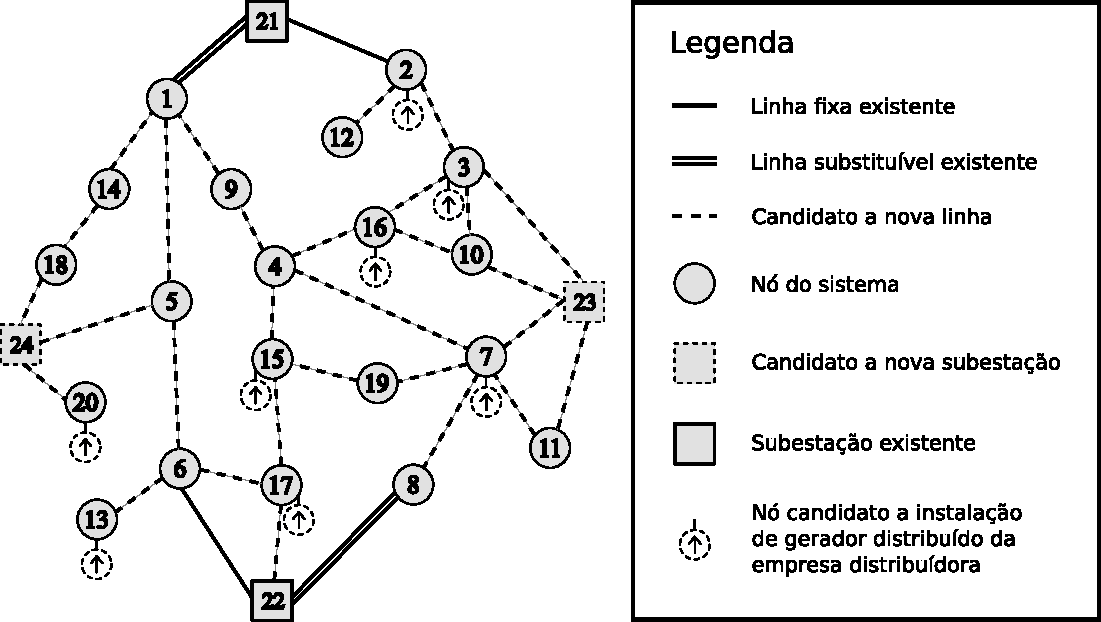
\includegraphics[width=0.8\textwidth]{Anexos/24-bus-system.pdf}\\
    Fonte: Adaptado de \citeonline{MunozDelgado2015}
    \label{fig:24bus}
\end{figure}


Este sistema de distribuição passa por 3 estágios e 3 níveis de carregamento. A tabela \ref{tab:param_carga} apresenta a demanda máxima de cada nó de carga em cada estágio. Note que metade dos barramentos possuem carga já no final do primeiro estágio.
\begin{table}[ht]
\centering
\caption{Demanda máxima do sistema (MVA).}
\label{tab:param_carga}
\begin{tabular}{@{}cccccccc@{}}
\toprule
\multirow{2}{*}{Nó} & \multicolumn{3}{c}{Estágio} & \multirow{2}{*}{Nó} & \multicolumn{3}{c}{Estágio} \\ \cmidrule(lr){2-4} \cmidrule(l){6-8} 
   & 1    & 2    & 3    &    & 1 & 2    & 3    \\ \midrule
1  & 4,05 & 3,45 & 5,42 & 11 & 0 & 1,91 & 2,8  \\
2  & 0,78 & 0,77 & 1,21 & 12 & 0 & 0,93 & 1,29 \\
3  & 2,58 & 3,38 & 3,98 & 13 & 0 & 1,15 & 1,87 \\
4  & 0,32 & 0,41 & 2,43 & 14 & 0 & 3,05 & 3,16 \\
5  & 0,28 & 0,37 & 0,47 & 15 & 0 & 1,62 & 1,62 \\
6  & 1,17 & 0,92 & 1,81 & 16 & 0 & 2,16 & 1,22 \\
7  & 4,04 & 3,7  & 4,36 & 17 & 0 & 0    & 2,4  \\
8  & 0,72 & 0,6  & 0,94 & 18 & 0 & 0    & 2,1  \\
9  & 1,14 & 1,12 & 1,77 & 19 & 0 & 0    & 1,81 \\
10 & 1,56 & 2,04 & 2,4  & 20 & 0 & 0    & 3,79 \\ \bottomrule
\end{tabular}
\\Fonte: Adaptado de \citeonline{MunozDelgado2015}
\end{table}

Já na tabela \ref{tab:param_ramos} são apresentados os comprimentos de cada ramo do sistema, incluindo os ramos existentes.
\begin{table}[ht]
\centering
\caption{Dados dos comprimentos dos ramos (km).}
\label{tab:param_ramos}
\begin{tabular}{@{}ccccccccc@{}}
\toprule
Nó & Nó & Comprimento & Nó & Nó & Comprimento & Nó & Nó & Comprimento \\ \midrule
1  & 5  & 2,22        & 4  & 9  & 1,2         & 7  & 23 & 0,9         \\
1  & 9  & 1,2         & 4  & 15 & 1,6         & 8  & 22 & 1,9         \\
1  & 14 & 1,2         & 4  & 16 & 1,3         & 10 & 16 & 1,6         \\
1  & 21 & 2,2         & 5  & 6  & 2,4         & 10 & 23 & 1,3         \\
2  & 3  & 2           & 5  & 24 & 0,7         & 11 & 23 & 1,6         \\
2  & 12 & 1,1         & 6  & 13 & 1,2         & 14 & 18 & 1           \\
2  & 21 & 1,7         & 6  & 17 & 2,2         & 15 & 17 & 1,2         \\
3  & 10 & 1,1         & 6  & 22 & 2,7         & 15 & 19 & 0,8         \\
3  & 16 & 1,2         & 7  & 8  & 2           & 17 & 22 & 1,5         \\
3  & 23 & 1,2         & 7  & 11 & 1,1         & 18 & 24 & 1,5         \\
4  & 7  & 2,6         & 7  & 19 & 1,2         & 20 & 24 & 0,9         \\ \bottomrule
\end{tabular}
\\Fonte: Adaptado de \citeonline{MunozDelgado2015}
\end{table}

As tabelas \ref{tab:param_trafo}, \ref{tab:param_dg} e \ref{tab:param_linha} apresentam respectivamente os dados dos transformadores, geradores distribuídos e linhas que podem ser instalados neste sistema de distribuição.
\begin{table}[ht]
\centering
\caption{Parâmetros dos candidatos a novos transformadores}
\label{tab:param_trafo}
\begin{tabular}{@{}cccccccc@{}}
\toprule
\multicolumn{4}{c}{Alternativa 1} & \multicolumn{4}{c}{Alternativa 2} \\ \midrule
$\overline{G}^{NT}_1$ & $Z^{NT}_1$ & $C^{M,NT}_1$ & $C^{I,NT}_1$ & $\overline{G}^{NT}_2$ & $Z^{NT}_2$ & $C^{M,NT}_2$ & $C^{I,NT}_2$ \\
(MVA)  & ($\Omega$)  & (USD) & (USD)   & (MVA)  & ($\Omega$)  & (USD) & (USD)   \\ \midrule
12     & 0,16     & 2000 & 750000 & 15     & 0,13     & 3000 & 950000 \\ \bottomrule
\end{tabular}
\\Fonte: Adaptado de \citeonline{MunozDelgado2015}
\end{table}
\begin{table}[ht]
\centering
\caption{Parâmetros dos candidatos a novos geradores distribuídos}
\label{tab:param_dg}
\begin{tabular}{@{}cccccccc@{}}
\toprule
\multicolumn{4}{c}{Alternativa 1}     & \multicolumn{4}{c}{Alternativa 2}     \\ \midrule
$\overline{G}^{DG}_1$ & $C^{I,DG}_1$ & $C^{M,DG}_1$ & $C^{E,DG}_1$ & $\overline{G}^{DG}_2$ & $C^{I,DG}_2$ & $C^{M,DG}_2$ & $C^{E,DG}_2$ \\
(MVA) & ($\frac{\text{USD}}{\text{MWh}}$) & (USD) & ($\frac{\text{USD}}{\text{MWh}}$) & (MVA) & ($\frac{\text{USD}}{\text{MWh}}$)& (USD) & ($\frac{\text{USD}}{\text{MWh}}$) \\ \midrule
1     & 500000    & 22500 & 47        & 2     & 490000    & 44100 & 45        \\ \bottomrule
\end{tabular}
\end{table}
\begin{table}[ht]
\centering
\caption{Parâmetros dos candidatos a linhas}
\label{tab:param_linha}
\begin{tabular}{@{}ccccccc@{}}
\toprule
\multirow{2}{*}{Tipo} & \multicolumn{3}{c}{Alternativa 1}              & \multicolumn{3}{c}{Alternativa 2}              \\ \cmidrule(l){2-7} 
                      & $\overline{F}^{l}_1$ & $Z^{l}_1$ & $C^{I,l}_1$ & $\overline{F}^{l}_2$ & $Z^{l}_2$ & $C^{I,l}_2$ \\ \midrule
$l$ & (MVA) & ($\frac{\Omega}{\text{km}}$) & ($\frac{\text{USD}}{\text{km}}$) & (MVA) & ($\frac{\Omega}{\text{km}}$) & ($\frac{\text{USD}}{\text{km}}$) \\ \midrule
$NRB$                 & 6,28                 & 0,557     & 19140       & 9                    & 0,478     & 29870       \\ \midrule
$NAB$                 & 3,94                 & 0,732     & 15020       & 6,28                 & 0,557     & 25030       \\ \bottomrule
\end{tabular}
\end{table}

\newpage
A tabela \ref{tab:param_carrega} apresenta os dados que se referem ao nível de carregamento do sistema, como o fator de carregamento, duração estimada do nível de carga e custo de compra de energia no nível de carga.
\begin{table}[ht]
\centering
\caption{Parâmetros por nível de carregamento.}
\label{tab:param_carrega}
\begin{tabular}{@{}lccccc@{}}
\toprule
                              &            & \multicolumn{3}{c}{Nível de carregamento} &         \\ \cmidrule(l){2-6} 
Descrição                         & Símbolo    & 1             & 2             & 3             & Unidade \\ \midrule
Fator de carregamento         & $\mu_b$    & 70            & 83            & 100           & \%      \\
Duração estimada              & $\Delta_b$ & 2000          & 5760          & 1000          & h/ano   \\
Custo de energia da subestção & $C^{SS}_b$ & 57,7          & 70            & 85,3          & USD/MWh \\ \bottomrule
\end{tabular}
\\Fonte: Adaptado de \citeonline{MunozDelgado2015}
\end{table}

Por fim, a tabela \ref{tab:param} apresenta outros dados utilizados neste sistema, incluindo os dados financeiros, ativos já instalados, vida útil, etc.
\begin{table}[ht]
\centering
\caption{Parâmetros gerais utilizados}
\label{tab:param}
\begin{tabular}{@{}llccc@{}}
\toprule
 &
  Descrição &
  Símbolo &
  Valor &
  Unidade \\ \midrule
 &
  Taxa de juros &
  $i$ &
  7,1 &
  \% \\
 &
   &
   &
  \multicolumn{1}{l}{} &
  \multicolumn{1}{l}{} \\
 &
  Limite de orçamento &
  $IB_t; \; \forall t \in T$ &
  \multicolumn{1}{l}{6 milhões} &
  USD \\
 &
   &
   &
  \multicolumn{1}{l}{} &
  \multicolumn{1}{l}{} \\
 &
  \begin{tabular}[c]{@{}l@{}}Limite de penetração\\ de geradores\\ distribuídos\end{tabular} &
  $\xi$ &
  25 &
  \% \\
 &
   &
   &
  \multicolumn{1}{l}{} &
  \multicolumn{1}{l}{} \\
 &
  Fator de potência &
  $pf$ &
  0,9 &
  - \\
 &
   &
   &
  \multicolumn{1}{l}{} &
  \multicolumn{1}{l}{} \\
 &
  Tensão base &
  - &
  20 &
  kV \\
 &
   &
   &
  \multicolumn{1}{l}{} &
  \multicolumn{1}{l}{} \\
 &
  \begin{tabular}[c]{@{}l@{}}Limite de tensão \\ superior\end{tabular} &
  $\overline{V}$ &
  1,05 &
  p.u. \\
 &
   &
   &
  \multicolumn{1}{l}{} &
  \multicolumn{1}{l}{} \\
 &
  \begin{tabular}[c]{@{}l@{}}Limite de tensão \\ inferior\end{tabular} &
  $\underline{V}$ &
  0,95 &
  p.u. \\ \midrule
\multirow{7}{*}{\begin{tabular}[c]{@{}l@{}}Dados dos \\ ativos já \\ instalados\end{tabular}} &
  \begin{tabular}[c]{@{}l@{}}Impedância dos \\ transformadores\end{tabular} &
  $Z^{ET}_k; \; \forall k \in K^{ET}$ &
  0,25 &
  $\Omega$ \\
 &
   &
   &
  \multicolumn{1}{l}{} &
  \multicolumn{1}{l}{} \\
 &
  \begin{tabular}[c]{@{}l@{}}Potência nominal \\ dos transformadores\end{tabular} &
  $\overline{G}^{ET}_k; \; \forall k \in K^{ET}$ &
  7,5 &
  MVA \\
 &
   &
   &
  \multicolumn{1}{l}{} &
  \multicolumn{1}{l}{} \\
 &
  \begin{tabular}[c]{@{}l@{}}Ampacidade \\ das linhas\end{tabular} &
  \begin{tabular}[c]{@{}c@{}}$\overline{F}^{l}_k;$\\ $\forall l \in \{EFB,ERB\}, \forall k \in K^{l}$\end{tabular} &
  3,94 &
  MVA \\
 &
   &
   &
  \multicolumn{1}{l}{} &
  \multicolumn{1}{l}{} \\
 &
  \begin{tabular}[c]{@{}l@{}}Impedância \\ das linhas\end{tabular} &
  \begin{tabular}[c]{@{}c@{}}$\overline{Z}^{l}_k; $\\ $\forall l \in \{EFB,ERB\}, \forall k \in K^{l}$\end{tabular} &
  0,732 &
  $\Omega$/km \\ \midrule
\multirow{7}{*}{Vida útil} &
  Subestação &
  $\eta^{SS}$ &
  $\infty^+$ &
  anos \\
 &
   &
   &
  \multicolumn{1}{l}{} &
  \multicolumn{1}{l}{} \\
 &
  Transformador &
  $\eta^{NT}$ &
  15 &
  anos \\
 &
   &
   &
  \multicolumn{1}{l}{} &
  \multicolumn{1}{l}{} \\
 &
  Linhas &
  $\eta^{l}; \;\forall l \in \{NAB, NRB\}$ &
  25 &
  anos \\
 &
   &
   &
  \multicolumn{1}{l}{} &
  \multicolumn{1}{l}{} \\
 &
  Geradores distribuídos &
  $\eta^{DG}$ &
  20 &
  anos \\ \midrule
\multirow{5}{*}{Quantidades} &
  Estágios &
  $n_T$ &
  3 &
  - \\
 &
   &
   &
  \multicolumn{1}{l}{} &
  \multicolumn{1}{l}{} \\
 &
  \begin{tabular}[c]{@{}l@{}}Nós candidatos a \\ receber geradores \\ distribuídos\end{tabular} &
  $n_{DG}$ &
  8 &
  - \\
 &
   &
   &
  \multicolumn{1}{l}{} &
  \multicolumn{1}{l}{} \\
 &
  Partes da linearização &
  $n_\nu$ &
  3 &
  - \\ \bottomrule
\end{tabular}
Fonte: Adaptado de \citeonline{MunozDelgado2015}
\end{table}

% \end{anexosenv}

% ---

\end{document}